\documentclass[twoside]{book}

% Packages required by doxygen
\usepackage{fixltx2e}
\usepackage{calc}
\usepackage{doxygen}
\usepackage[export]{adjustbox} % also loads graphicx
\usepackage{graphicx}
\usepackage[utf8]{inputenc}
\usepackage{makeidx}
\usepackage{multicol}
\usepackage{multirow}
\PassOptionsToPackage{warn}{textcomp}
\usepackage{textcomp}
\usepackage[nointegrals]{wasysym}
\usepackage[table]{xcolor}

% Font selection
\usepackage[T1]{fontenc}
\usepackage[scaled=.90]{helvet}
\usepackage{courier}
\usepackage{amssymb}
\usepackage{sectsty}
\renewcommand{\familydefault}{\sfdefault}
\allsectionsfont{%
  \fontseries{bc}\selectfont%
  \color{darkgray}%
}
\renewcommand{\DoxyLabelFont}{%
  \fontseries{bc}\selectfont%
  \color{darkgray}%
}
\newcommand{\+}{\discretionary{\mbox{\scriptsize$\hookleftarrow$}}{}{}}

% Page & text layout
\usepackage{geometry}
\geometry{%
  a4paper,%
  top=2.5cm,%
  bottom=2.5cm,%
  left=2.5cm,%
  right=2.5cm%
}
\tolerance=750
\hfuzz=15pt
\hbadness=750
\setlength{\emergencystretch}{15pt}
\setlength{\parindent}{0cm}
\setlength{\parskip}{3ex plus 2ex minus 2ex}
\makeatletter
\renewcommand{\paragraph}{%
  \@startsection{paragraph}{4}{0ex}{-1.0ex}{1.0ex}{%
    \normalfont\normalsize\bfseries\SS@parafont%
  }%
}
\renewcommand{\subparagraph}{%
  \@startsection{subparagraph}{5}{0ex}{-1.0ex}{1.0ex}{%
    \normalfont\normalsize\bfseries\SS@subparafont%
  }%
}
\makeatother

% Headers & footers
\usepackage{fancyhdr}
\pagestyle{fancyplain}
\fancyhead[LE]{\fancyplain{}{\bfseries\thepage}}
\fancyhead[CE]{\fancyplain{}{}}
\fancyhead[RE]{\fancyplain{}{\bfseries\leftmark}}
\fancyhead[LO]{\fancyplain{}{\bfseries\rightmark}}
\fancyhead[CO]{\fancyplain{}{}}
\fancyhead[RO]{\fancyplain{}{\bfseries\thepage}}
\fancyfoot[LE]{\fancyplain{}{}}
\fancyfoot[CE]{\fancyplain{}{}}
\fancyfoot[RE]{\fancyplain{}{\bfseries\scriptsize Generated by Doxygen }}
\fancyfoot[LO]{\fancyplain{}{\bfseries\scriptsize Generated by Doxygen }}
\fancyfoot[CO]{\fancyplain{}{}}
\fancyfoot[RO]{\fancyplain{}{}}
\renewcommand{\footrulewidth}{0.4pt}
\renewcommand{\chaptermark}[1]{%
  \markboth{#1}{}%
}
\renewcommand{\sectionmark}[1]{%
  \markright{\thesection\ #1}%
}

% Indices & bibliography
\usepackage{natbib}
\usepackage[titles]{tocloft}
\setcounter{tocdepth}{3}
\setcounter{secnumdepth}{5}
\makeindex

% Hyperlinks (required, but should be loaded last)
\usepackage{ifpdf}
\ifpdf
  \usepackage[pdftex,pagebackref=true]{hyperref}
\else
  \usepackage[ps2pdf,pagebackref=true]{hyperref}
\fi
\hypersetup{%
  colorlinks=true,%
  linkcolor=blue,%
  citecolor=blue,%
  unicode%
}

% Custom commands
\newcommand{\clearemptydoublepage}{%
  \newpage{\pagestyle{empty}\cleardoublepage}%
}

\usepackage{caption}
\captionsetup{labelsep=space,justification=centering,font={bf},singlelinecheck=off,skip=4pt,position=top}

%===== C O N T E N T S =====

\begin{document}

% Titlepage & ToC
\pagenumbering{roman}
\begin{titlepage}
\vspace*{7cm}
\begin{center}%
{\Large superquadric-\/grasp }\\
\vspace*{1cm}
{\large Generated by Doxygen 1.8.11}\\
\end{center}
\end{titlepage}
\clearemptydoublepage
\tableofcontents
\clearemptydoublepage
\pagenumbering{arabic}

%--- Begin generated contents ---
\chapter{Hierarchical Index}
\section{Class Hierarchy}
This inheritance list is sorted roughly, but not completely, alphabetically\+:\begin{DoxyCompactList}
\item \contentsline{section}{Grasp\+Computation}{\pageref{classGraspComputation}}{}
\item \contentsline{section}{Grasp\+Execution}{\pageref{classGraspExecution}}{}
\item \contentsline{section}{grasping\+\_\+\+N\+LP}{\pageref{classgrasping__NLP}}{}
\item \contentsline{section}{Grasp\+Visualization}{\pageref{classGraspVisualization}}{}
\item \contentsline{section}{superquadric\+Grasp\+\_\+\+I\+DL}{\pageref{classsuperquadricGrasp__IDL}}{}
\begin{DoxyCompactList}
\item \contentsline{section}{Grasping\+Module}{\pageref{classGraspingModule}}{}
\end{DoxyCompactList}
\end{DoxyCompactList}

\chapter{Data Structure Index}
\section{Data Structures}
Here are the data structures with brief descriptions\+:\begin{DoxyCompactList}
\item\contentsline{section}{\hyperlink{classGraspComputation}{Grasp\+Computation} \\*This class computes the grasping pose for grasping and object once the superquadric modeling the object is provided }{\pageref{classGraspComputation}}{}
\item\contentsline{section}{\hyperlink{classGraspExecution}{Grasp\+Execution} \\*This class implements the arm movements for reaching the desired pose for grasping the object and for closing the fingers and stably grasping the object by using tactile feedback }{\pageref{classGraspExecution}}{}
\item\contentsline{section}{\hyperlink{classgrasping__NLP}{grasping\+\_\+\+N\+LP} \\*This class computes the grasping pose for a given hand and a superquadric modeling an objct by solving an optimization problem with the Ipopt software package }{\pageref{classgrasping__NLP}}{}
\item\contentsline{section}{\hyperlink{classGraspingModule}{Grasping\+Module} \\*This class handles the grasping pose computation and visualization, together with the interaction with the user }{\pageref{classGraspingModule}}{}
\item\contentsline{section}{\hyperlink{classGraspVisualization}{Grasp\+Visualization} \\*This class shows the computed grasping pose and trajectory overlapped to the camera images }{\pageref{classGraspVisualization}}{}
\item\contentsline{section}{\hyperlink{classsuperquadricGrasp__IDL}{superquadric\+Grasp\+\_\+\+I\+DL} \\*Superquadric\+Grasp\+\_\+\+I\+DL I\+DL Interface to superquadric-\/grasp services }{\pageref{classsuperquadricGrasp__IDL}}{}
\end{DoxyCompactList}

\chapter{Data Structure Documentation}
\section{Grasp\+Computation Class Reference}
\label{classGraspComputation}\index{Grasp\+Computation@{Grasp\+Computation}}


This class computes the grasping pose for grasping and object once the superquadric modeling the object is provided.  




{\ttfamily \#include $<$grasp\+Computation.\+h$>$}

\subsection*{Public Member Functions}
\begin{DoxyCompactItemize}
\item 
{\bfseries Grasp\+Computation} (const yarp\+::os\+::\+Property \&\+\_\+ipopt\+\_\+par, const yarp\+::os\+::\+Property \&\+\_\+pose\+\_\+par, const yarp\+::os\+::\+Property \&\+\_\+trajectory\+\_\+par, const std\+::string \&\+\_\+left\+\_\+or\+\_\+right, yarp\+::sig\+::\+Vector \&\+\_\+hand, yarp\+::sig\+::\+Vector \&\+\_\+hand1, yarp\+::os\+::\+Resource\+Finder $\ast$\+\_\+rf, yarp\+::os\+::\+Property \&\+\_\+complete\+\_\+sol, const yarp\+::sig\+::\+Vector \&\+\_\+object, double \&\+\_\+quality\+\_\+right, double \&\+\_\+quality\+\_\+left)\label{classGraspComputation_a8568147ac89fff96794d84139eb16aa3}

\item 
void \hyperlink{classGraspComputation_a3ae446a26b1620933e071d3a538d742f}{set\+Ipopt\+Par} (const yarp\+::os\+::\+Property \&new\+Options, bool first\+\_\+time)
\begin{DoxyCompactList}\small\item\em Set parameters for computing the solution with ipopt. \end{DoxyCompactList}\item 
yarp\+::os\+::\+Property \hyperlink{classGraspComputation_afbad1962376bdf24b9376cf2c82e0e49}{get\+Ipopt\+Par} ()
\begin{DoxyCompactList}\small\item\em Get parameters used for computing the solution with ipopt. \end{DoxyCompactList}\item 
void \hyperlink{classGraspComputation_a76018ae7258adff6b2efa029fdf6f5dc}{set\+Pose\+Par} (const yarp\+::os\+::\+Property \&new\+Options, bool first\+\_\+time)
\begin{DoxyCompactList}\small\item\em Set parameters for correctly compute the grasping pose. \end{DoxyCompactList}\item 
yarp\+::os\+::\+Property \hyperlink{classGraspComputation_a55cdd807a70b178acc14e1a923ea2feb}{get\+Pose\+Par} ()
\begin{DoxyCompactList}\small\item\em Get parameters for correctly compute the grasping pose. \end{DoxyCompactList}\item 
void \hyperlink{classGraspComputation_a119b778fee99e973e0e9938ba90398a7}{set\+Trajectory\+Par} (const yarp\+::os\+::\+Property \&new\+Options, bool first\+\_\+time)
\begin{DoxyCompactList}\small\item\em Set parameters for correctly compute the trajectory for approaching the desired pose. \end{DoxyCompactList}\item 
yarp\+::os\+::\+Property \hyperlink{classGraspComputation_a9ec71cbbd2fe6165ed4b6d866d78d6be}{get\+Trajectory\+Par} ()
\begin{DoxyCompactList}\small\item\em Get parameters used for correctly compute the trajectory for approaching the desired pose. \end{DoxyCompactList}\item 
bool \hyperlink{classGraspComputation_ad8ea3d70e50ff4f4dbda6b03bcef77fa}{init} ()
\begin{DoxyCompactList}\small\item\em Init function. \end{DoxyCompactList}\item 
void \hyperlink{classGraspComputation_a6a63b1c79c125772f30eb5f82b8437ea}{run} ()\label{classGraspComputation_a6a63b1c79c125772f30eb5f82b8437ea}

\begin{DoxyCompactList}\small\item\em Run function. \end{DoxyCompactList}\item 
bool \hyperlink{classGraspComputation_a28e28e973bd9af1d96bfa7548dc1c029}{compute\+Pose} (yarp\+::sig\+::\+Vector \&\hyperlink{classGraspComputation_a180a48b0a2d730ba28545a18d9f0f7fc}{hand}, const std\+::string \&left\+\_\+or\+\_\+right)
\begin{DoxyCompactList}\small\item\em Compute a given pose for the selected hand. \end{DoxyCompactList}\item 
bool \hyperlink{classGraspComputation_ab68ef4347c7efa9540ab68ff5abf0254}{compute\+Trajectory} (const std\+::string \&chosen\+\_\+hand, const std\+::string \&direction)
\begin{DoxyCompactList}\small\item\em Compute the trajectory for the selected hand. \end{DoxyCompactList}\item 
void \hyperlink{classGraspComputation_a49b0efdf7da5147e987cbf05be135e2f}{get\+Solution} (const std\+::string \&\hyperlink{classGraspComputation_a180a48b0a2d730ba28545a18d9f0f7fc}{hand})
\begin{DoxyCompactList}\small\item\em Extract the solution from ipopt interface. \end{DoxyCompactList}\item 
double \hyperlink{classGraspComputation_a75fcb98c9e15f9aac14ea429f625e662}{get\+Time} ()
\begin{DoxyCompactList}\small\item\em Return computation time for getting the pose. \end{DoxyCompactList}\item 
yarp\+::os\+::\+Property \hyperlink{classGraspComputation_a82ff5a0626b48c45d2fc223ecd16d581}{fill\+Property} (const std\+::string \&\hyperlink{classGraspComputation_a180a48b0a2d730ba28545a18d9f0f7fc}{hand})
\begin{DoxyCompactList}\small\item\em Properly fill a property with the computed solution. \end{DoxyCompactList}\item 
void \hyperlink{classGraspComputation_a5a28918e89faff29fce361c7b5efb58f}{set\+Par} (const std\+::string \&tag, const std\+::string \&value)
\begin{DoxyCompactList}\small\item\em Set a a parameter equal to a value. \end{DoxyCompactList}\item 
void {\bfseries best\+Pose} ()\label{classGraspComputation_ac5d65db1eac887de3513e7e4558cb712}

\end{DoxyCompactItemize}
\subsection*{Data Fields}
\begin{DoxyCompactItemize}
\item 
yarp\+::sig\+::\+Vector \& \hyperlink{classGraspComputation_a180a48b0a2d730ba28545a18d9f0f7fc}{hand}\label{classGraspComputation_a180a48b0a2d730ba28545a18d9f0f7fc}

\begin{DoxyCompactList}\small\item\em Vector for representing one hand ellipsoid. \end{DoxyCompactList}\item 
yarp\+::sig\+::\+Vector \& \hyperlink{classGraspComputation_a8577b68dddb60360dc5ecd1b87440297}{hand1}\label{classGraspComputation_a8577b68dddb60360dc5ecd1b87440297}

\begin{DoxyCompactList}\small\item\em Vector for representing one hand ellipsoid. \end{DoxyCompactList}\item 
yarp\+::os\+::\+Property \& \hyperlink{classGraspComputation_a2a53b7cb2bd19461860d41953bf92c59}{complete\+\_\+sol}\label{classGraspComputation_a2a53b7cb2bd19461860d41953bf92c59}

\begin{DoxyCompactList}\small\item\em Complete solution computed. \end{DoxyCompactList}\item 
const yarp\+::sig\+::\+Vector \& \hyperlink{classGraspComputation_a191eeabb17147b0d091332008fc923c8}{object}\label{classGraspComputation_a191eeabb17147b0d091332008fc923c8}

\begin{DoxyCompactList}\small\item\em Object superquadric. \end{DoxyCompactList}\item 
int {\bfseries count\+\_\+file\+\_\+old}\label{classGraspComputation_a7c13a764201910023cd0ca2800224f4a}

\item 
int {\bfseries count\+\_\+file}\label{classGraspComputation_ad811834d2f0289c1413f0c549205c2f9}

\item 
std\+::string \hyperlink{classGraspComputation_a429ee80f2e9aa3717cf4566cc638b0da}{best\+\_\+hand}\label{classGraspComputation_a429ee80f2e9aa3717cf4566cc638b0da}

\begin{DoxyCompactList}\small\item\em Best hand for grasping the object. \end{DoxyCompactList}\item 
double \hyperlink{classGraspComputation_a7e6cc9e8ace1461121684bcf4c58e3b2}{final\+\_\+value\+\_\+R}\label{classGraspComputation_a7e6cc9e8ace1461121684bcf4c58e3b2}

\begin{DoxyCompactList}\small\item\em Final cost function value for right hand. \end{DoxyCompactList}\item 
double \hyperlink{classGraspComputation_a1a54cde3bbdd7d348f70b3e5ccfaf563}{final\+\_\+value\+\_\+L}\label{classGraspComputation_a1a54cde3bbdd7d348f70b3e5ccfaf563}

\begin{DoxyCompactList}\small\item\em Final cost function value for left hand. \end{DoxyCompactList}\item 
double \hyperlink{classGraspComputation_ac4b645e6f6d6518e933dde2a1c71b126}{cos\+\_\+zr}\label{classGraspComputation_ac4b645e6f6d6518e933dde2a1c71b126}

\begin{DoxyCompactList}\small\item\em Cosing between z axes of the root and right hand reference frame. \end{DoxyCompactList}\item 
double \hyperlink{classGraspComputation_ad6f8257369925e1676f53949717d37d6}{cos\+\_\+zl}\label{classGraspComputation_ad6f8257369925e1676f53949717d37d6}

\begin{DoxyCompactList}\small\item\em Cosing between z axes of the root and right hand reference frame. \end{DoxyCompactList}\item 
double \& \hyperlink{classGraspComputation_a6977630d0dd9437634e22a3b7d71f126}{quality\+\_\+right}\label{classGraspComputation_a6977630d0dd9437634e22a3b7d71f126}

\begin{DoxyCompactList}\small\item\em Quality of pose right. \end{DoxyCompactList}\item 
double \& \hyperlink{classGraspComputation_ab55d63b760c5519cd9434aa143a8efbb}{quality\+\_\+left}\label{classGraspComputation_ab55d63b760c5519cd9434aa143a8efbb}

\begin{DoxyCompactList}\small\item\em Quality of pose left. \end{DoxyCompactList}\end{DoxyCompactItemize}
\subsection*{Protected Attributes}
\begin{DoxyCompactItemize}
\item 
std\+::string \hyperlink{classGraspComputation_a7405e0cd57ad3c0ec2757c0d1e6e791a}{left\+\_\+right}\label{classGraspComputation_a7405e0cd57ad3c0ec2757c0d1e6e791a}

\begin{DoxyCompactList}\small\item\em Hand to be enabled with the code. \end{DoxyCompactList}\item 
std\+::deque$<$ yarp\+::sig\+::\+Vector $>$ \hyperlink{classGraspComputation_ad34b98bdd805de7bbbb92204524fb738}{trajectory\+\_\+right}\label{classGraspComputation_ad34b98bdd805de7bbbb92204524fb738}

\begin{DoxyCompactList}\small\item\em Entire trajectory (final pose and waypoint) for the right hand. \end{DoxyCompactList}\item 
std\+::deque$<$ yarp\+::sig\+::\+Vector $>$ \hyperlink{classGraspComputation_a72729f4e74e28f866121da7ec56645ee}{trajectory\+\_\+left}\label{classGraspComputation_a72729f4e74e28f866121da7ec56645ee}

\begin{DoxyCompactList}\small\item\em Entire trajectory (final pose and waypoint) for the left hand. \end{DoxyCompactList}\item 
yarp\+::sig\+::\+Vector \hyperlink{classGraspComputation_accdb354cf67e5ea2c2189f33bfd2e802}{poseR}\label{classGraspComputation_accdb354cf67e5ea2c2189f33bfd2e802}

\begin{DoxyCompactList}\small\item\em Robot hand pose computed by the solver for the right hand. \end{DoxyCompactList}\item 
yarp\+::sig\+::\+Vector \hyperlink{classGraspComputation_aa8c946727c392c140be73ac1c5e83eb2}{solR}\label{classGraspComputation_aa8c946727c392c140be73ac1c5e83eb2}

\begin{DoxyCompactList}\small\item\em Hand ellipsoid pose computed by the solver for the right hand. \end{DoxyCompactList}\item 
yarp\+::sig\+::\+Vector \hyperlink{classGraspComputation_a7a265ee7cb25e2617108e7128ae0cce5}{poseL}\label{classGraspComputation_a7a265ee7cb25e2617108e7128ae0cce5}

\begin{DoxyCompactList}\small\item\em Robot hand pose computed by the solver for the left hand. \end{DoxyCompactList}\item 
yarp\+::sig\+::\+Vector \hyperlink{classGraspComputation_a0b1a5422bfc7eb04976a8cf4f3a63ed4}{solL}\label{classGraspComputation_a0b1a5422bfc7eb04976a8cf4f3a63ed4}

\begin{DoxyCompactList}\small\item\em Hand ellipsoid pose computed by the solver for the left hand. \end{DoxyCompactList}\item 
double \hyperlink{classGraspComputation_abeab81e105369cb96aa81154dd6deced}{tol}\label{classGraspComputation_abeab81e105369cb96aa81154dd6deced}

\begin{DoxyCompactList}\small\item\em Tolerance of the Ipopt optimization problem. \end{DoxyCompactList}\item 
double \hyperlink{classGraspComputation_a19511014ec2f0e0e91a4d63dc666955b}{constr\+\_\+viol\+\_\+tol}\label{classGraspComputation_a19511014ec2f0e0e91a4d63dc666955b}

\begin{DoxyCompactList}\small\item\em Constraint tolerance of the Ipopt optimization problem. \end{DoxyCompactList}\item 
int \hyperlink{classGraspComputation_ab41a54f337bcd46ecdee9b40a0c964c8}{max\+\_\+iter}\label{classGraspComputation_ab41a54f337bcd46ecdee9b40a0c964c8}

\begin{DoxyCompactList}\small\item\em Maximum iteration allowed for the Ipopt optimization problem. \end{DoxyCompactList}\item 
int \hyperlink{classGraspComputation_a1c8f00915603a90bd1bb405ea9d49ebd}{acceptable\+\_\+iter}\label{classGraspComputation_a1c8f00915603a90bd1bb405ea9d49ebd}

\begin{DoxyCompactList}\small\item\em Acceptable iter of the Ipopt optimization problem. \end{DoxyCompactList}\item 
int {\bfseries object\+\_\+provided}\label{classGraspComputation_adf5c4faf99e9e11cdaf8965fb7da91c4}

\item 
std\+::string \hyperlink{classGraspComputation_ac45140965ecbdce979e455f3e3de7211}{mu\+\_\+strategy}\label{classGraspComputation_ac45140965ecbdce979e455f3e3de7211}

\begin{DoxyCompactList}\small\item\em Mu strategy of the Ipopt optimization problem. \end{DoxyCompactList}\item 
std\+::string \hyperlink{classGraspComputation_a6cf999d26066780519a0f6086b5117aa}{nlp\+\_\+scaling\+\_\+method}\label{classGraspComputation_a6cf999d26066780519a0f6086b5117aa}

\begin{DoxyCompactList}\small\item\em N\+LP scaling method of the Ipopt optimization problem. \end{DoxyCompactList}\item 
double \hyperlink{classGraspComputation_a8a4ee0afa3541485daa338dd25baaa5c}{max\+\_\+cpu\+\_\+time}\label{classGraspComputation_a8a4ee0afa3541485daa338dd25baaa5c}

\begin{DoxyCompactList}\small\item\em Max cpu time allowed for the Ipopt optimization problem. \end{DoxyCompactList}\item 
int \hyperlink{classGraspComputation_afa3a569ce96b4cb1a13020537646ab5a}{n\+\_\+pointshand}\label{classGraspComputation_afa3a569ce96b4cb1a13020537646ab5a}

\begin{DoxyCompactList}\small\item\em Number of points sampled on the hand ellipsoid for the Ipopt optimization problem. \end{DoxyCompactList}\item 
double \hyperlink{classGraspComputation_a0c1bd5e871dfddb9968508fe9bda792c}{distance}\label{classGraspComputation_a0c1bd5e871dfddb9968508fe9bda792c}

\begin{DoxyCompactList}\small\item\em Distance for shifting the waypoint along x axis of the hand reference frame. \end{DoxyCompactList}\item 
double \hyperlink{classGraspComputation_a268253bf8a04a0b05fcb4b02b4af0fbe}{distance1}\label{classGraspComputation_a268253bf8a04a0b05fcb4b02b4af0fbe}

\begin{DoxyCompactList}\small\item\em Distance for shifting the waypoint along z axis of the hand reference frame. \end{DoxyCompactList}\item 
std\+::string \hyperlink{classGraspComputation_a362c9280e813cfcbb1b0b4153fabc88c}{dir}
\begin{DoxyCompactList}\small\item\em Direction for generating the waypoint for the approach\+: it could be on x and z axes (\char`\"{}xz\char`\"{}) or only z axis (\char`\"{}z\char`\"{}) of the hand reference frame. \end{DoxyCompactList}\item 
yarp\+::sig\+::\+Vector \hyperlink{classGraspComputation_a8cc4909b0e1fa249df366926b91bae74}{displacement}\label{classGraspComputation_a8cc4909b0e1fa249df366926b91bae74}

\begin{DoxyCompactList}\small\item\em Distance of the robot pose with respect to the hand ellipsoid along x axis of the hand reference frame. \end{DoxyCompactList}\item 
yarp\+::sig\+::\+Vector \hyperlink{classGraspComputation_ae2f9c475883f512cb132479ee7896a24}{plane}\label{classGraspComputation_ae2f9c475883f512cb132479ee7896a24}

\begin{DoxyCompactList}\small\item\em Parameters of the implicit function describing the plane on which the object is located in the root reference frame. \end{DoxyCompactList}\item 
yarp\+::os\+::\+Property \hyperlink{classGraspComputation_a616f3c17653d2e4d500ce7dbf9849917}{ipopt\+\_\+par}\label{classGraspComputation_a616f3c17653d2e4d500ce7dbf9849917}

\begin{DoxyCompactList}\small\item\em Parameters for the Ipopt optimization problem. \end{DoxyCompactList}\item 
yarp\+::os\+::\+Property \hyperlink{classGraspComputation_a8903e5f9411e6a064d767b4c75c7f3bd}{pose\+\_\+par}\label{classGraspComputation_a8903e5f9411e6a064d767b4c75c7f3bd}

\begin{DoxyCompactList}\small\item\em Parameters for pose computation. \end{DoxyCompactList}\item 
yarp\+::os\+::\+Property \hyperlink{classGraspComputation_a72510e6516dab20c66c39e6eae157f3c}{trajectory\+\_\+par}\label{classGraspComputation_a72510e6516dab20c66c39e6eae157f3c}

\begin{DoxyCompactList}\small\item\em Parameters for trajectory computation. \end{DoxyCompactList}\item 
bool {\bfseries go\+\_\+on}\label{classGraspComputation_a309d4de6f3b04be27ab83e4b32213431}

\item 
double {\bfseries t0}\label{classGraspComputation_a5abf6bd76a8b1a5aee7a49b8ef16a6ac}

\item 
double {\bfseries t\+\_\+grasp}\label{classGraspComputation_a5f5784795d8897981205e4f8e56fe94b}

\item 
yarp\+::os\+::\+Mutex {\bfseries mutex}\label{classGraspComputation_a90ceee41cc255a3e818728228910fec8}

\item 
yarp\+::os\+::\+Resource\+Finder $\ast$ {\bfseries rf}\label{classGraspComputation_a0e0cb4d1a5c490b3da70c2221cb4dd5a}

\item 
int \hyperlink{classGraspComputation_ae79cf636d04cc911176e25edc86b5609}{print\+\_\+level}\label{classGraspComputation_ae79cf636d04cc911176e25edc86b5609}

\begin{DoxyCompactList}\small\item\em Print level for the Ipopt optimization problem. \end{DoxyCompactList}\end{DoxyCompactItemize}


\subsection{Detailed Description}
This class computes the grasping pose for grasping and object once the superquadric modeling the object is provided. 

The solution is given by solving an optimization problem with the Ipopt software package. 

Definition at line 32 of file grasp\+Computation.\+h.



\subsection{Member Function Documentation}
\index{Grasp\+Computation@{Grasp\+Computation}!compute\+Pose@{compute\+Pose}}
\index{compute\+Pose@{compute\+Pose}!Grasp\+Computation@{Grasp\+Computation}}
\subsubsection[{\texorpdfstring{compute\+Pose(yarp\+::sig\+::\+Vector \&hand, const std\+::string \&left\+\_\+or\+\_\+right)}{computePose(yarp::sig::Vector &hand, const std::string &left_or_right)}}]{\setlength{\rightskip}{0pt plus 5cm}bool Grasp\+Computation\+::compute\+Pose (
\begin{DoxyParamCaption}
\item[{yarp\+::sig\+::\+Vector \&}]{hand, }
\item[{const std\+::string \&}]{left\+\_\+or\+\_\+right}
\end{DoxyParamCaption}
)}\label{classGraspComputation_a28e28e973bd9af1d96bfa7548dc1c029}


Compute a given pose for the selected hand. 


\begin{DoxyParams}{Parameters}
{\em hand} & is the hand ellipsoid \\
\hline
{\em left\+\_\+or\+\_\+right} & if the string of the hand\+: right, left or both \\
\hline
\end{DoxyParams}
\begin{DoxyReturn}{Returns}
true/false on success/failure 
\end{DoxyReturn}


Definition at line 444 of file grasp\+Computation.\+cpp.



References grasping\+\_\+\+N\+L\+P\+::init(), and grasping\+\_\+\+N\+L\+P\+::plane.


\begin{DoxyCode}
445 \{
446     stringstream ss;
447     ss << count\_file;
448     \textcolor{keywordtype}{string} count\_file\_string=ss.str();
449 
450     \textcolor{keywordtype}{string} context=this->rf->getHomeContextPath().c\_str();
451     Ipopt::SmartPtr<Ipopt::IpoptApplication> app=\textcolor{keyword}{new} Ipopt::IpoptApplication;
452     app->Options()->SetNumericValue(\textcolor{stringliteral}{"tol"},tol);
453     app->Options()->SetNumericValue(\textcolor{stringliteral}{"constr\_viol\_tol"},constr_viol_tol);
454     app->Options()->SetIntegerValue(\textcolor{stringliteral}{"acceptable\_iter"},acceptable_iter);
455     app->Options()->SetStringValue(\textcolor{stringliteral}{"mu\_strategy"},mu_strategy);
456     app->Options()->SetIntegerValue(\textcolor{stringliteral}{"max\_iter"},max_iter);
457     app->Options()->SetStringValue(\textcolor{stringliteral}{"nlp\_scaling\_method"},nlp_scaling_method);
458     app->Options()->SetStringValue(\textcolor{stringliteral}{"hessian\_approximation"},\textcolor{stringliteral}{"limited-memory"});
459     app->Options()->SetStringValue(\textcolor{stringliteral}{"derivative\_test"},\textcolor{stringliteral}{"first-order"});
460     app->Options()->SetStringValue(\textcolor{stringliteral}{"derivative\_test\_print\_all"},\textcolor{stringliteral}{"yes"});    
461     app->Options()->SetIntegerValue(\textcolor{stringliteral}{"print\_level"},print_level);
462 
463     \textcolor{keywordflow}{if} (print_level > 0)
464         app->Options()->SetStringValue(\textcolor{stringliteral}{"output\_file"}, context+\textcolor{stringliteral}{"/ipopt\_"}+l\_o\_r+\textcolor{stringliteral}{"\_"}+count\_file\_string+\textcolor{stringliteral}{".out"})
      ;
465 
466     app->Initialize();
467 
468     Ipopt::SmartPtr<grasping\_NLP>  grasp\_nlp= \textcolor{keyword}{new} grasping_NLP;
469     grasp\_nlp->init(\textcolor{keywordtype}{object}, which\_hand, n_pointshand, l\_o\_r);
470     grasp\_nlp->configure(this->rf,l\_o\_r, displacement, plane);
471 
472     Ipopt::ApplicationReturnStatus status=app->OptimizeTNLP(GetRawPtr(grasp\_nlp));
473 
474     \textcolor{keywordflow}{if}(status==Ipopt::Solve\_Succeeded)
475     \{
476         \textcolor{keywordflow}{if} (l\_o\_r==\textcolor{stringliteral}{"right"})
477         \{
478             solR=grasp\_nlp->get\_result();
479             final_value_R=grasp\_nlp->get\_final\_F();
480             poseR=grasp\_nlp->robot\_pose;
481             which\_hand=grasp\_nlp->get\_hand();
482 
483             yInfo()<<\textcolor{stringliteral}{"[GraspComputation]: Solution (hand pose) for "}<<l\_o\_r<<\textcolor{stringliteral}{" hand is: "}<<
      poseR.toString(3,3).c\_str();
484             yInfo()<<\textcolor{stringliteral}{"[GraspComputation]: Stretched hand is: "}<<which\_hand.toString(3,3).c\_str();
485 
486             Matrix H=euler2dcm(poseR.subVector(3,5));
487             cos_zr=abs(H(2,2));
488 
489             yInfo()<<\textcolor{stringliteral}{"[GraspComputation]: Inner product between z\_hand and z\_root"}<<abs(H(2,2));
490 
491             yInfo()<<\textcolor{stringliteral}{"[GraspComputation]: Final cost function value"}<<
      final_value_R;
492         \}
493         \textcolor{keywordflow}{else}
494         \{
495             solL=grasp\_nlp->get\_result();
496             final_value_L=grasp\_nlp->get\_final\_F();
497             poseL=grasp\_nlp->robot\_pose;
498             which\_hand=grasp\_nlp->get\_hand();
499             yInfo()<<\textcolor{stringliteral}{"[GraspComputation]: Solution (hand pose) for "}<<l\_o\_r<<\textcolor{stringliteral}{" hand is: "}<<
      poseL.toString(3,3).c\_str();
500 
501             Matrix H=euler2dcm(poseL.subVector(3,5));
502             cos_zl=abs(H(2,2));
503 
504             yInfo()<<\textcolor{stringliteral}{"[GraspComputation]: Inner product between z\_hand and z\_root"}<<abs(H(2,2));
505 
506             yInfo()<<\textcolor{stringliteral}{"[GraspComputation]: Final cost function value"}<<
      final_value_L;
507         \}
508 
509         \textcolor{keywordflow}{return} \textcolor{keyword}{true};
510     \}
511     \textcolor{keywordflow}{else}
512     \{
513         yError()<<\textcolor{stringliteral}{"[GraspComputation]: Problem for "}<<l\_o\_r<<\textcolor{stringliteral}{" not solved!"};
514         \textcolor{keywordflow}{if} (l\_o\_r==\textcolor{stringliteral}{"right"})
515         \{
516             solR.resize(6,0.0);
517             poseR.resize(6,0.0);
518             quality_right=0.0;
519         \}
520 
521         \textcolor{keywordflow}{if} (l\_o\_r==\textcolor{stringliteral}{"left"})
522         \{
523             solL.resize(6,0.0);
524             poseL.resize(6,0.0);
525             quality_left=0.0;
526         \}
527         
528         
529         \textcolor{keywordflow}{return} \textcolor{keyword}{false};
530     \}
531 \}
\end{DoxyCode}
\index{Grasp\+Computation@{Grasp\+Computation}!compute\+Trajectory@{compute\+Trajectory}}
\index{compute\+Trajectory@{compute\+Trajectory}!Grasp\+Computation@{Grasp\+Computation}}
\subsubsection[{\texorpdfstring{compute\+Trajectory(const std\+::string \&chosen\+\_\+hand, const std\+::string \&direction)}{computeTrajectory(const std::string &chosen_hand, const std::string &direction)}}]{\setlength{\rightskip}{0pt plus 5cm}bool Grasp\+Computation\+::compute\+Trajectory (
\begin{DoxyParamCaption}
\item[{const std\+::string \&}]{chosen\+\_\+hand, }
\item[{const std\+::string \&}]{direction}
\end{DoxyParamCaption}
)}\label{classGraspComputation_ab68ef4347c7efa9540ab68ff5abf0254}


Compute the trajectory for the selected hand. 


\begin{DoxyParams}{Parameters}
{\em chosen\+\_\+hand} & is the hand selected for moving  is an option for building the trajectory. It can be \char`\"{}z\char`\"{} or \char`\"{}xz\char`\"{}, according to which direction is used for shifting the trajectory waypoints. \\
\hline
\end{DoxyParams}


Definition at line 534 of file grasp\+Computation.\+cpp.


\begin{DoxyCode}
535 \{
536     Vector pose(6,0.0);
537 
538     \textcolor{keywordflow}{if} (chosen\_hand==\textcolor{stringliteral}{"right"})
539     \{
540         pose=poseR;
541     \}
542     \textcolor{keywordflow}{else}
543         pose=poseL;
544 
545     Vector pose\_rot(6,0.0);
546     Vector euler(3,0.0);
547     euler[0]=pose[3];
548     euler[1]=pose[4];
549     euler[2]=pose[5];
550     Matrix H(4,4);
551     H=euler2dcm(euler);
552     euler[0]=pose[0];
553     euler[1]=pose[1];
554     euler[2]=pose[2];
555     H.setSubcol(euler,0,3);
556 
557     pose\_rot=pose;
558 
559     \textcolor{keywordflow}{if} (direction==\textcolor{stringliteral}{"z"})
560     \{
561         \textcolor{keywordflow}{if} (chosen\_hand==\textcolor{stringliteral}{"right"})
562         \{
563             pose\_rot.setSubvector(0,pose.subVector(0,2)-distance*(H.getCol(2).subVector(0,2)));
564         \}
565         \textcolor{keywordflow}{else}
566         \{
567             pose\_rot.setSubvector(0,pose.subVector(0,2)+distance*(H.getCol(2).subVector(0,2)));
568         \}
569     \}
570     \textcolor{keywordflow}{else} \textcolor{keywordflow}{if} (direction==\textcolor{stringliteral}{"xz"})
571     \{
572         \textcolor{keywordflow}{if} (chosen\_hand==\textcolor{stringliteral}{"right"})
573         \{
574             pose\_rot.setSubvector(0,pose.subVector(0,2)-distance1*(H.getCol(2).subVector(0,2)));
575             pose\_rot.setSubvector(0,pose\_rot.subVector(0,2)-distance*(H.getCol(0).subVector(0,2)));
576         \}
577         \textcolor{keywordflow}{else}
578         \{
579             pose\_rot.setSubvector(0,pose.subVector(0,2)+distance1*(H.getCol(2).subVector(0,2)));
580             pose\_rot.setSubvector(0,pose\_rot.subVector(0,2)-distance*(H.getCol(0).subVector(0,2)));
581         \}
582     \}
583 
584     \textcolor{keywordflow}{if} (chosen\_hand==\textcolor{stringliteral}{"right"})
585     \{
586         trajectory_right.clear();
587 
588         pose.setSubvector(0,pose.subVector(0,2));
589         trajectory_right.push\_back(pose\_rot);
590         trajectory_right.push\_back(pose);
591     \}
592     \textcolor{keywordflow}{else}
593     \{
594         trajectory_left.clear();
595 
596         pose.setSubvector(0,pose.subVector(0,2));
597         trajectory_left.push\_back(pose\_rot);
598         trajectory_left.push\_back(pose);
599     \}
600 
601     \textcolor{keywordflow}{return} \textcolor{keyword}{true};
602 \}
\end{DoxyCode}
\index{Grasp\+Computation@{Grasp\+Computation}!fill\+Property@{fill\+Property}}
\index{fill\+Property@{fill\+Property}!Grasp\+Computation@{Grasp\+Computation}}
\subsubsection[{\texorpdfstring{fill\+Property(const std\+::string \&hand)}{fillProperty(const std::string &hand)}}]{\setlength{\rightskip}{0pt plus 5cm}Property Grasp\+Computation\+::fill\+Property (
\begin{DoxyParamCaption}
\item[{const std\+::string \&}]{hand}
\end{DoxyParamCaption}
)}\label{classGraspComputation_a82ff5a0626b48c45d2fc223ecd16d581}


Properly fill a property with the computed solution. 


\begin{DoxyParams}{Parameters}
{\em hand} & is the hand string \\
\hline
\end{DoxyParams}
\begin{DoxyReturn}{Returns}
the Property with the information inside 
\end{DoxyReturn}


Definition at line 621 of file grasp\+Computation.\+cpp.


\begin{DoxyCode}
622 \{
623     Property poses;
624     Bottle bottle;
625 
626     \textcolor{keywordflow}{if} ((l\_o\_r==\textcolor{stringliteral}{"right"}) || (l\_o\_r==\textcolor{stringliteral}{"both"}))
627     \{
628         Bottle &bottle\_right\_pose=bottle.addList();
629         \textcolor{keywordflow}{for} (\textcolor{keywordtype}{size\_t} i=0; i<poseR.size(); i++)
630         \{
631             bottle\_right\_pose.addDouble(poseR[i]);
632         \}
633         poses.put(\textcolor{stringliteral}{"pose\_right"}, bottle.get(0));
634 
635         Bottle &bottle\_right\_sol=bottle.addList();
636         \textcolor{keywordflow}{for} (\textcolor{keywordtype}{size\_t} i=0; i<solR.size(); i++)
637         \{
638             bottle\_right\_sol.addDouble(solR[i]);
639         \}
640         poses.put(\textcolor{stringliteral}{"solution\_right"}, bottle.get(1));
641 
642         Bottle &bottle\_right\_traj=bottle.addList();
643         \textcolor{keywordflow}{for} (\textcolor{keywordtype}{size\_t} i=0; i<trajectory_right.size(); i++)
644         \{
645             Bottle &bb=bottle\_right\_traj.addList();
646             \textcolor{keywordflow}{for} (\textcolor{keywordtype}{size\_t} j=0; j<trajectory_right[i].size();j++)
647                 bb.addDouble(trajectory_right[i][j]);
648         \}
649         poses.put(\textcolor{stringliteral}{"trajectory\_right"}, bottle.get(2));
650     \}
651 
652     \textcolor{keywordflow}{if} (l\_o\_r==\textcolor{stringliteral}{"both"})
653     \{
654         Bottle &bottle\_left\_pose=bottle.addList();
655         \textcolor{keywordflow}{for} (\textcolor{keywordtype}{size\_t} i=0; i<poseL.size(); i++)
656         \{
657             bottle\_left\_pose.addDouble(poseL[i]);
658         \}
659         poses.put(\textcolor{stringliteral}{"pose\_left"}, bottle.get(3));
660 
661         Bottle &bottle\_left\_sol=bottle.addList();
662         \textcolor{keywordflow}{for} (\textcolor{keywordtype}{size\_t} i=0; i<solL.size(); i++)
663         \{
664             bottle\_left\_sol.addDouble(solL[i]);
665         \}
666         poses.put(\textcolor{stringliteral}{"solution\_left"}, bottle.get(4));
667 
668         Bottle &bottle\_left\_traj=bottle.addList();
669         \textcolor{keywordflow}{for} (\textcolor{keywordtype}{size\_t} i=0; i<trajectory_left.size(); i++)
670         \{
671             Bottle &bb=bottle\_left\_traj.addList();
672             \textcolor{keywordflow}{for} (\textcolor{keywordtype}{size\_t} j=0; j<trajectory_left[i].size();j++)
673                 bb.addDouble(trajectory_left[i][j]);
674         \}
675         poses.put(\textcolor{stringliteral}{"trajectory\_left"}, bottle.get(5));
676     \}
677     \textcolor{keywordflow}{if} (l\_o\_r==\textcolor{stringliteral}{"left"})
678     \{
679         Bottle &bottle\_left\_pose=bottle.addList();
680         \textcolor{keywordflow}{for} (\textcolor{keywordtype}{size\_t} i=0; i<poseL.size(); i++)
681         \{
682             bottle\_left\_pose.addDouble(poseL[i]);
683         \}
684         poses.put(\textcolor{stringliteral}{"pose\_left"}, bottle.get(0));
685 
686         Bottle &bottle\_left\_sol=bottle.addList();
687         \textcolor{keywordflow}{for} (\textcolor{keywordtype}{size\_t} i=0; i<solL.size(); i++)
688         \{
689             bottle\_left\_sol.addDouble(solL[i]);
690         \}
691         poses.put(\textcolor{stringliteral}{"solution\_left"}, bottle.get(1));
692 
693         Bottle &bottle\_left\_traj=bottle.addList();
694         \textcolor{keywordflow}{for} (\textcolor{keywordtype}{size\_t} i=0; i<trajectory_left.size(); i++)
695         \{
696             Bottle &bb=bottle\_left\_traj.addList();
697             \textcolor{keywordflow}{for} (\textcolor{keywordtype}{size\_t} j=0; j<trajectory_left[i].size();j++)
698                 bb.addDouble(trajectory_left[i][j]);
699         \}
700         poses.put(\textcolor{stringliteral}{"trajectory\_left"}, bottle.get(2));
701     \}
702 
703     \textcolor{keywordflow}{return} poses;
704 \}
\end{DoxyCode}
\index{Grasp\+Computation@{Grasp\+Computation}!get\+Ipopt\+Par@{get\+Ipopt\+Par}}
\index{get\+Ipopt\+Par@{get\+Ipopt\+Par}!Grasp\+Computation@{Grasp\+Computation}}
\subsubsection[{\texorpdfstring{get\+Ipopt\+Par()}{getIpoptPar()}}]{\setlength{\rightskip}{0pt plus 5cm}Property Grasp\+Computation\+::get\+Ipopt\+Par (
\begin{DoxyParamCaption}
{}
\end{DoxyParamCaption}
)}\label{classGraspComputation_afbad1962376bdf24b9376cf2c82e0e49}


Get parameters used for computing the solution with ipopt. 

\begin{DoxyReturn}{Returns}
a Property with all the options for ipopt 
\end{DoxyReturn}


Definition at line 194 of file grasp\+Computation.\+cpp.


\begin{DoxyCode}
195 \{
196     LockGuard lg(mutex);
197 
198     Property advOptions;
199     advOptions.put(\textcolor{stringliteral}{"max\_cpu\_time"},max_cpu_time);
200     advOptions.put(\textcolor{stringliteral}{"tol"},tol);
201     advOptions.put(\textcolor{stringliteral}{"max\_iter"},max_iter);
202     advOptions.put(\textcolor{stringliteral}{"acceptable\_iter"},acceptable_iter);
203     advOptions.put(\textcolor{stringliteral}{"IPOPT\_mu\_strategy"},mu_strategy);
204     advOptions.put(\textcolor{stringliteral}{"IPOPT\_nlp\_scaling\_method"},nlp_scaling_method);
205     advOptions.put(\textcolor{stringliteral}{"IPOPT\_print\_level"}, print_level);
206     \textcolor{keywordflow}{return} advOptions;
207 \}
\end{DoxyCode}
\index{Grasp\+Computation@{Grasp\+Computation}!get\+Pose\+Par@{get\+Pose\+Par}}
\index{get\+Pose\+Par@{get\+Pose\+Par}!Grasp\+Computation@{Grasp\+Computation}}
\subsubsection[{\texorpdfstring{get\+Pose\+Par()}{getPosePar()}}]{\setlength{\rightskip}{0pt plus 5cm}Property Grasp\+Computation\+::get\+Pose\+Par (
\begin{DoxyParamCaption}
{}
\end{DoxyParamCaption}
)}\label{classGraspComputation_a55cdd807a70b178acc14e1a923ea2feb}


Get parameters for correctly compute the grasping pose. 

\begin{DoxyReturn}{Returns}
a Property with all the options for pose computation 
\end{DoxyReturn}


Definition at line 284 of file grasp\+Computation.\+cpp.



References grasping\+\_\+\+N\+L\+P\+::plane.


\begin{DoxyCode}
285 \{
286     LockGuard lg(mutex);
287 
288     Property advOptions;
289     advOptions.put(\textcolor{stringliteral}{"n\_pointshand"},n_pointshand);
290 
291     Bottle bottle\_disp;
292     Bottle &bottle\_displacement=bottle\_disp.addList();
293     bottle\_displacement.addDouble(displacement[0]); bottle\_displacement.addDouble(
      displacement[1]);
294     bottle\_displacement.addDouble(displacement[2]);
295     advOptions.put(\textcolor{stringliteral}{"hand\_displacement"},bottle\_disp.get(0));
296 
297     Bottle bottle\_pl;
298     Bottle &bottle\_plane=bottle\_pl.addList();
299     bottle\_plane.addDouble(plane[0]); bottle\_plane.addDouble(plane[1]);
300     bottle\_plane.addDouble(plane[2]); bottle\_plane.addDouble(plane[3]);
301     advOptions.put(\textcolor{stringliteral}{"plane"}, bottle\_pl.get(0));
302 
303     \textcolor{keywordflow}{return} advOptions;
304 \}
\end{DoxyCode}
\index{Grasp\+Computation@{Grasp\+Computation}!get\+Solution@{get\+Solution}}
\index{get\+Solution@{get\+Solution}!Grasp\+Computation@{Grasp\+Computation}}
\subsubsection[{\texorpdfstring{get\+Solution(const std\+::string \&hand)}{getSolution(const std::string &hand)}}]{\setlength{\rightskip}{0pt plus 5cm}void Grasp\+Computation\+::get\+Solution (
\begin{DoxyParamCaption}
\item[{const std\+::string \&}]{hand}
\end{DoxyParamCaption}
)}\label{classGraspComputation_a49b0efdf7da5147e987cbf05be135e2f}


Extract the solution from ipopt interface. 


\begin{DoxyParams}{Parameters}
{\em hand} & is the selected hand \\
\hline
\end{DoxyParams}


Definition at line 613 of file grasp\+Computation.\+cpp.


\begin{DoxyCode}
614 \{
615     LockGuard lg(mutex);
616 
617     complete_sol=fillProperty(hand);
618 \}
\end{DoxyCode}
\index{Grasp\+Computation@{Grasp\+Computation}!get\+Time@{get\+Time}}
\index{get\+Time@{get\+Time}!Grasp\+Computation@{Grasp\+Computation}}
\subsubsection[{\texorpdfstring{get\+Time()}{getTime()}}]{\setlength{\rightskip}{0pt plus 5cm}double Grasp\+Computation\+::get\+Time (
\begin{DoxyParamCaption}
{}
\end{DoxyParamCaption}
)}\label{classGraspComputation_a75fcb98c9e15f9aac14ea429f625e662}


Return computation time for getting the pose. 

\begin{DoxyReturn}{Returns}
the period value 
\end{DoxyReturn}


Definition at line 605 of file grasp\+Computation.\+cpp.


\begin{DoxyCode}
606 \{
607     LockGuard lg(mutex);
608     
609     \textcolor{keywordflow}{return} t\_grasp;
610 \}
\end{DoxyCode}
\index{Grasp\+Computation@{Grasp\+Computation}!get\+Trajectory\+Par@{get\+Trajectory\+Par}}
\index{get\+Trajectory\+Par@{get\+Trajectory\+Par}!Grasp\+Computation@{Grasp\+Computation}}
\subsubsection[{\texorpdfstring{get\+Trajectory\+Par()}{getTrajectoryPar()}}]{\setlength{\rightskip}{0pt plus 5cm}Property Grasp\+Computation\+::get\+Trajectory\+Par (
\begin{DoxyParamCaption}
{}
\end{DoxyParamCaption}
)}\label{classGraspComputation_a9ec71cbbd2fe6165ed4b6d866d78d6be}


Get parameters used for correctly compute the trajectory for approaching the desired pose. 

\begin{DoxyReturn}{Returns}
a Property with all the options for pose computation 
\end{DoxyReturn}


Definition at line 372 of file grasp\+Computation.\+cpp.


\begin{DoxyCode}
373 \{
374     LockGuard lg(mutex);
375 
376     Property advOptions;
377     advOptions.put(\textcolor{stringliteral}{"distance\_on\_x"},distance);
378     advOptions.put(\textcolor{stringliteral}{"distance\_on\_z"},distance1);
379     advOptions.put(\textcolor{stringliteral}{"approaching\_direction"},dir);
380 
381     \textcolor{keywordflow}{return} advOptions;
382 \}
\end{DoxyCode}
\index{Grasp\+Computation@{Grasp\+Computation}!init@{init}}
\index{init@{init}!Grasp\+Computation@{Grasp\+Computation}}
\subsubsection[{\texorpdfstring{init()}{init()}}]{\setlength{\rightskip}{0pt plus 5cm}bool Grasp\+Computation\+::init (
\begin{DoxyParamCaption}
{}
\end{DoxyParamCaption}
)}\label{classGraspComputation_ad8ea3d70e50ff4f4dbda6b03bcef77fa}


Init function. 

\begin{DoxyReturn}{Returns}
true/false on success/failure 
\end{DoxyReturn}


Definition at line 385 of file grasp\+Computation.\+cpp.


\begin{DoxyCode}
386 \{
387     yInfo()<<\textcolor{stringliteral}{"[GraspComputation]: Thread initing ... "};
388 
389     setIpoptPar(ipopt_par,\textcolor{keyword}{true});
390     setPosePar(pose_par, \textcolor{keyword}{true});
391     setTrajectoryPar(trajectory_par, \textcolor{keyword}{true});
392 
393     solR.resize(11,0.0);
394     solL.resize(11,0.0);
395     poseR.resize(6,0.0);
396     poseL.resize(6,0.0);
397 
398     go\_on=\textcolor{keyword}{false};
399 
400     count\_file=0;
401 
402     \textcolor{keywordflow}{return} \textcolor{keyword}{true};
403 \}
\end{DoxyCode}
\index{Grasp\+Computation@{Grasp\+Computation}!set\+Ipopt\+Par@{set\+Ipopt\+Par}}
\index{set\+Ipopt\+Par@{set\+Ipopt\+Par}!Grasp\+Computation@{Grasp\+Computation}}
\subsubsection[{\texorpdfstring{set\+Ipopt\+Par(const yarp\+::os\+::\+Property \&new\+Options, bool first\+\_\+time)}{setIpoptPar(const yarp::os::Property &newOptions, bool first_time)}}]{\setlength{\rightskip}{0pt plus 5cm}void Grasp\+Computation\+::set\+Ipopt\+Par (
\begin{DoxyParamCaption}
\item[{const yarp\+::os\+::\+Property \&}]{new\+Options, }
\item[{bool}]{first\+\_\+time}
\end{DoxyParamCaption}
)}\label{classGraspComputation_a3ae446a26b1620933e071d3a538d742f}


Set parameters for computing the solution with ipopt. 


\begin{DoxyParams}{Parameters}
{\em new\+Options} & is a Property with the new options to be set \\
\hline
{\em first\+\_\+time} & takes into account if it is the first the options are set or not \\
\hline
\end{DoxyParams}


Definition at line 32 of file grasp\+Computation.\+cpp.


\begin{DoxyCode}
33 \{
34     LockGuard lg(mutex);
35 
36     \textcolor{keywordtype}{double} maxCpuTime=newOptions.find(\textcolor{stringliteral}{"max\_cpu\_time"}).asDouble();
37     \textcolor{keywordflow}{if} (newOptions.find(\textcolor{stringliteral}{"max\_cpu\_time"}).isNull() && (first\_time==\textcolor{keyword}{true}))
38     \{
39         max_cpu_time=5.0;
40     \}
41     \textcolor{keywordflow}{else} \textcolor{keywordflow}{if} (!newOptions.find(\textcolor{stringliteral}{"max\_cpu\_time"}).isNull())
42     \{
43         \textcolor{keywordflow}{if} ((maxCpuTime>=0.01) && (maxCpuTime<=10.0))
44         \{
45             max_cpu_time=maxCpuTime;
46         \}
47         \textcolor{keywordflow}{else} \textcolor{keywordflow}{if} (maxCpuTime<0.01)
48         \{
49             max_cpu_time=0.01;
50         \}
51         \textcolor{keywordflow}{else} \textcolor{keywordflow}{if} (maxCpuTime>10.0)
52         \{
53             max_cpu_time=10.0;
54         \}
55     \}
56 
57     \textcolor{keywordtype}{double} tolValue=newOptions.find(\textcolor{stringliteral}{"tol"}).asDouble();
58     \textcolor{keywordflow}{if} (newOptions.find(\textcolor{stringliteral}{"tol"}).isNull() && (first\_time==\textcolor{keyword}{true}))
59     \{
60         tol=1e-5;
61     \}
62     \textcolor{keywordflow}{else} \textcolor{keywordflow}{if} (!newOptions.find(\textcolor{stringliteral}{"tol"}).isNull())
63     \{
64         \textcolor{keywordflow}{if} ((tolValue>1e-8) && (tolValue<=0.01))
65         \{
66             tol=tolValue;
67         \}
68         \textcolor{keywordflow}{else} \textcolor{keywordflow}{if} (tolValue<1e-8)
69         \{
70             tol=1e-8;
71         \}
72         \textcolor{keywordflow}{else} \textcolor{keywordflow}{if} (tolValue>0.01)
73         \{
74             tol=0.01;
75         \}
76     \}
77 
78     \textcolor{keywordtype}{double} constrTolValue=newOptions.find(\textcolor{stringliteral}{"constr\_viol\_tol"}).asDouble();
79     \textcolor{keywordflow}{if} (newOptions.find(\textcolor{stringliteral}{"constr\_viol\_tol"}).isNull() && (first\_time==\textcolor{keyword}{true}))
80     \{
81         constr_viol_tol=1e-5;
82     \}
83     \textcolor{keywordflow}{else} \textcolor{keywordflow}{if} (!newOptions.find(\textcolor{stringliteral}{"constr\_viol\_tol"}).isNull())
84     \{
85         \textcolor{keywordflow}{if} ((constrTolValue>1e-8) && (constrTolValue<=0.01))
86         \{
87             constr_viol_tol=constrTolValue;
88         \}
89         \textcolor{keywordflow}{else} \textcolor{keywordflow}{if} (constrTolValue<1e-8)
90         \{
91             constr_viol_tol=1e-8;
92         \}
93         \textcolor{keywordflow}{else} \textcolor{keywordflow}{if} (constrTolValue>0.01)
94         \{
95             constr_viol_tol=0.01;
96         \}
97     \}
98 
99     \textcolor{keywordtype}{int} accIter=newOptions.find(\textcolor{stringliteral}{"acceptable\_iter"}).asInt();
100     \textcolor{keywordflow}{if} (newOptions.find(\textcolor{stringliteral}{"acceptable\_iter"}).isNull() && (first\_time==\textcolor{keyword}{true}))
101     \{
102         acceptable_iter=0;
103     \}
104     \textcolor{keywordflow}{else} \textcolor{keywordflow}{if} (!newOptions.find(\textcolor{stringliteral}{"acceptable\_iter"}).isNull())
105     \{
106         \textcolor{keywordflow}{if} ((accIter>=0 )&& (accIter<=10))
107         \{
108              acceptable_iter=accIter;
109         \}
110         \textcolor{keywordflow}{else} \textcolor{keywordflow}{if} (accIter<0 )
111         \{
112             acceptable_iter=0;
113         \}
114         \textcolor{keywordflow}{else} \textcolor{keywordflow}{if} (accIter>10)
115         \{
116             acceptable_iter=10;
117         \}
118     \}
119 
120     \textcolor{keywordtype}{int} maxIter=newOptions.find(\textcolor{stringliteral}{"max\_iter"}).asInt();
121     \textcolor{keywordflow}{if} (newOptions.find(\textcolor{stringliteral}{"max\_iter"}).isNull() && (first\_time==\textcolor{keyword}{true}))
122     \{
123         max_iter=100;
124     \}
125     \textcolor{keywordflow}{else} \textcolor{keywordflow}{if} (!newOptions.find(\textcolor{stringliteral}{"max\_iter"}).isNull())
126     \{
127         \textcolor{keywordflow}{if} ((maxIter>1))
128         \{
129             max_iter=maxIter;
130         \}
131         \textcolor{keywordflow}{else}
132         \{
133             max_iter=100;
134         \}
135     \}
136 
137     \textcolor{keywordtype}{string} mu\_str=newOptions.find(\textcolor{stringliteral}{"mu\_strategy"}).asString();
138     \textcolor{keywordflow}{if} (newOptions.find(\textcolor{stringliteral}{"mu\_strategy"}).isNull() && (first\_time==\textcolor{keyword}{true}))
139     \{
140         mu_strategy=\textcolor{stringliteral}{"monotone"};
141     \}
142     \textcolor{keywordflow}{else} \textcolor{keywordflow}{if} (!newOptions.find(\textcolor{stringliteral}{"mu\_strategy"}).isNull())
143     \{
144         \textcolor{keywordflow}{if} ((mu\_str==\textcolor{stringliteral}{"adaptive"}) || (mu\_str==\textcolor{stringliteral}{"monotone"}))
145         \{
146             mu_strategy=mu\_str;
147         \}
148         \textcolor{keywordflow}{else}
149         \{
150             mu_strategy=\textcolor{stringliteral}{"monotone"};
151         \}
152     \}
153 
154     \textcolor{keywordtype}{string} nlp=newOptions.find(\textcolor{stringliteral}{"nlp\_scaling\_method"}).asString();
155     \textcolor{keywordflow}{if} (newOptions.find(\textcolor{stringliteral}{"nlp\_scaling\_method"}).isNull() && (first\_time==\textcolor{keyword}{true}))
156     \{
157         nlp_scaling_method=\textcolor{stringliteral}{"gradient-based"};
158     \}
159     \textcolor{keywordflow}{else} \textcolor{keywordflow}{if} (!newOptions.find(\textcolor{stringliteral}{"nlp\_scaling\_method"}).isNull())
160     \{
161         \textcolor{keywordflow}{if} ((nlp==\textcolor{stringliteral}{"none"}) || (nlp==\textcolor{stringliteral}{"gradient-based"}))
162         \{
163             nlp_scaling_method=nlp;
164         \}
165         \textcolor{keywordflow}{else}
166         \{
167             nlp_scaling_method=\textcolor{stringliteral}{"gradient-based"};
168         \}
169     \}
170 
171     \textcolor{keywordtype}{int} pl=newOptions.find(\textcolor{stringliteral}{"print\_level"}).asInt();
172     \textcolor{keywordflow}{if} (newOptions.find(\textcolor{stringliteral}{"print\_level"}).isNull() && (first\_time==\textcolor{keyword}{true}))
173     \{
174         print_level=0;
175     \}
176     \textcolor{keywordflow}{else} \textcolor{keywordflow}{if} (!newOptions.find(\textcolor{stringliteral}{"print\_level"}).isNull())
177     \{
178         \textcolor{keywordflow}{if} ((pl>=0 )&& (pl<=10))
179         \{
180              print_level=pl;
181         \}
182         \textcolor{keywordflow}{else} \textcolor{keywordflow}{if} (pl<0 )
183         \{
184             pl=0;
185         \}
186         \textcolor{keywordflow}{else} \textcolor{keywordflow}{if} (pl>10)
187         \{
188             print_level=10;
189         \}
190     \}
191 \}
\end{DoxyCode}
\index{Grasp\+Computation@{Grasp\+Computation}!set\+Par@{set\+Par}}
\index{set\+Par@{set\+Par}!Grasp\+Computation@{Grasp\+Computation}}
\subsubsection[{\texorpdfstring{set\+Par(const std\+::string \&tag, const std\+::string \&value)}{setPar(const std::string &tag, const std::string &value)}}]{\setlength{\rightskip}{0pt plus 5cm}void Grasp\+Computation\+::set\+Par (
\begin{DoxyParamCaption}
\item[{const std\+::string \&}]{tag, }
\item[{const std\+::string \&}]{value}
\end{DoxyParamCaption}
)}\label{classGraspComputation_a5a28918e89faff29fce361c7b5efb58f}


Set a a parameter equal to a value. 


\begin{DoxyParams}{Parameters}
{\em tag} & is the name of the parameter \\
\hline
{\em value} & is the new value of parameter \\
\hline
\end{DoxyParams}


Definition at line 707 of file grasp\+Computation.\+cpp.


\begin{DoxyCode}
708 \{
709     \textcolor{keywordflow}{if} (par\_name==\textcolor{stringliteral}{"left\_or\_right"})
710         left_right=value;
711 \}
\end{DoxyCode}
\index{Grasp\+Computation@{Grasp\+Computation}!set\+Pose\+Par@{set\+Pose\+Par}}
\index{set\+Pose\+Par@{set\+Pose\+Par}!Grasp\+Computation@{Grasp\+Computation}}
\subsubsection[{\texorpdfstring{set\+Pose\+Par(const yarp\+::os\+::\+Property \&new\+Options, bool first\+\_\+time)}{setPosePar(const yarp::os::Property &newOptions, bool first_time)}}]{\setlength{\rightskip}{0pt plus 5cm}void Grasp\+Computation\+::set\+Pose\+Par (
\begin{DoxyParamCaption}
\item[{const yarp\+::os\+::\+Property \&}]{new\+Options, }
\item[{bool}]{first\+\_\+time}
\end{DoxyParamCaption}
)}\label{classGraspComputation_a76018ae7258adff6b2efa029fdf6f5dc}


Set parameters for correctly compute the grasping pose. 


\begin{DoxyParams}{Parameters}
{\em new\+Options} & is a Property with the new options to be set \\
\hline
{\em first\+\_\+time} & takes into account if it is the first the options are set or not \\
\hline
\end{DoxyParams}


Definition at line 210 of file grasp\+Computation.\+cpp.



References grasping\+\_\+\+N\+L\+P\+::plane.



Referenced by Grasp\+Execution\+::configure().


\begin{DoxyCode}
211 \{
212     LockGuard lg(mutex);
213     \textcolor{keywordflow}{if} (first\_time)
214     \{
215         displacement.resize(3,0.0);
216         plane.resize(4,0.0);
217     \}
218 
219     \textcolor{keywordtype}{int} points=newOptions.find(\textcolor{stringliteral}{"n\_pointshand"}).asInt();
220 
221     \textcolor{keywordflow}{if} (newOptions.find(\textcolor{stringliteral}{"n\_pointshand"}).isNull() && (first\_time==\textcolor{keyword}{true}))
222     \{
223         n_pointshand=46;
224     \}
225     \textcolor{keywordflow}{else} \textcolor{keywordflow}{if} (!newOptions.find(\textcolor{stringliteral}{"n\_pointshand"}).isNull())
226     \{
227         \textcolor{keywordflow}{if} ((points>=4) && (points<=100))
228         \{
229             n_pointshand=points;
230         \}
231         \textcolor{keywordflow}{else} \textcolor{keywordflow}{if} (points<4)
232         \{
233             n_pointshand=4;
234         \}
235         \textcolor{keywordflow}{else} \textcolor{keywordflow}{if} (points>100)
236         \{
237             n_pointshand=100;
238         \}
239     \}
240 
241     Bottle *disp=newOptions.find(\textcolor{stringliteral}{"hand\_displacement"}).asList();
242     \textcolor{keywordflow}{if} (newOptions.find(\textcolor{stringliteral}{"hand\_displacement"}).isNull() && (first\_time==\textcolor{keyword}{true}))
243     \{
244         displacement[0]=0.05;
245         displacement[1]=0.0;
246         displacement[2]=0.0;
247     \}
248     \textcolor{keywordflow}{else} \textcolor{keywordflow}{if} (!newOptions.find(\textcolor{stringliteral}{"hand\_displacement"}).isNull())
249     \{
250         Vector tmp(3,0.0);
251         tmp[0]=disp->get(0).asDouble();
252         tmp[1]=disp->get(1).asDouble();
253         tmp[2]=disp->get(2).asDouble();
254 
255         displacement=tmp;
256 
257     \}
258 
259     Bottle *pl=newOptions.find(\textcolor{stringliteral}{"plane"}).asList();
260 
261     \textcolor{keywordflow}{if} (newOptions.find(\textcolor{stringliteral}{"plane"}).isNull() && (first\_time==\textcolor{keyword}{true}))
262     \{
263         plane[0]=0.0; plane[1]=0.0; plane[2]=1.0; plane[3]=0.11;
264     \}
265     \textcolor{keywordflow}{else} \textcolor{keywordflow}{if} (!newOptions.find(\textcolor{stringliteral}{"plane"}).isNull())
266     \{
267         Vector tmp(4,0.0);
268         tmp[0]=pl->get(0).asDouble();
269         tmp[1]=pl->get(1).asDouble();
270         tmp[2]=pl->get(2).asDouble();
271         tmp[3]=pl->get(3).asDouble();
272         \textcolor{keywordflow}{if} (norm(tmp)>0.0)
273         \{
274             plane=tmp;
275         \}
276         \textcolor{keywordflow}{else}
277         \{
278             plane[0]=0.0; plane[1]=0.0; plane[2]=1.0; plane[3]=0.11;
279         \}
280     \}
281 \}
\end{DoxyCode}
\index{Grasp\+Computation@{Grasp\+Computation}!set\+Trajectory\+Par@{set\+Trajectory\+Par}}
\index{set\+Trajectory\+Par@{set\+Trajectory\+Par}!Grasp\+Computation@{Grasp\+Computation}}
\subsubsection[{\texorpdfstring{set\+Trajectory\+Par(const yarp\+::os\+::\+Property \&new\+Options, bool first\+\_\+time)}{setTrajectoryPar(const yarp::os::Property &newOptions, bool first_time)}}]{\setlength{\rightskip}{0pt plus 5cm}void Grasp\+Computation\+::set\+Trajectory\+Par (
\begin{DoxyParamCaption}
\item[{const yarp\+::os\+::\+Property \&}]{new\+Options, }
\item[{bool}]{first\+\_\+time}
\end{DoxyParamCaption}
)}\label{classGraspComputation_a119b778fee99e973e0e9938ba90398a7}


Set parameters for correctly compute the trajectory for approaching the desired pose. 


\begin{DoxyParams}{Parameters}
{\em new\+Options} & is a Property with the new options to be set \\
\hline
{\em first\+\_\+time} & takes into account if it is the first the options are set or not \\
\hline
\end{DoxyParams}


Definition at line 307 of file grasp\+Computation.\+cpp.


\begin{DoxyCode}
308 \{
309     LockGuard lg(mutex);
310 
311     \textcolor{keywordtype}{double} dist=newOptions.find(\textcolor{stringliteral}{"distance\_on\_x"}).asDouble();
312     \textcolor{keywordflow}{if} (newOptions.find(\textcolor{stringliteral}{"distance\_on\_x"}).isNull() && (first\_time==\textcolor{keyword}{true}))
313     \{
314         distance=0.13;
315     \}
316     \textcolor{keywordflow}{else} \textcolor{keywordflow}{if} (!newOptions.find(\textcolor{stringliteral}{"distance\_on\_x"}).isNull())
317     \{
318         \textcolor{keywordflow}{if} ((dist>=0.0) && (dist<=0.3))
319         \{
320             distance=dist;
321         \}
322         \textcolor{keywordflow}{else} \textcolor{keywordflow}{if} (dist<0.0)
323         \{
324             distance=0.0;
325         \}
326         \textcolor{keywordflow}{else} \textcolor{keywordflow}{if} (dist>0.3)
327         \{
328             distance=0.3;
329         \}
330     \}
331 
332     dist=newOptions.find(\textcolor{stringliteral}{"distance\_on\_z"}).asDouble();
333     \textcolor{keywordflow}{if} (newOptions.find(\textcolor{stringliteral}{"distance\_on\_z"}).isNull() && (first\_time==\textcolor{keyword}{true}))
334     \{
335         distance1=0.05;
336     \}
337     \textcolor{keywordflow}{else} \textcolor{keywordflow}{if} (!newOptions.find(\textcolor{stringliteral}{"distance\_on\_z"}).isNull())
338     \{
339         \textcolor{keywordflow}{if} ((dist>=0.0) && (dist<=0.3))
340         \{
341             distance1=dist;
342         \}
343         \textcolor{keywordflow}{else} \textcolor{keywordflow}{if} (dist<0.0)
344         \{
345             distance1=0.0;
346         \}
347         \textcolor{keywordflow}{else} \textcolor{keywordflow}{if} (dist>0.3)
348         \{
349             distance1=0.3;
350         \}
351     \}
352 
353     \textcolor{keywordtype}{string} direct=newOptions.find(\textcolor{stringliteral}{"approaching\_direction"}).asString();
354     \textcolor{keywordflow}{if} (newOptions.find(\textcolor{stringliteral}{"approaching\_direction"}).isNull() && (first\_time==\textcolor{keyword}{true}))
355     \{
356         dir=direct;
357     \}
358     \textcolor{keywordflow}{else} \textcolor{keywordflow}{if} (!newOptions.find(\textcolor{stringliteral}{"approaching\_direction"}).isNull())
359     \{
360         \textcolor{keywordflow}{if} (direct==\textcolor{stringliteral}{"z"})
361         \{
362             dir=direct;
363         \}
364         \textcolor{keywordflow}{else}
365         \{
366             dir=\textcolor{stringliteral}{"xz"};
367         \}
368     \}
369 \}
\end{DoxyCode}


\subsection{Field Documentation}
\index{Grasp\+Computation@{Grasp\+Computation}!dir@{dir}}
\index{dir@{dir}!Grasp\+Computation@{Grasp\+Computation}}
\subsubsection[{\texorpdfstring{dir}{dir}}]{\setlength{\rightskip}{0pt plus 5cm}std\+::string Grasp\+Computation\+::dir\hspace{0.3cm}{\ttfamily [protected]}}\label{classGraspComputation_a362c9280e813cfcbb1b0b4153fabc88c}


Direction for generating the waypoint for the approach\+: it could be on x and z axes (\char`\"{}xz\char`\"{}) or only z axis (\char`\"{}z\char`\"{}) of the hand reference frame. 



Definition at line 75 of file grasp\+Computation.\+h.



The documentation for this class was generated from the following files\+:\begin{DoxyCompactItemize}
\item 
/home/gvezzani/\+Desktop/\+Ph\+D/\+Anno\+\_\+1/super\+Quadratiche/superquadric-\/grasp/include/grasp\+Computation.\+h\item 
/home/gvezzani/\+Desktop/\+Ph\+D/\+Anno\+\_\+1/super\+Quadratiche/superquadric-\/grasp/src/grasp\+Computation.\+cpp\end{DoxyCompactItemize}

\section{Grasp\+Execution Class Reference}
\label{classGraspExecution}\index{Grasp\+Execution@{Grasp\+Execution}}


This class implements the arm movements for reaching the desired pose for grasping the object and for closing the fingers and stably grasping the object by using tactile feedback.  




{\ttfamily \#include $<$grasp\+Execution.\+h$>$}

\subsection*{Public Member Functions}
\begin{DoxyCompactItemize}
\item 
{\bfseries Grasp\+Execution} (yarp\+::os\+::\+Property \&\hyperlink{classGraspExecution_a04447d31aa166b06a1cd4bb3f78f037d}{movement\+\_\+par}, const yarp\+::os\+::\+Property \&\hyperlink{classGraspExecution_a2f8d04ef2258f2dcc24ca3e68940e76d}{complete\+\_\+sol}, bool \+\_\+grasp, std\+::string \+\_\+lib\+\_\+context, std\+::string \+\_\+lib\+\_\+filename)\label{classGraspExecution_a536f737ceb327ce074ed9bdcd159be8d}

\item 
bool \hyperlink{classGraspExecution_a65dfa2f0a46e106bdc42e40e5282d46a}{configure} ()
\begin{DoxyCompactList}\small\item\em Configure function. \end{DoxyCompactList}\item 
bool \hyperlink{classGraspExecution_a1c53f81a101ea05e6c4bf3ad49329705}{reach\+Waypoint} (int i, std\+::string \&hand)
\begin{DoxyCompactList}\small\item\em Reach a single waypoint of the trajectory. \end{DoxyCompactList}\item 
bool \hyperlink{classGraspExecution_a3e8874281c526a591d3e3b4301b6f013}{execute\+Trajectory} (std\+::string \&hand)
\begin{DoxyCompactList}\small\item\em Execute the entire trajectory @ hand is the selected hand for moving. \end{DoxyCompactList}\item 
bool \hyperlink{classGraspExecution_af5b1eca953b18c03cddbaea699dd921d}{go\+Home} (const std\+::string \&hand)
\begin{DoxyCompactList}\small\item\em Ask the robot arm to go back to home position. \end{DoxyCompactList}\item 
bool \hyperlink{classGraspExecution_a28f36f843baee76b9ec350244fd33694}{go\+To\+Basket} (const std\+::string \&hand)
\begin{DoxyCompactList}\small\item\em Ask the robot arm to go to the basket on its side. \end{DoxyCompactList}\item 
bool \hyperlink{classGraspExecution_a992439076c5e187baa7f8fb88a8ee69c}{config\+Cartesian} (const std\+::string \&which\+\_\+hand)
\begin{DoxyCompactList}\small\item\em Configure Cartesian controller for moving the selected arm. \end{DoxyCompactList}\item 
bool \hyperlink{classGraspExecution_a7196ae9f61b3914be283214ac8e482e9}{config\+Compliant} (const std\+::string \&which\+\_\+hand)
\begin{DoxyCompactList}\small\item\em Configure compliant mode for safe interaction with the table. \end{DoxyCompactList}\item 
bool \hyperlink{classGraspExecution_a574cbbf59e8eb5a5c241a7f74fbfc416}{config\+Grasp} ()
\begin{DoxyCompactList}\small\item\em Configure tactile control library for grasping the object. \end{DoxyCompactList}\item 
bool \hyperlink{classGraspExecution_a6baa49c059f0d6ecf5ee0f7fd70c53f2}{config\+Torso} ()
\begin{DoxyCompactList}\small\item\em Configure torso for returnin it in correct home position. \end{DoxyCompactList}\item 
void \hyperlink{classGraspExecution_a97ba4b07275190fbe6a6c1a72955e937}{set\+Pose\+Par} (const yarp\+::os\+::\+Property \&new\+Options, bool first\+\_\+time)
\begin{DoxyCompactList}\small\item\em Set all pose parameters for grasp execution. \end{DoxyCompactList}\item 
yarp\+::os\+::\+Property \hyperlink{classGraspExecution_a52376a3e84d6b4bd90ea25a8611c49da}{get\+Pose\+Par} ()
\begin{DoxyCompactList}\small\item\em Get all pose parameters for grasp execution. \end{DoxyCompactList}\item 
void \hyperlink{classGraspExecution_adfd05fa913582df6bfaaa80ec941f468}{get\+Poses} (const yarp\+::os\+::\+Property \&poses)
\begin{DoxyCompactList}\small\item\em Acquire poses to be reached from the grasp\+Computation class. \end{DoxyCompactList}\item 
bool \hyperlink{classGraspExecution_a83b790d2e2522e333346044baec1573c}{release} ()\label{classGraspExecution_a83b790d2e2522e333346044baec1573c}

\begin{DoxyCompactList}\small\item\em Release resources. \end{DoxyCompactList}\item 
bool \hyperlink{classGraspExecution_a4a81d173be82654388313b9a89c16457}{stop} ()\label{classGraspExecution_a4a81d173be82654388313b9a89c16457}

\begin{DoxyCompactList}\small\item\em Stop movements. \end{DoxyCompactList}\item 
void \hyperlink{classGraspExecution_aeb93a25964087a22a2580f251fed7e80}{lift\+Object} (std\+::deque$<$ yarp\+::sig\+::\+Vector $>$ \&traj, int index)
\begin{DoxyCompactList}\small\item\em Lift object for testing the stability of the pose. \end{DoxyCompactList}\item 
bool \hyperlink{classGraspExecution_af02296b437dec003626a448d399bba33}{grasp\+Object} (const std\+::string \&hand)
\begin{DoxyCompactList}\small\item\em Grasp the object with the tactile control library. \end{DoxyCompactList}\item 
bool \hyperlink{classGraspExecution_aa7cce148b98247a05f03c8ed31f1cb25}{release\+Object} (const std\+::string \&hand)
\begin{DoxyCompactList}\small\item\em Open the hand that kis grasping the object with the tactile control library. \end{DoxyCompactList}\item 
bool \hyperlink{classGraspExecution_acc01cbdd4c863136429951f46ddb951b}{reach\+With\+Visual} (int i, std\+::string \&hand)
\begin{DoxyCompactList}\small\item\em Reach a single waypoint of the trajectory with the visual-\/servoing controller. \end{DoxyCompactList}\item 
bool \hyperlink{classGraspExecution_a4f653b86f2bcc84b92ce592f54cdf73d}{config\+Visual\+Servoing} ()
\begin{DoxyCompactList}\small\item\em Configure visual-\/servoing controller. \end{DoxyCompactList}\item 
bool \hyperlink{classGraspExecution_a5989db8e41aadd63d7ba60b551de04c8}{calibrate\+Whole\+Body} ()
\begin{DoxyCompactList}\small\item\em Calibrate Whole\+Body\+Dynamics before executing trajectory. \end{DoxyCompactList}\end{DoxyCompactItemize}
\subsection*{Data Fields}
\begin{DoxyCompactItemize}
\item 
bool \hyperlink{classGraspExecution_a9d964d76db7d1edc7e7d6b195104ad8a}{reached}\label{classGraspExecution_a9d964d76db7d1edc7e7d6b195104ad8a}

\begin{DoxyCompactList}\small\item\em Boolean variable for movements. \end{DoxyCompactList}\item 
bool \hyperlink{classGraspExecution_ae751089ec9badcb4faacf4651da04e30}{reached\+\_\+tot}\label{classGraspExecution_ae751089ec9badcb4faacf4651da04e30}

\begin{DoxyCompactList}\small\item\em Boolean variable for movements. \end{DoxyCompactList}\item 
double \hyperlink{classGraspExecution_ab1d7d4b77784b57f190d523d807264c0}{pixel\+\_\+tol}\label{classGraspExecution_ab1d7d4b77784b57f190d523d807264c0}

\begin{DoxyCompactList}\small\item\em Pixel tolerance for visual servoing. \end{DoxyCompactList}\item 
yarp\+::dev\+::\+Poly\+Driver \hyperlink{classGraspExecution_a38cd56b2b9071773fa6905c6eb94b723}{drv\+\_\+server\+\_\+vs}\label{classGraspExecution_a38cd56b2b9071773fa6905c6eb94b723}

\begin{DoxyCompactList}\small\item\em Polydriver for visual servoing server. \end{DoxyCompactList}\item 
yarp\+::dev\+::\+I\+Visual\+Servoing $\ast$ \hyperlink{classGraspExecution_a3365ea764608f44ce2d949cac7c0c732}{visual\+\_\+servoing\+\_\+right}\label{classGraspExecution_a3365ea764608f44ce2d949cac7c0c732}

\begin{DoxyCompactList}\small\item\em Interface for visual servoing for right hand. \end{DoxyCompactList}\item 
std\+::string \hyperlink{classGraspExecution_a5bffe078460c0f2096d0ffbdc5fec147}{lib\+\_\+context}\label{classGraspExecution_a5bffe078460c0f2096d0ffbdc5fec147}

\begin{DoxyCompactList}\small\item\em Context file name for grasping library. \end{DoxyCompactList}\item 
std\+::string \hyperlink{classGraspExecution_a87e0750990e15df008fcc51cd67d2538}{lib\+\_\+filename}\label{classGraspExecution_a87e0750990e15df008fcc51cd67d2538}

\begin{DoxyCompactList}\small\item\em Context file name for grasping library. \end{DoxyCompactList}\item 
const yarp\+::os\+::\+Property \& \hyperlink{classGraspExecution_a2f8d04ef2258f2dcc24ca3e68940e76d}{complete\+\_\+sol}\label{classGraspExecution_a2f8d04ef2258f2dcc24ca3e68940e76d}

\begin{DoxyCompactList}\small\item\em Property with solution. \end{DoxyCompactList}\item 
yarp\+::os\+::\+Property \hyperlink{classGraspExecution_a04447d31aa166b06a1cd4bb3f78f037d}{movement\+\_\+par}\label{classGraspExecution_a04447d31aa166b06a1cd4bb3f78f037d}

\begin{DoxyCompactList}\small\item\em Property with options. \end{DoxyCompactList}\item 
tactile\+Control\+::\+Hand\+Controller \hyperlink{classGraspExecution_a84c75bab538b1f14d23797262e75d20d}{hand\+Contr\+\_\+right}\label{classGraspExecution_a84c75bab538b1f14d23797262e75d20d}

\begin{DoxyCompactList}\small\item\em Tactile control library for right/left hands. \end{DoxyCompactList}\item 
tactile\+Control\+::\+Hand\+Controller {\bfseries hand\+Contr\+\_\+left}\label{classGraspExecution_a30e5c0cd3f888778671270d5a8ec7584}

\end{DoxyCompactItemize}
\subsection*{Protected Attributes}
\begin{DoxyCompactItemize}
\item 
std\+::string \hyperlink{classGraspExecution_add1ccc7979dfd444774874ef45acfbef}{robot}\label{classGraspExecution_add1ccc7979dfd444774874ef45acfbef}

\begin{DoxyCompactList}\small\item\em Robot name\+: icub or icub\+Sim. \end{DoxyCompactList}\item 
std\+::string \hyperlink{classGraspExecution_af8666e0e45d0a8f41d494bf7d5fab41d}{hand\+\_\+to\+\_\+move}\label{classGraspExecution_af8666e0e45d0a8f41d494bf7d5fab41d}

\begin{DoxyCompactList}\small\item\em Hand to be moved for grasping the object. \end{DoxyCompactList}\item 
std\+::string \hyperlink{classGraspExecution_acfb5fa41f061241d0340c3127d445424}{left\+\_\+or\+\_\+right}\label{classGraspExecution_acfb5fa41f061241d0340c3127d445424}

\begin{DoxyCompactList}\small\item\em Hand to be enabled with the code. \end{DoxyCompactList}\item 
std\+::deque$<$ yarp\+::sig\+::\+Vector $>$ \hyperlink{classGraspExecution_abe1a87e13aeb08a0b0a76c5627221638}{trajectory\+\_\+right}\label{classGraspExecution_abe1a87e13aeb08a0b0a76c5627221638}

\begin{DoxyCompactList}\small\item\em Entire trajectory (final pose and waypoint) for the right hand. \end{DoxyCompactList}\item 
std\+::deque$<$ yarp\+::sig\+::\+Vector $>$ \hyperlink{classGraspExecution_ad322d77c2ef8fac21c352d1f3fe31038}{trajectory\+\_\+left}\label{classGraspExecution_ad322d77c2ef8fac21c352d1f3fe31038}

\begin{DoxyCompactList}\small\item\em Entire trajectory (final pose and waypoint) for the left hand. \end{DoxyCompactList}\item 
std\+::deque$<$ yarp\+::sig\+::\+Vector $>$ \hyperlink{classGraspExecution_a406d5c4ebc26f79b7a30af4854bbda48}{trajectory}\label{classGraspExecution_a406d5c4ebc26f79b7a30af4854bbda48}

\begin{DoxyCompactList}\small\item\em Entire trajectory selected for the execution. \end{DoxyCompactList}\item 
yarp\+::sig\+::\+Vector \hyperlink{classGraspExecution_a1baf57f3fabc9fd56eec77facb4bf478}{shift\+\_\+right}\label{classGraspExecution_a1baf57f3fabc9fd56eec77facb4bf478}

\begin{DoxyCompactList}\small\item\em 3D shift for the final right pose along x, y, and z axes of the right hand reference frame for compensating with eye-\/kinematics offsets \end{DoxyCompactList}\item 
yarp\+::sig\+::\+Vector \hyperlink{classGraspExecution_af2e560a2d96db54461f13fdab0b47954}{shift\+\_\+left}\label{classGraspExecution_af2e560a2d96db54461f13fdab0b47954}

\begin{DoxyCompactList}\small\item\em 3D shift for the final left pose along x, y, and z axes of the left hand reference frame for compensating with eye-\/kinematics offsets \end{DoxyCompactList}\item 
yarp\+::sig\+::\+Vector \hyperlink{classGraspExecution_af020ee42122eed4eae529f45d4cd5a3d}{home\+\_\+right}\label{classGraspExecution_af020ee42122eed4eae529f45d4cd5a3d}

\begin{DoxyCompactList}\small\item\em Home pose (7D) for the right hand. \end{DoxyCompactList}\item 
yarp\+::sig\+::\+Vector \hyperlink{classGraspExecution_aeaab5ed9db8ee2bd6df59db48739976c}{home\+\_\+left}\label{classGraspExecution_aeaab5ed9db8ee2bd6df59db48739976c}

\begin{DoxyCompactList}\small\item\em Home pose (7D) for the left hand. \end{DoxyCompactList}\item 
yarp\+::sig\+::\+Vector \hyperlink{classGraspExecution_a482fb65886a13e0a88a15764047fc65b}{basket\+\_\+right}\label{classGraspExecution_a482fb65886a13e0a88a15764047fc65b}

\begin{DoxyCompactList}\small\item\em Basket pose (7D) for the right hand. \end{DoxyCompactList}\item 
yarp\+::sig\+::\+Vector \hyperlink{classGraspExecution_a1a28ab6787ec253f78675ffc7db46f5a}{basket\+\_\+left}\label{classGraspExecution_a1a28ab6787ec253f78675ffc7db46f5a}

\begin{DoxyCompactList}\small\item\em Basket pose (7D) for the left hand. \end{DoxyCompactList}\item 
yarp\+::sig\+::\+Vector \hyperlink{classGraspExecution_a1181e7d2a8259d7bd7386e1efa004901}{stiff\+\_\+right}\label{classGraspExecution_a1181e7d2a8259d7bd7386e1efa004901}

\begin{DoxyCompactList}\small\item\em Stiff values for the right hand. \end{DoxyCompactList}\item 
yarp\+::sig\+::\+Vector \hyperlink{classGraspExecution_aadb33fbb2a639113629e6d2b49c164f4}{stiff\+\_\+left}\label{classGraspExecution_aadb33fbb2a639113629e6d2b49c164f4}

\begin{DoxyCompactList}\small\item\em Stiff values for the left hand. \end{DoxyCompactList}\item 
yarp\+::sig\+::\+Vector \hyperlink{classGraspExecution_a9a2586409693c80b141daa30ae0e1b5b}{damp\+\_\+right}\label{classGraspExecution_a9a2586409693c80b141daa30ae0e1b5b}

\begin{DoxyCompactList}\small\item\em Damp values for the right hand. \end{DoxyCompactList}\item 
yarp\+::sig\+::\+Vector \hyperlink{classGraspExecution_a2a5d14ee157f71328424c9822d48b67a}{damp\+\_\+left}\label{classGraspExecution_a2a5d14ee157f71328424c9822d48b67a}

\begin{DoxyCompactList}\small\item\em Damp values for the left hand. \end{DoxyCompactList}\item 
yarp\+::os\+::\+Mutex {\bfseries mutex}\label{classGraspExecution_a7d77b561dd2573fa42a28b760c030a63}

\item 
yarp\+::dev\+::\+I\+Cartesian\+Control $\ast$ {\bfseries icart\+\_\+right}\label{classGraspExecution_a39489640372dcf1928e854c20742f35e}

\item 
yarp\+::dev\+::\+I\+Cartesian\+Control $\ast$ {\bfseries icart\+\_\+left}\label{classGraspExecution_ad017fcb8fa252d6e1181bafcf2a970e5}

\item 
yarp\+::dev\+::\+Poly\+Driver {\bfseries robot\+Device\+\_\+right}\label{classGraspExecution_af1f98094e942e01dc5276ada61a8bf79}

\item 
yarp\+::dev\+::\+Poly\+Driver {\bfseries robot\+Device\+\_\+left}\label{classGraspExecution_ae92b996c91a68f9d918e395f57d5f0ef}

\item 
yarp\+::dev\+::\+Poly\+Driver {\bfseries driver\+Imped\+\_\+right}\label{classGraspExecution_aaaa42876d68ef3996cecf989dcc9e27c}

\item 
yarp\+::dev\+::\+Poly\+Driver {\bfseries driver\+Imped\+\_\+left}\label{classGraspExecution_a6696b1f3457173b856494f6ad0843f2f}

\item 
yarp\+::dev\+::\+Poly\+Driver {\bfseries driver\+Torso}\label{classGraspExecution_a0b1f4780bfcf0ef62e4063a36c43429f}

\item 
yarp\+::dev\+::\+I\+Control\+Mode2 $\ast$ {\bfseries imod\+Torso}\label{classGraspExecution_a009a185d69d7dbae7741091703c4beca}

\item 
yarp\+::dev\+::\+I\+Encoders $\ast$ {\bfseries ienc\+Torso}\label{classGraspExecution_a37f02113f5df20eaf639d3de5f50201a}

\item 
yarp\+::dev\+::\+I\+Position\+Control2 $\ast$ {\bfseries ipos\+Torso}\label{classGraspExecution_acd38eb6d7a7a592af60f056fc3558e8b}

\item 
yarp\+::dev\+::\+I\+Encoders $\ast$ {\bfseries enc}\label{classGraspExecution_a19645dbad457efb2f59659cd9d7716e1}

\item 
int \hyperlink{classGraspExecution_a0617f4bf93413fd67d7ea0d86dc9898c}{context\+\_\+right}\label{classGraspExecution_a0617f4bf93413fd67d7ea0d86dc9898c}

\begin{DoxyCompactList}\small\item\em Backup context for right cartesian. \end{DoxyCompactList}\item 
int \hyperlink{classGraspExecution_a5f50814446b2f0d15f7aa0b3cb036d3f}{context\+\_\+left}\label{classGraspExecution_a5f50814446b2f0d15f7aa0b3cb036d3f}

\begin{DoxyCompactList}\small\item\em Backup context for left cartesian. \end{DoxyCompactList}\item 
int {\bfseries i}\label{classGraspExecution_a344f407ea6a058eacfb4e2d90eb51735}

\item 
bool \hyperlink{classGraspExecution_a611a58c5c2d2d7c32650bea057b35b5b}{grasp}\label{classGraspExecution_a611a58c5c2d2d7c32650bea057b35b5b}

\begin{DoxyCompactList}\small\item\em Boolean variable to grasp or not the object. \end{DoxyCompactList}\item 
std\+::string {\bfseries lobj}\label{classGraspExecution_a79b348f9568652db2921d279abcc1bcb}

\item 
double \hyperlink{classGraspExecution_a7c860cfc650285d57e86fd51ecbf30c1}{lift\+\_\+z}\label{classGraspExecution_a7c860cfc650285d57e86fd51ecbf30c1}

\begin{DoxyCompactList}\small\item\em How much the robot should lift the object. \end{DoxyCompactList}\item 
bool \hyperlink{classGraspExecution_a4d42020c419b390a9a336d91c0a1c3ae}{lift\+\_\+object}\label{classGraspExecution_a4d42020c419b390a9a336d91c0a1c3ae}

\begin{DoxyCompactList}\small\item\em Boolean variable to lift or not the object. \end{DoxyCompactList}\item 
bool \hyperlink{classGraspExecution_a3e8755ff9c95ee15784a7d46f74489fd}{visual\+\_\+serv}\label{classGraspExecution_a3e8755ff9c95ee15784a7d46f74489fd}

\begin{DoxyCompactList}\small\item\em String variable for the visual servoing controller during the final pose reaching. \end{DoxyCompactList}\item 
bool \hyperlink{classGraspExecution_ad3dc733ddabb20c1d53a195fcad3af3a}{compliant}\label{classGraspExecution_ad3dc733ddabb20c1d53a195fcad3af3a}

\begin{DoxyCompactList}\small\item\em String variable for enabling the compliant mode. \end{DoxyCompactList}\item 
bool \hyperlink{classGraspExecution_a87216175d159e749932552f999ec7267}{use\+\_\+direct\+\_\+kin}\label{classGraspExecution_a87216175d159e749932552f999ec7267}

\begin{DoxyCompactList}\small\item\em String variable for using visual servoing with direct kinematics, instead of hand pose estimate. \end{DoxyCompactList}\item 
std\+::string {\bfseries five\+\_\+fingers}\label{classGraspExecution_a01cec6b4c21531dbc733488924d80ca8}

\item 
double \hyperlink{classGraspExecution_a90b6870ad31a75181598b069f16d128a}{torso\+\_\+pitch\+\_\+max}\label{classGraspExecution_a90b6870ad31a75181598b069f16d128a}

\begin{DoxyCompactList}\small\item\em Maximum pitch value for avoiding movements to close to the table while reaching some particular poses. \end{DoxyCompactList}\item 
double \hyperlink{classGraspExecution_a0cff011c551bd26e5aef02acca1dff2f}{traj\+\_\+time}\label{classGraspExecution_a0cff011c551bd26e5aef02acca1dff2f}

\begin{DoxyCompactList}\small\item\em Time for reaching each waypoint of the trajectory. \end{DoxyCompactList}\item 
double \hyperlink{classGraspExecution_af5b8332d5b7a9ba571ceab005cd8b849}{traj\+\_\+tol}\label{classGraspExecution_af5b8332d5b7a9ba571ceab005cd8b849}

\begin{DoxyCompactList}\small\item\em Reaching tolerance for the cartesian. \end{DoxyCompactList}\item 
double \hyperlink{classGraspExecution_a26278749ada92b79a85100ffc3b7588f}{force\+\_\+threshold}
\begin{DoxyCompactList}\small\item\em Threshold of the maximum allowed force measured at the endeffector. \end{DoxyCompactList}\item 
yarp\+::os\+::\+Rpc\+Client \hyperlink{classGraspExecution_a12be989706174d8a9b0370014b8251b9}{port\+Whole\+Body\+Rpc}\label{classGraspExecution_a12be989706174d8a9b0370014b8251b9}

\begin{DoxyCompactList}\small\item\em Port connected to whole\+Body\+Dynamics module in order to receive force estimates. \end{DoxyCompactList}\item 
yarp\+::os\+::\+Buffered\+Port$<$ yarp\+::os\+::\+Bottle $>$ \hyperlink{classGraspExecution_a581bd2704b06ad59c453ae7dde2492d7}{port\+Forces\+\_\+right}\label{classGraspExecution_a581bd2704b06ad59c453ae7dde2492d7}

\begin{DoxyCompactList}\small\item\em Bottle containg force estimate for the right hand. \end{DoxyCompactList}\item 
yarp\+::os\+::\+Buffered\+Port$<$ yarp\+::os\+::\+Bottle $>$ \hyperlink{classGraspExecution_a8ad173a328a680a9e77848d5263379cb}{port\+Forces\+\_\+left}\label{classGraspExecution_a8ad173a328a680a9e77848d5263379cb}

\begin{DoxyCompactList}\small\item\em Bottle containg force estimate for the left hand. \end{DoxyCompactList}\end{DoxyCompactItemize}


\subsection{Detailed Description}
This class implements the arm movements for reaching the desired pose for grasping the object and for closing the fingers and stably grasping the object by using tactile feedback. 

Definition at line 38 of file grasp\+Execution.\+h.



\subsection{Member Function Documentation}
\index{Grasp\+Execution@{Grasp\+Execution}!calibrate\+Whole\+Body@{calibrate\+Whole\+Body}}
\index{calibrate\+Whole\+Body@{calibrate\+Whole\+Body}!Grasp\+Execution@{Grasp\+Execution}}
\subsubsection[{\texorpdfstring{calibrate\+Whole\+Body()}{calibrateWholeBody()}}]{\setlength{\rightskip}{0pt plus 5cm}bool Grasp\+Execution\+::calibrate\+Whole\+Body (
\begin{DoxyParamCaption}
{}
\end{DoxyParamCaption}
)}\label{classGraspExecution_a5989db8e41aadd63d7ba60b551de04c8}


Calibrate Whole\+Body\+Dynamics before executing trajectory. 

\begin{DoxyReturn}{Returns}
true/false on success/failure 
\end{DoxyReturn}


Definition at line 1109 of file grasp\+Execution.\+cpp.


\begin{DoxyCode}
1110 \{
1111     Bottle cmd, reply;
1112     cmd.addString(\textcolor{stringliteral}{"calib"});
1113     cmd.addString(\textcolor{stringliteral}{"all"});
1114 
1115     portWholeBodyRpc.write(cmd, reply);
1116 
1117     yDebug()<<reply.get(0).asString();
1118 
1119     \textcolor{keywordflow}{return} (reply.get(0).asString()==\textcolor{stringliteral}{"Recalibrated"});
1120 \}
\end{DoxyCode}
\index{Grasp\+Execution@{Grasp\+Execution}!config\+Cartesian@{config\+Cartesian}}
\index{config\+Cartesian@{config\+Cartesian}!Grasp\+Execution@{Grasp\+Execution}}
\subsubsection[{\texorpdfstring{config\+Cartesian(const std\+::string \&which\+\_\+hand)}{configCartesian(const std::string &which_hand)}}]{\setlength{\rightskip}{0pt plus 5cm}bool Grasp\+Execution\+::config\+Cartesian (
\begin{DoxyParamCaption}
\item[{const std\+::string \&}]{which\+\_\+hand}
\end{DoxyParamCaption}
)}\label{classGraspExecution_a992439076c5e187baa7f8fb88a8ee69c}


Configure Cartesian controller for moving the selected arm. 


\begin{DoxyParams}{Parameters}
{\em which\+\_\+hand} & is the hand for which we want to open the cartesian \\
\hline
\end{DoxyParams}
\begin{DoxyReturn}{Returns}
true/false on success/failure 
\end{DoxyReturn}


Definition at line 92 of file grasp\+Execution.\+cpp.


\begin{DoxyCode}
93 \{
94     \textcolor{keywordtype}{bool} done=\textcolor{keyword}{true};
95     \textcolor{keywordtype}{int} context\_tmp;
96 
97     \textcolor{keywordflow}{if} (which\_hand==\textcolor{stringliteral}{"right"})
98     \{
99         Property option\_arm\_r(\textcolor{stringliteral}{"(device cartesiancontrollerclient)"});
100         option\_arm\_r.put(\textcolor{stringliteral}{"remote"},\textcolor{stringliteral}{"/"}+robot+\textcolor{stringliteral}{"/cartesianController/"}+which\_hand+\textcolor{stringliteral}{"\_arm"});
101         option\_arm\_r.put(\textcolor{stringliteral}{"local"},\textcolor{stringliteral}{"/superquadric-grasp/cartesian/"}+which\_hand+\textcolor{stringliteral}{"\_arm"});
102 
103         robotDevice\_right.open(option\_arm\_r);
104 
105         \textcolor{keywordflow}{if} (!robotDevice\_right.isValid())
106         \{
107             yError(\textcolor{stringliteral}{"Device index for right arm not available!"});
108             \textcolor{keywordflow}{return} \textcolor{keyword}{false};
109         \}
110 
111         robotDevice\_right.view(icart\_right);
112 
113         icart\_right->storeContext(&context_right);
114 
115         Vector curDof;
116         icart\_right->getDOF(curDof);
117         Vector newDof(3);
118         newDof[0]=0;
119         newDof[1]=0;
120         newDof[2]=0;
121         icart\_right->setDOF(newDof,curDof);
122         icart\_right->getDOF(curDof);
123         yDebug()<<\textcolor{stringliteral}{"Torso DOFS "}<<curDof.toString(3,3);
124 
125         icart\_right->setTrajTime(traj_time);
126         icart\_right->setInTargetTol(traj_tol);
127 
128         \textcolor{comment}{//icart\_right->goToPoseSync(home\_right.subVector(0,2),home\_right.subVector(3,6));}
129         \textcolor{comment}{//icart\_right->waitMotionDone();}
130         \textcolor{comment}{//icart\_right->checkMotionDone(&done);}
131 
132         icart\_right->goToPoseSync(home_right.subVector(0,2),home_right.subVector(3,6));
133         \textcolor{keywordflow}{if} (compliant)
134             icart\_right->waitMotionDone(0.1, 2.0);
135         \textcolor{keywordflow}{else}
136             icart\_right->waitMotionDone();
137 
138         newDof[0]=1;
139         newDof[1]=0;
140         newDof[2]=1;
141         icart\_right->setDOF(newDof,curDof);
142 
143         yDebug()<<\textcolor{stringliteral}{"Torso DOFS "}<<curDof.toString(3,3);
144 
145         \textcolor{keywordtype}{double} min, max;
146 
147         yDebug()<<\textcolor{stringliteral}{"Torso DOFS "}<<curDof.toString(3,3);
148 
149         yDebug()<<\textcolor{stringliteral}{"Setting max torso pitch"};
150         icart\_right->setLimits(0, 0.0, torso_pitch_max);     
151         icart\_right->getLimits(0, &min, &max);
152         yDebug()<<\textcolor{stringliteral}{"Get limit of pitch"}<<min<<max;
153     \}
154     \textcolor{keywordflow}{else} \textcolor{keywordflow}{if} (which\_hand==\textcolor{stringliteral}{"left"})
155     \{
156         Property option\_arm\_l(\textcolor{stringliteral}{"(device cartesiancontrollerclient)"});
157         option\_arm\_l.put(\textcolor{stringliteral}{"remote"},\textcolor{stringliteral}{"/"}+robot+\textcolor{stringliteral}{"/cartesianController/"}+which\_hand+\textcolor{stringliteral}{"\_arm"});
158         option\_arm\_l.put(\textcolor{stringliteral}{"local"},\textcolor{stringliteral}{"/superquadric-grasp/cartesian/"}+which\_hand+\textcolor{stringliteral}{"\_arm"});
159 
160         robotDevice\_left.open(option\_arm\_l);
161 
162         \textcolor{keywordflow}{if} (!robotDevice\_left.isValid())
163         \{
164             yError(\textcolor{stringliteral}{"Device index for left arm not available!"});
165             \textcolor{keywordflow}{return} \textcolor{keyword}{false};
166         \}
167 
168         robotDevice\_left.view(icart\_left);
169 
170         icart\_left->storeContext(&context_left);
171 
172         Vector curDof;
173         icart\_left->getDOF(curDof);
174         Vector newDof(3);
175         newDof[0]=0;
176         newDof[1]=0;
177         newDof[2]=0;
178         icart\_left->setDOF(newDof,curDof);
179 
180         icart\_left->getDOF(curDof);
181         yDebug()<<\textcolor{stringliteral}{"Torso DOFS "}<<curDof.toString(3,3);
182 
183         icart\_left->setTrajTime(traj_time);
184         icart\_left->setInTargetTol(traj_tol);
185 
186         \textcolor{comment}{//icart\_left->goToPoseSync(home\_left.subVector(0,2),home\_left.subVector(3,6));}
187         \textcolor{comment}{//icart\_left->waitMotionDone();}
188         \textcolor{comment}{//icart\_left->checkMotionDone(&done);}
189 
190         icart\_left->goToPoseSync(home_left.subVector(0,2),home_left.subVector(3,6));
191         \textcolor{keywordflow}{if} (compliant)
192             icart\_left->waitMotionDone(0.1, 2.0);
193         \textcolor{keywordflow}{else}
194             icart\_left->waitMotionDone();
195 
196 
197         newDof[0]=1;
198         newDof[1]=0;
199         newDof[2]=1;
200         icart\_left->setDOF(newDof,curDof);
201 
202         yDebug()<<\textcolor{stringliteral}{"Torso DOFS "}<<curDof.toString(3,3);
203 
204         \textcolor{keywordtype}{double} min, max;
205         yDebug()<<\textcolor{stringliteral}{"Setting max torso pitch"};
206         icart\_left->setLimits(0, 0.0, torso_pitch_max);
207         icart\_left->getLimits(0, &min, &max);
208         yDebug()<<\textcolor{stringliteral}{"Get limit of pitch"}<<min<<max;     
209     \}
210 
211     \textcolor{keywordflow}{return} done;
212 \}
\end{DoxyCode}
\index{Grasp\+Execution@{Grasp\+Execution}!config\+Compliant@{config\+Compliant}}
\index{config\+Compliant@{config\+Compliant}!Grasp\+Execution@{Grasp\+Execution}}
\subsubsection[{\texorpdfstring{config\+Compliant(const std\+::string \&which\+\_\+hand)}{configCompliant(const std::string &which_hand)}}]{\setlength{\rightskip}{0pt plus 5cm}bool Grasp\+Execution\+::config\+Compliant (
\begin{DoxyParamCaption}
\item[{const std\+::string \&}]{which\+\_\+hand}
\end{DoxyParamCaption}
)}\label{classGraspExecution_a7196ae9f61b3914be283214ac8e482e9}


Configure compliant mode for safe interaction with the table. 


\begin{DoxyParams}{Parameters}
{\em which\+\_\+hand} & is the hand for which we want to set the compliant mode \\
\hline
\end{DoxyParams}
\begin{DoxyReturn}{Returns}
true/false on success/failure 
\end{DoxyReturn}


Definition at line 215 of file grasp\+Execution.\+cpp.


\begin{DoxyCode}
216 \{
217     \textcolor{keywordflow}{if} (which\_hand==\textcolor{stringliteral}{"right"})
218     \{
219         Property opt\_rightArm(\textcolor{stringliteral}{"(device remote\_controlboard)"});
220         opt\_rightArm.put(\textcolor{stringliteral}{"remote"},(\textcolor{stringliteral}{"/"}+robot+\textcolor{stringliteral}{"/right\_arm"}).c\_str());
221         opt\_rightArm.put(\textcolor{stringliteral}{"local"},(\textcolor{stringliteral}{"/compliantControl/right\_arm"}));
222 
223         \textcolor{keywordflow}{if} (!driverImped\_right.open(opt\_rightArm))
224         \{
225             yError()<<\textcolor{stringliteral}{"Problem in opening driver for impedance right"};
226             \textcolor{keywordflow}{return} \textcolor{keyword}{false};
227         \}
228 
229         IInteractionMode  *imode\_right;
230         IImpedanceControl *iimp\_right;
231 
232         driverImped\_right.view(imode\_right);
233         driverImped\_right.view(iimp\_right);
234 
235         yDebug()<<\textcolor{stringliteral}{"stiff r"}<<stiff_right.toString();
236         yDebug()<<\textcolor{stringliteral}{"damp r"}<<damp_right.toString();
237 
238         \textcolor{keywordflow}{for} (\textcolor{keywordtype}{int} j=0; j<5; j++)
239         \{
240             iimp\_right->setImpedance(j,stiff_right[j],damp_right[j]);
241             imode\_right->setInteractionMode(j,VOCAB\_IM\_COMPLIANT);
242         \}
243     \}
244     \textcolor{keywordflow}{else}
245     \{
246         Property opt\_leftArm(\textcolor{stringliteral}{"(device remote\_controlboard)"});
247         opt\_leftArm.put(\textcolor{stringliteral}{"remote"},(\textcolor{stringliteral}{"/"}+robot+\textcolor{stringliteral}{"/left\_arm"}).c\_str());
248         opt\_leftArm.put(\textcolor{stringliteral}{"local"},(\textcolor{stringliteral}{"/compliantControl/left\_arm"}));
249     
250         
251         \textcolor{keywordflow}{if} (!driverImped\_left.open(opt\_leftArm))
252         \{
253             yError()<<\textcolor{stringliteral}{"Problem in opening driver for impedance left"};
254             \textcolor{keywordflow}{return} \textcolor{keyword}{false};
255         \}
256 
257         IInteractionMode  *imode\_left;
258         IImpedanceControl *iimp\_left;
259 
260         driverImped\_left.view(imode\_left);
261         driverImped\_left.view(iimp\_left);
262 
263         yDebug()<<\textcolor{stringliteral}{"stiff l"}<<stiff_left.toString();
264         yDebug()<<\textcolor{stringliteral}{"damp l"}<<damp_left.toString();
265 
266         \textcolor{keywordflow}{for} (\textcolor{keywordtype}{int} j=0; j<5; j++)
267         \{
268             iimp\_left->setImpedance(j,stiff_left[j],damp_left[j]);
269             imode\_left->setInteractionMode(j,VOCAB\_IM\_COMPLIANT);
270         \}
271     \}
272 \}
\end{DoxyCode}
\index{Grasp\+Execution@{Grasp\+Execution}!config\+Grasp@{config\+Grasp}}
\index{config\+Grasp@{config\+Grasp}!Grasp\+Execution@{Grasp\+Execution}}
\subsubsection[{\texorpdfstring{config\+Grasp()}{configGrasp()}}]{\setlength{\rightskip}{0pt plus 5cm}bool Grasp\+Execution\+::config\+Grasp (
\begin{DoxyParamCaption}
{}
\end{DoxyParamCaption}
)}\label{classGraspExecution_a574cbbf59e8eb5a5c241a7f74fbfc416}


Configure tactile control library for grasping the object. 

\begin{DoxyReturn}{Returns}
treu/false on success/failure 
\end{DoxyReturn}


Definition at line 303 of file grasp\+Execution.\+cpp.


\begin{DoxyCode}
304 \{
305     \textcolor{keywordflow}{if} (left_or_right==\textcolor{stringliteral}{"right"})
306     \{
307         handContr_right.set(lib_context, lib_filename);
308         handContr_right.set(\textcolor{stringliteral}{"hand"}, Value(\textcolor{stringliteral}{"right"}));
309         handContr_right.openHand(\textcolor{keyword}{true}, \textcolor{keyword}{true});
310         handContr_right.set(\textcolor{stringliteral}{"useRingLittleFingers"}, Value(five\_fingers));
311     \}
312     \textcolor{keywordflow}{else} \textcolor{keywordflow}{if} (left_or_right==\textcolor{stringliteral}{"left"})
313     \{
314         handContr\_left.set(lib_context, lib_filename);
315         handContr\_left.set(\textcolor{stringliteral}{"hand"}, Value(\textcolor{stringliteral}{"left"}));
316         handContr\_left.openHand(\textcolor{keyword}{true}, \textcolor{keyword}{true});
317         handContr\_left.set(\textcolor{stringliteral}{"useRingLittleFingers"}, Value(five\_fingers));
318     \}
319     \textcolor{keywordflow}{else} \textcolor{keywordflow}{if} (left_or_right==\textcolor{stringliteral}{"both"})
320     \{
321         handContr_right.set(lib_context, lib_filename);
322         handContr\_left.set(lib_context, lib_filename);
323 
324         handContr_right.set(\textcolor{stringliteral}{"hand"}, Value(\textcolor{stringliteral}{"right"}));
325         handContr_right.set(\textcolor{stringliteral}{"useRingLittleFingers"}, Value(five\_fingers));
326 
327         handContr\_left.set(\textcolor{stringliteral}{"hand"}, Value(\textcolor{stringliteral}{"left"}));
328         handContr\_left.set(\textcolor{stringliteral}{"useRingLittleFingers"}, Value(five\_fingers));
329 
330         handContr_right.openHand(\textcolor{keyword}{true}, \textcolor{keyword}{true});
331         handContr\_left.openHand(\textcolor{keyword}{true}, \textcolor{keyword}{true});
332     \}
333 
334     \textcolor{keywordflow}{if} ((left_or_right !=\textcolor{stringliteral}{"left"}) && (!handContr_right.open()))
335     \{
336         yError()<<\textcolor{stringliteral}{"[GraspExecution]: Problems in initializing the tactile control for right arm"};
337         \textcolor{keywordflow}{return} \textcolor{keyword}{false};
338     \}
339 
340     \textcolor{keywordflow}{if} ((left_or_right!=\textcolor{stringliteral}{"right"}) && (!handContr\_left.open()))
341     \{
342         yError()<<\textcolor{stringliteral}{"[GraspExecution]: Problems in initializing the tactile control for left arm"};
343         \textcolor{keywordflow}{return} \textcolor{keyword}{false};
344     \}
345 
346     \textcolor{keywordflow}{return} \textcolor{keyword}{true};
347 \}
\end{DoxyCode}
\index{Grasp\+Execution@{Grasp\+Execution}!config\+Torso@{config\+Torso}}
\index{config\+Torso@{config\+Torso}!Grasp\+Execution@{Grasp\+Execution}}
\subsubsection[{\texorpdfstring{config\+Torso()}{configTorso()}}]{\setlength{\rightskip}{0pt plus 5cm}bool Grasp\+Execution\+::config\+Torso (
\begin{DoxyParamCaption}
{}
\end{DoxyParamCaption}
)}\label{classGraspExecution_a6baa49c059f0d6ecf5ee0f7fd70c53f2}


Configure torso for returnin it in correct home position. 

\begin{DoxyReturn}{Returns}
treu/false on success/failure 
\end{DoxyReturn}


Definition at line 350 of file grasp\+Execution.\+cpp.


\begin{DoxyCode}
351 \{
352     Property option;
353     option.put(\textcolor{stringliteral}{"device"},\textcolor{stringliteral}{"remote\_controlboard"});
354     option.put(\textcolor{stringliteral}{"remote"},\textcolor{stringliteral}{"/"}+robot+\textcolor{stringliteral}{"/torso"});
355     option.put(\textcolor{stringliteral}{"local"},\textcolor{stringliteral}{"/controllerTorso"});
356 
357     \textcolor{comment}{// open the driver}
358     \textcolor{keywordflow}{if} (!driverTorso.open(option))
359     \{
360         yError()<<\textcolor{stringliteral}{"Unable to open the device driver"};
361         \textcolor{keywordflow}{return} \textcolor{keyword}{false};
362     \}
363 
364     \textcolor{comment}{// open the views}
365     driverTorso.view(imodTorso);
366     driverTorso.view(iencTorso);
367     driverTorso.view(iposTorso);
368 
369     \textcolor{comment}{// tell the device we aim to control}
370     \textcolor{comment}{// in position mode all the joints}
371     \textcolor{keywordtype}{int} nAxes;
372     iencTorso->getAxes(&nAxes);
373     vector<int> modes(nAxes,VOCAB\_CM\_POSITION);
374     imodTorso->setControlModes(modes.data());
375 
376     \textcolor{comment}{//Putting torso in home position}
377     iposTorso->positionMove(0, 0.0);
378     iposTorso->positionMove(1, 0.0);
379     iposTorso->positionMove(2, 1.0);
380 
381     \textcolor{keywordflow}{return} \textcolor{keyword}{true};
382 \}
\end{DoxyCode}
\index{Grasp\+Execution@{Grasp\+Execution}!configure@{configure}}
\index{configure@{configure}!Grasp\+Execution@{Grasp\+Execution}}
\subsubsection[{\texorpdfstring{configure()}{configure()}}]{\setlength{\rightskip}{0pt plus 5cm}bool Grasp\+Execution\+::configure (
\begin{DoxyParamCaption}
{}
\end{DoxyParamCaption}
)}\label{classGraspExecution_a65dfa2f0a46e106bdc42e40e5282d46a}


Configure function. 

\begin{DoxyReturn}{Returns}
true/false on success/failure 
\end{DoxyReturn}


Definition at line 30 of file grasp\+Execution.\+cpp.



References Grasp\+Computation\+::set\+Pose\+Par().


\begin{DoxyCode}
31 \{
32     \textcolor{keywordtype}{bool} config;
33 
34     home_right.resize(7,0.0);
35     home_left.resize(7,0.0);
36     shift_right.resize(3,0.0);
37     shift_left.resize(3,0.0);
38     basket_right.resize(7,0.0);
39     basket_left.resize(7,0.0);
40     stiff_right.resize(5,0.0);
41     stiff_left.resize(5,0.0);
42     damp_right.resize(5,0.0);
43     damp_left.resize(5,0.0);
44 
45     portForces_right.open(\textcolor{stringliteral}{"/superquadric-grasp/forces\_right:i"});
46     portForces_left.open(\textcolor{stringliteral}{"/superquadric-grasp/forces\_left:i"});
47 
48     portWholeBodyRpc.open(\textcolor{stringliteral}{"/superquadric-grasp/wb:rpc"});
49 
50     i=-1;
51 
52     setPosePar(movement_par, \textcolor{keyword}{true});
53     config=configTorso();
54 
55     \textcolor{keywordflow}{if} ((left_or_right!=\textcolor{stringliteral}{"both"}) && (compliant==\textcolor{keyword}{true}))
56     \{
57         config=config && configCompliant(left_or_right);
58     \}
59     \textcolor{keywordflow}{else} \textcolor{keywordflow}{if} (compliant==\textcolor{keyword}{true})
60     \{
61         config=configCompliant(\textcolor{stringliteral}{"right"});
62         config=config && configCompliant(\textcolor{stringliteral}{"left"});
63     \}
64 
65 
66     \textcolor{keywordflow}{if} (left_or_right!=\textcolor{stringliteral}{"both"})
67     \{
68         config=config && configCartesian(left_or_right);
69     \}
70     \textcolor{keywordflow}{else}
71     \{
72         config=configCartesian(\textcolor{stringliteral}{"right"});
73         config=config && configCartesian(\textcolor{stringliteral}{"left"});
74     \}
75 
76     \textcolor{keywordflow}{if} (visual_serv)
77         config=config && configVisualServoing();
78 
79     \textcolor{keywordflow}{if} (grasp)
80     \{
81         config=config && configGrasp();
82 
83         yDebug()<<\textcolor{stringliteral}{"Grasped configured: "}<<config;
84     \}
85 
86     reached=\textcolor{keyword}{false};
87 
88     \textcolor{keywordflow}{return} config;
89 \}
\end{DoxyCode}
\index{Grasp\+Execution@{Grasp\+Execution}!config\+Visual\+Servoing@{config\+Visual\+Servoing}}
\index{config\+Visual\+Servoing@{config\+Visual\+Servoing}!Grasp\+Execution@{Grasp\+Execution}}
\subsubsection[{\texorpdfstring{config\+Visual\+Servoing()}{configVisualServoing()}}]{\setlength{\rightskip}{0pt plus 5cm}bool Grasp\+Execution\+::config\+Visual\+Servoing (
\begin{DoxyParamCaption}
{}
\end{DoxyParamCaption}
)}\label{classGraspExecution_a4f653b86f2bcc84b92ce592f54cdf73d}


Configure visual-\/servoing controller. 

\begin{DoxyReturn}{Returns}
true/false on success/failure 
\end{DoxyReturn}


Definition at line 275 of file grasp\+Execution.\+cpp.


\begin{DoxyCode}
276 \{
277     Property prop\_server\_vs;
278     prop\_server\_vs.put(\textcolor{stringliteral}{"device"},\textcolor{stringliteral}{"visualservoingclient"});
279     prop\_server\_vs.put(\textcolor{stringliteral}{"verbosity"},\textcolor{keyword}{true});
280     prop\_server\_vs.put(\textcolor{stringliteral}{"local"},\textcolor{stringliteral}{"/VisualServoingClientTest"});
281     prop\_server\_vs.put(\textcolor{stringliteral}{"remote"}, \textcolor{stringliteral}{"/visualservoing"});
282 
283     drv_server_vs.open(prop\_server\_vs);
284     \textcolor{keywordflow}{if} (!drv_server_vs.isValid())
285     \{
286        yError(\textcolor{stringliteral}{"Could not run VisualServoingClient!"});
287        \textcolor{keywordflow}{return} \textcolor{keyword}{false};
288     \}
289 
290     drv_server_vs.view(visual_servoing_right);
291     \textcolor{keywordflow}{if} (visual_servoing_right == NULL)
292     \{
293        yError(\textcolor{stringliteral}{"Could not get interfacate to VisualServoingClient!"});
294        \textcolor{keywordflow}{return} \textcolor{keyword}{false};
295     \}
296 
297     visual_servoing_right->setGoToGoalTolerance(pixel_tol);
298 
299     \textcolor{keywordflow}{return} \textcolor{keyword}{true};
300 \}
\end{DoxyCode}
\index{Grasp\+Execution@{Grasp\+Execution}!execute\+Trajectory@{execute\+Trajectory}}
\index{execute\+Trajectory@{execute\+Trajectory}!Grasp\+Execution@{Grasp\+Execution}}
\subsubsection[{\texorpdfstring{execute\+Trajectory(std\+::string \&hand)}{executeTrajectory(std::string &hand)}}]{\setlength{\rightskip}{0pt plus 5cm}bool Grasp\+Execution\+::execute\+Trajectory (
\begin{DoxyParamCaption}
\item[{std\+::string \&}]{hand}
\end{DoxyParamCaption}
)}\label{classGraspExecution_a3e8874281c526a591d3e3b4301b6f013}


Execute the entire trajectory @ hand is the selected hand for moving. 

\begin{DoxyReturn}{Returns}
true/false on success/failure 
\end{DoxyReturn}


Definition at line 1123 of file grasp\+Execution.\+cpp.



References Grasp\+Computation\+::trajectory\+\_\+left, and Grasp\+Computation\+::trajectory\+\_\+right.


\begin{DoxyCode}
1124 \{
1125     trajectory.clear();
1126     \textcolor{keywordflow}{if} (trajectory_right.size()>0 || trajectory_left.size()>0)
1127     \{
1128         \textcolor{keywordflow}{if} (hand==\textcolor{stringliteral}{"right"})
1129         \{
1130             \textcolor{keywordflow}{for} (\textcolor{keywordtype}{size\_t} i=0; i<trajectory_right.size(); i++)
1131             \{               
1132                 trajectory.push\_back(trajectory_right[i]);
1133             \}
1134 
1135             \textcolor{keywordflow}{if} (lift_object==\textcolor{keyword}{true})
1136                 liftObject(trajectory, trajectory_right.size());
1137         \}
1138         \textcolor{keywordflow}{else}
1139         \{
1140             \textcolor{keywordflow}{for} (\textcolor{keywordtype}{size\_t} i=0; i<trajectory_left.size(); i++)
1141             \{
1142                 trajectory.push\_back(trajectory_left[i]);
1143             \}
1144 
1145             \textcolor{keywordflow}{if} (lift_object==\textcolor{keyword}{true})
1146                 liftObject(trajectory, trajectory_left.size());
1147         \}
1148 
1149         yDebug()<<\textcolor{stringliteral}{"[GraspExecution]: Complete trajectory "};
1150         \textcolor{keywordflow}{for} (\textcolor{keywordtype}{size\_t} k=0; k<trajectory.size(); k++)
1151         \{
1152             yDebug()<<\textcolor{stringliteral}{"[GraspExecution]: Waypoint "}<<k<<trajectory[k].toString(3,3);
1153         \}
1154 
1155         \textcolor{keywordflow}{if} (i==-1)
1156         \{
1157             reached=\textcolor{keyword}{false};
1158             reached_tot=\textcolor{keyword}{false};
1159             i++;
1160         \}
1161 
1162         \textcolor{keywordflow}{if} ((reached==\textcolor{keyword}{false}) && (i<=trajectory.size()) && (i>=0))
1163         \{
1164             yDebug()<<\textcolor{stringliteral}{"[GraspExecution]: Waypoint: "}<<i<<\textcolor{stringliteral}{" : "}<<trajectory[i].toString(3,3);
1165 
1166             \textcolor{keywordflow}{if} ((visual_serv==\textcolor{keyword}{false}) || (hand==\textcolor{stringliteral}{"left"}) || (i != trajectory_right.size()-1))
1167                 reached=reachWaypoint(i, hand);
1168             \textcolor{keywordflow}{else} \textcolor{keywordflow}{if} ((visual_serv==\textcolor{keyword}{true}) && (hand==\textcolor{stringliteral}{"right"}) && (i == 
      trajectory_right.size()-1))
1169                 reached=reachWithVisual(i,hand);
1170 
1171             \textcolor{keywordflow}{if} (grasp==\textcolor{keyword}{true} && reached==\textcolor{keyword}{true})
1172             \{
1173                 \textcolor{keywordflow}{if} (((i==trajectory_right.size()-1) && (hand==\textcolor{stringliteral}{"right"})) || ((i==
      trajectory_left.size()-1) && (hand==\textcolor{stringliteral}{"left"})))
1174                     reached=graspObject(hand);
1175 
1176                 \textcolor{keywordflow}{if} (((i==trajectory_right.size()+1) && (hand==\textcolor{stringliteral}{"right"})) || ((i==
      trajectory_left.size()+1) && (hand==\textcolor{stringliteral}{"left"})))
1177                     reached=releaseObject(hand);
1178             \}
1179         \}
1180 
1181         \textcolor{keywordflow}{if} (reached==\textcolor{keyword}{true})
1182         \{
1183             i++;
1184         \}
1185 
1186         \textcolor{keywordflow}{if} ((i==trajectory.size()) && (reached==\textcolor{keyword}{true}))
1187             reached_tot=\textcolor{keyword}{true};
1188 
1189         \textcolor{keywordflow}{if} (reached_tot==\textcolor{keyword}{true})
1190             i=-1;
1191 
1192         reached=\textcolor{keyword}{false};
1193 
1194         \textcolor{keywordflow}{return} reached_tot;
1195     \}
1196     \textcolor{keywordflow}{else}
1197     \{
1198         yError()<<\textcolor{stringliteral}{"[GraspExecution]: No trajectory available!"};
1199         \textcolor{keywordflow}{return} \textcolor{keyword}{true};
1200     \}
1201 \}
\end{DoxyCode}
\index{Grasp\+Execution@{Grasp\+Execution}!get\+Pose\+Par@{get\+Pose\+Par}}
\index{get\+Pose\+Par@{get\+Pose\+Par}!Grasp\+Execution@{Grasp\+Execution}}
\subsubsection[{\texorpdfstring{get\+Pose\+Par()}{getPosePar()}}]{\setlength{\rightskip}{0pt plus 5cm}Property Grasp\+Execution\+::get\+Pose\+Par (
\begin{DoxyParamCaption}
{}
\end{DoxyParamCaption}
)}\label{classGraspExecution_a52376a3e84d6b4bd90ea25a8611c49da}


Get all pose parameters for grasp execution. 

\begin{DoxyReturn}{Returns}
a Property with all the grasp execution options 
\end{DoxyReturn}


Definition at line 942 of file grasp\+Execution.\+cpp.


\begin{DoxyCode}
943 \{
944     LockGuard lg(mutex);
945 
946     Property advOptions;
947     advOptions.put(\textcolor{stringliteral}{"robot"},robot);
948     advOptions.put(\textcolor{stringliteral}{"hand"},left_or_right);
949     advOptions.put(\textcolor{stringliteral}{"five\_fingers"},five\_fingers);
950     \textcolor{keywordflow}{if} (lift_object)
951         advOptions.put(\textcolor{stringliteral}{"lift\_object"},\textcolor{stringliteral}{"on"});
952     \textcolor{keywordflow}{else}
953         advOptions.put(\textcolor{stringliteral}{"lift\_object"},\textcolor{stringliteral}{"off"});
954 
955     \textcolor{keywordflow}{if} (visual_serv)
956         advOptions.put(\textcolor{stringliteral}{"visual\_servoing"},\textcolor{stringliteral}{"on"});
957     \textcolor{keywordflow}{else}
958         advOptions.put(\textcolor{stringliteral}{"visual\_servoing"},\textcolor{stringliteral}{"off"});
959     \textcolor{keywordflow}{if} (use_direct_kin)
960         advOptions.put(\textcolor{stringliteral}{"use\_direct\_kin"},\textcolor{stringliteral}{"on"});
961     \textcolor{keywordflow}{else}
962         advOptions.put(\textcolor{stringliteral}{"use\_direct\_kin"},\textcolor{stringliteral}{"off"});
963     \textcolor{keywordflow}{if} (compliant)
964         advOptions.put(\textcolor{stringliteral}{"compliant"},\textcolor{stringliteral}{"on"});
965     \textcolor{keywordflow}{else}
966         advOptions.put(\textcolor{stringliteral}{"compliant"},\textcolor{stringliteral}{"off"});
967     advOptions.put(\textcolor{stringliteral}{"traj\_time"},traj_time);
968     advOptions.put(\textcolor{stringliteral}{"pixel\_tol"},pixel_tol);
969     advOptions.put(\textcolor{stringliteral}{"traj\_tol"},traj_tol);
970     advOptions.put(\textcolor{stringliteral}{"lift\_z"},lift_z);
971     Bottle s;
972     Bottle &pd=s.addList();
973     pd.addDouble(shift_right[0]); pd.addDouble(shift_right[1]);
974     pd.addDouble(shift_right[2]);
975     advOptions.put(\textcolor{stringliteral}{"shift\_right"},s.get(0));
976     Bottle &pd2=s.addList();
977     pd2.addDouble(shift_left[0]); pd2.addDouble(shift_left[1]);
978     pd2.addDouble(shift_left[2]);
979     advOptions.put(\textcolor{stringliteral}{"shift\_left"},s.get(0));
980 
981     Bottle planeb;
982     Bottle &p2=planeb.addList();
983     p2.addDouble(home_right[0]); p2.addDouble(home_right[1]);
984     p2.addDouble(home_right[2]); p2.addDouble(home_right[3]);
985     p2.addDouble(home_right[4]); p2.addDouble(home_right[5]); p2.addDouble(
      home_right[6]);
986     advOptions.put(\textcolor{stringliteral}{"home\_right"}, planeb.get(0));
987 
988     Bottle planel;
989     Bottle &p2l=planel.addList();
990     p2l.addDouble(home_left[0]); p2l.addDouble(home_left[1]);
991     p2l.addDouble(home_left[2]); p2l.addDouble(home_left[3]);
992     p2l.addDouble(home_left[4]); p2l.addDouble(home_left[5]); p2l.addDouble(
      home_left[6]);
993     advOptions.put(\textcolor{stringliteral}{"home\_left"}, planel.get(0));
994 
995     Bottle planebask\_r;
996     Bottle &pk\_r=planebask\_r.addList();
997     pk\_r.addDouble(basket_right[0]); pk\_r.addDouble(basket_right[1]);
998     pk\_r.addDouble(basket_right[2]); pk\_r.addDouble(basket_right[3]);
999     pk\_r.addDouble(basket_right[4]); pk\_r.addDouble(basket_right[5]);pk\_r.addDouble(
      basket_right[6]);
1000     movement_par.put(\textcolor{stringliteral}{"basket\_right"}, planebask\_r.get(0));
1001 
1002     Bottle planebask\_l;
1003     Bottle &pk2\_l=planebask\_l.addList();
1004     pk2\_l.addDouble(basket_left[0]); pk2\_l.addDouble(basket_left[1]);
1005     pk2\_l.addDouble(basket_left[2]); pk2\_l.addDouble(basket_left[3]);
1006     pk2\_l.addDouble(basket_left[4]); pk2\_l.addDouble(basket_left[5]);pk2\_l.addDouble(
      basket_left[6]);
1007     movement_par.put(\textcolor{stringliteral}{"basket\_left"}, planebask\_l.get(0));
1008 
1009     Bottle planestiff\_r;
1010     Bottle &pkr=planestiff\_r.addList();
1011     pkr.addDouble(stiff_right[0]); pkr.addDouble(stiff_right[1]);
1012     pkr.addDouble(stiff_right[2]); pkr.addDouble(stiff_right[3]);
1013     pkr.addDouble(stiff_right[4]);
1014     movement_par.put(\textcolor{stringliteral}{"stiff\_right"}, planestiff\_r.get(0));
1015 
1016     Bottle planestiff\_l;
1017     Bottle &pk2l=planestiff\_l.addList();
1018     pk2l.addDouble(stiff_left[0]); pk2l.addDouble(stiff_left[1]);
1019     pk2l.addDouble(stiff_left[2]); pk2l.addDouble(stiff_left[3]);
1020     pk2l.addDouble(stiff_left[4]);
1021     movement_par.put(\textcolor{stringliteral}{"stiff\_left"}, planestiff\_l.get(0));
1022 
1023     Bottle planedamp\_r;
1024     Bottle &pkl=planedamp\_r.addList();
1025     pkl.addDouble(damp_right[0]); pkl.addDouble(damp_right[1]);
1026     pkl.addDouble(damp_right[2]); pkl.addDouble(damp_right[3]);
1027     pkl.addDouble(damp_right[4]);
1028     movement_par.put(\textcolor{stringliteral}{"damp\_right"}, planedamp\_r.get(0));
1029 
1030     Bottle planedamp\_l;
1031     Bottle &pk2=planedamp\_l.addList();
1032     pk2.addDouble(damp_left[0]); pk2.addDouble(damp_left[1]);
1033     pk2.addDouble(damp_left[2]); pk2.addDouble(damp_left[3]);
1034     pk2.addDouble(damp_left[4]);
1035     movement_par.put(\textcolor{stringliteral}{"damp\_left"}, planedamp\_l.get(0));
1036 
1037     \textcolor{keywordflow}{return} advOptions;
1038 \}
\end{DoxyCode}
\index{Grasp\+Execution@{Grasp\+Execution}!get\+Poses@{get\+Poses}}
\index{get\+Poses@{get\+Poses}!Grasp\+Execution@{Grasp\+Execution}}
\subsubsection[{\texorpdfstring{get\+Poses(const yarp\+::os\+::\+Property \&poses)}{getPoses(const yarp::os::Property &poses)}}]{\setlength{\rightskip}{0pt plus 5cm}void Grasp\+Execution\+::get\+Poses (
\begin{DoxyParamCaption}
\item[{const yarp\+::os\+::\+Property \&}]{poses}
\end{DoxyParamCaption}
)}\label{classGraspExecution_adfd05fa913582df6bfaaa80ec941f468}


Acquire poses to be reached from the grasp\+Computation class. 


\begin{DoxyParams}{Parameters}
{\em poses} & are the poses computed from grasp\+Computation class \\
\hline
\end{DoxyParams}


Definition at line 1041 of file grasp\+Execution.\+cpp.



References Grasp\+Computation\+::trajectory\+\_\+left, and Grasp\+Computation\+::trajectory\+\_\+right.


\begin{DoxyCode}
1042 \{
1043     LockGuard lg(mutex);
1044     Vector tmp(6,0.0);
1045     trajectory_right.clear();
1046     trajectory_left.clear();
1047 
1048     Bottle &pose2=poses.findGroup(\textcolor{stringliteral}{"trajectory\_right"});
1049 
1050     \textcolor{keywordflow}{if} (!pose2.isNull())
1051     \{
1052         Bottle *p=pose2.get(1).asList();
1053         \textcolor{keywordflow}{for} (\textcolor{keywordtype}{size\_t} i=0; i<p->size(); i++)
1054         \{
1055             Bottle *p1=p->get(i).asList();
1056 
1057 
1058             \textcolor{keywordflow}{for} (\textcolor{keywordtype}{size\_t} j=0; j<p1->size(); j++)
1059             \{
1060                 tmp[j]=p1->get(j).asDouble();
1061             \}
1062 
1063             trajectory_right.push\_back(tmp);
1064         \}
1065 
1066         \textcolor{keywordflow}{if} (norm(shift_right)>0.0)
1067         \{
1068             \textcolor{keywordflow}{for} (\textcolor{keywordtype}{size\_t} k=0; k<trajectory_right.size(); k++)
1069             \{
1070                 yDebug()<<\textcolor{stringliteral}{"[GraspExecution]: Waypoint right"}<<k<<
      trajectory_right[k].toString(3,3);
1071                 
1072                 trajectory_right[k].setSubvector(0,trajectory_right[k].subVector(0,2) +
      shift_right);
1073                 yDebug()<<\textcolor{stringliteral}{"[GraspExecution]: Shifted waypoint right"}<<k<<
      trajectory_right[k].toString(3,3);
1074             \}
1075         \}
1076     \}
1077 
1078     Bottle &pose3=poses.findGroup(\textcolor{stringliteral}{"trajectory\_left"});
1079 
1080     \textcolor{keywordflow}{if} (!pose3.isNull())
1081     \{
1082         Bottle *p=pose3.get(1).asList();
1083         \textcolor{keywordflow}{for} (\textcolor{keywordtype}{size\_t} i=0; i<p->size(); i++)
1084         \{
1085             Bottle *p1=p->get(i).asList();
1086 
1087 
1088             \textcolor{keywordflow}{for} (\textcolor{keywordtype}{size\_t} j=0; j<p1->size(); j++)
1089             \{
1090                 tmp[j]=p1->get(j).asDouble();
1091             \}
1092             trajectory_left.push\_back(tmp);
1093         \}
1094 
1095         \textcolor{keywordflow}{if} (norm(shift_left)>0.0)
1096         \{
1097             yDebug()<<\textcolor{stringliteral}{"shift left "}<<shift_left.toString(3,3);
1098             \textcolor{keywordflow}{for} (\textcolor{keywordtype}{size\_t} k=0; k<trajectory_left.size(); k++)
1099             \{
1100                 yDebug()<<\textcolor{stringliteral}{"[GraspExecution]: Waypoint left"}<<k<<trajectory_left[k].toString(3,3);
1101                 trajectory_left[k].setSubvector(0,trajectory_left[k].subVector(0,2) +
      shift_left);
1102                 yDebug()<<\textcolor{stringliteral}{"[GraspExecution]: Shifted waypoint left"}<<k<<
      trajectory_left[k].toString(3,3);
1103             \}
1104         \}
1105     \}
1106 \}
\end{DoxyCode}
\index{Grasp\+Execution@{Grasp\+Execution}!go\+Home@{go\+Home}}
\index{go\+Home@{go\+Home}!Grasp\+Execution@{Grasp\+Execution}}
\subsubsection[{\texorpdfstring{go\+Home(const std\+::string \&hand)}{goHome(const std::string &hand)}}]{\setlength{\rightskip}{0pt plus 5cm}bool Grasp\+Execution\+::go\+Home (
\begin{DoxyParamCaption}
\item[{const std\+::string \&}]{hand}
\end{DoxyParamCaption}
)}\label{classGraspExecution_af5b1eca953b18c03cddbaea699dd921d}


Ask the robot arm to go back to home position. 


\begin{DoxyParams}{Parameters}
{\em hand} & is the name of the selected hand \\
\hline
\end{DoxyParams}
\begin{DoxyReturn}{Returns}
true/false on success/failure 
\end{DoxyReturn}


Definition at line 1492 of file grasp\+Execution.\+cpp.


\begin{DoxyCode}
1493 \{
1494     \textcolor{keywordtype}{bool} done;
1495     \textcolor{keywordtype}{int} context\_tmp;
1496 
1497 
1498     \textcolor{keywordflow}{if} (visual_serv)
1499         visual_servoing_right->stopFacilities();
1500 
1501     \textcolor{keywordflow}{if} (hand==\textcolor{stringliteral}{"right"})
1502     \{
1503         icart\_right->storeContext(&context\_tmp);
1504         \textcolor{keywordtype}{double} min, max;
1505         yDebug()<<\textcolor{stringliteral}{"Setting torso to 0"};
1506         icart\_right->setLimits(0, 0.0, 0.0);
1507         icart\_right->setLimits(1, 0.0, 0.0);
1508         icart\_right->setLimits(2, 0.0, 0.0);
1509 
1510         icart\_right->getLimits(0, &min, &max);
1511         yDebug()<<\textcolor{stringliteral}{"Get limit of pitch"}<<min<<max;
1512 
1513         yDebug()<<\textcolor{stringliteral}{"[GraspExecution]: opening hand ... "};
1514         handContr_right.openHand(\textcolor{keyword}{true}, \textcolor{keyword}{true});
1515         yDebug()<<\textcolor{stringliteral}{"[GraspExecution]: going back home: "}<<home_right.toString(3,3);
1516         icart\_right->goToPoseSync(home_right.subVector(0,2),home_right.subVector(3,6));
1517         \textcolor{keywordflow}{if} (compliant)
1518         \{
1519             icart\_right->waitMotionDone(0.1, 2.0);
1520             done=\textcolor{keyword}{true};
1521         \}
1522         \textcolor{keywordflow}{else}
1523         \{
1524             icart\_right->waitMotionDone();
1525             icart\_right->checkMotionDone(&done);
1526         \}
1527 
1528         \textcolor{keywordflow}{if} (done)
1529         \{
1530              Vector x\_reached(3,0.0);
1531              Vector o\_reached(4,0.0);
1532              icart\_right->getPose(x\_reached, o\_reached);
1533              yDebug()<<\textcolor{stringliteral}{"[Grasp Execution]: Waypoint "}<<i<< \textcolor{stringliteral}{" reached with error in position: "}<<norm(
      home_right.subVector(0,2)-x\_reached)<<\textcolor{stringliteral}{" and in orientation: "}<<norm(home_right.subVector(3,6)-o\_reached);
1534              icart\_right->restoreContext(context\_tmp);
1535 
1536              icart\_right->getLimits(0, &min, &max);
1537              yDebug()<<\textcolor{stringliteral}{"Get limits os pitch restored"}<<min<<max;
1538         \}
1539     \}
1540     \textcolor{keywordflow}{if} (hand==\textcolor{stringliteral}{"left"})
1541     \{
1542         icart\_left->storeContext(&context\_tmp);
1543         \textcolor{keywordtype}{double} min, max;
1544         yDebug()<<\textcolor{stringliteral}{"Setting torso to 0"};
1545         icart\_left->setLimits(0, 0.0, 0.0);
1546         icart\_left->setLimits(1, 0.0, 0.0);
1547         icart\_left->setLimits(2, 0.0, 0.0);
1548 
1549         icart\_left->getLimits(0, &min, &max);
1550         yDebug()<<\textcolor{stringliteral}{"Get limit of pitch"}<<min<<max;
1551         
1552 
1553         yDebug()<<\textcolor{stringliteral}{"[GraspExecution]: opening hand ... "};
1554         handContr\_left.openHand(\textcolor{keyword}{true}, \textcolor{keyword}{true});
1555         yDebug()<<\textcolor{stringliteral}{"[GraspExecution]: going back home: "}<<home_left.toString(3,3);
1556         icart\_left->goToPoseSync(home_left.subVector(0,2),home_left.subVector(3,6));
1557         \textcolor{keywordflow}{if} (compliant)
1558         \{
1559             icart\_left->waitMotionDone(0.1, 2.0);
1560             done=\textcolor{keyword}{true};
1561         \}
1562         \textcolor{keywordflow}{else}
1563         \{
1564             icart\_left->waitMotionDone();
1565             icart\_left->checkMotionDone(&done);
1566         \}
1567 
1568         \textcolor{keywordflow}{if} (done)
1569         \{
1570              Vector x\_reached(3,0.0);
1571              Vector o\_reached(4,0.0);
1572              icart\_left->getPose(x\_reached, o\_reached);
1573              yDebug()<<\textcolor{stringliteral}{"[Grasp Execution]: Waypoint "}<<i<< \textcolor{stringliteral}{" reached with error in position: "}<<norm(
      home_left.subVector(0,2)-x\_reached)<<\textcolor{stringliteral}{" and in orientation: "}<<norm(home_left.subVector(3,6)-o\_reached);
1574              icart\_left->restoreContext(context\_tmp);        
1575         \}
1576     \}
1577 
1578     \textcolor{keywordflow}{return} done;
1579 \}
\end{DoxyCode}
\index{Grasp\+Execution@{Grasp\+Execution}!go\+To\+Basket@{go\+To\+Basket}}
\index{go\+To\+Basket@{go\+To\+Basket}!Grasp\+Execution@{Grasp\+Execution}}
\subsubsection[{\texorpdfstring{go\+To\+Basket(const std\+::string \&hand)}{goToBasket(const std::string &hand)}}]{\setlength{\rightskip}{0pt plus 5cm}bool Grasp\+Execution\+::go\+To\+Basket (
\begin{DoxyParamCaption}
\item[{const std\+::string \&}]{hand}
\end{DoxyParamCaption}
)}\label{classGraspExecution_a28f36f843baee76b9ec350244fd33694}


Ask the robot arm to go to the basket on its side. 


\begin{DoxyParams}{Parameters}
{\em hand} & is the name of the selected hand \\
\hline
\end{DoxyParams}
\begin{DoxyReturn}{Returns}
true/false on success/failure 
\end{DoxyReturn}


Definition at line 1582 of file grasp\+Execution.\+cpp.


\begin{DoxyCode}
1583 \{
1584     \textcolor{keywordtype}{bool} done;
1585     \textcolor{keywordtype}{int} context\_tmp;
1586 
1587     \textcolor{keywordflow}{if} (visual_serv)
1588         visual_servoing_right->stopFacilities();
1589 
1590     \textcolor{keywordflow}{if} (hand==\textcolor{stringliteral}{"right"})
1591     \{
1592         yDebug()<<\textcolor{stringliteral}{"[GraspExecution]: going to the basket: "}<<basket_right.toString(3,3);
1593         icart\_right->goToPoseSync(basket_right.subVector(0,2),basket_right.subVector(3,6));
1594         \textcolor{keywordflow}{if} (compliant)
1595         \{
1596             icart\_right->waitMotionDone(0.1, 2.0);
1597             done=\textcolor{keyword}{true};
1598         \}
1599         \textcolor{keywordflow}{else}
1600         \{
1601             icart\_right->waitMotionDone();
1602             icart\_right->checkMotionDone(&done);
1603         \}
1604 
1605         \textcolor{keywordflow}{if} (done)
1606         \{
1607              Vector x\_reached(3,0.0);
1608              Vector o\_reached(4,0.0);
1609              icart\_right->getPose(x\_reached, o\_reached);
1610              yDebug()<<\textcolor{stringliteral}{"[Grasp Execution]: Waypoint "}<<i<< \textcolor{stringliteral}{" reached with error in position: "}<<norm(
      basket_right.subVector(0,2)-x\_reached)<<\textcolor{stringliteral}{" and in orientation: "}<<norm(
      basket_right.subVector(3,6)-o\_reached);
1611         \}
1612         yDebug()<<\textcolor{stringliteral}{"[GraspExecution]: opening hand ... "};
1613         handContr_right.openHand(\textcolor{keyword}{true}, \textcolor{keyword}{true});
1614 
1615     \}
1616     \textcolor{keywordflow}{if} (hand==\textcolor{stringliteral}{"left"})
1617     \{
1618         yDebug()<<\textcolor{stringliteral}{"[GraspExecution]: going to the basket: "}<<basket_left.toString(3,3);
1619         icart\_left->goToPoseSync(basket_left.subVector(0,2),basket_left.subVector(3,6));
1620         \textcolor{keywordflow}{if} (compliant)
1621         \{
1622             icart\_left->waitMotionDone(0.1, 2.0);
1623             done=\textcolor{keyword}{true};
1624         \}
1625         \textcolor{keywordflow}{else}
1626         \{
1627             icart\_left->waitMotionDone();
1628             icart\_left->checkMotionDone(&done);
1629         \}
1630 
1631         \textcolor{keywordflow}{if} (done)
1632         \{
1633              Vector x\_reached(3,0.0);
1634              Vector o\_reached(4,0.0);
1635              icart\_left->getPose(x\_reached, o\_reached);
1636              yDebug()<<\textcolor{stringliteral}{"[Grasp Execution]: Waypoint "}<<i<< \textcolor{stringliteral}{" reached with error in position: "}<<norm(
      basket_left.subVector(0,2)-x\_reached)<<\textcolor{stringliteral}{" and in orientation: "}<<norm(basket_left.subVector(3,6)-o\_reached);
1637         \}
1638         yDebug()<<\textcolor{stringliteral}{"[GraspExecution]: opening hand ... "};
1639         handContr\_left.openHand(\textcolor{keyword}{true}, \textcolor{keyword}{true});
1640     \}
1641 
1642     \textcolor{keywordflow}{return} done;
1643 \}
\end{DoxyCode}
\index{Grasp\+Execution@{Grasp\+Execution}!grasp\+Object@{grasp\+Object}}
\index{grasp\+Object@{grasp\+Object}!Grasp\+Execution@{Grasp\+Execution}}
\subsubsection[{\texorpdfstring{grasp\+Object(const std\+::string \&hand)}{graspObject(const std::string &hand)}}]{\setlength{\rightskip}{0pt plus 5cm}bool Grasp\+Execution\+::grasp\+Object (
\begin{DoxyParamCaption}
\item[{const std\+::string \&}]{hand}
\end{DoxyParamCaption}
)}\label{classGraspExecution_af02296b437dec003626a448d399bba33}


Grasp the object with the tactile control library. 


\begin{DoxyParams}{Parameters}
{\em hand} & is the hand selected for moving and grasping \\
\hline
\end{DoxyParams}
\begin{DoxyReturn}{Returns}
true when the grasp is completed 
\end{DoxyReturn}


Definition at line 1663 of file grasp\+Execution.\+cpp.


\begin{DoxyCode}
1664 \{
1665     yDebug()<<\textcolor{stringliteral}{"[GraspExecution]: Grasping object .."};
1666     \textcolor{keywordtype}{bool} f;
1667     \textcolor{keywordflow}{if} (hand==\textcolor{stringliteral}{"right"})
1668     \{
1669         handContr_right.openHand(\textcolor{keyword}{false},\textcolor{keyword}{true});
1670         handContr_right.closeHand(\textcolor{keyword}{true});
1671         f=handContr_right.isHandClose();
1672     \}
1673     \textcolor{keywordflow}{else}
1674     \{
1675         handContr\_left.openHand(\textcolor{keyword}{false},\textcolor{keyword}{true});
1676         handContr\_left.closeHand(\textcolor{keyword}{true});
1677         f=handContr\_left.isHandClose();
1678     \}
1679 
1680     \textcolor{keywordflow}{return} f;
1681 \}
\end{DoxyCode}
\index{Grasp\+Execution@{Grasp\+Execution}!lift\+Object@{lift\+Object}}
\index{lift\+Object@{lift\+Object}!Grasp\+Execution@{Grasp\+Execution}}
\subsubsection[{\texorpdfstring{lift\+Object(std\+::deque$<$ yarp\+::sig\+::\+Vector $>$ \&traj, int index)}{liftObject(std::deque< yarp::sig::Vector > &traj, int index)}}]{\setlength{\rightskip}{0pt plus 5cm}void Grasp\+Execution\+::lift\+Object (
\begin{DoxyParamCaption}
\item[{std\+::deque$<$ yarp\+::sig\+::\+Vector $>$ \&}]{traj, }
\item[{int}]{index}
\end{DoxyParamCaption}
)}\label{classGraspExecution_aeb93a25964087a22a2580f251fed7e80}


Lift object for testing the stability of the pose. 


\begin{DoxyParams}{Parameters}
{\em traj} & is a deque of Vectors including the trajectory waypoint \\
\hline
{\em index} & is index of the waypoint including the lifting movement \\
\hline
\end{DoxyParams}


Definition at line 1652 of file grasp\+Execution.\+cpp.


\begin{DoxyCode}
1653 \{
1654     Vector waypoint\_lift(6,0.0);
1655     waypoint\_lift=trajectory[index-1];
1656     waypoint\_lift[2]+=lift_z;
1657 
1658     traj.push\_back(waypoint\_lift);
1659     \textcolor{comment}{//traj.push\_back(trajectory[index-1]);}
1660 \}
\end{DoxyCode}
\index{Grasp\+Execution@{Grasp\+Execution}!reach\+Waypoint@{reach\+Waypoint}}
\index{reach\+Waypoint@{reach\+Waypoint}!Grasp\+Execution@{Grasp\+Execution}}
\subsubsection[{\texorpdfstring{reach\+Waypoint(int i, std\+::string \&hand)}{reachWaypoint(int i, std::string &hand)}}]{\setlength{\rightskip}{0pt plus 5cm}bool Grasp\+Execution\+::reach\+Waypoint (
\begin{DoxyParamCaption}
\item[{int}]{i, }
\item[{std\+::string \&}]{hand}
\end{DoxyParamCaption}
)}\label{classGraspExecution_a1c53f81a101ea05e6c4bf3ad49329705}


Reach a single waypoint of the trajectory. 


\begin{DoxyParams}{Parameters}
{\em i} & is the index of the waypoint \\
\hline
{\em hand} & is the name of the selected hand for moving \\
\hline
\end{DoxyParams}
\begin{DoxyReturn}{Returns}
true/false on success/failure 
\end{DoxyReturn}


Definition at line 1204 of file grasp\+Execution.\+cpp.



References Grasp\+Computation\+::trajectory\+\_\+right.


\begin{DoxyCode}
1205 \{
1206     \textcolor{keywordtype}{bool} done=\textcolor{keyword}{false};
1207     \textcolor{keywordtype}{int} context\_tmp;
1208     Bottle *force;
1209     Vector forceThre(3,0.0);
1210 
1211     \textcolor{comment}{//done\_force=false;}
1212 
1213     \textcolor{keywordtype}{double} min, max;
1214 
1215     Vector x(3,0.0);
1216     Vector o(4,0.0);
1217 
1218     Vector newDof, curDof;
1219     newDof.resize(3,1);
1220     newDof[1]=0;
1221 
1222     Vector limit\_min(10,0.0);
1223     Vector limit\_max(10,0.0);
1224 
1225     x=trajectory[i].subVector(0,2);
1226     \textcolor{keywordflow}{if} (trajectory[i].size()==6)
1227         o=(dcm2axis(euler2dcm(trajectory[i].subVector(3,5))));
1228     \textcolor{keywordflow}{else}
1229         o=trajectory[i].subVector(3,6);
1230 
1231     \textcolor{keywordflow}{if} (i == 0)
1232             yInfo()<<\textcolor{stringliteral}{"Whole body calibration completed "}<<calibrateWholeBody();
1233 
1234     \textcolor{keywordflow}{if} (hand==\textcolor{stringliteral}{"right"})
1235     \{        
1236         yDebug()<<\textcolor{stringliteral}{"Torso DOFS "}<<curDof.toString(3,3);
1237 
1238         \textcolor{keywordflow}{if} (i==0)
1239         \{
1240             yDebug()<<\textcolor{stringliteral}{"[GraspExecution]: opening hand ... "};
1241             handContr_right.openHand(\textcolor{keyword}{true}, \textcolor{keyword}{true});
1242         \}
1243 
1244         icart\_right->goToPoseSync(x,o);
1245 
1246         \textcolor{keywordflow}{if} ((i == trajectory_right.size()-1) || (i == trajectory_right.size()-2))
1247         \{  
1248             force=portForces_right.read(\textcolor{keyword}{false});    
1249 
1250             yDebug()<<\textcolor{stringliteral}{"1"};     
1251             \textcolor{keywordflow}{while} (!done)
1252             \{
1253                  yDebug()<<\textcolor{stringliteral}{"2"};    
1254                 force=portForces_right.read(\textcolor{keyword}{false});
1255                 \textcolor{keywordflow}{if} (force!=NULL)
1256                 \{
1257                     yInfo()<<\textcolor{stringliteral}{"Forces of right arm detected while moving     "}<<force->toString();
1258                     forceThre[0]=force->get(0).asDouble();  forceThre[1]=force->get(1).asDouble();  
      forceThre[2]=force->get(2).asDouble();       
1259                     yDebug()<<\textcolor{stringliteral}{"forces 3 "}<<forceThre.toString();  
1260                     yDebug()<<\textcolor{stringliteral}{"Norm forces "}<<norm(forceThre);  
1261 
1262                     \textcolor{keywordflow}{if} (norm(forceThre)>=force_threshold)
1263                     \{
1264                          \textcolor{keywordflow}{return} \textcolor{keyword}{true};
1265                     \}
1266                     
1267                 \}
1268                 \textcolor{keywordflow}{else}
1269                     yDebug()<<\textcolor{stringliteral}{"No forces received"};
1270 
1271                 Time::delay(0.01);
1272 
1273                 icart\_right->checkMotionDone(&done);
1274                 
1275             \}
1276         \}
1277         \textcolor{keywordflow}{else}
1278         \{
1279 
1280             \textcolor{keywordflow}{if} (compliant)
1281             \{
1282                 icart\_right->waitMotionDone(0.1, 2.0);
1283                 done=\textcolor{keyword}{true};
1284             \}
1285             \textcolor{keywordflow}{else}
1286             \{
1287                 icart\_right->waitMotionDone();
1288                 icart\_right->checkMotionDone(&done);
1289             \}
1290         \}
1291 
1292         \textcolor{keywordflow}{if} (done)
1293         \{
1294              Vector x\_reached(3,0.0);
1295              Vector o\_reached(4,0.0);
1296              icart\_right->getPose(x\_reached, o\_reached);
1297              yDebug()<<\textcolor{stringliteral}{"[Grasp Execution]: Waypoint "}<<i<< \textcolor{stringliteral}{" reached with error in position: "}<<norm(x-
      x\_reached)<<\textcolor{stringliteral}{" and in orientation: "}<<norm(o-o\_reached);
1298         \}
1299     \}
1300     \textcolor{keywordflow}{if} (hand==\textcolor{stringliteral}{"left"})
1301     \{
1302         yDebug()<<\textcolor{stringliteral}{"Torso DOFS "}<<curDof.toString(3,3);
1303 
1304         \textcolor{keywordflow}{if} (i==0)
1305         \{
1306             yDebug()<<\textcolor{stringliteral}{"[GraspExecution]: opening hand ... "};
1307             handContr\_left.openHand(\textcolor{keyword}{true}, \textcolor{keyword}{true});
1308         \}
1309 
1310         icart\_left->goToPoseSync(x,o);
1311 
1312         \textcolor{keywordflow}{if} ((i == trajectory_right.size()-1) || (i == trajectory_right.size()-2))
1313         \{
1314             force=portForces_left.read(\textcolor{keyword}{false});
1315             \textcolor{keywordflow}{while} (!done)
1316             \{
1317                 force=portForces_left.read(\textcolor{keyword}{false});
1318                 \textcolor{keywordflow}{if} (force!=NULL)
1319                 \{ 
1320                     yInfo()<<\textcolor{stringliteral}{"Forces of right arm detected while moving     "}<<force->toString();
1321                     forceThre[0]=force->get(0).asDouble();  forceThre[1]=force->get(1).asDouble();  
      forceThre[2]=force->get(2).asDouble();       
1322                     yDebug()<<\textcolor{stringliteral}{"forces 3 "}<<forceThre.toString();  
1323                     yDebug()<<\textcolor{stringliteral}{"Norm forces "}<<norm(forceThre);  
1324 
1325                     \textcolor{keywordflow}{if} (norm(forceThre)>=force_threshold)
1326                     \{
1327                          \textcolor{keywordflow}{return} \textcolor{keyword}{true};
1328                     \}
1329                     
1330                 \}
1331                 \textcolor{keywordflow}{else}
1332                     yDebug()<<\textcolor{stringliteral}{"No forces received"};
1333 
1334                 Time::delay(0.01);
1335 
1336                 icart\_left->checkMotionDone(&done);
1337                 
1338             \}
1339         \}
1340         \textcolor{keywordflow}{else}
1341         \{
1342 
1343             \textcolor{keywordflow}{if} (compliant)
1344             \{
1345                 icart\_left->waitMotionDone(0.1, 2.0);
1346                 done=\textcolor{keyword}{true};
1347             \}
1348             \textcolor{keywordflow}{else}
1349             \{
1350                 icart\_left->waitMotionDone();
1351                 icart\_left->checkMotionDone(&done);
1352             \}
1353         \}
1354 
1355         \textcolor{keywordflow}{if} (done)
1356         \{
1357             Vector x\_reached(3,0.0);
1358             Vector o\_reached(4,0.0);
1359             icart\_left->getPose(x\_reached, o\_reached);
1360             yDebug()<<\textcolor{stringliteral}{"[Grasp Execution]: Waypoint "}<<i<< \textcolor{stringliteral}{" reached with error in position: "}<<norm(x-
      x\_reached)<<\textcolor{stringliteral}{" and in orientation: "}<<norm(o-o\_reached);
1361         \}
1362     \}
1363 
1364     \textcolor{keywordflow}{return} done;
1365 \}
\end{DoxyCode}
\index{Grasp\+Execution@{Grasp\+Execution}!reach\+With\+Visual@{reach\+With\+Visual}}
\index{reach\+With\+Visual@{reach\+With\+Visual}!Grasp\+Execution@{Grasp\+Execution}}
\subsubsection[{\texorpdfstring{reach\+With\+Visual(int i, std\+::string \&hand)}{reachWithVisual(int i, std::string &hand)}}]{\setlength{\rightskip}{0pt plus 5cm}bool Grasp\+Execution\+::reach\+With\+Visual (
\begin{DoxyParamCaption}
\item[{int}]{i, }
\item[{std\+::string \&}]{hand}
\end{DoxyParamCaption}
)}\label{classGraspExecution_acc01cbdd4c863136429951f46ddb951b}


Reach a single waypoint of the trajectory with the visual-\/servoing controller. 


\begin{DoxyParams}{Parameters}
{\em i} & is the index of the waypoint \\
\hline
{\em hand} & is the name of the selected hand for moving \\
\hline
\end{DoxyParams}
\begin{DoxyReturn}{Returns}
true/false on success/failure 
\end{DoxyReturn}


Definition at line 1368 of file grasp\+Execution.\+cpp.


\begin{DoxyCode}
1369 \{
1370     Vector x(3,0.0);
1371     Vector o(4,0.0);
1372     \textcolor{keywordtype}{bool} done=\textcolor{keyword}{false};
1373     Bottle *force;
1374     Vector forceThre(3,0.0);
1375 
1376     x=trajectory[i].subVector(0,2);
1377     \textcolor{keywordflow}{if} (trajectory[i].size()==6)
1378         o=(dcm2axis(euler2dcm(trajectory[i].subVector(3,5))));
1379     \textcolor{keywordflow}{else}
1380         o=trajectory[i].subVector(3,6);
1381 
1382     visual_servoing_right->initFacilities(use_direct_kin);
1383 
1384     visual_servoing_right->goToGoal(x,o);
1385     
1386     \textcolor{keywordflow}{while} (!done)
1387     \{
1388         done=!visual_servoing_right->checkVisualServoingController();
1389 
1390         force=portForces_right.read(\textcolor{keyword}{false});
1391         \textcolor{keywordflow}{if} (force!=NULL)
1392         \{
1393             yInfo()<<\textcolor{stringliteral}{"Forces of right arm detected while moving     "}<<force->toString();
1394             forceThre[0]=force->get(0).asDouble();  forceThre[1]=force->get(1).asDouble();  forceThre[2]=
      force->get(2).asDouble();       
1395             yDebug()<<\textcolor{stringliteral}{"forces 3 "}<<forceThre.toString();  
1396             yDebug()<<\textcolor{stringliteral}{"Norm forces "}<<norm(forceThre);  
1397 
1398             \textcolor{keywordflow}{if} (norm(forceThre)>=force_threshold)
1399             \{
1400                  visual_servoing_right->stopController();
1401                  done=\textcolor{keyword}{true};
1402                  \textcolor{keywordflow}{return} \textcolor{keyword}{true};
1403             \}
1404             
1405         \}
1406         \textcolor{keywordflow}{else}
1407             yDebug()<<\textcolor{stringliteral}{"No forces received"};
1408 
1409         Time::delay(0.01);
1410     \}
1411 
1412     visual_servoing_right->stopFacilities();
1413 
1414     \textcolor{keywordflow}{return} done;
1415 \}
\end{DoxyCode}
\index{Grasp\+Execution@{Grasp\+Execution}!release\+Object@{release\+Object}}
\index{release\+Object@{release\+Object}!Grasp\+Execution@{Grasp\+Execution}}
\subsubsection[{\texorpdfstring{release\+Object(const std\+::string \&hand)}{releaseObject(const std::string &hand)}}]{\setlength{\rightskip}{0pt plus 5cm}bool Grasp\+Execution\+::release\+Object (
\begin{DoxyParamCaption}
\item[{const std\+::string \&}]{hand}
\end{DoxyParamCaption}
)}\label{classGraspExecution_aa7cce148b98247a05f03c8ed31f1cb25}


Open the hand that kis grasping the object with the tactile control library. 


\begin{DoxyParams}{Parameters}
{\em hand} & is the hand selected for moving and grasping \\
\hline
\end{DoxyParams}
\begin{DoxyReturn}{Returns}
true when the hand is open 
\end{DoxyReturn}


Definition at line 1684 of file grasp\+Execution.\+cpp.


\begin{DoxyCode}
1685 \{
1686     yDebug()<<\textcolor{stringliteral}{"[GraspExecution]: Releasing object .."};
1687     \textcolor{keywordtype}{bool} f;
1688     \textcolor{keywordflow}{if} (hand==\textcolor{stringliteral}{"right"})
1689     \{
1690         handContr_right.openHand(\textcolor{keyword}{true}, \textcolor{keyword}{true});
1691     \}
1692     \textcolor{keywordflow}{else}
1693     \{
1694         handContr\_left.openHand(\textcolor{keyword}{true}, \textcolor{keyword}{true});
1695     \}
1696 
1697     \textcolor{keywordflow}{return} \textcolor{keyword}{true};
1698 \}
\end{DoxyCode}
\index{Grasp\+Execution@{Grasp\+Execution}!set\+Pose\+Par@{set\+Pose\+Par}}
\index{set\+Pose\+Par@{set\+Pose\+Par}!Grasp\+Execution@{Grasp\+Execution}}
\subsubsection[{\texorpdfstring{set\+Pose\+Par(const yarp\+::os\+::\+Property \&new\+Options, bool first\+\_\+time)}{setPosePar(const yarp::os::Property &newOptions, bool first_time)}}]{\setlength{\rightskip}{0pt plus 5cm}void Grasp\+Execution\+::set\+Pose\+Par (
\begin{DoxyParamCaption}
\item[{const yarp\+::os\+::\+Property \&}]{new\+Options, }
\item[{bool}]{first\+\_\+time}
\end{DoxyParamCaption}
)}\label{classGraspExecution_a97ba4b07275190fbe6a6c1a72955e937}


Set all pose parameters for grasp execution. 


\begin{DoxyParams}{Parameters}
{\em new\+Options} & is the property with the new options to be set \\
\hline
{\em first\+\_\+time} & take into account if the options have been set once or not \\
\hline
\end{DoxyParams}


Definition at line 385 of file grasp\+Execution.\+cpp.


\begin{DoxyCode}
386 \{
387     LockGuard lg(mutex);
388 
389     \textcolor{keywordtype}{string} rob=newOptions.find(\textcolor{stringliteral}{"robot"}).asString();
390 
391     \textcolor{keywordflow}{if} (newOptions.find(\textcolor{stringliteral}{"robot"}).isNull() && (first\_time==\textcolor{keyword}{true}))
392     \{
393         robot=\textcolor{stringliteral}{"icubSim"};
394     \}
395     \textcolor{keywordflow}{else} \textcolor{keywordflow}{if} (!newOptions.find(\textcolor{stringliteral}{"robot"}).isNull())
396     \{
397         \textcolor{keywordflow}{if} ((rob==\textcolor{stringliteral}{"icub"}) || (rob==\textcolor{stringliteral}{"icubSim"}))
398         \{
399             robot=rob;
400         \}
401         \textcolor{keywordflow}{else}
402         \{
403             robot=\textcolor{stringliteral}{"icubSim"};
404         \}
405     \}
406 
407     \textcolor{keywordtype}{string} han=newOptions.find(\textcolor{stringliteral}{"hand"}).asString();
408 
409     \textcolor{keywordflow}{if} (newOptions.find(\textcolor{stringliteral}{"hand"}).isNull() && (first\_time==\textcolor{keyword}{true}))
410     \{
411         left_or_right=\textcolor{stringliteral}{"both"};
412     \}
413     \textcolor{keywordflow}{else} \textcolor{keywordflow}{if} (!newOptions.find(\textcolor{stringliteral}{"hand"}).isNull())
414     \{
415         \textcolor{keywordflow}{if} ((han==\textcolor{stringliteral}{"right"}) || (han==\textcolor{stringliteral}{"left"}) || han==\textcolor{stringliteral}{"both"})
416         \{
417             left_or_right=han;
418         \}
419         \textcolor{keywordflow}{else}
420         \{
421             left_or_right=\textcolor{stringliteral}{"both"};
422         \}
423     \}
424 
425     \textcolor{keywordtype}{string} lobj=newOptions.find(\textcolor{stringliteral}{"lift\_object"}).asString();
426 
427     \textcolor{keywordflow}{if} (newOptions.find(\textcolor{stringliteral}{"lift\_object"}).isNull() && (first\_time==\textcolor{keyword}{true}))
428     \{
429         lift_object=\textcolor{keyword}{false};
430     \}
431     \textcolor{keywordflow}{else} \textcolor{keywordflow}{if} (!newOptions.find(\textcolor{stringliteral}{"lift\_object"}).isNull())
432     \{
433         \textcolor{keywordflow}{if} (lobj==\textcolor{stringliteral}{"on"})
434             lift_object=\textcolor{keyword}{true};
435         \textcolor{keywordflow}{else}
436             lift_object=\textcolor{keyword}{false};
437     \}
438 
439     \textcolor{keywordtype}{string} fivef=newOptions.find(\textcolor{stringliteral}{"five\_fingers"}).asString();
440 
441     \textcolor{keywordflow}{if} (newOptions.find(\textcolor{stringliteral}{"five\_fingers"}).isNull() && (first\_time==\textcolor{keyword}{true}))
442     \{
443         five\_fingers=\textcolor{stringliteral}{"false"};
444     \}
445     \textcolor{keywordflow}{else} \textcolor{keywordflow}{if} (!newOptions.find(\textcolor{stringliteral}{"five\_fingers"}).isNull())
446     \{
447         \textcolor{keywordflow}{if} (fivef==\textcolor{stringliteral}{"on"})
448             five\_fingers=\textcolor{stringliteral}{"true"};
449         \textcolor{keywordflow}{else} 
450             five\_fingers=\textcolor{stringliteral}{"false"};
451 
452         \textcolor{keywordflow}{if} ((left_or_right==\textcolor{stringliteral}{"right"}) || (left_or_right==\textcolor{stringliteral}{"both"}))
453         \{
454             handContr_right.set(\textcolor{stringliteral}{"useRingLittleFingers"}, Value(five\_fingers));
455         \}
456         \textcolor{keywordflow}{else} \textcolor{keywordflow}{if} ((left_or_right==\textcolor{stringliteral}{"left"}) || (\textcolor{stringliteral}{"left\_or\_right"}==\textcolor{stringliteral}{"both"}))
457         \{
458             handContr\_left.set(\textcolor{stringliteral}{"useRingLittleFingers"}, Value(five\_fingers));
459         \}
460     \}
461 
462     \textcolor{keywordtype}{string} vs=newOptions.find(\textcolor{stringliteral}{"visual\_servoing"}).asString();
463 
464     \textcolor{keywordflow}{if} (newOptions.find(\textcolor{stringliteral}{"visual\_servoing"}).isNull() && (first\_time==\textcolor{keyword}{true}))
465     \{
466         visual_serv=\textcolor{keyword}{false};
467     \}
468     \textcolor{keywordflow}{else} \textcolor{keywordflow}{if} (!newOptions.find(\textcolor{stringliteral}{"visual\_servoing"}).isNull())
469     \{
470         \textcolor{keywordflow}{if} (vs==\textcolor{stringliteral}{"on"})
471             visual_serv=\textcolor{keyword}{true};
472         \textcolor{keywordflow}{else}
473             visual_serv=\textcolor{keyword}{false};
474     \}
475 
476     \textcolor{keywordtype}{string} cm=newOptions.find(\textcolor{stringliteral}{"compliant"}).asString();
477 
478     \textcolor{keywordflow}{if} (newOptions.find(\textcolor{stringliteral}{"compliant"}).isNull() && (first\_time==\textcolor{keyword}{true}))
479     \{
480         compliant=\textcolor{keyword}{false};
481     \}
482     \textcolor{keywordflow}{else} \textcolor{keywordflow}{if} (!newOptions.find(\textcolor{stringliteral}{"compliant"}).isNull())
483     \{
484         \textcolor{keywordflow}{if} (cm==\textcolor{stringliteral}{"on"})
485             compliant=\textcolor{keyword}{true};
486         \textcolor{keywordflow}{else}
487             compliant=\textcolor{keyword}{false};
488     \}
489 
490     \textcolor{keywordtype}{string} direct\_kin=newOptions.find(\textcolor{stringliteral}{"use\_direct\_kin"}).asString();
491 
492     \textcolor{keywordflow}{if} (newOptions.find(\textcolor{stringliteral}{"use\_direct\_kin"}).isNull() && (first\_time==\textcolor{keyword}{true}))
493     \{
494         use_direct_kin=\textcolor{keyword}{false};
495     \}
496     \textcolor{keywordflow}{else} \textcolor{keywordflow}{if} (!newOptions.find(\textcolor{stringliteral}{"use\_direct\_kin"}).isNull())
497     \{
498         \textcolor{keywordflow}{if} (direct\_kin==\textcolor{stringliteral}{"on"})
499             use_direct_kin=\textcolor{keyword}{true};
500         \textcolor{keywordflow}{else}
501             use_direct_kin=\textcolor{keyword}{false};
502     \}
503 
504     \textcolor{keywordtype}{double} ttime=newOptions.find(\textcolor{stringliteral}{"traj\_time"}).asDouble();
505 
506     \textcolor{keywordflow}{if} (newOptions.find(\textcolor{stringliteral}{"traj\_time"}).isNull() && (first\_time==\textcolor{keyword}{true}))
507     \{
508         traj_time=2.0;
509     \}
510     \textcolor{keywordflow}{else} \textcolor{keywordflow}{if} (!newOptions.find(\textcolor{stringliteral}{"traj\_time"}).isNull())
511     \{
512         \textcolor{keywordflow}{if} ((ttime>=0.5) && (ttime<=5.0))
513         \{
514             traj_time=ttime;
515         \}
516         \textcolor{keywordflow}{else} \textcolor{keywordflow}{if} (ttime<0.5)
517         \{
518             traj_time=0.5;
519         \}
520         \textcolor{keywordflow}{else} \textcolor{keywordflow}{if} (ttime>5.0)
521         \{
522             traj_time=5.0;
523         \}
524 
525         \textcolor{keywordflow}{if} (first\_time==\textcolor{keyword}{false})
526         \{
527             \textcolor{keywordflow}{if} ((left_or_right==\textcolor{stringliteral}{"right"}) || (left_or_right==\textcolor{stringliteral}{"both"}))
528                 icart\_right->setTrajTime(traj_time);
529             \textcolor{keywordflow}{else} \textcolor{keywordflow}{if} ((left_or_right==\textcolor{stringliteral}{"left"}) || (left_or_right==\textcolor{stringliteral}{"both"}))
530                 icart\_left->setTrajTime(traj_time);
531         \}
532     \}
533 
534     \textcolor{keywordtype}{double} ttol=newOptions.find(\textcolor{stringliteral}{"traj\_tol"}).asDouble();
535 
536     \textcolor{keywordflow}{if} (newOptions.find(\textcolor{stringliteral}{"traj\_tol"}).isNull() && (first\_time==\textcolor{keyword}{true}))
537     \{
538         traj_tol=0.005;
539     \}
540     \textcolor{keywordflow}{else} \textcolor{keywordflow}{if} (!newOptions.find(\textcolor{stringliteral}{"traj\_tol"}).isNull())
541     \{
542         \textcolor{keywordflow}{if} ((ttol>=0.001) && (ttol<=0.05))
543         \{
544             traj_tol=ttol;
545         \}
546         \textcolor{keywordflow}{else} \textcolor{keywordflow}{if} (ttol<0.001)
547         \{
548             traj_tol=0.001;
549         \}
550         \textcolor{keywordflow}{else} \textcolor{keywordflow}{if} (ttol>0.05)
551         \{
552             traj_tol=0.05;
553         \}
554 
555         \textcolor{keywordflow}{if} (first\_time==\textcolor{keyword}{false})
556         \{
557             \textcolor{keywordflow}{if} ((left_or_right==\textcolor{stringliteral}{"right"}) || (left_or_right==\textcolor{stringliteral}{"both"}))
558                 icart\_right->setInTargetTol(traj_tol);
559             \textcolor{keywordflow}{else} \textcolor{keywordflow}{if} ((left_or_right==\textcolor{stringliteral}{"left"}) || (left_or_right==\textcolor{stringliteral}{"both"}))
560                 icart\_left->setInTargetTol(traj_tol);
561         \}
562     \}
563 
564     \textcolor{keywordtype}{double} ptol=newOptions.find(\textcolor{stringliteral}{"pixel\_tol"}).asDouble();
565 
566     \textcolor{keywordflow}{if} (newOptions.find(\textcolor{stringliteral}{"pixel\_tol"}).isNull() && (first\_time==\textcolor{keyword}{true}))
567     \{
568         pixel_tol=15.0;
569     \}
570     \textcolor{keywordflow}{else} \textcolor{keywordflow}{if} (!newOptions.find(\textcolor{stringliteral}{"pixel\_tol"}).isNull())
571     \{
572         \textcolor{keywordflow}{if} ((ptol>=1.0) && (ptol<=20.0))
573         \{
574             pixel_tol=ptol;
575         \}
576         \textcolor{keywordflow}{else} \textcolor{keywordflow}{if} (ptol<1.0)
577         \{
578             pixel_tol=1.0;
579         \}
580         \textcolor{keywordflow}{else} \textcolor{keywordflow}{if} (ptol>20.0)
581         \{
582             pixel_tol=20.0;
583         \}
584 
585         \textcolor{keywordflow}{if} (first\_time==\textcolor{keyword}{false})
586         \{
587             visual_servoing_right->setGoToGoalTolerance(pixel_tol);
588         \}
589     \}
590 
591     \textcolor{keywordtype}{double} lz=newOptions.find(\textcolor{stringliteral}{"lift\_z"}).asDouble();
592 
593     \textcolor{keywordflow}{if} (newOptions.find(\textcolor{stringliteral}{"lift\_z"}).isNull() && (first\_time==\textcolor{keyword}{true}))
594     \{
595         lift_z=0.15;
596     \}
597     \textcolor{keywordflow}{else} \textcolor{keywordflow}{if} (!newOptions.find(\textcolor{stringliteral}{"lift\_z"}).isNull())
598     \{
599         \textcolor{keywordflow}{if} ((lz>=0.05) && (lz<=0.3))
600         \{
601             lift_z=lz;
602         \}
603         \textcolor{keywordflow}{else} \textcolor{keywordflow}{if} (lz<0.05)
604         \{
605             lift_z=0.05;
606         \}       
607         \textcolor{keywordflow}{else} \textcolor{keywordflow}{if} (lz>0.3)
608         \{
609             lift_z=0.3;
610         \}
611     \}
612 
613     \textcolor{keywordtype}{double} fthres=newOptions.find(\textcolor{stringliteral}{"force\_threshold"}).asDouble();
614 
615     \textcolor{keywordflow}{if} (newOptions.find(\textcolor{stringliteral}{"force\_threshold"}).isNull() && (first\_time==\textcolor{keyword}{true}))
616     \{
617         force_threshold=6.0;
618     \}
619     \textcolor{keywordflow}{else} \textcolor{keywordflow}{if} (!newOptions.find(\textcolor{stringliteral}{"force\_threshold"}).isNull())
620     \{
621         \textcolor{keywordflow}{if} ((fthres>=1.5) && (fthres<=10.0))
622         \{
623             force_threshold=fthres;
624         \}
625         \textcolor{keywordflow}{else} \textcolor{keywordflow}{if} (fthres<1.5)
626         \{
627             force_threshold=1.5;
628         \}
629         \textcolor{keywordflow}{else} \textcolor{keywordflow}{if} (fthres>10.0)
630         \{
631             force_threshold=10.0;
632         \}
633 
634     \}
635 
636     Bottle *sh=newOptions.find(\textcolor{stringliteral}{"shift\_right"}).asList();
637     \textcolor{keywordflow}{if} (newOptions.find(\textcolor{stringliteral}{"shift\_right"}).isNull() && (first\_time==\textcolor{keyword}{true}))
638     \{
639         shift_right[0]=0.0;
640         shift_right[1]=0.0;
641         shift_right[2]=0.0;
642     \}
643     \textcolor{keywordflow}{else} \textcolor{keywordflow}{if} (!newOptions.find(\textcolor{stringliteral}{"shift\_right"}).isNull())
644     \{
645         Vector tmp(3,0.0);
646         tmp[0]=sh->get(0).asDouble();
647         tmp[1]=sh->get(1).asDouble();
648         tmp[2]=sh->get(2).asDouble();
649 
650         \textcolor{keywordflow}{if} (norm(tmp)>0.0)
651         \{
652             shift_right=tmp;
653         \}
654         \textcolor{keywordflow}{else}
655         \{
656             shift_right[0]=0.0;
657             shift_right[1]=0.0;
658             shift_right[2]=0.0;
659         \}
660     \}
661 
662     Bottle *sh2=newOptions.find(\textcolor{stringliteral}{"shift\_left"}).asList();
663     \textcolor{keywordflow}{if} (newOptions.find(\textcolor{stringliteral}{"shift\_left"}).isNull() && (first\_time==\textcolor{keyword}{true}))
664     \{
665         shift_left[0]=0.0;
666         shift_left[1]=0.0;
667         shift_left[2]=0.0;
668     \}
669     \textcolor{keywordflow}{else} \textcolor{keywordflow}{if} (!newOptions.find(\textcolor{stringliteral}{"shift\_left"}).isNull())
670     \{
671         Vector tmp(3,0.0);
672         tmp[0]=sh2->get(0).asDouble();
673         tmp[1]=sh2->get(1).asDouble();
674         tmp[2]=sh2->get(2).asDouble();
675 
676         \textcolor{keywordflow}{if} (norm(tmp)>0.0)
677         \{
678             shift_left=tmp;
679         \}
680         \textcolor{keywordflow}{else}
681         \{
682             shift_left[0]=0.0;
683             shift_left[1]=0.0;
684             shift_left[2]=0.0;
685         \}
686 \}
687 
688     Bottle *pl=newOptions.find(\textcolor{stringliteral}{"home\_right"}).asList();
689     \textcolor{keywordflow}{if} (newOptions.find(\textcolor{stringliteral}{"home\_right"}).isNull() && (first\_time==\textcolor{keyword}{true}))
690     \{
691         home_right[0]=-0.30; home_right[1]=0.21; home_right[2]=0.15;
692         home_right[3]=0.113261; home_right[4]=-0.954747; home_right[5]=0.275008; 
      home_right[6]=2.868312;
693     \}
694     \textcolor{keywordflow}{else} \textcolor{keywordflow}{if} (!newOptions.find(\textcolor{stringliteral}{"home\_right"}).isNull())
695     \{
696         Vector tmp(7,0.0);
697         tmp[0]=pl->get(0).asDouble();
698         tmp[1]=pl->get(1).asDouble();
699         tmp[2]=pl->get(2).asDouble();
700         tmp[3]=pl->get(3).asDouble();
701         tmp[4]=pl->get(4).asDouble();
702         tmp[5]=pl->get(5).asDouble();
703         tmp[6]=pl->get(6).asDouble();
704 
705         \textcolor{keywordflow}{if} (norm(tmp)>0.0)
706         \{
707             home_right=tmp;
708         \}
709         \textcolor{keywordflow}{else}
710         \{
711             home_right[0]=-0.30; home_right[1]=0.21; home_right[2]=0.15;
712             home_right[3]=0.113261; home_right[4]=-0.954747; home_right[5]=0.275008; 
      home_right[6]=2.868312;
713         \}
714     \}
715 
716     Bottle *pll=newOptions.find(\textcolor{stringliteral}{"home\_left"}).asList();
717     \textcolor{keywordflow}{if} (newOptions.find(\textcolor{stringliteral}{"home\_left"}).isNull() && (first\_time==\textcolor{keyword}{true}))
718     \{
719         home_left[0]=-0.30; home_left[1]=-0.21; home_left[2]=0.15;
720         home_left[3]=0.13631; home_left[4]=-0.30149; home_left[5]=0.943675; 
      home_left[6]=2.865295;
721     \}
722     \textcolor{keywordflow}{else} \textcolor{keywordflow}{if} (!newOptions.find(\textcolor{stringliteral}{"home\_left"}).isNull())
723     \{
724         Vector tmp(7,0.0);
725         tmp[0]=pll->get(0).asDouble();
726         tmp[1]=pll->get(1).asDouble();
727         tmp[2]=pll->get(2).asDouble();
728         tmp[3]=pll->get(3).asDouble();
729         tmp[4]=pll->get(4).asDouble();
730         tmp[5]=pll->get(5).asDouble();
731         tmp[6]=pll->get(6).asDouble();
732         \textcolor{keywordflow}{if} (norm(tmp)>0.0)
733         \{
734             home_left=tmp;
735         \}
736         \textcolor{keywordflow}{else}
737         \{
738             home_left[0]=-0.30; home_left[1]=-0.21; home_left[2]=0.15;
739             home_left[3]=0.13631; home_left[4]=-0.30149; home_left[5]=0.943675; 
      home_left[6]=2.865295;
740         \}
741     \}
742 
743     Bottle *bask\_r=newOptions.find(\textcolor{stringliteral}{"basket\_right"}).asList();
744     \textcolor{keywordflow}{if} (newOptions.find(\textcolor{stringliteral}{"basket\_right"}).isNull() && (first\_time==\textcolor{keyword}{true}))
745     \{
746         basket_right[0]=-0.30; basket_right[1]=0.21; basket_right[2]=0.15;
747         basket_right[3]=0.113261; basket_right[4]=-0.954747; basket_right[5]=0.275008; 
      basket_right[6]=2.868312;
748     \}
749     \textcolor{keywordflow}{else} \textcolor{keywordflow}{if} (!newOptions.find(\textcolor{stringliteral}{"basket\_right"}).isNull())
750     \{
751         Vector tmp(7,0.0);
752         tmp[0]=bask\_r->get(0).asDouble();
753         tmp[1]=bask\_r->get(1).asDouble();
754         tmp[2]=bask\_r->get(2).asDouble();
755         tmp[3]=bask\_r->get(3).asDouble();
756         tmp[4]=bask\_r->get(4).asDouble();
757         tmp[5]=bask\_r->get(5).asDouble();
758         tmp[6]=bask\_r->get(6).asDouble();
759 
760         \textcolor{keywordflow}{if} (norm(tmp)>0.0)
761         \{
762             basket_right=tmp;
763         \}
764         \textcolor{keywordflow}{else}
765         \{
766             basket_right[0]=-0.30; basket_right[1]=0.21; basket_right[2]=0.15;
767             basket_right[3]=0.113261; basket_right[4]=-0.954747; basket_right[5]=0.275008; 
      basket_right[6]=2.868312;
768         \}
769     \}
770 
771     Bottle *bask\_l=newOptions.find(\textcolor{stringliteral}{"basket\_left"}).asList();
772     \textcolor{keywordflow}{if} (newOptions.find(\textcolor{stringliteral}{"basket\_left"}).isNull() && (first\_time==\textcolor{keyword}{true}))
773     \{
774         basket_left[0]=-0.30; basket_left[1]=0.21; basket_left[2]=0.15;
775         basket_left[3]=0.113261; basket_left[4]=-0.954747; basket_left[5]=0.275008; 
      basket_left[6]=2.868312;
776     \}
777     \textcolor{keywordflow}{else} \textcolor{keywordflow}{if} (!newOptions.find(\textcolor{stringliteral}{"basket\_left"}).isNull())
778     \{
779         Vector tmp(7,0.0);
780         tmp[0]=bask\_l->get(0).asDouble();
781         tmp[1]=bask\_l->get(1).asDouble();
782         tmp[2]=bask\_l->get(2).asDouble();
783         tmp[3]=bask\_l->get(3).asDouble();
784         tmp[4]=bask\_l->get(4).asDouble();
785         tmp[5]=bask\_l->get(5).asDouble();
786         tmp[6]=bask\_l->get(6).asDouble();
787 
788         \textcolor{keywordflow}{if} (norm(tmp)>0.0)
789         \{
790             basket_left=tmp;
791         \}
792         \textcolor{keywordflow}{else}
793         \{
794             basket_left[0]=-0.30; basket_left[1]=0.21; basket_left[2]=0.15;
795             basket_left[3]=0.113261; basket_left[4]=-0.954747; basket_left[5]=0.275008; 
      basket_left[6]=2.868312;
796         \}
797     \}
798 
799     Bottle *stiff\_r=newOptions.find(\textcolor{stringliteral}{"stiff\_right"}).asList();
800     \textcolor{keywordflow}{if} (newOptions.find(\textcolor{stringliteral}{"stiff\_right"}).isNull() && (first\_time==\textcolor{keyword}{true}))
801     \{
802         stiff_right[0]=0.4; stiff_right[1]=0.4; stiff_right[2]=0.4;
803         stiff_right[3]=0.2; stiff_right[4]=0.2;
804     \}
805     \textcolor{keywordflow}{else} \textcolor{keywordflow}{if} (!newOptions.find(\textcolor{stringliteral}{"stiff\_right"}).isNull())
806     \{
807         Vector tmp(5,0.0);
808         tmp[0]=stiff\_r->get(0).asDouble();
809         tmp[1]=stiff\_r->get(1).asDouble();
810         tmp[2]=stiff\_r->get(2).asDouble();
811         tmp[3]=stiff\_r->get(3).asDouble();
812         tmp[4]=stiff\_r->get(4).asDouble();
813 
814         \textcolor{keywordflow}{if} (norm(tmp)>0.0)
815         \{
816             stiff_right=tmp;
817         \}
818         \textcolor{keywordflow}{else}
819         \{
820             stiff_right[0]=0.4; stiff_right[1]=0.4; stiff_right[2]=0.4;
821             stiff_right[3]=0.2; stiff_right[4]=0.2;
822         \}
823     \}
824 
825     Bottle *stiff\_l=newOptions.find(\textcolor{stringliteral}{"stiff\_left"}).asList();
826     \textcolor{keywordflow}{if} (newOptions.find(\textcolor{stringliteral}{"stiff\_left"}).isNull() && (first\_time==\textcolor{keyword}{true}))
827     \{
828         stiff_left[0]=0.4; stiff_left[1]=0.4; stiff_left[2]=0.4;
829         stiff_left[3]=0.2; stiff_left[4]=0.2;
830     \}
831     \textcolor{keywordflow}{else} \textcolor{keywordflow}{if} (!newOptions.find(\textcolor{stringliteral}{"stiff\_left"}).isNull())
832     \{
833         Vector tmp(5,0.0);
834         tmp[0]=stiff\_l->get(0).asDouble();
835         tmp[1]=stiff\_l->get(1).asDouble();
836         tmp[2]=stiff\_l->get(2).asDouble();
837         tmp[3]=stiff\_l->get(3).asDouble();
838         tmp[4]=stiff\_l->get(4).asDouble();
839 
840         \textcolor{keywordflow}{if} (norm(tmp)>0.0)
841         \{
842             stiff_left=tmp;
843         \}
844         \textcolor{keywordflow}{else}
845         \{
846             stiff_left[0]=0.4; stiff_left[1]=0.4; stiff_left[2]=0.4;
847             stiff_left[3]=0.2; stiff_left[4]=0.2;
848         \}
849     \}
850 
851     Bottle *damp\_r=newOptions.find(\textcolor{stringliteral}{"damp\_right"}).asList();
852     \textcolor{keywordflow}{if} (newOptions.find(\textcolor{stringliteral}{"damp\_right"}).isNull() && (first\_time==\textcolor{keyword}{true}))
853     \{
854         damp_right[0]=0.002; damp_right[1]=0.002; damp_right[2]=0.002;
855         damp_right[3]=0.002; damp_right[4]=0.0;
856     \}
857     \textcolor{keywordflow}{else} \textcolor{keywordflow}{if} (!newOptions.find(\textcolor{stringliteral}{"damp\_right"}).isNull())
858     \{
859         Vector tmp(5,0.0);
860         tmp[0]=damp\_r->get(0).asDouble();
861         tmp[1]=damp\_r->get(1).asDouble();
862         tmp[2]=damp\_r->get(2).asDouble();
863         tmp[3]=damp\_r->get(3).asDouble();
864         tmp[4]=damp\_r->get(4).asDouble();
865 
866         \textcolor{keywordflow}{if} (norm(tmp)>0.0)
867         \{
868             damp_right=tmp;
869         \}
870         \textcolor{keywordflow}{else}
871         \{
872             damp_right[0]=0.002; damp_right[1]=0.002; damp_right[2]=0.002;
873             damp_right[3]=0.002; damp_right[4]=0.0;
874         \}
875     \}
876 
877     Bottle *damp\_l=newOptions.find(\textcolor{stringliteral}{"damp\_left"}).asList();
878     \textcolor{keywordflow}{if} (newOptions.find(\textcolor{stringliteral}{"damp\_left"}).isNull() && (first\_time==\textcolor{keyword}{true}))
879     \{
880         damp_left[0]=0.002; damp_left[1]=0.002; damp_left[2]=0.002;
881         damp_left[3]=0.002; damp_left[4]=0.0;
882     \}
883     \textcolor{keywordflow}{else} \textcolor{keywordflow}{if} (!newOptions.find(\textcolor{stringliteral}{"damp\_left"}).isNull())
884     \{
885         Vector tmp(5,0.0);
886         tmp[0]=damp\_l->get(0).asDouble();
887         tmp[1]=damp\_l->get(1).asDouble();
888         tmp[2]=damp\_l->get(2).asDouble();
889         tmp[3]=damp\_l->get(3).asDouble();
890         tmp[4]=damp\_l->get(4).asDouble();
891 
892         \textcolor{keywordflow}{if} (norm(tmp)>0.0)
893         \{
894             damp_left=tmp;
895         \}
896         \textcolor{keywordflow}{else}
897         \{
898             damp_left[0]=0.002; damp_left[1]=0.002; damp_left[2]=0.002;
899             damp_left[3]=0.002; damp_left[4]=0.0; 
900         \}
901     \}
902 
903 
904     \textcolor{keywordtype}{double} pitch\_max=newOptions.find(\textcolor{stringliteral}{"torso\_pitch\_max"}).asDouble();
905 
906     \textcolor{keywordflow}{if} (newOptions.find(\textcolor{stringliteral}{"torso\_pitch\_max"}).isNull() && (first\_time==\textcolor{keyword}{true}))
907     \{
908         torso_pitch_max=15.0;
909     \}
910     \textcolor{keywordflow}{else} \textcolor{keywordflow}{if} (!newOptions.find(\textcolor{stringliteral}{"torso\_pitch\_max"}).isNull())
911     \{
912         \textcolor{keywordflow}{if} ((pitch\_max>=0.0) && (pitch\_max<=40.0))
913         \{
914             torso_pitch_max=pitch\_max;
915         \}
916         \textcolor{keywordflow}{else} \textcolor{keywordflow}{if} (pitch\_max<0.0)
917         \{
918             torso_pitch_max=0.0;
919         \}
920         \textcolor{keywordflow}{else} \textcolor{keywordflow}{if} (pitch\_max>40.0)
921         \{
922             torso_pitch_max=15.0;
923         \}
924     \}
925 
926     yDebug()<<\textcolor{stringliteral}{"In execution module ...."};
927     yInfo()<<\textcolor{stringliteral}{"[GraspExecution] lift\_z:          "}<<lift_z;
928     yInfo()<<\textcolor{stringliteral}{"[GraspExecution] force\_threshold: "}<<force_threshold;
929     yInfo()<<\textcolor{stringliteral}{"[GraspExecution] shift\_right:     "}<<shift_right.toString(3,3);
930     yInfo()<<\textcolor{stringliteral}{"[GraspExecution] shift\_left:      "}<<shift_left.toString(3,3);
931     yInfo()<<\textcolor{stringliteral}{"[GraspExecution] home\_right:      "}<<home_right.toString(3,3);
932     yInfo()<<\textcolor{stringliteral}{"[GraspExecution] home\_left:       "}<<home_left.toString(3,3);
933     yInfo()<<\textcolor{stringliteral}{"[GraspExecution] basket\_right:    "}<<basket_right.toString(3,3);
934     yInfo()<<\textcolor{stringliteral}{"[GraspExecution] basket\_left:     "}<<basket_left.toString(3,3);
935     yInfo()<<\textcolor{stringliteral}{"[GraspExecution] stiff\_right:     "}<<stiff_right.toString(3,3);
936     yInfo()<<\textcolor{stringliteral}{"[GraspExecution] stiff\_left:      "}<<stiff_left.toString(3,3);
937     yInfo()<<\textcolor{stringliteral}{"[GraspExecution] damp\_right:      "}<<damp_right.toString(3,3);
938     yInfo()<<\textcolor{stringliteral}{"[GraspExecution] damp\_left:       "}<<damp_left.toString(3,3);
939 \}
\end{DoxyCode}


\subsection{Field Documentation}
\index{Grasp\+Execution@{Grasp\+Execution}!force\+\_\+threshold@{force\+\_\+threshold}}
\index{force\+\_\+threshold@{force\+\_\+threshold}!Grasp\+Execution@{Grasp\+Execution}}
\subsubsection[{\texorpdfstring{force\+\_\+threshold}{force_threshold}}]{\setlength{\rightskip}{0pt plus 5cm}double Grasp\+Execution\+::force\+\_\+threshold\hspace{0.3cm}{\ttfamily [protected]}}\label{classGraspExecution_a26278749ada92b79a85100ffc3b7588f}


Threshold of the maximum allowed force measured at the endeffector. 

If the measured value is larger, the movement stops. 

Definition at line 128 of file grasp\+Execution.\+h.



The documentation for this class was generated from the following files\+:\begin{DoxyCompactItemize}
\item 
/home/gvezzani/\+Desktop/\+Ph\+D/\+Anno\+\_\+1/super\+Quadratiche/superquadric-\/grasp/include/grasp\+Execution.\+h\item 
/home/gvezzani/\+Desktop/\+Ph\+D/\+Anno\+\_\+1/super\+Quadratiche/superquadric-\/grasp/src/grasp\+Execution.\+cpp\end{DoxyCompactItemize}

\section{grasping\+\_\+\+N\+LP Class Reference}
\label{classgrasping__NLP}\index{grasping\+\_\+\+N\+LP@{grasping\+\_\+\+N\+LP}}


This class computes the grasping pose for a given hand and a superquadric modeling an objct by solving an optimization problem with the Ipopt software package.  




{\ttfamily \#include $<$superquadric.\+h$>$}



Inherits T\+N\+LP.

\subsection*{Public Member Functions}
\begin{DoxyCompactItemize}
\item 
void \hyperlink{classgrasping__NLP_abcf09fd329994523df9cebab0c607006}{init} (const yarp\+::sig\+::\+Vector \&objectext, yarp\+::sig\+::\+Vector \&handext, int \&n\+\_\+handpoints, const std\+::string \&str\+\_\+hand)
\begin{DoxyCompactList}\small\item\em Initialization function. \end{DoxyCompactList}\item 
yarp\+::sig\+::\+Vector \hyperlink{classgrasping__NLP_afbe118dd339bb975cd5e340fa0801cec}{compute\+Points\+Hand} (yarp\+::sig\+::\+Vector \&\hyperlink{classgrasping__NLP_abdf5321a362b6b73b54271d81e8cdd17}{hand}, int j, int l, const std\+::string \&str\+\_\+hand, double \&theta)
\begin{DoxyCompactList}\small\item\em Samples points on the hand ellipsoid. \end{DoxyCompactList}\item 
bool \hyperlink{classgrasping__NLP_a49d0b788d4d17f32efca951ed6556ca0}{get\+\_\+nlp\+\_\+info} (Ipopt\+::\+Index \&n, Ipopt\+::\+Index \&m, Ipopt\+::\+Index \&nnz\+\_\+jac\+\_\+g, Ipopt\+::\+Index \&nnz\+\_\+h\+\_\+lag, Ipopt\+::\+T\+N\+L\+P\+::\+Index\+Style\+Enum \&index\+\_\+style)
\begin{DoxyCompactList}\small\item\em Get info for the nonlinear problem to be solved with ipopt. \end{DoxyCompactList}\item 
bool \hyperlink{classgrasping__NLP_a1be828e10f1182f3befccbafdb90b577}{get\+\_\+bounds\+\_\+info} (Ipopt\+::\+Index n, Ipopt\+::\+Number $\ast$x\+\_\+l, Ipopt\+::\+Number $\ast$x\+\_\+u, Ipopt\+::\+Index m, Ipopt\+::\+Number $\ast$g\+\_\+l, Ipopt\+::\+Number $\ast$g\+\_\+u)
\begin{DoxyCompactList}\small\item\em Get variable bounds for the nonlinear problem to be solved with ipopt. \end{DoxyCompactList}\item 
bool \hyperlink{classgrasping__NLP_aad767e5f7e77a811e11817ff1d3d179e}{get\+\_\+starting\+\_\+point} (Ipopt\+::\+Index n, bool init\+\_\+x, Ipopt\+::\+Number $\ast$x, bool init\+\_\+z, Ipopt\+::\+Number $\ast$z\+\_\+L, Ipopt\+::\+Number $\ast$z\+\_\+U, Ipopt\+::\+Index m, bool init\+\_\+lambda, Ipopt\+::\+Number $\ast$lambda)
\begin{DoxyCompactList}\small\item\em Get the starting point for the nonlinear problem to be solved with ipopt. \end{DoxyCompactList}\item 
bool \hyperlink{classgrasping__NLP_aaceeaa1991c241e731f12434f3acb44c}{eval\+\_\+f} (Ipopt\+::\+Index n, const Ipopt\+::\+Number $\ast$x, bool new\+\_\+x, Ipopt\+::\+Number \&obj\+\_\+value)
\begin{DoxyCompactList}\small\item\em Cost function of the nonlinear problem to be solved with ipopt. \end{DoxyCompactList}\item 
double \hyperlink{classgrasping__NLP_a1ed524c1fd216594e82a6b066c59ff9c}{F} (const Ipopt\+::\+Number $\ast$x, std\+::deque$<$ yarp\+::sig\+::\+Vector $>$ \&points\+\_\+on, bool new\+\_\+x)
\begin{DoxyCompactList}\small\item\em Auxiliary function for computing cost function of the nonlinear problem to be solved with ipopt. \end{DoxyCompactList}\item 
double \hyperlink{classgrasping__NLP_a88efaceff4a2274a91e13dcc95ad46d1}{f} (yarp\+::sig\+::\+Vector \&obj, const Ipopt\+::\+Number $\ast$x, yarp\+::sig\+::\+Vector \&point)
\begin{DoxyCompactList}\small\item\em Auxiliary function for computing cost function of the nonlinear problem to be solved with ipopt. \end{DoxyCompactList}\item 
double \hyperlink{classgrasping__NLP_aa9ba169c71508e72c011cc43e94b1fed}{F\+\_\+v} (yarp\+::sig\+::\+Vector \&x, std\+::deque$<$ yarp\+::sig\+::\+Vector $>$ \&points\+\_\+on)
\begin{DoxyCompactList}\small\item\em Auxiliary function for computing the gradient of cost function of the nonlinear problem. \end{DoxyCompactList}\item 
double \hyperlink{classgrasping__NLP_ab67b259991b21ef9c7d1a81a3cb31228}{f\+\_\+v} (yarp\+::sig\+::\+Vector \&obj, yarp\+::sig\+::\+Vector \&x, yarp\+::sig\+::\+Vector \&point)
\begin{DoxyCompactList}\small\item\em Auxiliary function for computing the gradient cost function of the nonlinear problem. \end{DoxyCompactList}\item 
double \hyperlink{classgrasping__NLP_a2cc9996f039f3049666a39bbf0e5a5f5}{f\+\_\+v2} (yarp\+::sig\+::\+Vector \&obj, yarp\+::sig\+::\+Vector \&x, yarp\+::sig\+::\+Vector \&point\+\_\+tr)
\begin{DoxyCompactList}\small\item\em Auxiliary function for computing the gradient cost function of the nonlinear problem. \end{DoxyCompactList}\item 
bool \hyperlink{classgrasping__NLP_a91be45219cf7e32daa8934dd59295ba0}{eval\+\_\+grad\+\_\+f} (Ipopt\+::\+Index n, const Ipopt\+::\+Number $\ast$x, bool new\+\_\+x, Ipopt\+::\+Number $\ast$grad\+\_\+f)
\begin{DoxyCompactList}\small\item\em Gradient of the cost function of the nonlinear problem. \end{DoxyCompactList}\item 
bool \hyperlink{classgrasping__NLP_a5d2066df7d89a47af9d5b79940fe10ff}{eval\+\_\+g} (Ipopt\+::\+Index n, const Ipopt\+::\+Number $\ast$x, bool new\+\_\+x, Ipopt\+::\+Index m, Ipopt\+::\+Number $\ast$g)
\begin{DoxyCompactList}\small\item\em Constraints of the nonlinear problem. \end{DoxyCompactList}\item 
double \hyperlink{classgrasping__NLP_acc0ace418469386b16adb2c70a98c14d}{G\+\_\+v} (yarp\+::sig\+::\+Vector \&x, int i)
\begin{DoxyCompactList}\small\item\em Auxiliary function for computing the constraints of the nonlinear problem. \end{DoxyCompactList}\item 
bool \hyperlink{classgrasping__NLP_ab0e4e5721c5f018331ffe840022fb504}{eval\+\_\+jac\+\_\+g} (Ipopt\+::\+Index n, const Ipopt\+::\+Number $\ast$x, bool new\+\_\+x, Ipopt\+::\+Index m, Ipopt\+::\+Index nele\+\_\+jac, Ipopt\+::\+Index $\ast$i\+Row, Ipopt\+::\+Index $\ast$j\+Col, Ipopt\+::\+Number $\ast$values)
\begin{DoxyCompactList}\small\item\em Jacobian of the constraints of the nonlinear problem. \end{DoxyCompactList}\item 
void \hyperlink{classgrasping__NLP_ab776f3ee1299d3927aa62b50f1bb3d3e}{configure} (yarp\+::os\+::\+Resource\+Finder $\ast$rf, const std\+::string \&left\+\_\+or\+\_\+right, const yarp\+::sig\+::\+Vector \&disp, const yarp\+::sig\+::\+Vector \&pl)
\begin{DoxyCompactList}\small\item\em Configure function. \end{DoxyCompactList}\item 
bool \hyperlink{classgrasping__NLP_a8104499f39d0f3705760a50745510c14}{read\+Matrix} (const std\+::string \&tag, yarp\+::sig\+::\+Matrix \&matrix, const int \&dimension, yarp\+::os\+::\+Resource\+Finder $\ast$rf)
\begin{DoxyCompactList}\small\item\em Function for reading matrices from config files. \end{DoxyCompactList}\item 
void \hyperlink{classgrasping__NLP_a99ab31792445766535d8117299b57da8}{finalize\+\_\+solution} (Ipopt\+::\+Solver\+Return status, Ipopt\+::\+Index n, const Ipopt\+::\+Number $\ast$x, const Ipopt\+::\+Number $\ast$z\+\_\+L, const Ipopt\+::\+Number $\ast$z\+\_\+U, Ipopt\+::\+Index m, const Ipopt\+::\+Number $\ast$g, const Ipopt\+::\+Number $\ast$lambda, Ipopt\+::\+Number obj\+\_\+value, const Ipopt\+::\+Ipopt\+Data $\ast$ip\+\_\+data, Ipopt\+::\+Ipopt\+Calculated\+Quantities $\ast$ip\+\_\+cq)
\begin{DoxyCompactList}\small\item\em Finalize the solution. \end{DoxyCompactList}\item 
yarp\+::sig\+::\+Vector \hyperlink{classgrasping__NLP_a15ce27b41ee64c471a66ea3f9db49381}{get\+\_\+result} () const 
\begin{DoxyCompactList}\small\item\em Extract the solution. \end{DoxyCompactList}\item 
yarp\+::sig\+::\+Vector \hyperlink{classgrasping__NLP_a1c012d56ae1dc44263eac74861b59008}{get\+\_\+hand} () const 
\begin{DoxyCompactList}\small\item\em Get the hand ellipsoid pose. \end{DoxyCompactList}\item 
double {\bfseries get\+\_\+final\+\_\+F} () const \label{classgrasping__NLP_ad6facc271a6368426df5ffa995abe8f5}

\end{DoxyCompactItemize}
\subsection*{Data Fields}
\begin{DoxyCompactItemize}
\item 
yarp\+::sig\+::\+Vector \hyperlink{classgrasping__NLP_abdf5321a362b6b73b54271d81e8cdd17}{hand}\label{classgrasping__NLP_abdf5321a362b6b73b54271d81e8cdd17}

\begin{DoxyCompactList}\small\item\em Hand ellipsoid. \end{DoxyCompactList}\item 
yarp\+::sig\+::\+Vector \hyperlink{classgrasping__NLP_aa9ee2758debcf6e9d06cf904394fb2df}{object}\label{classgrasping__NLP_aa9ee2758debcf6e9d06cf904394fb2df}

\begin{DoxyCompactList}\small\item\em Object superquadric. \end{DoxyCompactList}\item 
yarp\+::sig\+::\+Matrix \hyperlink{classgrasping__NLP_a64e8645d3e469a6d3d532fdccd082fcc}{plane}\label{classgrasping__NLP_a64e8645d3e469a6d3d532fdccd082fcc}

\begin{DoxyCompactList}\small\item\em Plane representing the table. \end{DoxyCompactList}\item 
yarp\+::sig\+::\+Vector \hyperlink{classgrasping__NLP_a331e541566751ac8cb85016d6878cc73}{solution}\label{classgrasping__NLP_a331e541566751ac8cb85016d6878cc73}

\begin{DoxyCompactList}\small\item\em Vector with the pose computed with the hand ellipsoid. \end{DoxyCompactList}\item 
yarp\+::sig\+::\+Vector \hyperlink{classgrasping__NLP_afe0fc80111d346ef60e17fc4c52439c9}{robot\+\_\+pose}\label{classgrasping__NLP_afe0fc80111d346ef60e17fc4c52439c9}

\begin{DoxyCompactList}\small\item\em Final robot pose. \end{DoxyCompactList}\item 
std\+::string \hyperlink{classgrasping__NLP_a7528c5c50e79a6992d7a8af1221d0e7d}{l\+\_\+o\+\_\+r}\label{classgrasping__NLP_a7528c5c50e79a6992d7a8af1221d0e7d}

\begin{DoxyCompactList}\small\item\em Variable for setting hand of interest. \end{DoxyCompactList}\item 
double \hyperlink{classgrasping__NLP_a0c0b13d1de5c4cb6850a4e7522bd8745}{final\+\_\+\+F\+\_\+value}\label{classgrasping__NLP_a0c0b13d1de5c4cb6850a4e7522bd8745}

\begin{DoxyCompactList}\small\item\em Final cost function value. \end{DoxyCompactList}\end{DoxyCompactItemize}


\subsection{Detailed Description}
This class computes the grasping pose for a given hand and a superquadric modeling an objct by solving an optimization problem with the Ipopt software package. 

Definition at line 37 of file superquadric.\+h.



\subsection{Member Function Documentation}
\index{grasping\+\_\+\+N\+LP@{grasping\+\_\+\+N\+LP}!compute\+Points\+Hand@{compute\+Points\+Hand}}
\index{compute\+Points\+Hand@{compute\+Points\+Hand}!grasping\+\_\+\+N\+LP@{grasping\+\_\+\+N\+LP}}
\subsubsection[{\texorpdfstring{compute\+Points\+Hand(yarp\+::sig\+::\+Vector \&hand, int j, int l, const std\+::string \&str\+\_\+hand, double \&theta)}{computePointsHand(yarp::sig::Vector &hand, int j, int l, const std::string &str_hand, double &theta)}}]{\setlength{\rightskip}{0pt plus 5cm}Vector grasping\+\_\+\+N\+L\+P\+::compute\+Points\+Hand (
\begin{DoxyParamCaption}
\item[{yarp\+::sig\+::\+Vector \&}]{hand, }
\item[{int}]{j, }
\item[{int}]{l, }
\item[{const std\+::string \&}]{str\+\_\+hand, }
\item[{double \&}]{theta}
\end{DoxyParamCaption}
)}\label{classgrasping__NLP_afbe118dd339bb975cd5e340fa0801cec}


Samples points on the hand ellipsoid. 


\begin{DoxyParams}{Parameters}
{\em hand} & is the hand ellipsoid \\
\hline
{\em j} & is an index \\
\hline
{\em i} & is an index \\
\hline
{\em str\+\_\+hand} & is the name of the hand \\
\hline
\end{DoxyParams}
\begin{DoxyReturn}{Returns}
a vector with the points sampled on the hand ellipsoid 
\end{DoxyReturn}


Definition at line 85 of file superquadric.\+cpp.


\begin{DoxyCode}
86 \{
87     Vector point(3,0.0);
88     \textcolor{keywordtype}{double} omega;
89     \textcolor{keywordtype}{double} ce,se,co,so;
90 
91     \textcolor{keywordflow}{if} (findMax(\textcolor{keywordtype}{object}.subVector(0,2))> findMax(hand.subVector(0,2)))
92         hand[1]=findMax(\textcolor{keywordtype}{object}.subVector(0,2));
93 
94     \textcolor{keywordflow}{if} (str\_hand==\textcolor{stringliteral}{"right"})
95     \{
96         omega=j*2*M\_PI/(l);
97 
98         ce=cos(theta);
99         se=sin(theta);
100         co=cos(omega);
101         so=sin(omega);
102 
103         point[0]=hand[0] * sign(ce)*(pow(abs(ce),hand[3])) * sign(co)*(pow(abs(co),
      hand[4]));
104         point[1]=hand[1] * sign(ce)*(pow(abs(ce),hand[3])) * sign(so)*(pow(abs(so),
      hand[4]));
105         point[2]=hand[2] * sign(se)*(pow(abs(se),hand[3]));
106     \}
107     \textcolor{keywordflow}{else}
108     \{
109         omega=j*2*M\_PI/(l);
110 
111         ce=cos(theta+M\_PI/2);
112         se=sin(theta+M\_PI/2);
113         co=cos(omega);
114         so=sin(omega);
115 
116         point[0]=hand[0] * sign(ce)*(pow(abs(ce),hand[3])) * sign(co)*(pow(abs(co),
      hand[4]));
117         point[1]=hand[1] * sign(ce)*(pow(abs(ce),hand[3])) * sign(so)*(pow(abs(so),
      hand[4]));
118         point[2]=hand[2] * sign(se)*(pow(abs(se),hand[3]));
119     \}
120 
121     Vector point\_tr(4,0.0);
122 
123     euler[0]=hand[8];
124     euler[1]=hand[9];
125     euler[2]=hand[10];
126     H\_h2w=euler2dcm(euler);
127     euler[0]=hand[5];
128     euler[1]=hand[6];
129     euler[2]=hand[7];
130     H\_h2w.setSubcol(euler,0,3);
131 
132     Vector point\_tmp(4,1.0);
133     point\_tmp.setSubvector(0,point);
134     point\_tr=H\_h2w*point\_tmp;
135     point=point\_tr.subVector(0,2);
136 
137     \textcolor{keywordflow}{return} point;
138 \}
\end{DoxyCode}
\index{grasping\+\_\+\+N\+LP@{grasping\+\_\+\+N\+LP}!configure@{configure}}
\index{configure@{configure}!grasping\+\_\+\+N\+LP@{grasping\+\_\+\+N\+LP}}
\subsubsection[{\texorpdfstring{configure(yarp\+::os\+::\+Resource\+Finder $\ast$rf, const std\+::string \&left\+\_\+or\+\_\+right, const yarp\+::sig\+::\+Vector \&disp, const yarp\+::sig\+::\+Vector \&pl)}{configure(yarp::os::ResourceFinder *rf, const std::string &left_or_right, const yarp::sig::Vector &disp, const yarp::sig::Vector &pl)}}]{\setlength{\rightskip}{0pt plus 5cm}void grasping\+\_\+\+N\+L\+P\+::configure (
\begin{DoxyParamCaption}
\item[{yarp\+::os\+::\+Resource\+Finder $\ast$}]{rf, }
\item[{const std\+::string \&}]{left\+\_\+or\+\_\+right, }
\item[{const yarp\+::sig\+::\+Vector \&}]{disp, }
\item[{const yarp\+::sig\+::\+Vector \&}]{pl}
\end{DoxyParamCaption}
)}\label{classgrasping__NLP_ab776f3ee1299d3927aa62b50f1bb3d3e}


Configure function. 


\begin{DoxyParams}{Parameters}
{\em rf} & is the resource finder \\
\hline
{\em left\+\_\+or\+\_\+right} & can be right, left or both \\
\hline
{\em disp} & is the hand ellispoid displacement \\
\hline
{\em pl} & is the plane representing the table \\
\hline
\end{DoxyParams}


Definition at line 488 of file superquadric.\+cpp.


\begin{DoxyCode}
489 \{
490     Matrix x0\_tmp;
491     x0\_tmp.resize(6,1);
492     x0.resize(6,0.0);
493     readMatrix(\textcolor{stringliteral}{"x0"}+left\_or\_right,x0\_tmp,1,rf);
494     \textcolor{keywordflow}{for}(\textcolor{keywordtype}{size\_t} i=0; i< 6; i++)
495         x0[i]=x0\_tmp(i,0);
496 
497     bounds.resize(6,2);
498     readMatrix(\textcolor{stringliteral}{"bounds\_"}+left\_or\_right,bounds, 6, rf);
499     bounds\_constr.resize(6,2);
500     readMatrix(\textcolor{stringliteral}{"bounds\_constr\_"}+left\_or\_right,bounds\_constr,6 , rf);
501     plane.resize(4,1);
502 
503     l_o_r=left\_or\_right;
504     displacement=disp;
505     plane.setCol(0,pl);
506 \}
\end{DoxyCode}
\index{grasping\+\_\+\+N\+LP@{grasping\+\_\+\+N\+LP}!eval\+\_\+f@{eval\+\_\+f}}
\index{eval\+\_\+f@{eval\+\_\+f}!grasping\+\_\+\+N\+LP@{grasping\+\_\+\+N\+LP}}
\subsubsection[{\texorpdfstring{eval\+\_\+f(\+Ipopt\+::\+Index n, const Ipopt\+::\+Number $\ast$x, bool new\+\_\+x, Ipopt\+::\+Number \&obj\+\_\+value)}{eval_f(Ipopt::Index n, const Ipopt::Number *x, bool new_x, Ipopt::Number &obj_value)}}]{\setlength{\rightskip}{0pt plus 5cm}bool grasping\+\_\+\+N\+L\+P\+::eval\+\_\+f (
\begin{DoxyParamCaption}
\item[{Ipopt\+::\+Index}]{n, }
\item[{const Ipopt\+::\+Number $\ast$}]{x, }
\item[{bool}]{new\+\_\+x, }
\item[{Ipopt\+::\+Number \&}]{obj\+\_\+value}
\end{DoxyParamCaption}
)}\label{classgrasping__NLP_aaceeaa1991c241e731f12434f3acb44c}


Cost function of the nonlinear problem to be solved with ipopt. 


\begin{DoxyParams}{Parameters}
{\em n} & is the dimension of the variable \\
\hline
{\em x} & is the variable \\
\hline
{\em new\+\_\+x} & takes into account is the variable has been updated or not \\
\hline
{\em obj\+\_\+value} & is the value of the cost function  true \\
\hline
\end{DoxyParams}


Definition at line 189 of file superquadric.\+cpp.


\begin{DoxyCode}
191  \{
192      F(x,points\_on,new\_x);
193      obj\_value=aux\_objvalue;
194 
195      \textcolor{keywordflow}{return} \textcolor{keyword}{true};
196  \}
\end{DoxyCode}
\index{grasping\+\_\+\+N\+LP@{grasping\+\_\+\+N\+LP}!eval\+\_\+g@{eval\+\_\+g}}
\index{eval\+\_\+g@{eval\+\_\+g}!grasping\+\_\+\+N\+LP@{grasping\+\_\+\+N\+LP}}
\subsubsection[{\texorpdfstring{eval\+\_\+g(\+Ipopt\+::\+Index n, const Ipopt\+::\+Number $\ast$x, bool new\+\_\+x, Ipopt\+::\+Index m, Ipopt\+::\+Number $\ast$g)}{eval_g(Ipopt::Index n, const Ipopt::Number *x, bool new_x, Ipopt::Index m, Ipopt::Number *g)}}]{\setlength{\rightskip}{0pt plus 5cm}bool grasping\+\_\+\+N\+L\+P\+::eval\+\_\+g (
\begin{DoxyParamCaption}
\item[{Ipopt\+::\+Index}]{n, }
\item[{const Ipopt\+::\+Number $\ast$}]{x, }
\item[{bool}]{new\+\_\+x, }
\item[{Ipopt\+::\+Index}]{m, }
\item[{Ipopt\+::\+Number $\ast$}]{g}
\end{DoxyParamCaption}
)}\label{classgrasping__NLP_a5d2066df7d89a47af9d5b79940fe10ff}


Constraints of the nonlinear problem. 


\begin{DoxyParams}{Parameters}
{\em n} & is the dimension of the variable \\
\hline
{\em x} & is the variable \\
\hline
{\em m} & is the number of constraints \\
\hline
{\em new\+\_\+x} & takes into account is the variable has been updated or not \\
\hline
{\em g} & is the values of the constraints \\
\hline
\end{DoxyParams}
\begin{DoxyReturn}{Returns}
true 
\end{DoxyReturn}


Definition at line 319 of file superquadric.\+cpp.


\begin{DoxyCode}
321  \{
322      euler[0]=x[3];
323      euler[1]=x[4];
324      euler[2]=x[5];
325      H\_x=euler2dcm(euler);
326      euler[0]=x[0];
327      euler[1]=x[1];
328      euler[2]=x[2];
329      H\_x.setSubcol(euler,0,3);
330 
331      Matrix H(4,4);
332      H=H\_x*H\_h2w;
333 
334      g[0]=H(2,2);
335      g[1]=H(0,0);
336      g[2]=H(1,2);
337      g[3]=H(1,0);
338 
339      Vector x\_min;
340      \textcolor{keywordtype}{double} minz=10.0;
341 
342      \textcolor{keywordflow}{for} (\textcolor{keywordtype}{size\_t} i=0; i<points\_on.size(); i++)
343      \{
344          Vector pnt(4,1.0);
345          pnt.setSubvector(0,points\_on[i]);
346          Vector point=H\_x*pnt;
347 
348          \textcolor{keywordflow}{if} (point[2]<minz)
349          \{
350              minz=point[2];
351              x\_min=point;
352          \}
353      \}
354 
355      g[4]=plane(0,0)*x\_min[0]+plane(1,0)*x\_min[1]+plane(2,0)*x\_min[2]+plane(3,0);
356 
357      Vector robotPose(3,0.0);
358      Vector x\_tmp(6,0.0);
359      x\_tmp[0]=x[0];
360      x\_tmp[1]=x[1];
361      x\_tmp[2]=x[2];
362      x\_tmp[3]=x[3];
363      x\_tmp[4]=x[4];
364      x\_tmp[5]=x[5];
365 
366      \textcolor{keywordflow}{if} (l_o_r==\textcolor{stringliteral}{"right"})
367         robotPose=x\_tmp.subVector(0,2)-hand[0]*(H.getCol(2).subVector(0,2));
368      \textcolor{keywordflow}{else}
369          robotPose=x\_tmp.subVector(0,2)+hand[0]*(H.getCol(2).subVector(0,2));
370 
371      g[5]=\textcolor{keywordtype}{object}[0]*\textcolor{keywordtype}{object}[1]*\textcolor{keywordtype}{object}[2]*(pow(f_v2(\textcolor{keywordtype}{object},x\_tmp, robotPose), \textcolor{keywordtype}{object}[3]) -1);
372 
373      \textcolor{keywordflow}{return} \textcolor{keyword}{true};
374  \}
\end{DoxyCode}
\index{grasping\+\_\+\+N\+LP@{grasping\+\_\+\+N\+LP}!eval\+\_\+grad\+\_\+f@{eval\+\_\+grad\+\_\+f}}
\index{eval\+\_\+grad\+\_\+f@{eval\+\_\+grad\+\_\+f}!grasping\+\_\+\+N\+LP@{grasping\+\_\+\+N\+LP}}
\subsubsection[{\texorpdfstring{eval\+\_\+grad\+\_\+f(\+Ipopt\+::\+Index n, const Ipopt\+::\+Number $\ast$x, bool new\+\_\+x, Ipopt\+::\+Number $\ast$grad\+\_\+f)}{eval_grad_f(Ipopt::Index n, const Ipopt::Number *x, bool new_x, Ipopt::Number *grad_f)}}]{\setlength{\rightskip}{0pt plus 5cm}bool grasping\+\_\+\+N\+L\+P\+::eval\+\_\+grad\+\_\+f (
\begin{DoxyParamCaption}
\item[{Ipopt\+::\+Index}]{n, }
\item[{const Ipopt\+::\+Number $\ast$}]{x, }
\item[{bool}]{new\+\_\+x, }
\item[{Ipopt\+::\+Number $\ast$}]{grad\+\_\+f}
\end{DoxyParamCaption}
)}\label{classgrasping__NLP_a91be45219cf7e32daa8934dd59295ba0}


Gradient of the cost function of the nonlinear problem. 


\begin{DoxyParams}{Parameters}
{\em x} & is the variable \\
\hline
{\em n} & is the dimension of the variable \\
\hline
{\em new\+\_\+x} & takes into account is the variable has been updated or not \\
\hline
{\em grad\+\_\+f} & is the gradient of the cost function \\
\hline
\end{DoxyParams}


Definition at line 292 of file superquadric.\+cpp.


\begin{DoxyCode}
294  \{
295      Vector x\_tmp(6,0.0);
296      \textcolor{keywordtype}{double} grad\_p, grad\_n;
297      \textcolor{keywordtype}{double} eps=1e-6;
298 
299      \textcolor{keywordflow}{for}(Ipopt::Index i=0;i<n;i++)
300         x\_tmp[i]=x[i];
301 
302      \textcolor{keywordflow}{for}(Ipopt::Index j=0;j<n;j++)
303      \{
304          x\_tmp[j]=x\_tmp[j]+eps;
305 
306          grad\_p=F_v(x\_tmp,points\_on);
307 
308          x\_tmp[j]=x\_tmp[j]-eps;
309 
310          grad\_n=F_v(x\_tmp,points\_on);
311 
312          grad\_f[j]=(grad\_p-grad\_n)/eps;
313      \}
314 
315      \textcolor{keywordflow}{return} \textcolor{keyword}{true};
316  \}
\end{DoxyCode}
\index{grasping\+\_\+\+N\+LP@{grasping\+\_\+\+N\+LP}!eval\+\_\+jac\+\_\+g@{eval\+\_\+jac\+\_\+g}}
\index{eval\+\_\+jac\+\_\+g@{eval\+\_\+jac\+\_\+g}!grasping\+\_\+\+N\+LP@{grasping\+\_\+\+N\+LP}}
\subsubsection[{\texorpdfstring{eval\+\_\+jac\+\_\+g(\+Ipopt\+::\+Index n, const Ipopt\+::\+Number $\ast$x, bool new\+\_\+x, Ipopt\+::\+Index m, Ipopt\+::\+Index nele\+\_\+jac, Ipopt\+::\+Index $\ast$i\+Row, Ipopt\+::\+Index $\ast$j\+Col, Ipopt\+::\+Number $\ast$values)}{eval_jac_g(Ipopt::Index n, const Ipopt::Number *x, bool new_x, Ipopt::Index m, Ipopt::Index nele_jac, Ipopt::Index *iRow, Ipopt::Index *jCol, Ipopt::Number *values)}}]{\setlength{\rightskip}{0pt plus 5cm}bool grasping\+\_\+\+N\+L\+P\+::eval\+\_\+jac\+\_\+g (
\begin{DoxyParamCaption}
\item[{Ipopt\+::\+Index}]{n, }
\item[{const Ipopt\+::\+Number $\ast$}]{x, }
\item[{bool}]{new\+\_\+x, }
\item[{Ipopt\+::\+Index}]{m, }
\item[{Ipopt\+::\+Index}]{nele\+\_\+jac, }
\item[{Ipopt\+::\+Index $\ast$}]{i\+Row, }
\item[{Ipopt\+::\+Index $\ast$}]{j\+Col, }
\item[{Ipopt\+::\+Number $\ast$}]{values}
\end{DoxyParamCaption}
)}\label{classgrasping__NLP_ab0e4e5721c5f018331ffe840022fb504}


Jacobian of the constraints of the nonlinear problem. 


\begin{DoxyParams}{Parameters}
{\em n} & is the dimension of the variable \\
\hline
{\em x} & is the variable \\
\hline
{\em m} & is the number of constraints \\
\hline
{\em new\+\_\+x} & takes into account is the variable has been updated or not \\
\hline
{\em i\+Row} & contains the jacobian raws \\
\hline
{\em i\+Col} & contains the jacobian columns \\
\hline
{\em values} & contains the jacobian values \\
\hline
\end{DoxyParams}
\begin{DoxyReturn}{Returns}
true 
\end{DoxyReturn}


Definition at line 435 of file superquadric.\+cpp.


\begin{DoxyCode}
438  \{
439      Vector x\_tmp(6,0.0);
440      \textcolor{keywordtype}{double} grad\_p, grad\_n;
441      \textcolor{keywordtype}{double} eps=1e-6;
442 
443      \textcolor{keywordflow}{if}(values!=NULL)
444      \{
445          \textcolor{keywordflow}{for}(Ipopt::Index i=0;i<n;i++)
446             x\_tmp[i]=x[i];
447 
448          \textcolor{keywordtype}{int} count=0;
449          \textcolor{keywordflow}{for}(Ipopt::Index i=0;i<m; i++)
450          \{
451              \textcolor{keywordflow}{for}(Ipopt::Index j=0;j<n;j++)
452              \{
453                  x\_tmp[j]=x\_tmp[j]+eps;
454 
455                  grad\_p=G_v(x\_tmp,i);
456                  x\_tmp[j]=x\_tmp[j]-eps;
457 
458                  grad\_n=G_v(x\_tmp,i);
459 
460                  values[count]=(grad\_p-grad\_n)/(eps);
461                  count++;
462              \}
463          \}
464      \}
465      \textcolor{keywordflow}{else}
466     \{
467         jCol[0]=0; jCol[1]=1; jCol[2]=2; jCol[3]=3; jCol[4]=4; jCol[5]=5;
468         jCol[6]=0; jCol[7]=1; jCol[8]=2; jCol[9]=3; jCol[10]=4; jCol[11]=5;
469         jCol[12]=0; jCol[13]=1; jCol[14]=2;jCol[15]=3; jCol[16]=4; jCol[17]=5;
470         jCol[18]=0; jCol[19]=1; jCol[20]=2; jCol[21]=3; jCol[22]=4; jCol[23]=5;
471         jCol[24]=0; jCol[25]=1; jCol[26]=2; jCol[27]=3;jCol[28]=4;jCol[29]=5;
472         jCol[30]=0; jCol[31]=1; jCol[32]=2; jCol[33]=3;jCol[34]=4;jCol[35]=5;
473 
474         iRow[0]=iRow[1]=iRow[2]=iRow[3]=iRow[4]=iRow[5]=0;
475         iRow[6]=iRow[7]=iRow[8]=iRow[9]=iRow[10]=iRow[11]=1;
476         iRow[12]=iRow[13]=iRow[14]=iRow[15]=iRow[16]=iRow[17]=2;
477 
478         iRow[18]=iRow[19]=iRow[20]=iRow[21]=iRow[22]=iRow[23]=3;
479         iRow[24]=iRow[25]=iRow[26]=iRow[27]=iRow[28]=iRow[29]=4;
480         iRow[30]=iRow[31]=iRow[32]=iRow[33]=iRow[34]=iRow[35]=5;
481      \}
482 
483  \textcolor{keywordflow}{return} \textcolor{keyword}{true};
484 
485  \}
\end{DoxyCode}
\index{grasping\+\_\+\+N\+LP@{grasping\+\_\+\+N\+LP}!F@{F}}
\index{F@{F}!grasping\+\_\+\+N\+LP@{grasping\+\_\+\+N\+LP}}
\subsubsection[{\texorpdfstring{F(const Ipopt\+::\+Number $\ast$x, std\+::deque$<$ yarp\+::sig\+::\+Vector $>$ \&points\+\_\+on, bool new\+\_\+x)}{F(const Ipopt::Number *x, std::deque< yarp::sig::Vector > &points_on, bool new_x)}}]{\setlength{\rightskip}{0pt plus 5cm}double grasping\+\_\+\+N\+L\+P\+::F (
\begin{DoxyParamCaption}
\item[{const Ipopt\+::\+Number $\ast$}]{x, }
\item[{std\+::deque$<$ yarp\+::sig\+::\+Vector $>$ \&}]{points\+\_\+on, }
\item[{bool}]{new\+\_\+x}
\end{DoxyParamCaption}
)}\label{classgrasping__NLP_a1ed524c1fd216594e82a6b066c59ff9c}


Auxiliary function for computing cost function of the nonlinear problem to be solved with ipopt. 


\begin{DoxyParams}{Parameters}
{\em x} & is the variable \\
\hline
{\em points\+\_\+on} & is object point cloud \\
\hline
{\em new\+\_\+x} & takes into account is the variable has been updated or not  the cost function value \\
\hline
\end{DoxyParams}


Definition at line 199 of file superquadric.\+cpp.


\begin{DoxyCode}
200  \{
201      \textcolor{keywordtype}{double} value=0.0;
202 
203      \textcolor{keywordflow}{for}(\textcolor{keywordtype}{size\_t} i=0;i<points\_on.size();i++)
204          value+= pow( pow(f(\textcolor{keywordtype}{object},x,points\_on[i]),\textcolor{keywordtype}{object}[3])-1,2 );
205 
206      value*=\textcolor{keywordtype}{object}[0]*\textcolor{keywordtype}{object}[1]*\textcolor{keywordtype}{object}[2]/points\_on.size();
207 
208      aux\_objvalue=value;
209  \}
\end{DoxyCode}
\index{grasping\+\_\+\+N\+LP@{grasping\+\_\+\+N\+LP}!f@{f}}
\index{f@{f}!grasping\+\_\+\+N\+LP@{grasping\+\_\+\+N\+LP}}
\subsubsection[{\texorpdfstring{f(yarp\+::sig\+::\+Vector \&obj, const Ipopt\+::\+Number $\ast$x, yarp\+::sig\+::\+Vector \&point)}{f(yarp::sig::Vector &obj, const Ipopt::Number *x, yarp::sig::Vector &point)}}]{\setlength{\rightskip}{0pt plus 5cm}double grasping\+\_\+\+N\+L\+P\+::f (
\begin{DoxyParamCaption}
\item[{yarp\+::sig\+::\+Vector \&}]{obj, }
\item[{const Ipopt\+::\+Number $\ast$}]{x, }
\item[{yarp\+::sig\+::\+Vector \&}]{point}
\end{DoxyParamCaption}
)}\label{classgrasping__NLP_a88efaceff4a2274a91e13dcc95ad46d1}


Auxiliary function for computing cost function of the nonlinear problem to be solved with ipopt. 


\begin{DoxyParams}{Parameters}
{\em obj} & is the Vector of the object \\
\hline
{\em x} & is the variable \\
\hline
{\em point} & is one point of the point cloud \\
\hline
\end{DoxyParams}
\begin{DoxyReturn}{Returns}
a part of the cost function value 
\end{DoxyReturn}


Definition at line 212 of file superquadric.\+cpp.


\begin{DoxyCode}
213  \{
214      Matrix H(4,4);
215 
216      Vector point\_tr(4,0.0);
217      Vector point\_tmp(4,1.0);
218      point\_tmp.setSubvector(0,point);
219 
220      euler[0]=x[3];
221      euler[1]=x[4];
222      euler[2]=x[5];
223      H\_x=euler2dcm(euler);
224      euler[0]=x[0];
225      euler[1]=x[1];
226      euler[2]=x[2];
227      H\_x.setSubcol(euler,0,3);
228 
229      point\_tr=H\_x*point\_tmp;
230 
231      \textcolor{keywordtype}{double} num1=H\_o2w(0,0)*point\_tr[0]+H\_o2w(0,1)*point\_tr[1]+H\_o2w(0,2)*point\_tr[2]-obj[5]*H\_o2w(0,0)-obj
      [6]*H\_o2w(0,1)-obj[7]*H\_o2w(0,2);
232      \textcolor{keywordtype}{double} num2=H\_o2w(1,0)*point\_tr[0]+H\_o2w(1,1)*point\_tr[1]+H\_o2w(1,2)*point\_tr[2]-obj[5]*H\_o2w(1,0)-obj
      [6]*H\_o2w(1,1)-obj[7]*H\_o2w(1,2);
233      \textcolor{keywordtype}{double} num3=H\_o2w(2,0)*point\_tr[0]+H\_o2w(2,1)*point\_tr[1]+H\_o2w(2,2)*point\_tr[2]-obj[5]*H\_o2w(2,0)-obj
      [6]*H\_o2w(2,1)-obj[7]*H\_o2w(2,2);
234 
235      \textcolor{keywordtype}{double} tmp=pow(abs(num1/obj[0]),2.0/obj[4]) + pow(abs(num2/obj[1]),2.0/obj[4]);
236 
237      \textcolor{keywordflow}{return} pow( abs(tmp),obj[4]/obj[3]) + pow( abs(num3/obj[2]),(2.0/obj[3]));
238  \}
\end{DoxyCode}
\index{grasping\+\_\+\+N\+LP@{grasping\+\_\+\+N\+LP}!F\+\_\+v@{F\+\_\+v}}
\index{F\+\_\+v@{F\+\_\+v}!grasping\+\_\+\+N\+LP@{grasping\+\_\+\+N\+LP}}
\subsubsection[{\texorpdfstring{F\+\_\+v(yarp\+::sig\+::\+Vector \&x, std\+::deque$<$ yarp\+::sig\+::\+Vector $>$ \&points\+\_\+on)}{F_v(yarp::sig::Vector &x, std::deque< yarp::sig::Vector > &points_on)}}]{\setlength{\rightskip}{0pt plus 5cm}double grasping\+\_\+\+N\+L\+P\+::\+F\+\_\+v (
\begin{DoxyParamCaption}
\item[{yarp\+::sig\+::\+Vector \&}]{x, }
\item[{std\+::deque$<$ yarp\+::sig\+::\+Vector $>$ \&}]{points\+\_\+on}
\end{DoxyParamCaption}
)}\label{classgrasping__NLP_aa9ba169c71508e72c011cc43e94b1fed}


Auxiliary function for computing the gradient of cost function of the nonlinear problem. 


\begin{DoxyParams}{Parameters}
{\em x} & is the variable \\
\hline
{\em points\+\_\+on} & is one point of object point cloud \\
\hline
\end{DoxyParams}
\begin{DoxyReturn}{Returns}
cost function value 
\end{DoxyReturn}


Definition at line 241 of file superquadric.\+cpp.


\begin{DoxyCode}
242  \{
243      \textcolor{keywordtype}{double} value=0.0;
244 
245      \textcolor{keywordflow}{for}(\textcolor{keywordtype}{size\_t} i=0;i<points\_on.size();i++)
246         value+= pow( pow(f_v(\textcolor{keywordtype}{object},x,points\_on[i]),\textcolor{keywordtype}{object}[3])-1,2 );
247 
248      value*=\textcolor{keywordtype}{object}[0]*\textcolor{keywordtype}{object}[1]*\textcolor{keywordtype}{object}[2]/points\_on.size();
249 
250      \textcolor{keywordflow}{return} value;
251  \}
\end{DoxyCode}
\index{grasping\+\_\+\+N\+LP@{grasping\+\_\+\+N\+LP}!f\+\_\+v@{f\+\_\+v}}
\index{f\+\_\+v@{f\+\_\+v}!grasping\+\_\+\+N\+LP@{grasping\+\_\+\+N\+LP}}
\subsubsection[{\texorpdfstring{f\+\_\+v(yarp\+::sig\+::\+Vector \&obj, yarp\+::sig\+::\+Vector \&x, yarp\+::sig\+::\+Vector \&point)}{f_v(yarp::sig::Vector &obj, yarp::sig::Vector &x, yarp::sig::Vector &point)}}]{\setlength{\rightskip}{0pt plus 5cm}double grasping\+\_\+\+N\+L\+P\+::f\+\_\+v (
\begin{DoxyParamCaption}
\item[{yarp\+::sig\+::\+Vector \&}]{obj, }
\item[{yarp\+::sig\+::\+Vector \&}]{x, }
\item[{yarp\+::sig\+::\+Vector \&}]{point}
\end{DoxyParamCaption}
)}\label{classgrasping__NLP_ab67b259991b21ef9c7d1a81a3cb31228}


Auxiliary function for computing the gradient cost function of the nonlinear problem. 


\begin{DoxyParams}{Parameters}
{\em obj} & is the Vector of the object \\
\hline
{\em x} & is the variable \\
\hline
{\em point} & is one point of the point cloud \\
\hline
\end{DoxyParams}
\begin{DoxyReturn}{Returns}
a part of the cost function value 
\end{DoxyReturn}


Definition at line 254 of file superquadric.\+cpp.


\begin{DoxyCode}
255  \{
256      Vector point\_tr(4,0.0);
257      Vector point\_tmp(4,1.0);
258      point\_tmp.setSubvector(0,point);
259      euler[0]=x[3];
260      euler[1]=x[4];
261      euler[2]=x[5];
262      H\_x=euler2dcm(euler);
263      euler[0]=x[0];
264      euler[1]=x[1];
265      euler[2]=x[2];
266      H\_x.setSubcol(euler,0,3);
267 
268      point\_tr=H\_x*point\_tmp;
269 
270      \textcolor{keywordtype}{double} num1=H\_o2w(0,0)*point\_tr[0]+H\_o2w(0,1)*point\_tr[1]+H\_o2w(0,2)*point\_tr[2]-obj[5]*H\_o2w(0,0)-obj
      [6]*H\_o2w(0,1)-obj[7]*H\_o2w(0,2);
271      \textcolor{keywordtype}{double} num2=H\_o2w(1,0)*point\_tr[0]+H\_o2w(1,1)*point\_tr[1]+H\_o2w(1,2)*point\_tr[2]-obj[5]*H\_o2w(1,0)-obj
      [6]*H\_o2w(1,1)-obj[7]*H\_o2w(1,2);
272      \textcolor{keywordtype}{double} num3=H\_o2w(2,0)*point\_tr[0]+H\_o2w(2,1)*point\_tr[1]+H\_o2w(2,2)*point\_tr[2]-obj[5]*H\_o2w(2,0)-obj
      [6]*H\_o2w(2,1)-obj[7]*H\_o2w(2,2);
273 
274      \textcolor{keywordtype}{double} tmp=pow(abs(num1/obj[0]),2.0/obj[4]) + pow(abs(num2/obj[1]),2.0/obj[4]);
275 
276      \textcolor{keywordflow}{return} pow( abs(tmp),obj[4]/obj[3]) + pow( abs(num3/obj[2]),(2.0/obj[3]));
277  \}
\end{DoxyCode}
\index{grasping\+\_\+\+N\+LP@{grasping\+\_\+\+N\+LP}!f\+\_\+v2@{f\+\_\+v2}}
\index{f\+\_\+v2@{f\+\_\+v2}!grasping\+\_\+\+N\+LP@{grasping\+\_\+\+N\+LP}}
\subsubsection[{\texorpdfstring{f\+\_\+v2(yarp\+::sig\+::\+Vector \&obj, yarp\+::sig\+::\+Vector \&x, yarp\+::sig\+::\+Vector \&point\+\_\+tr)}{f_v2(yarp::sig::Vector &obj, yarp::sig::Vector &x, yarp::sig::Vector &point_tr)}}]{\setlength{\rightskip}{0pt plus 5cm}double grasping\+\_\+\+N\+L\+P\+::f\+\_\+v2 (
\begin{DoxyParamCaption}
\item[{yarp\+::sig\+::\+Vector \&}]{obj, }
\item[{yarp\+::sig\+::\+Vector \&}]{x, }
\item[{yarp\+::sig\+::\+Vector \&}]{point\+\_\+tr}
\end{DoxyParamCaption}
)}\label{classgrasping__NLP_a2cc9996f039f3049666a39bbf0e5a5f5}


Auxiliary function for computing the gradient cost function of the nonlinear problem. 


\begin{DoxyParams}{Parameters}
{\em obj} & is the Vector of the object \\
\hline
{\em x} & is the variable \\
\hline
{\em point\+\_\+tr} & is one point of the point cloud \\
\hline
\end{DoxyParams}
\begin{DoxyReturn}{Returns}
a part of the cost function value 
\end{DoxyReturn}


Definition at line 280 of file superquadric.\+cpp.


\begin{DoxyCode}
281  \{
282      \textcolor{keywordtype}{double} num1=H\_o2w(0,0)*point\_tr[0]+H\_o2w(0,1)*point\_tr[1]+H\_o2w(0,2)*point\_tr[2]-obj[5]*H\_o2w(0,0)-obj
      [6]*H\_o2w(0,1)-obj[7]*H\_o2w(0,2);
283      \textcolor{keywordtype}{double} num2=H\_o2w(1,0)*point\_tr[0]+H\_o2w(1,1)*point\_tr[1]+H\_o2w(1,2)*point\_tr[2]-obj[5]*H\_o2w(1,0)-obj
      [6]*H\_o2w(1,1)-obj[7]*H\_o2w(1,2);
284      \textcolor{keywordtype}{double} num3=H\_o2w(2,0)*point\_tr[0]+H\_o2w(2,1)*point\_tr[1]+H\_o2w(2,2)*point\_tr[2]-obj[5]*H\_o2w(2,0)-obj
      [6]*H\_o2w(2,1)-obj[7]*H\_o2w(2,2);
285 
286      \textcolor{keywordtype}{double} tmp=pow(abs(num1/obj[0]),2.0/obj[4]) + pow(abs(num2/obj[1]),2.0/obj[4]);
287 
288      \textcolor{keywordflow}{return} pow( abs(tmp),obj[4]/obj[3]) + pow( abs(num3/obj[2]),(2.0/obj[3]));
289  \}
\end{DoxyCode}
\index{grasping\+\_\+\+N\+LP@{grasping\+\_\+\+N\+LP}!finalize\+\_\+solution@{finalize\+\_\+solution}}
\index{finalize\+\_\+solution@{finalize\+\_\+solution}!grasping\+\_\+\+N\+LP@{grasping\+\_\+\+N\+LP}}
\subsubsection[{\texorpdfstring{finalize\+\_\+solution(\+Ipopt\+::\+Solver\+Return status, Ipopt\+::\+Index n, const Ipopt\+::\+Number $\ast$x, const Ipopt\+::\+Number $\ast$z\+\_\+\+L, const Ipopt\+::\+Number $\ast$z\+\_\+\+U, Ipopt\+::\+Index m, const Ipopt\+::\+Number $\ast$g, const Ipopt\+::\+Number $\ast$lambda, Ipopt\+::\+Number obj\+\_\+value, const Ipopt\+::\+Ipopt\+Data $\ast$ip\+\_\+data, Ipopt\+::\+Ipopt\+Calculated\+Quantities $\ast$ip\+\_\+cq)}{finalize_solution(Ipopt::SolverReturn status, Ipopt::Index n, const Ipopt::Number *x, const Ipopt::Number *z_L, const Ipopt::Number *z_U, Ipopt::Index m, const Ipopt::Number *g, const Ipopt::Number *lambda, Ipopt::Number obj_value, const Ipopt::IpoptData *ip_data, Ipopt::IpoptCalculatedQuantities *ip_cq)}}]{\setlength{\rightskip}{0pt plus 5cm}void grasping\+\_\+\+N\+L\+P\+::finalize\+\_\+solution (
\begin{DoxyParamCaption}
\item[{Ipopt\+::\+Solver\+Return}]{status, }
\item[{Ipopt\+::\+Index}]{n, }
\item[{const Ipopt\+::\+Number $\ast$}]{x, }
\item[{const Ipopt\+::\+Number $\ast$}]{z\+\_\+L, }
\item[{const Ipopt\+::\+Number $\ast$}]{z\+\_\+U, }
\item[{Ipopt\+::\+Index}]{m, }
\item[{const Ipopt\+::\+Number $\ast$}]{g, }
\item[{const Ipopt\+::\+Number $\ast$}]{lambda, }
\item[{Ipopt\+::\+Number}]{obj\+\_\+value, }
\item[{const Ipopt\+::\+Ipopt\+Data $\ast$}]{ip\+\_\+data, }
\item[{Ipopt\+::\+Ipopt\+Calculated\+Quantities $\ast$}]{ip\+\_\+cq}
\end{DoxyParamCaption}
)}\label{classgrasping__NLP_a99ab31792445766535d8117299b57da8}


Finalize the solution. 


\begin{DoxyParams}{Parameters}
{\em n} & is the dimension of the variable \\
\hline
{\em x} & is the variable \\
\hline
{\em m} & is the number of constraints \\
\hline
{\em init\+\_\+z} & is an ipopt variable \\
\hline
{\em z\+\_\+L} & is an ipopt variable \\
\hline
{\em z\+\_\+U} & is an ipopt variable \\
\hline
{\em status} & says if the problem has been solved or not \\
\hline
{\em obj\+\_\+value} & is the final cost function values \\
\hline
\end{DoxyParams}


Definition at line 568 of file superquadric.\+cpp.


\begin{DoxyCode}
574 \{
575    solution.resize(n);
576 
577    euler[0]=x[3];
578    euler[1]=x[4];
579    euler[2]=x[5];
580    H\_x=euler2dcm(euler);
581    euler[0]=x[0];
582    euler[1]=x[1];
583    euler[2]=x[2];
584    H\_x.setSubcol(euler,0,3);
585 
586    Matrix H;
587    H.resize(4,4);
588    H=H\_x*H\_h2w;
589 
590    solution.setSubvector(3,dcm2euler(H.transposed()));
591 
592    \textcolor{keywordflow}{for} (Ipopt::Index i=0; i<3; i++)
593        solution[i]=H(i,3);
594 
595     robot_pose.resize(6,0.0);
596     robot_pose.setSubvector(3,dcm2euler(H));
597 
598     \textcolor{keywordflow}{if} (l_o_r==\textcolor{stringliteral}{"right"})
599     \{
600         robot_pose.setSubvector(0,solution.subVector(0,2)-(hand[0]+displacement[2])*(H.getCol(2).subVector(
      0,2)));
601         robot_pose.setSubvector(0,robot_pose.subVector(0,2)-displacement[0]*(H.getCol(0).subVector(0,2)));
602         robot_pose.setSubvector(0,robot_pose.subVector(0,2)-displacement[1]*(H.getCol(1).subVector(0,2)));
603     \}
604     \textcolor{keywordflow}{else}
605     \{
606         robot_pose.setSubvector(0,solution.subVector(0,2)+(hand[0]+displacement[2])*(H.getCol(2).subVector(
      0,2)));
607         robot_pose.setSubvector(0,robot_pose.subVector(0,2)-displacement[0]*(H.getCol(0).subVector(0,2)));
608         robot_pose.setSubvector(0,robot_pose.subVector(0,2)-displacement[1]*(H.getCol(1).subVector(0,2)));
609     \}
610 
611     final_F_value=0.0;
612 
613     \textcolor{keywordflow}{for}(\textcolor{keywordtype}{size\_t} i=0;i<points\_on.size();i++)
614     \{
615         final_F_value+= pow( pow(f(\textcolor{keywordtype}{object},x,points\_on[i]),\textcolor{keywordtype}{object}[3])-1,2 );
616     \}
617 
618     final_F_value/=points\_on.size();
619 \}
\end{DoxyCode}
\index{grasping\+\_\+\+N\+LP@{grasping\+\_\+\+N\+LP}!G\+\_\+v@{G\+\_\+v}}
\index{G\+\_\+v@{G\+\_\+v}!grasping\+\_\+\+N\+LP@{grasping\+\_\+\+N\+LP}}
\subsubsection[{\texorpdfstring{G\+\_\+v(yarp\+::sig\+::\+Vector \&x, int i)}{G_v(yarp::sig::Vector &x, int i)}}]{\setlength{\rightskip}{0pt plus 5cm}double grasping\+\_\+\+N\+L\+P\+::\+G\+\_\+v (
\begin{DoxyParamCaption}
\item[{yarp\+::sig\+::\+Vector \&}]{x, }
\item[{int}]{i}
\end{DoxyParamCaption}
)}\label{classgrasping__NLP_acc0ace418469386b16adb2c70a98c14d}


Auxiliary function for computing the constraints of the nonlinear problem. 


\begin{DoxyParams}{Parameters}
{\em x} & is the variable \\
\hline
{\em i} & is the number of the constraints \\
\hline
\end{DoxyParams}
\begin{DoxyReturn}{Returns}
the constraints value 
\end{DoxyReturn}


Definition at line 377 of file superquadric.\+cpp.


\begin{DoxyCode}
378  \{
379      Vector g(3,0.0);
380 
381      Matrix H\_x,H;
382      H\_x.resize(4,4);
383      H.resize(4,4);
384      euler[0]=x[3];
385      euler[1]=x[4];
386      euler[2]=x[5];
387      H\_x=euler2dcm(euler);
388      euler[0]=x[0];
389      euler[1]=x[1];
390      euler[2]=x[2];
391      H\_x.setSubcol(euler,0,3);
392 
393      H=H\_x*H\_h2w;
394 
395      g[0]=H(2,2);
396      g[1]=H(0,0);
397      g[2]=H(1,2);
398      g[3]=H(1,0);
399 
400      Vector x\_min;
401      \textcolor{keywordtype}{double} minz=10.0;
402 
403      \textcolor{keywordflow}{for} (\textcolor{keywordtype}{size\_t} i1=0; i1<points\_on.size(); i1++)
404      \{
405          Vector pnt(4,1.0);
406          pnt.setSubvector(0,points\_on[i1]);
407          Vector point=H\_x*pnt;
408 
409          \textcolor{keywordflow}{if} (point[2]<minz)
410          \{
411              minz=point[2];
412              x\_min=point;
413          \}
414      \}
415 
416      g[4]=plane(0,0)*x\_min[0]+plane(1,0)*x\_min[1]+plane(2,0)*x\_min[2]+plane(3,0);
417 
418      Vector robotPose(3,0.0);
419      Vector x\_tmp(3,0.0);
420      x\_tmp[0]=x[0];
421      x\_tmp[1]=x[1];
422      x\_tmp[2]=x[2];
423 
424      \textcolor{keywordflow}{if} (l_o_r==\textcolor{stringliteral}{"right"})
425         robotPose=x\_tmp-hand[0]*(H.getCol(2).subVector(0,2));
426      \textcolor{keywordflow}{else}
427          robotPose=x\_tmp+hand[0]*(H.getCol(2).subVector(0,2));
428 
429      g[5]=\textcolor{keywordtype}{object}[0]*\textcolor{keywordtype}{object}[1]*\textcolor{keywordtype}{object}[2]*(pow(f_v2(\textcolor{keywordtype}{object},x\_tmp, robotPose), \textcolor{keywordtype}{object}[3]) -1);
430 
431      \textcolor{keywordflow}{return} g[i];
432  \}
\end{DoxyCode}
\index{grasping\+\_\+\+N\+LP@{grasping\+\_\+\+N\+LP}!get\+\_\+bounds\+\_\+info@{get\+\_\+bounds\+\_\+info}}
\index{get\+\_\+bounds\+\_\+info@{get\+\_\+bounds\+\_\+info}!grasping\+\_\+\+N\+LP@{grasping\+\_\+\+N\+LP}}
\subsubsection[{\texorpdfstring{get\+\_\+bounds\+\_\+info(\+Ipopt\+::\+Index n, Ipopt\+::\+Number $\ast$x\+\_\+l, Ipopt\+::\+Number $\ast$x\+\_\+u, Ipopt\+::\+Index m, Ipopt\+::\+Number $\ast$g\+\_\+l, Ipopt\+::\+Number $\ast$g\+\_\+u)}{get_bounds_info(Ipopt::Index n, Ipopt::Number *x_l, Ipopt::Number *x_u, Ipopt::Index m, Ipopt::Number *g_l, Ipopt::Number *g_u)}}]{\setlength{\rightskip}{0pt plus 5cm}bool grasping\+\_\+\+N\+L\+P\+::get\+\_\+bounds\+\_\+info (
\begin{DoxyParamCaption}
\item[{Ipopt\+::\+Index}]{n, }
\item[{Ipopt\+::\+Number $\ast$}]{x\+\_\+l, }
\item[{Ipopt\+::\+Number $\ast$}]{x\+\_\+u, }
\item[{Ipopt\+::\+Index}]{m, }
\item[{Ipopt\+::\+Number $\ast$}]{g\+\_\+l, }
\item[{Ipopt\+::\+Number $\ast$}]{g\+\_\+u}
\end{DoxyParamCaption}
)}\label{classgrasping__NLP_a1be828e10f1182f3befccbafdb90b577}


Get variable bounds for the nonlinear problem to be solved with ipopt. 


\begin{DoxyParams}{Parameters}
{\em n} & is the dimension of the variable \\
\hline
{\em m} & is the number of constraints \\
\hline
{\em x\+\_\+l} & is the lower bound of the variable \\
\hline
{\em x\+\_\+u} & is the upper bound of the variable \\
\hline
{\em g\+\_\+l} & is the lower bound of the constraints \\
\hline
{\em g\+\_\+u} & is the upper bound of the constraints \\
\hline
\end{DoxyParams}
\begin{DoxyReturn}{Returns}
true 
\end{DoxyReturn}


Definition at line 157 of file superquadric.\+cpp.


\begin{DoxyCode}
159 \{
160     \textcolor{keywordflow}{for} (Ipopt::Index i=0; i<n; i++)
161     \{
162        x\_l[i]=bounds(i,0);
163        x\_u[i]=bounds(i,1);
164     \}
165 
166     \textcolor{keywordflow}{for} (Ipopt::Index i=0; i<m; i++)
167     \{
168        g\_l[i]=bounds\_constr(i,0);
169        g\_u[i]=bounds\_constr(i,1);
170     \}
171 
172     \textcolor{keywordflow}{return} \textcolor{keyword}{true};
173 \}
\end{DoxyCode}
\index{grasping\+\_\+\+N\+LP@{grasping\+\_\+\+N\+LP}!get\+\_\+hand@{get\+\_\+hand}}
\index{get\+\_\+hand@{get\+\_\+hand}!grasping\+\_\+\+N\+LP@{grasping\+\_\+\+N\+LP}}
\subsubsection[{\texorpdfstring{get\+\_\+hand() const }{get_hand() const }}]{\setlength{\rightskip}{0pt plus 5cm}Vector grasping\+\_\+\+N\+L\+P\+::get\+\_\+hand (
\begin{DoxyParamCaption}
{}
\end{DoxyParamCaption}
) const}\label{classgrasping__NLP_a1c012d56ae1dc44263eac74861b59008}


Get the hand ellipsoid pose. 

\begin{DoxyReturn}{Returns}
the hand ellipsoid in the final pose 
\end{DoxyReturn}


Definition at line 628 of file superquadric.\+cpp.


\begin{DoxyCode}
629 \{
630    \textcolor{keywordflow}{return} hand;
631 \}
\end{DoxyCode}
\index{grasping\+\_\+\+N\+LP@{grasping\+\_\+\+N\+LP}!get\+\_\+nlp\+\_\+info@{get\+\_\+nlp\+\_\+info}}
\index{get\+\_\+nlp\+\_\+info@{get\+\_\+nlp\+\_\+info}!grasping\+\_\+\+N\+LP@{grasping\+\_\+\+N\+LP}}
\subsubsection[{\texorpdfstring{get\+\_\+nlp\+\_\+info(\+Ipopt\+::\+Index \&n, Ipopt\+::\+Index \&m, Ipopt\+::\+Index \&nnz\+\_\+jac\+\_\+g, Ipopt\+::\+Index \&nnz\+\_\+h\+\_\+lag, Ipopt\+::\+T\+N\+L\+P\+::\+Index\+Style\+Enum \&index\+\_\+style)}{get_nlp_info(Ipopt::Index &n, Ipopt::Index &m, Ipopt::Index &nnz_jac_g, Ipopt::Index &nnz_h_lag, Ipopt::TNLP::IndexStyleEnum &index_style)}}]{\setlength{\rightskip}{0pt plus 5cm}bool grasping\+\_\+\+N\+L\+P\+::get\+\_\+nlp\+\_\+info (
\begin{DoxyParamCaption}
\item[{Ipopt\+::\+Index \&}]{n, }
\item[{Ipopt\+::\+Index \&}]{m, }
\item[{Ipopt\+::\+Index \&}]{nnz\+\_\+jac\+\_\+g, }
\item[{Ipopt\+::\+Index \&}]{nnz\+\_\+h\+\_\+lag, }
\item[{Ipopt\+::\+T\+N\+L\+P\+::\+Index\+Style\+Enum \&}]{index\+\_\+style}
\end{DoxyParamCaption}
)}\label{classgrasping__NLP_a49d0b788d4d17f32efca951ed6556ca0}


Get info for the nonlinear problem to be solved with ipopt. 


\begin{DoxyParams}{Parameters}
{\em n} & is the dimension of the variable \\
\hline
{\em m} & is the number of constraints \\
\hline
{\em nnz\+\_\+jac\+\_\+g} & is the dimensions of the jacobian \\
\hline
{\em nnz\+\_\+h\+\_\+lag} & is an ipopt variable \\
\hline
{\em index\+\_\+styl} & is an ipopt variable \\
\hline
\end{DoxyParams}
\begin{DoxyReturn}{Returns}
true 
\end{DoxyReturn}


Definition at line 141 of file superquadric.\+cpp.


\begin{DoxyCode}
143 \{
144     n=6;
145     m=6;
146     nnz\_jac\_g=36;
147     nnz\_h\_lag=0;
148     index\_style=TNLP::C\_STYLE;
149     x\_v.resize(n,0.0);
150     bounds.resize(n,2);
151     bounds\_constr(m,2);
152 
153     \textcolor{keywordflow}{return} \textcolor{keyword}{true};
154 \}
\end{DoxyCode}
\index{grasping\+\_\+\+N\+LP@{grasping\+\_\+\+N\+LP}!get\+\_\+result@{get\+\_\+result}}
\index{get\+\_\+result@{get\+\_\+result}!grasping\+\_\+\+N\+LP@{grasping\+\_\+\+N\+LP}}
\subsubsection[{\texorpdfstring{get\+\_\+result() const }{get_result() const }}]{\setlength{\rightskip}{0pt plus 5cm}Vector grasping\+\_\+\+N\+L\+P\+::get\+\_\+result (
\begin{DoxyParamCaption}
{}
\end{DoxyParamCaption}
) const}\label{classgrasping__NLP_a15ce27b41ee64c471a66ea3f9db49381}


Extract the solution. 

\begin{DoxyReturn}{Returns}
the superquadric as a Vector 
\end{DoxyReturn}


Definition at line 622 of file superquadric.\+cpp.


\begin{DoxyCode}
623 \{
624    \textcolor{keywordflow}{return} solution;
625 \}
\end{DoxyCode}
\index{grasping\+\_\+\+N\+LP@{grasping\+\_\+\+N\+LP}!get\+\_\+starting\+\_\+point@{get\+\_\+starting\+\_\+point}}
\index{get\+\_\+starting\+\_\+point@{get\+\_\+starting\+\_\+point}!grasping\+\_\+\+N\+LP@{grasping\+\_\+\+N\+LP}}
\subsubsection[{\texorpdfstring{get\+\_\+starting\+\_\+point(\+Ipopt\+::\+Index n, bool init\+\_\+x, Ipopt\+::\+Number $\ast$x, bool init\+\_\+z, Ipopt\+::\+Number $\ast$z\+\_\+\+L, Ipopt\+::\+Number $\ast$z\+\_\+\+U, Ipopt\+::\+Index m, bool init\+\_\+lambda, Ipopt\+::\+Number $\ast$lambda)}{get_starting_point(Ipopt::Index n, bool init_x, Ipopt::Number *x, bool init_z, Ipopt::Number *z_L, Ipopt::Number *z_U, Ipopt::Index m, bool init_lambda, Ipopt::Number *lambda)}}]{\setlength{\rightskip}{0pt plus 5cm}bool grasping\+\_\+\+N\+L\+P\+::get\+\_\+starting\+\_\+point (
\begin{DoxyParamCaption}
\item[{Ipopt\+::\+Index}]{n, }
\item[{bool}]{init\+\_\+x, }
\item[{Ipopt\+::\+Number $\ast$}]{x, }
\item[{bool}]{init\+\_\+z, }
\item[{Ipopt\+::\+Number $\ast$}]{z\+\_\+L, }
\item[{Ipopt\+::\+Number $\ast$}]{z\+\_\+U, }
\item[{Ipopt\+::\+Index}]{m, }
\item[{bool}]{init\+\_\+lambda, }
\item[{Ipopt\+::\+Number $\ast$}]{lambda}
\end{DoxyParamCaption}
)}\label{classgrasping__NLP_aad767e5f7e77a811e11817ff1d3d179e}


Get the starting point for the nonlinear problem to be solved with ipopt. 


\begin{DoxyParams}{Parameters}
{\em n} & is the dimension of the variable \\
\hline
{\em init\+\_\+x} & is the starting point of the optimization problem \\
\hline
{\em x} & is the variable \\
\hline
{\em init\+\_\+z} & is an ipopt variable \\
\hline
{\em z\+\_\+L} & is an ipopt variable \\
\hline
{\em z\+\_\+U} & is an ipopt variable \\
\hline
{\em m} & is the number of constraints \\
\hline
{\em init\+\_\+lambda} & is an ipopt variable \\
\hline
{\em lambda} & is an ipopt variable \\
\hline
\end{DoxyParams}
\begin{DoxyReturn}{Returns}
true 
\end{DoxyReturn}


Definition at line 176 of file superquadric.\+cpp.


\begin{DoxyCode}
179  \{
180      \textcolor{keywordflow}{for}(Ipopt::Index i=0;i<n;i++)
181      \{
182          x[i]=hand[i+5];
183      \}
184 
185      \textcolor{keywordflow}{return} \textcolor{keyword}{true};
186  \}
\end{DoxyCode}
\index{grasping\+\_\+\+N\+LP@{grasping\+\_\+\+N\+LP}!init@{init}}
\index{init@{init}!grasping\+\_\+\+N\+LP@{grasping\+\_\+\+N\+LP}}
\subsubsection[{\texorpdfstring{init(const yarp\+::sig\+::\+Vector \&objectext, yarp\+::sig\+::\+Vector \&handext, int \&n\+\_\+handpoints, const std\+::string \&str\+\_\+hand)}{init(const yarp::sig::Vector &objectext, yarp::sig::Vector &handext, int &n_handpoints, const std::string &str_hand)}}]{\setlength{\rightskip}{0pt plus 5cm}void grasping\+\_\+\+N\+L\+P\+::init (
\begin{DoxyParamCaption}
\item[{const yarp\+::sig\+::\+Vector \&}]{objectext, }
\item[{yarp\+::sig\+::\+Vector \&}]{handext, }
\item[{int \&}]{n\+\_\+handpoints, }
\item[{const std\+::string \&}]{str\+\_\+hand}
\end{DoxyParamCaption}
)}\label{classgrasping__NLP_abcf09fd329994523df9cebab0c607006}


Initialization function. 


\begin{DoxyParams}{Parameters}
{\em objectext} & is the object superquadric \\
\hline
{\em handext} & is the hand ellipsoid \\
\hline
{\em n\+\_\+handpoints} & is the number of points to sample on the hand ellipsoid \\
\hline
{\em str\+\_\+hand} & is the name of the hand \\
\hline
\end{DoxyParams}


Definition at line 45 of file superquadric.\+cpp.



Referenced by Grasp\+Computation\+::compute\+Pose().


\begin{DoxyCode}
46 \{
47     hand=handext;
48     \textcolor{keywordtype}{object}=objectext;
49 
50     H\_o2w.resize(4,4);
51     H\_h2w.resize(4,4);
52     H\_x.resize(4,4);
53     euler.resize(3,0.0);
54 
55     euler[0]=\textcolor{keywordtype}{object}[8];
56     euler[1]=\textcolor{keywordtype}{object}[9];
57     euler[2]=\textcolor{keywordtype}{object}[10];
58     H\_o2w=euler2dcm(euler);
59     euler[0]=\textcolor{keywordtype}{object}[5];
60     euler[1]=\textcolor{keywordtype}{object}[6];
61     euler[2]=\textcolor{keywordtype}{object}[7];
62     H\_o2w.setSubcol(euler,0,3);
63 
64     euler[0]=hand[8];
65     euler[1]=hand[9];
66     euler[2]=hand[10];
67     H\_h2w=euler2dcm(euler);
68     euler[0]=hand[5];
69     euler[1]=hand[6];
70     euler[2]=hand[7];
71     H\_h2w.setSubcol(euler,0,3);
72 
73     \textcolor{keywordflow}{for}(\textcolor{keywordtype}{int} i=0; i<(int)sqrt(n\_handpoints); i++)
74     \{
75         \textcolor{keywordflow}{for} (\textcolor{keywordtype}{double} theta=-M\_PI/2; theta<=0; theta+=M\_PI/((int)sqrt(n\_handpoints)))
76         \{
77             points\_on.push\_back(computePointsHand(hand,i, (\textcolor{keywordtype}{int})sqrt(n\_handpoints), str\_hand, theta));
78         \}
79     \}
80 
81     aux\_objvalue=0.0;
82 \}
\end{DoxyCode}
\index{grasping\+\_\+\+N\+LP@{grasping\+\_\+\+N\+LP}!read\+Matrix@{read\+Matrix}}
\index{read\+Matrix@{read\+Matrix}!grasping\+\_\+\+N\+LP@{grasping\+\_\+\+N\+LP}}
\subsubsection[{\texorpdfstring{read\+Matrix(const std\+::string \&tag, yarp\+::sig\+::\+Matrix \&matrix, const int \&dimension, yarp\+::os\+::\+Resource\+Finder $\ast$rf)}{readMatrix(const std::string &tag, yarp::sig::Matrix &matrix, const int &dimension, yarp::os::ResourceFinder *rf)}}]{\setlength{\rightskip}{0pt plus 5cm}bool grasping\+\_\+\+N\+L\+P\+::read\+Matrix (
\begin{DoxyParamCaption}
\item[{const std\+::string \&}]{tag, }
\item[{yarp\+::sig\+::\+Matrix \&}]{matrix, }
\item[{const int \&}]{dimension, }
\item[{yarp\+::os\+::\+Resource\+Finder $\ast$}]{rf}
\end{DoxyParamCaption}
)}\label{classgrasping__NLP_a8104499f39d0f3705760a50745510c14}


Function for reading matrices from config files. 


\begin{DoxyParams}{Parameters}
{\em tag} & is the name of the quantity to be read from text \\
\hline
{\em matrix} & is the matrix to be filled \\
\hline
{\em dimensions} & is the matrix dimensions \\
\hline
{\em rf} & is the resource finder \\
\hline
\end{DoxyParams}
\begin{DoxyReturn}{Returns}
true/false on success/failure 
\end{DoxyReturn}


Definition at line 509 of file superquadric.\+cpp.


\begin{DoxyCode}
510 \{
511    \textcolor{keywordtype}{string} tag\_x=tag+\textcolor{stringliteral}{"\_x"};
512    \textcolor{keywordtype}{string} tag\_y=tag+\textcolor{stringliteral}{"\_y"};
513    \textcolor{keywordtype}{bool} check\_x;
514 
515    \textcolor{keywordflow}{if}(tag==\textcolor{stringliteral}{"x0"} || tag==\textcolor{stringliteral}{"plane"})
516    \{
517        \textcolor{keywordflow}{if} (Bottle *b=rf->find(tag.c\_str()).asList())
518        \{
519            Vector col;
520            \textcolor{keywordflow}{if} (b->size()>=dimension)
521            \{
522                \textcolor{keywordflow}{for}(\textcolor{keywordtype}{size\_t} i=0; i<b->size();i++)
523                    col.push\_back(b->get(i).asDouble());
524 
525                matrix.setCol(0, col);
526            \}
527            \textcolor{keywordflow}{return} \textcolor{keyword}{true};
528        \}
529    \}
530    \textcolor{keywordflow}{else}
531    \{
532        \textcolor{keywordflow}{if}(tag==\textcolor{stringliteral}{"bounds\_right"} || tag==\textcolor{stringliteral}{"bounds\_constr\_right"} || tag==\textcolor{stringliteral}{"bounds\_left"} || tag==\textcolor{stringliteral}{"
      bounds\_constr\_left"})
533        \{
534            tag\_x=tag+\textcolor{stringliteral}{"\_l"};
535            tag\_y=tag+\textcolor{stringliteral}{"\_u"};
536        \}
537 
538        \textcolor{keywordflow}{if} (Bottle *b=rf->find(tag\_x.c\_str()).asList())
539        \{
540            Vector col;
541            \textcolor{keywordflow}{if} (b->size()>=dimension)
542            \{
543                \textcolor{keywordflow}{for}(\textcolor{keywordtype}{size\_t} i=0; i<b->size();i++)
544                    col.push\_back(b->get(i).asDouble());
545 
546                matrix.setCol(0, col);
547            \}
548            check\_x=\textcolor{keyword}{true};
549 
550        \}
551        \textcolor{keywordflow}{if} (Bottle *b=rf->find(tag\_y.c\_str()).asList())
552        \{
553            Vector col;
554            \textcolor{keywordflow}{if} (b->size()>=dimension)
555            \{
556                \textcolor{keywordflow}{for}(\textcolor{keywordtype}{size\_t} i=0; i<b->size();i++)
557                    col.push\_back(b->get(i).asDouble());
558                matrix.setCol(1, col);
559            \}
560            \textcolor{keywordflow}{if}(check\_x==\textcolor{keyword}{true})
561                \textcolor{keywordflow}{return} \textcolor{keyword}{true};
562        \}
563    \}
564 \textcolor{keywordflow}{return} \textcolor{keyword}{false};
565 \}
\end{DoxyCode}


The documentation for this class was generated from the following files\+:\begin{DoxyCompactItemize}
\item 
/home/gvezzani/\+Desktop/\+Ph\+D/\+Anno\+\_\+1/super\+Quadratiche/superquadric-\/grasp/include/superquadric.\+h\item 
/home/gvezzani/\+Desktop/\+Ph\+D/\+Anno\+\_\+1/super\+Quadratiche/superquadric-\/grasp/src/superquadric.\+cpp\end{DoxyCompactItemize}

\section{Grasping\+Module Class Reference}
\label{classGraspingModule}\index{Grasping\+Module@{Grasping\+Module}}


This class handles the grasping pose computation and visualization, together with the interaction with the user.  




{\ttfamily \#include $<$grasp\+Module.\+h$>$}

Inheritance diagram for Grasping\+Module\+:\begin{figure}[H]
\begin{center}
\leavevmode
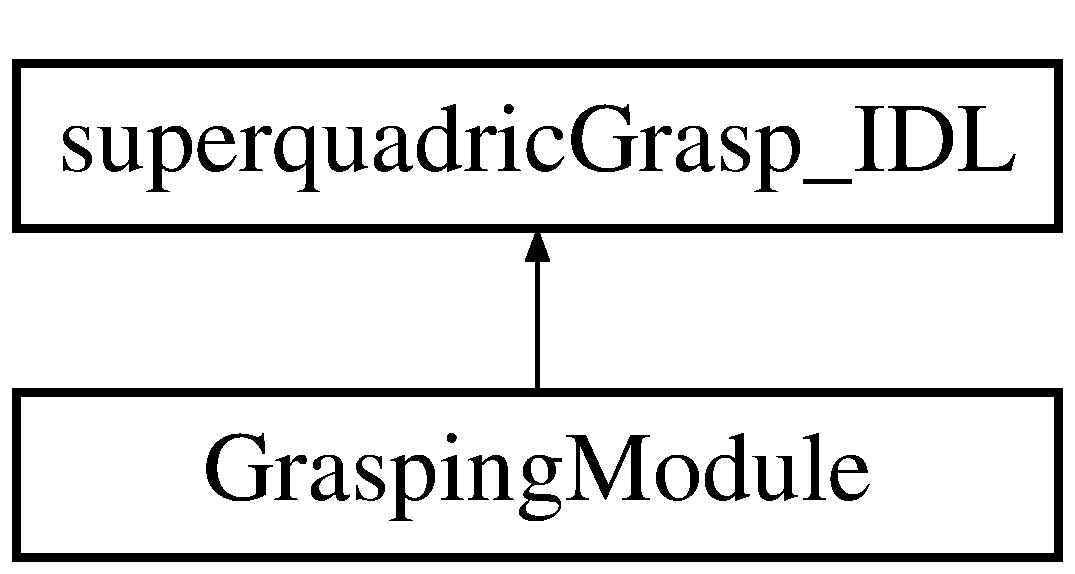
\includegraphics[height=2.000000cm]{classGraspingModule}
\end{center}
\end{figure}
\subsection*{Public Member Functions}
\begin{DoxyCompactItemize}
\item 
bool {\bfseries attach} (yarp\+::os\+::\+Rpc\+Server \&source)\label{classGraspingModule_ac3e7a265105f99952742a6aca17d67c3}

\item 
std\+::string \hyperlink{classGraspingModule_aabedec650875263d27ecf20fa9dd8b39}{get\+\_\+visualization} ()
\begin{DoxyCompactList}\small\item\em Return if visualization is on or off. \end{DoxyCompactList}\item 
bool \hyperlink{classGraspingModule_a801de4b63aba360a4b85e322c5947a4a}{set\+\_\+visualization} (const std\+::string \&e)
\begin{DoxyCompactList}\small\item\em Set visualization option on or off. \end{DoxyCompactList}\item 
std\+::string \hyperlink{classGraspingModule_a5103f8bd6671a11a9bd1c7e29d290009}{get\+\_\+best\+\_\+hand} ()
\begin{DoxyCompactList}\small\item\em Return the computed grasping poses. \end{DoxyCompactList}\item 
yarp\+::os\+::\+Property \hyperlink{classGraspingModule_af1e057f767ab83be185cf486d3f5c46b}{get\+\_\+grasping\+\_\+pose} (const yarp\+::os\+::\+Property \&superquadric, const std\+::string \&\hyperlink{classGraspingModule_af8308a8938957b4bb50c260dc42d7b27}{hand})
\begin{DoxyCompactList}\small\item\em Return the estimated grasping poses given an estimated superquadric. \end{DoxyCompactList}\item 
yarp\+::os\+::\+Property \hyperlink{classGraspingModule_a375475691c644d8aa882db8d65ceda50}{get\+\_\+options} (const std\+::string \&field)
\begin{DoxyCompactList}\small\item\em Get options of the field of interest. \end{DoxyCompactList}\item 
bool \hyperlink{classGraspingModule_a849c459ef9700c93b45ef6cff394f675}{set\+\_\+options} (const yarp\+::os\+::\+Property \&new\+Options, const std\+::string \&field)
\begin{DoxyCompactList}\small\item\em Set options of the field of interest. \end{DoxyCompactList}\item 
std\+::string \hyperlink{classGraspingModule_a557a87131c7396dd62c02eced7f4a937}{get\+\_\+hand} ()
\begin{DoxyCompactList}\small\item\em Return which hand has been enabled. \end{DoxyCompactList}\item 
bool \hyperlink{classGraspingModule_a9d34cb0521f86dd16648255e640eec90}{set\+\_\+hand} (const std\+::string \&e)
\begin{DoxyCompactList}\small\item\em Set hand enabled. \end{DoxyCompactList}\item 
bool \hyperlink{classGraspingModule_a618785dec349358760a05e6e4b097866}{set\+\_\+save\+\_\+poses} (const std\+::string \&entry)
\begin{DoxyCompactList}\small\item\em Return if poses are saved or not. \end{DoxyCompactList}\item 
std\+::string \hyperlink{classGraspingModule_a949e4297bdf26f564669ffc91068c4f3}{get\+\_\+save\+\_\+poses} ()
\begin{DoxyCompactList}\small\item\em Set if poses are saved or not. \end{DoxyCompactList}\item 
yarp\+::os\+::\+Property \hyperlink{classGraspingModule_a059da011f804acd1adc4549eaa3d2141}{fill\+Property} (const yarp\+::sig\+::\+Vector \&sol)
\begin{DoxyCompactList}\small\item\em Fill property with the grasping solutions. \end{DoxyCompactList}\item 
bool \hyperlink{classGraspingModule_a834e972a2a1b7b92bf8dc1e83319b028}{clear\+\_\+poses} ()
\begin{DoxyCompactList}\small\item\em Delete computed poses. \end{DoxyCompactList}\item 
bool \hyperlink{classGraspingModule_a08bd9cdbb1d16da8616c9769510e2bf1}{move} (const std\+::string \&entry)
\begin{DoxyCompactList}\small\item\em Move the selected arm. \end{DoxyCompactList}\item 
bool \hyperlink{classGraspingModule_a518ee4ec1b27d32c600f340c0f3bf552}{config\+Basics} (yarp\+::os\+::\+Resource\+Finder \&rf)
\begin{DoxyCompactList}\small\item\em Configure basics options. \end{DoxyCompactList}\item 
bool \hyperlink{classGraspingModule_a151b46117f2d1fdd8c321554012d63f3}{close} ()
\begin{DoxyCompactList}\small\item\em Close function of the RF module. \end{DoxyCompactList}\item 
bool \hyperlink{classGraspingModule_aca7dc9ec5e0a98b1333ed4c63650cdba}{interrupt\+Module} ()
\begin{DoxyCompactList}\small\item\em Interrupt function of the RF module. \end{DoxyCompactList}\item 
bool \hyperlink{classGraspingModule_af2cd7fa157b5d78080ffd7952655046d}{update\+Module} ()
\begin{DoxyCompactList}\small\item\em Update function of the RF module. \end{DoxyCompactList}\item 
double \hyperlink{classGraspingModule_abfc60b8437d750f2b2a48b8a617e53c1}{get\+Period} ()
\begin{DoxyCompactList}\small\item\em Get period function of the RF module. \end{DoxyCompactList}\item 
bool \hyperlink{classGraspingModule_a1086203a4db1e465ef8aba5e28f60025}{config\+Viewer} (yarp\+::os\+::\+Resource\+Finder \&rf)
\begin{DoxyCompactList}\small\item\em Configure options for visualization. \end{DoxyCompactList}\item 
bool \hyperlink{classGraspingModule_ab6d6d4c684340a0e4988a338ff72e3d0}{config\+Pose} (yarp\+::os\+::\+Resource\+Finder \&rf)
\begin{DoxyCompactList}\small\item\em Configure options for pose computation. \end{DoxyCompactList}\item 
bool \hyperlink{classGraspingModule_af83c4dc5cdc8ed18a03ce2637abda2e9}{config\+Movements} (yarp\+::os\+::\+Resource\+Finder \&rf)
\begin{DoxyCompactList}\small\item\em Configure options for arm movements. \end{DoxyCompactList}\item 
bool \hyperlink{classGraspingModule_a31c82e1ba3c80d1238e95449780f62c6}{config\+Grasp} (yarp\+::os\+::\+Resource\+Finder \&rf)
\begin{DoxyCompactList}\small\item\em Configure options for grasping. \end{DoxyCompactList}\item 
bool \hyperlink{classGraspingModule_ab4c0ea3cabb2cc6de63da53ba1771e27}{configure} (yarp\+::os\+::\+Resource\+Finder \&rf)\label{classGraspingModule_ab4c0ea3cabb2cc6de63da53ba1771e27}

\begin{DoxyCompactList}\small\item\em Configure function of RF module. \end{DoxyCompactList}\item 
bool \hyperlink{classGraspingModule_aa1c32186a8b7133db63e115898949b28}{read\+Superq} (const std\+::string \&name\+\_\+obj, yarp\+::sig\+::\+Vector \&x, const int \&dimension, yarp\+::os\+::\+Resource\+Finder $\ast$rf)
\begin{DoxyCompactList}\small\item\em Read object model from text file for simulation tests. \end{DoxyCompactList}\item 
void \hyperlink{classGraspingModule_a43a89c97919dd68a4ab28a6c9fe16a95}{save\+Sol} (const yarp\+::os\+::\+Property \&sol)
\begin{DoxyCompactList}\small\item\em Save solutions. \end{DoxyCompactList}\item 
bool {\bfseries look\+\_\+center} ()\label{classGraspingModule_af640219e03fdfe6e6145a5ff6f01d23a}

\item 
bool {\bfseries look\+\_\+obj} ()\label{classGraspingModule_a741cac4968db05d8dde9cd1856776c50}

\item 
bool \hyperlink{classGraspingModule_a1455fc4c6a1ae5690fa691cc324fec4e}{go\+\_\+home} (const std\+::string \&entry)
\begin{DoxyCompactList}\small\item\em Go back to home position. \end{DoxyCompactList}\item 
bool \hyperlink{classGraspingModule_a75482819f7f289b3f456571628952122}{go\+\_\+to\+\_\+basket} (const std\+::string \&entry)
\begin{DoxyCompactList}\small\item\em Go back to the basket on the robot side. \end{DoxyCompactList}\item 
bool \hyperlink{classGraspingModule_a91eac72e632f224442f34b907e479fa3}{check\+\_\+motion} ()
\begin{DoxyCompactList}\small\item\em Check if the motion has been completed. \end{DoxyCompactList}\item 
bool \hyperlink{classGraspingModule_a650c026153e3a7b0044f508cf9d4bf00}{check\+\_\+home} ()
\begin{DoxyCompactList}\small\item\em Check if the motion back to home has been completed. \end{DoxyCompactList}\item 
bool \hyperlink{classGraspingModule_a19ee1967a83d1412f9125ec482ce80bd}{check\+\_\+basket} ()
\begin{DoxyCompactList}\small\item\em Check if the motion to the basket has been completed. \end{DoxyCompactList}\item 
virtual bool \hyperlink{classsuperquadricGrasp__IDL_ac40ef7c0dd4f0e3600db9aea5cc5c298}{calibrate} ()
\begin{DoxyCompactList}\small\item\em Calibrate plane height via superquadric computation. \end{DoxyCompactList}\item 
virtual bool {\bfseries read} (yarp\+::os\+::\+Connection\+Reader \&connection) Y\+A\+R\+P\+\_\+\+O\+V\+E\+R\+R\+I\+DE\label{classsuperquadricGrasp__IDL_a710271cfee0c9b1a31707d84f194b69b}

\item 
virtual std\+::vector$<$ std\+::string $>$ {\bfseries help} (const std\+::string \&function\+Name=\char`\"{}-\/-\/all\char`\"{})\label{classsuperquadricGrasp__IDL_a226f766d3a3a0ba87e7c1fa0aceb2cb8}

\end{DoxyCompactItemize}
\subsection*{Protected Attributes}
\begin{DoxyCompactItemize}
\item 
yarp\+::os\+::\+Resource\+Finder $\ast$ {\bfseries rf}\label{classGraspingModule_aed592146c8031a537a8d1f71a7e054c5}

\item 
std\+::string \hyperlink{classGraspingModule_a508cc33e7003b294f00316f362f82eaa}{robot}\label{classGraspingModule_a508cc33e7003b294f00316f362f82eaa}

\begin{DoxyCompactList}\small\item\em Robot name\+: icub or icub\+Sim. \end{DoxyCompactList}\item 
std\+::string \hyperlink{classGraspingModule_ab9603885e438ebe5a7f673c04bc37ed8}{left\+\_\+or\+\_\+right}\label{classGraspingModule_ab9603885e438ebe5a7f673c04bc37ed8}

\begin{DoxyCompactList}\small\item\em Hand to be enabled with the code. \end{DoxyCompactList}\item 
std\+::string \hyperlink{classGraspingModule_a0aa116f84336b88479b6f3ac6a97e76b}{home\+Context\+Path}\label{classGraspingModule_a0aa116f84336b88479b6f3ac6a97e76b}

\begin{DoxyCompactList}\small\item\em Path where the context is imported. \end{DoxyCompactList}\item 
yarp\+::sig\+::\+Vector \hyperlink{classGraspingModule_ae819bea3ec49cbec2703737a7a786007}{poseL}\label{classGraspingModule_ae819bea3ec49cbec2703737a7a786007}

\begin{DoxyCompactList}\small\item\em Robot hand pose computed by the solver for the left hand. \end{DoxyCompactList}\item 
yarp\+::sig\+::\+Vector \hyperlink{classGraspingModule_a0a13dee5ac1b2db61a87f82ecdc44ea6}{solL}\label{classGraspingModule_a0a13dee5ac1b2db61a87f82ecdc44ea6}

\begin{DoxyCompactList}\small\item\em Hand ellipsoid pose computed by the solver for the left hand. \end{DoxyCompactList}\item 
yarp\+::sig\+::\+Vector \hyperlink{classGraspingModule_a148c46809e3dba05972df158c81c48f8}{poseR}\label{classGraspingModule_a148c46809e3dba05972df158c81c48f8}

\begin{DoxyCompactList}\small\item\em Robot hand pose computed by the solver for the right hand. \end{DoxyCompactList}\item 
yarp\+::sig\+::\+Vector \hyperlink{classGraspingModule_a1215352771f0e7f26e033ad95731a81e}{solR}\label{classGraspingModule_a1215352771f0e7f26e033ad95731a81e}

\begin{DoxyCompactList}\small\item\em Hand ellipsoid pose computed by the solver for the right hand. \end{DoxyCompactList}\item 
std\+::deque$<$ yarp\+::sig\+::\+Vector $>$ \hyperlink{classGraspingModule_ac7c1f1dc2e81ed15f87218feaa038988}{trajectory\+\_\+right}\label{classGraspingModule_ac7c1f1dc2e81ed15f87218feaa038988}

\begin{DoxyCompactList}\small\item\em Entire trajectory (final pose and waypoint) for the right hand. \end{DoxyCompactList}\item 
std\+::deque$<$ yarp\+::sig\+::\+Vector $>$ \hyperlink{classGraspingModule_afcfe41fdc6ce4446e89594a3d40d2a7d}{trajectory\+\_\+left}\label{classGraspingModule_afcfe41fdc6ce4446e89594a3d40d2a7d}

\begin{DoxyCompactList}\small\item\em Entire trajectory (final pose and waypoint) for the left hand. \end{DoxyCompactList}\item 
int \hyperlink{classGraspingModule_ab87532f4790da036cdf51654a649cece}{context\+\_\+gaze}\label{classGraspingModule_ab87532f4790da036cdf51654a649cece}

\begin{DoxyCompactList}\small\item\em Variable for saving gaze context. \end{DoxyCompactList}\item 
int \hyperlink{classGraspingModule_a26e3aee1196f9b3783426f5be6a387b5}{rate\+\_\+vis}\label{classGraspingModule_a26e3aee1196f9b3783426f5be6a387b5}

\begin{DoxyCompactList}\small\item\em Rate of the visualization thread. \end{DoxyCompactList}\item 
int \hyperlink{classGraspingModule_a244cb8f6f2b2294d2be164ee1518cc36}{print\+\_\+level}\label{classGraspingModule_a244cb8f6f2b2294d2be164ee1518cc36}

\begin{DoxyCompactList}\small\item\em Print level for the Ipopt optimization problem. \end{DoxyCompactList}\item 
double {\bfseries t}\label{classGraspingModule_a4f36c3ca4e343f62ec908768af45a3da}

\item 
double {\bfseries t0}\label{classGraspingModule_a70a4e9c60616c7e7c63b11594e73a6ac}

\item 
double {\bfseries t\+\_\+grasp}\label{classGraspingModule_aaf674331d6bbf84ea008566948c6dee2}

\item 
double {\bfseries t\+\_\+vis}\label{classGraspingModule_ae0cddf0f4c4e7d00197a1c45ff98f0e5}

\item 
std\+::deque$<$ double $>$ {\bfseries times\+\_\+vis}\label{classGraspingModule_a9a0dedfb6b400af32cd04a9eafd43dba}

\item 
double \hyperlink{classGraspingModule_a521b7c66535fb4dac516a9ff58241f05}{tol}\label{classGraspingModule_a521b7c66535fb4dac516a9ff58241f05}

\begin{DoxyCompactList}\small\item\em Tolerance of the Ipopt optimization problem. \end{DoxyCompactList}\item 
int \hyperlink{classGraspingModule_a3f17b0601f067499b5f574fb8c6f937e}{max\+\_\+iter}\label{classGraspingModule_a3f17b0601f067499b5f574fb8c6f937e}

\begin{DoxyCompactList}\small\item\em Maximum iteration allowed for the Ipopt optimization problem. \end{DoxyCompactList}\item 
int \hyperlink{classGraspingModule_aa4dff98eeb8125bc88613b15159cd26c}{n\+\_\+pointshand}\label{classGraspingModule_aa4dff98eeb8125bc88613b15159cd26c}

\begin{DoxyCompactList}\small\item\em Number of points sampled on the hand ellipsoid for the Ipopt optimization problem. \end{DoxyCompactList}\item 
int \hyperlink{classGraspingModule_ab3821aa16b5021be595ac8b7db4d6cfb}{acceptable\+\_\+iter}\label{classGraspingModule_ab3821aa16b5021be595ac8b7db4d6cfb}

\begin{DoxyCompactList}\small\item\em Acceptable iter of the Ipopt optimization problem. \end{DoxyCompactList}\item 
double \hyperlink{classGraspingModule_a5529bf668b7ea95582ea238d5f50e3c2}{constr\+\_\+viol\+\_\+tol}\label{classGraspingModule_a5529bf668b7ea95582ea238d5f50e3c2}

\begin{DoxyCompactList}\small\item\em Constraint tolerance of the Ipopt optimization problem. \end{DoxyCompactList}\item 
std\+::string \hyperlink{classGraspingModule_a64763408867f3cb6dc508c91f8cf220a}{mu\+\_\+strategy}\label{classGraspingModule_a64763408867f3cb6dc508c91f8cf220a}

\begin{DoxyCompactList}\small\item\em Mu strategy of the Ipopt optimization problem. \end{DoxyCompactList}\item 
std\+::string \hyperlink{classGraspingModule_aecc5738f9012849c9edaf35f479723b4}{nlp\+\_\+scaling\+\_\+method}\label{classGraspingModule_aecc5738f9012849c9edaf35f479723b4}

\begin{DoxyCompactList}\small\item\em N\+LP scaling method of the Ipopt optimization problem. \end{DoxyCompactList}\item 
double \hyperlink{classGraspingModule_a3dabf2eac967efb30b1b7bb9c91e41b3}{max\+\_\+cpu\+\_\+time}\label{classGraspingModule_a3dabf2eac967efb30b1b7bb9c91e41b3}

\begin{DoxyCompactList}\small\item\em Max cpu time allowed for the Ipopt optimization problem. \end{DoxyCompactList}\item 
std\+::string \hyperlink{classGraspingModule_a87c885eada6df4d622c92173d8a4ed2e}{dir}
\begin{DoxyCompactList}\small\item\em Direction for generating the waypoint for the approach\+: it could be on x and z axes (\char`\"{}xz\char`\"{}) or only z axis (\char`\"{}z\char`\"{}) of the hand reference frame. \end{DoxyCompactList}\item 
yarp\+::sig\+::\+Vector \hyperlink{classGraspingModule_a4b3ada8a9325ed821e73b8e84375c4fa}{object}\label{classGraspingModule_a4b3ada8a9325ed821e73b8e84375c4fa}

\begin{DoxyCompactList}\small\item\em Object superquadric. \end{DoxyCompactList}\item 
yarp\+::sig\+::\+Vector \hyperlink{classGraspingModule_af8308a8938957b4bb50c260dc42d7b27}{hand}\label{classGraspingModule_af8308a8938957b4bb50c260dc42d7b27}

\begin{DoxyCompactList}\small\item\em Hand ellipsoid for the first hand enabled. \end{DoxyCompactList}\item 
yarp\+::sig\+::\+Vector \hyperlink{classGraspingModule_a0b4986d666ef55b1c769d1b02b49c86f}{hand1}\label{classGraspingModule_a0b4986d666ef55b1c769d1b02b49c86f}

\begin{DoxyCompactList}\small\item\em Hand ellipsoid for the second hand enabled. \end{DoxyCompactList}\item 
double \hyperlink{classGraspingModule_af1912ddc2800fb3101e98a99d3b04b5b}{distance}\label{classGraspingModule_af1912ddc2800fb3101e98a99d3b04b5b}

\begin{DoxyCompactList}\small\item\em Distance for shifting the waypoint along x axis of the hand reference frame. \end{DoxyCompactList}\item 
double \hyperlink{classGraspingModule_aacb0581ba76204e825aee632cf9679e4}{distance1}\label{classGraspingModule_aacb0581ba76204e825aee632cf9679e4}

\begin{DoxyCompactList}\small\item\em Distance for shifting the waypoint along z axis of the hand reference frame. \end{DoxyCompactList}\item 
yarp\+::sig\+::\+Vector \hyperlink{classGraspingModule_a52131b73f3688ab8524f37b8e1945717}{displacement}\label{classGraspingModule_a52131b73f3688ab8524f37b8e1945717}

\begin{DoxyCompactList}\small\item\em Distance of the robot pose with respect to the hand ellipsoid along x axis of the hand reference frame. \end{DoxyCompactList}\item 
yarp\+::sig\+::\+Vector \hyperlink{classGraspingModule_a234e3ab635ba9b581e6877519dc633b6}{plane}\label{classGraspingModule_a234e3ab635ba9b581e6877519dc633b6}

\begin{DoxyCompactList}\small\item\em Parameters of the implicit function describing the plane on which the object is located in the root reference frame. \end{DoxyCompactList}\item 
yarp\+::os\+::\+Rpc\+Server \hyperlink{classGraspingModule_a164dc4c91253669941ad45e2702bb746}{port\+Rpc}\label{classGraspingModule_a164dc4c91253669941ad45e2702bb746}

\begin{DoxyCompactList}\small\item\em Rpc port for services. \end{DoxyCompactList}\item 
std\+::string \hyperlink{classGraspingModule_a2d764f516aecffb52ba22f1dcdd2a730}{eye}\label{classGraspingModule_a2d764f516aecffb52ba22f1dcdd2a730}

\begin{DoxyCompactList}\small\item\em Eye camera selected for visualization. \end{DoxyCompactList}\item 
double \hyperlink{classGraspingModule_a9562cc675af9a861201956fe23a267bc}{block\+\_\+eye}\label{classGraspingModule_a9562cc675af9a861201956fe23a267bc}

\begin{DoxyCompactList}\small\item\em Vergence value for blocking the eyes. \end{DoxyCompactList}\item 
double \hyperlink{classGraspingModule_aa92c21ad6a4a5f70f73ebf3281676f62}{block\+\_\+neck}\label{classGraspingModule_aa92c21ad6a4a5f70f73ebf3281676f62}

\begin{DoxyCompactList}\small\item\em Neck joint value for looking to the table. \end{DoxyCompactList}\item 
yarp\+::sig\+::\+Matrix {\bfseries K}\label{classGraspingModule_a161a8c4d8bc2db6e1cf7c00a69953831}

\item 
yarp\+::sig\+::\+Matrix {\bfseries H}\label{classGraspingModule_acb55c5d37d9a7225b44323d2be724bfe}

\item 
yarp\+::dev\+::\+Poly\+Driver {\bfseries Gaze\+Ctrl}\label{classGraspingModule_adfed9afcb5290a5ee2e99768352fd4fb}

\item 
yarp\+::dev\+::\+I\+Gaze\+Control $\ast$ {\bfseries igaze}\label{classGraspingModule_a70a410aead666d7198eb183ba05472a5}

\item 
std\+::string {\bfseries fing}\label{classGraspingModule_ad33afeaa6a6b67f3f49ccb4ee771e6cb}

\item 
bool \hyperlink{classGraspingModule_ae7f23202919c7dbd742230a2cc005043}{lift\+\_\+object}\label{classGraspingModule_ae7f23202919c7dbd742230a2cc005043}

\begin{DoxyCompactList}\small\item\em Boolean variable to lift or not the object. \end{DoxyCompactList}\item 
std\+::string {\bfseries lobj}\label{classGraspingModule_af871b2ab1e5110408893eef5ac711984}

\item 
bool \hyperlink{classGraspingModule_aa1da1c0d76de383f74360bc9c9125e77}{go\+\_\+on}\label{classGraspingModule_aa1da1c0d76de383f74360bc9c9125e77}

\begin{DoxyCompactList}\small\item\em Boolean variable used for going to the next step of the state machine. \end{DoxyCompactList}\item 
bool \hyperlink{classGraspingModule_ae56f0d9a9eed5d68051da744dac15a41}{grasp}\label{classGraspingModule_ae56f0d9a9eed5d68051da744dac15a41}

\begin{DoxyCompactList}\small\item\em Boolean variable to grasp or not the object. \end{DoxyCompactList}\item 
bool \hyperlink{classGraspingModule_a499af38a89686312a34117c0218fc6cb}{executed}\label{classGraspingModule_a499af38a89686312a34117c0218fc6cb}

\begin{DoxyCompactList}\small\item\em Boolean variable taking into account if the movement has been executed. \end{DoxyCompactList}\item 
bool \hyperlink{classGraspingModule_abdcf071d6ce460a83c56ef1ba90f8b1f}{executed\+\_\+var}\label{classGraspingModule_abdcf071d6ce460a83c56ef1ba90f8b1f}

\begin{DoxyCompactList}\small\item\em Boolean variable taking into account if the movement has been executed (for different checks) \end{DoxyCompactList}\item 
bool \hyperlink{classGraspingModule_af46e9f6a4a79bb39db0f975803d739b3}{reached\+\_\+home}\label{classGraspingModule_af46e9f6a4a79bb39db0f975803d739b3}

\begin{DoxyCompactList}\small\item\em Boolean variable taking into account if the home pose has been reached. \end{DoxyCompactList}\item 
bool \hyperlink{classGraspingModule_a295ffc6e5c40dea6d6e222f3f487ec67}{reached\+\_\+basket}\label{classGraspingModule_a295ffc6e5c40dea6d6e222f3f487ec67}

\begin{DoxyCompactList}\small\item\em Boolean variable taking into account if the basket pose has been reached. \end{DoxyCompactList}\item 
std\+::string \hyperlink{classGraspingModule_af05d3fc99e87d5ab513bb9fe91f0bcea}{show\+\_\+hand}\label{classGraspingModule_af05d3fc99e87d5ab513bb9fe91f0bcea}

\begin{DoxyCompactList}\small\item\em String variable for showing (on) or not (off) the hand ellipsoid on the viewer. \end{DoxyCompactList}\item 
std\+::string \hyperlink{classGraspingModule_ae9a9a1e59ba2298fac3c4f34996ec25e}{show\+\_\+only\+\_\+pose}\label{classGraspingModule_ae9a9a1e59ba2298fac3c4f34996ec25e}

\begin{DoxyCompactList}\small\item\em String variable for showing only the final pose(on) or also the trajectory (off) on the viewer. \end{DoxyCompactList}\item 
std\+::string \hyperlink{classGraspingModule_ac74a028982f21c24a3405deb41e70f9f}{look\+\_\+object}\label{classGraspingModule_ac74a028982f21c24a3405deb41e70f9f}

\begin{DoxyCompactList}\small\item\em String variable for fixating at the object (on) or not (off) during movements. \end{DoxyCompactList}\item 
bool \hyperlink{classGraspingModule_afb42ea3b2951d1e8abe7f391675d8f73}{visualization}\label{classGraspingModule_afb42ea3b2951d1e8abe7f391675d8f73}

\begin{DoxyCompactList}\small\item\em Boolean variable for enabling visualization. \end{DoxyCompactList}\item 
bool \hyperlink{classGraspingModule_afa54033aed276e29223d9a88a6f7f145}{mode\+\_\+online}\label{classGraspingModule_afa54033aed276e29223d9a88a6f7f145}

\begin{DoxyCompactList}\small\item\em Boolean variable for switching between online and offline mode. \end{DoxyCompactList}\item 
bool \hyperlink{classGraspingModule_a8193f9e7fc2e65f52bf80580735113bc}{save\+\_\+poses}\label{classGraspingModule_a8193f9e7fc2e65f52bf80580735113bc}

\begin{DoxyCompactList}\small\item\em String variable for saving the solutions. \end{DoxyCompactList}\item 
bool {\bfseries also\+\_\+traj}\label{classGraspingModule_ada586ca7d90ea75cf6be9847ddb274c7}

\item 
double \hyperlink{classGraspingModule_abd2e8eaca9dd18e74a40fd3831922c16}{force\+\_\+threshold}
\begin{DoxyCompactList}\small\item\em Threshold of the maximum allowed force measured at the endeffector. \end{DoxyCompactList}\item 
std\+::string \hyperlink{classGraspingModule_ad74775f47ff255bde51b0bab79a31728}{compliant}\label{classGraspingModule_ad74775f47ff255bde51b0bab79a31728}

\begin{DoxyCompactList}\small\item\em String variable for enabling the compliant mode. \end{DoxyCompactList}\item 
std\+::string \hyperlink{classGraspingModule_a79082a891f887dbb9edfed4653451e35}{visual\+\_\+servoing}\label{classGraspingModule_a79082a891f887dbb9edfed4653451e35}

\begin{DoxyCompactList}\small\item\em String variable for the visual servoing controller during the final pose reaching. \end{DoxyCompactList}\item 
std\+::string \hyperlink{classGraspingModule_a832c738961170cb80a024805b22464b8}{use\+\_\+direct\+\_\+kin}\label{classGraspingModule_a832c738961170cb80a024805b22464b8}

\begin{DoxyCompactList}\small\item\em String variable for using visual servoing with direct kinematics, instead of hand pose estimate. \end{DoxyCompactList}\item 
double \hyperlink{classGraspingModule_aa84058eee1411f35aa489b9cad9f9371}{pixel\+\_\+tol}\label{classGraspingModule_aa84058eee1411f35aa489b9cad9f9371}

\begin{DoxyCompactList}\small\item\em Pixel tolerance for visual servoing. \end{DoxyCompactList}\item 
double \hyperlink{classGraspingModule_a676c7aa895de03ba5362a309cd669905}{lift\+\_\+z}\label{classGraspingModule_a676c7aa895de03ba5362a309cd669905}

\begin{DoxyCompactList}\small\item\em How much the robot should lift the object. \end{DoxyCompactList}\item 
double \hyperlink{classGraspingModule_af1feeb0f4397d83491831327e05c8b44}{torso\+\_\+pitch\+\_\+max}\label{classGraspingModule_af1feeb0f4397d83491831327e05c8b44}

\begin{DoxyCompactList}\small\item\em Maximum pitch value for avoiding movements to close to the table while reaching some particular poses. \end{DoxyCompactList}\item 
double \hyperlink{classGraspingModule_a02accb5392fe0877a2a98febbcf20ea6}{traj\+\_\+time}\label{classGraspingModule_a02accb5392fe0877a2a98febbcf20ea6}

\begin{DoxyCompactList}\small\item\em Time for reaching each waypoint of the trajectory. \end{DoxyCompactList}\item 
double \hyperlink{classGraspingModule_a2b59e1c09ae51bb1829cb4b73799a9d2}{traj\+\_\+tol}\label{classGraspingModule_a2b59e1c09ae51bb1829cb4b73799a9d2}

\begin{DoxyCompactList}\small\item\em Reaching tolerance for the cartesian. \end{DoxyCompactList}\item 
yarp\+::sig\+::\+Vector \hyperlink{classGraspingModule_a589b2e394e0d255fcd23734b911392ef}{shift\+\_\+right}\label{classGraspingModule_a589b2e394e0d255fcd23734b911392ef}

\begin{DoxyCompactList}\small\item\em 3D shift for the final right pose along x, y, and z axes of the right hand reference frame for compensating with eye-\/kinematics offsets \end{DoxyCompactList}\item 
yarp\+::sig\+::\+Vector \hyperlink{classGraspingModule_a96feca3ff9d44e599351ddb1c4497fcf}{shift\+\_\+left}\label{classGraspingModule_a96feca3ff9d44e599351ddb1c4497fcf}

\begin{DoxyCompactList}\small\item\em 3D shift for the final left pose along x, y, and z axes of the left hand reference frame for compensating with eye-\/kinematics offsets \end{DoxyCompactList}\item 
yarp\+::sig\+::\+Vector \hyperlink{classGraspingModule_ac43f827abab558d8aea39a6cbcd150a2}{home\+\_\+right}\label{classGraspingModule_ac43f827abab558d8aea39a6cbcd150a2}

\begin{DoxyCompactList}\small\item\em Home pose (7D) for the right hand. \end{DoxyCompactList}\item 
yarp\+::sig\+::\+Vector \hyperlink{classGraspingModule_a75a4689473261072a85c67c76ac6567f}{home\+\_\+left}\label{classGraspingModule_a75a4689473261072a85c67c76ac6567f}

\begin{DoxyCompactList}\small\item\em Home pose (7D) for the left hand. \end{DoxyCompactList}\item 
yarp\+::sig\+::\+Vector \hyperlink{classGraspingModule_a514ee9d4045d3e551a089ffd1f296c49}{basket\+\_\+right}\label{classGraspingModule_a514ee9d4045d3e551a089ffd1f296c49}

\begin{DoxyCompactList}\small\item\em Basket pose (7D) for the right hand. \end{DoxyCompactList}\item 
yarp\+::sig\+::\+Vector \hyperlink{classGraspingModule_a4c2cf37b608df9bdce4ff5a2882111ef}{basket\+\_\+left}\label{classGraspingModule_a4c2cf37b608df9bdce4ff5a2882111ef}

\begin{DoxyCompactList}\small\item\em Basket pose (7D) for the left hand. \end{DoxyCompactList}\item 
yarp\+::sig\+::\+Vector \hyperlink{classGraspingModule_af25aefd74e3a455cd3288896dc7f545e}{stiff\+\_\+right}\label{classGraspingModule_af25aefd74e3a455cd3288896dc7f545e}

\begin{DoxyCompactList}\small\item\em Stiff values for the right hand. \end{DoxyCompactList}\item 
yarp\+::sig\+::\+Vector \hyperlink{classGraspingModule_a39f2ad508bb3f5baeac30684cd57bf44}{stiff\+\_\+left}\label{classGraspingModule_a39f2ad508bb3f5baeac30684cd57bf44}

\begin{DoxyCompactList}\small\item\em Stiff values for the left hand. \end{DoxyCompactList}\item 
yarp\+::sig\+::\+Vector \hyperlink{classGraspingModule_af7690eeb0850a02dc05e20e4c4326dd4}{damp\+\_\+right}\label{classGraspingModule_af7690eeb0850a02dc05e20e4c4326dd4}

\begin{DoxyCompactList}\small\item\em Damp values for the right hand. \end{DoxyCompactList}\item 
yarp\+::sig\+::\+Vector \hyperlink{classGraspingModule_ad4dda6219b8a0bf9636c7bf58effc14b}{damp\+\_\+left}\label{classGraspingModule_ad4dda6219b8a0bf9636c7bf58effc14b}

\begin{DoxyCompactList}\small\item\em Damp values for the left hand. \end{DoxyCompactList}\item 
std\+::string \hyperlink{classGraspingModule_af119be2a7acbb0568d1c08f4f6069928}{hand\+\_\+to\+\_\+move}\label{classGraspingModule_af119be2a7acbb0568d1c08f4f6069928}

\begin{DoxyCompactList}\small\item\em Hand selected for grasping the object. \end{DoxyCompactList}\item 
std\+::string \hyperlink{classGraspingModule_a627ae74edcebd1e63427d1923bf07004}{name\+File\+Out\+\_\+right}\label{classGraspingModule_a627ae74edcebd1e63427d1923bf07004}

\begin{DoxyCompactList}\small\item\em File name of Ipopt output for right hand. \end{DoxyCompactList}\item 
std\+::string \hyperlink{classGraspingModule_a2d67456b32002aeca338be1844e5fe79}{name\+File\+Trajectory\+\_\+right}\label{classGraspingModule_a2d67456b32002aeca338be1844e5fe79}

\begin{DoxyCompactList}\small\item\em File name containing trajectory for right hand. \end{DoxyCompactList}\item 
std\+::string \hyperlink{classGraspingModule_a3d16b71a4e021206b2b60dca65b6bf88}{name\+File\+Out\+\_\+left}\label{classGraspingModule_a3d16b71a4e021206b2b60dca65b6bf88}

\begin{DoxyCompactList}\small\item\em File name of Ipopt output for left hand. \end{DoxyCompactList}\item 
std\+::string \hyperlink{classGraspingModule_a1f3841076509b5140edbdb7d01aa3f4b}{name\+File\+Trajectory\+\_\+left}\label{classGraspingModule_a1f3841076509b5140edbdb7d01aa3f4b}

\begin{DoxyCompactList}\small\item\em File name containing trajectory for left hand. \end{DoxyCompactList}\item 
std\+::string \hyperlink{classGraspingModule_a7d96e2271d553a340888ffa1a422d608}{lib\+\_\+context}\label{classGraspingModule_a7d96e2271d553a340888ffa1a422d608}

\begin{DoxyCompactList}\small\item\em Context name for the module for closing the fingers. \end{DoxyCompactList}\item 
std\+::string \hyperlink{classGraspingModule_a437d621f1b6e1ce0d5cc1d8958b53fee}{lib\+\_\+filename}\label{classGraspingModule_a437d621f1b6e1ce0d5cc1d8958b53fee}

\begin{DoxyCompactList}\small\item\em File name of the module used for closing the fingers. \end{DoxyCompactList}\item 
yarp\+::os\+::\+Mutex {\bfseries mutex}\label{classGraspingModule_ae27bf275f6a5f99728586ae235477683}

\item 
\hyperlink{classGraspComputation}{Grasp\+Computation} $\ast$ \hyperlink{classGraspingModule_a2a88d576e1cc46c209d6ff40657f1ddb}{grasp\+Comp}\label{classGraspingModule_a2a88d576e1cc46c209d6ff40657f1ddb}

\begin{DoxyCompactList}\small\item\em Class computing the grasping pose. \end{DoxyCompactList}\item 
\hyperlink{classGraspVisualization}{Grasp\+Visualization} $\ast$ \hyperlink{classGraspingModule_a98acb57493a68c3ce14f6e89b721aa23}{grasp\+Vis}\label{classGraspingModule_a98acb57493a68c3ce14f6e89b721aa23}

\begin{DoxyCompactList}\small\item\em Class showing the grasping pose on the viewer. \end{DoxyCompactList}\item 
\hyperlink{classGraspExecution}{Grasp\+Execution} $\ast$ \hyperlink{classGraspingModule_a1c5e0b94e7b086d14ac1bf45db3007f1}{grasp\+Exec}\label{classGraspingModule_a1c5e0b94e7b086d14ac1bf45db3007f1}

\begin{DoxyCompactList}\small\item\em Class executing the trajectory. \end{DoxyCompactList}\item 
yarp\+::os\+::\+Property \hyperlink{classGraspingModule_a2d8f2bb7d5263b2df89d7431fe830525}{vis\+\_\+par}\label{classGraspingModule_a2d8f2bb7d5263b2df89d7431fe830525}

\begin{DoxyCompactList}\small\item\em Parameters of the visualization class. \end{DoxyCompactList}\item 
yarp\+::os\+::\+Property \hyperlink{classGraspingModule_ac5132578e072a0cd851a888487d4e144}{pose\+\_\+par}\label{classGraspingModule_ac5132578e072a0cd851a888487d4e144}

\begin{DoxyCompactList}\small\item\em Parameters for pose computation. \end{DoxyCompactList}\item 
yarp\+::os\+::\+Property \hyperlink{classGraspingModule_a4fde085a2948717e65736a75a2786a0d}{traj\+\_\+par}\label{classGraspingModule_a4fde085a2948717e65736a75a2786a0d}

\begin{DoxyCompactList}\small\item\em Parameters for trajectory computation. \end{DoxyCompactList}\item 
yarp\+::os\+::\+Property \hyperlink{classGraspingModule_a8665afdacf9d155c465fb7497d202fba}{grasp\+\_\+par}\label{classGraspingModule_a8665afdacf9d155c465fb7497d202fba}

\begin{DoxyCompactList}\small\item\em Parameters for grasping the object. \end{DoxyCompactList}\item 
yarp\+::os\+::\+Property \hyperlink{classGraspingModule_af17896b5afa9de9dbd63caf2bf4e2deb}{ipopt\+\_\+par}\label{classGraspingModule_af17896b5afa9de9dbd63caf2bf4e2deb}

\begin{DoxyCompactList}\small\item\em Parameters for the Ipopt optimization problem. \end{DoxyCompactList}\item 
yarp\+::os\+::\+Property \hyperlink{classGraspingModule_a7da5cb35f5a34a18b68023c3d1d3f276}{movement\+\_\+par}\label{classGraspingModule_a7da5cb35f5a34a18b68023c3d1d3f276}

\begin{DoxyCompactList}\small\item\em Parameters for executing the movement. \end{DoxyCompactList}\item 
yarp\+::os\+::\+Property \hyperlink{classGraspingModule_af0bdebfd4648ff04bcaf790879897743}{complete\+\_\+sol}\label{classGraspingModule_af0bdebfd4648ff04bcaf790879897743}

\begin{DoxyCompactList}\small\item\em Complete solution computed. \end{DoxyCompactList}\item 
double \hyperlink{classGraspingModule_aca01f7f0ec39c36623700330b632109f}{quality\+\_\+right}\label{classGraspingModule_aca01f7f0ec39c36623700330b632109f}

\begin{DoxyCompactList}\small\item\em Quality of pose right. \end{DoxyCompactList}\item 
double \hyperlink{classGraspingModule_a6f5ca6d1a1e4efceb05d32fb9c0e10ad}{quality\+\_\+left}\label{classGraspingModule_a6f5ca6d1a1e4efceb05d32fb9c0e10ad}

\begin{DoxyCompactList}\small\item\em Quality of pose left. \end{DoxyCompactList}\end{DoxyCompactItemize}


\subsection{Detailed Description}
This class handles the grasping pose computation and visualization, together with the interaction with the user. 

In particular, it launches the visualization thread and implements a state machine for handling the grasping pose computation and excution. 

Definition at line 39 of file grasp\+Module.\+h.



\subsection{Member Function Documentation}
\index{Grasping\+Module@{Grasping\+Module}!calibrate@{calibrate}}
\index{calibrate@{calibrate}!Grasping\+Module@{Grasping\+Module}}
\subsubsection[{\texorpdfstring{calibrate()}{calibrate()}}]{\setlength{\rightskip}{0pt plus 5cm}virtual bool superquadric\+Grasp\+\_\+\+I\+D\+L\+::calibrate (
\begin{DoxyParamCaption}
{}
\end{DoxyParamCaption}
)\hspace{0.3cm}{\ttfamily [virtual]}, {\ttfamily [inherited]}}\label{classsuperquadricGrasp__IDL_ac40ef7c0dd4f0e3600db9aea5cc5c298}


Calibrate plane height via superquadric computation. 

\begin{DoxyReturn}{Returns}
true/false on success/failure. 
\end{DoxyReturn}
\index{Grasping\+Module@{Grasping\+Module}!check\+\_\+basket@{check\+\_\+basket}}
\index{check\+\_\+basket@{check\+\_\+basket}!Grasping\+Module@{Grasping\+Module}}
\subsubsection[{\texorpdfstring{check\+\_\+basket()}{check_basket()}}]{\setlength{\rightskip}{0pt plus 5cm}bool Grasping\+Module\+::check\+\_\+basket (
\begin{DoxyParamCaption}
{}
\end{DoxyParamCaption}
)}\label{classGraspingModule_a19ee1967a83d1412f9125ec482ce80bd}


Check if the motion to the basket has been completed. 

\begin{DoxyReturn}{Returns}
true/false on success/failure 
\end{DoxyReturn}


Definition at line 287 of file grasp\+Module.\+cpp.


\begin{DoxyCode}
288 \{
289     \textcolor{keywordflow}{return} reached_basket;
290 \}
\end{DoxyCode}
\index{Grasping\+Module@{Grasping\+Module}!check\+\_\+home@{check\+\_\+home}}
\index{check\+\_\+home@{check\+\_\+home}!Grasping\+Module@{Grasping\+Module}}
\subsubsection[{\texorpdfstring{check\+\_\+home()}{check_home()}}]{\setlength{\rightskip}{0pt plus 5cm}bool Grasping\+Module\+::check\+\_\+home (
\begin{DoxyParamCaption}
{}
\end{DoxyParamCaption}
)\hspace{0.3cm}{\ttfamily [virtual]}}\label{classGraspingModule_a650c026153e3a7b0044f508cf9d4bf00}


Check if the motion back to home has been completed. 

\begin{DoxyReturn}{Returns}
true/false on success/failure 
\end{DoxyReturn}


Reimplemented from \hyperlink{classsuperquadricGrasp__IDL_a9e11fd04a40c86987500c42f898508ea}{superquadric\+Grasp\+\_\+\+I\+DL}.



Definition at line 281 of file grasp\+Module.\+cpp.


\begin{DoxyCode}
282 \{
283     \textcolor{keywordflow}{return} reached_home;
284 \}
\end{DoxyCode}
\index{Grasping\+Module@{Grasping\+Module}!check\+\_\+motion@{check\+\_\+motion}}
\index{check\+\_\+motion@{check\+\_\+motion}!Grasping\+Module@{Grasping\+Module}}
\subsubsection[{\texorpdfstring{check\+\_\+motion()}{check_motion()}}]{\setlength{\rightskip}{0pt plus 5cm}bool Grasping\+Module\+::check\+\_\+motion (
\begin{DoxyParamCaption}
{}
\end{DoxyParamCaption}
)\hspace{0.3cm}{\ttfamily [virtual]}}\label{classGraspingModule_a91eac72e632f224442f34b907e479fa3}


Check if the motion has been completed. 

\begin{DoxyReturn}{Returns}
true/false on success/failure 
\end{DoxyReturn}


Reimplemented from \hyperlink{classsuperquadricGrasp__IDL_afd0cc265ba84c844aee5654f1a713fbd}{superquadric\+Grasp\+\_\+\+I\+DL}.



Definition at line 275 of file grasp\+Module.\+cpp.


\begin{DoxyCode}
276 \{
277     \textcolor{keywordflow}{return} executed_var;
278 \}
\end{DoxyCode}
\index{Grasping\+Module@{Grasping\+Module}!clear\+\_\+poses@{clear\+\_\+poses}}
\index{clear\+\_\+poses@{clear\+\_\+poses}!Grasping\+Module@{Grasping\+Module}}
\subsubsection[{\texorpdfstring{clear\+\_\+poses()}{clear_poses()}}]{\setlength{\rightskip}{0pt plus 5cm}bool Grasping\+Module\+::clear\+\_\+poses (
\begin{DoxyParamCaption}
{}
\end{DoxyParamCaption}
)\hspace{0.3cm}{\ttfamily [virtual]}}\label{classGraspingModule_a834e972a2a1b7b92bf8dc1e83319b028}


Delete computed poses. 

\begin{DoxyReturn}{Returns}
true/false 
\end{DoxyReturn}


Reimplemented from \hyperlink{classsuperquadricGrasp__IDL_a6d1e4533ad8b34510ba9792f7cd72113}{superquadric\+Grasp\+\_\+\+I\+DL}.



Definition at line 46 of file grasp\+Module.\+cpp.


\begin{DoxyCode}
47 \{
48     LockGuard lg(mutex);
49 
50     poseR.resize(6,0.0);
51     poseL.resize(6,0.0);
52     \textcolor{keywordtype}{object}.resize(11,0.0);
53     complete_sol.clear();
54 
55     \textcolor{keywordflow}{return} \textcolor{keyword}{true};
56 \}
\end{DoxyCode}
\index{Grasping\+Module@{Grasping\+Module}!close@{close}}
\index{close@{close}!Grasping\+Module@{Grasping\+Module}}
\subsubsection[{\texorpdfstring{close()}{close()}}]{\setlength{\rightskip}{0pt plus 5cm}bool Grasping\+Module\+::close (
\begin{DoxyParamCaption}
{}
\end{DoxyParamCaption}
)}\label{classGraspingModule_a151b46117f2d1fdd8c321554012d63f3}


Close function of the RF module. 

\begin{DoxyReturn}{Returns}
true/false on success/failure 
\end{DoxyReturn}


Definition at line 545 of file grasp\+Module.\+cpp.


\begin{DoxyCode}
546 \{
547     \textcolor{keyword}{delete} graspComp;
548 
549     graspExec->release();
550     \textcolor{keyword}{delete} graspExec;
551 
552     \textcolor{keywordflow}{if} (visualization)
553         graspVis->stop();
554 
555     \textcolor{keyword}{delete} graspVis;
556 
557     \textcolor{keywordflow}{if} (portRpc.asPort().isOpen())
558         portRpc.close();
559 
560     igaze->stopControl();
561 
562     igaze->restoreContext(context_gaze);
563 
564     GazeCtrl.close();
565 
566     \textcolor{keywordflow}{return} \textcolor{keyword}{true};
567 \}
\end{DoxyCode}
\index{Grasping\+Module@{Grasping\+Module}!config\+Basics@{config\+Basics}}
\index{config\+Basics@{config\+Basics}!Grasping\+Module@{Grasping\+Module}}
\subsubsection[{\texorpdfstring{config\+Basics(yarp\+::os\+::\+Resource\+Finder \&rf)}{configBasics(yarp::os::ResourceFinder &rf)}}]{\setlength{\rightskip}{0pt plus 5cm}bool Grasping\+Module\+::config\+Basics (
\begin{DoxyParamCaption}
\item[{yarp\+::os\+::\+Resource\+Finder \&}]{rf}
\end{DoxyParamCaption}
)}\label{classGraspingModule_a518ee4ec1b27d32c600f340c0f3bf552}


Configure basics options. 


\begin{DoxyParams}{Parameters}
{\em rf} & is the resource finder with all the options from config files \\
\hline
\end{DoxyParams}
\begin{DoxyReturn}{Returns}
true/false on success/failure 
\end{DoxyReturn}


Definition at line 375 of file grasp\+Module.\+cpp.


\begin{DoxyCode}
376 \{
377     homeContextPath=rf.getHomeContextPath().c\_str();
378 
379     robot=rf.find(\textcolor{stringliteral}{"robot"}).asString().c\_str();
380     \textcolor{keywordflow}{if}(rf.find(\textcolor{stringliteral}{"robot"}).isNull())
381         robot=\textcolor{stringliteral}{"icubSim"};
382 
383     left_or_right=rf.find(\textcolor{stringliteral}{"which\_hand"}).asString().c\_str();
384 
385     \textcolor{keywordflow}{if}(rf.find(\textcolor{stringliteral}{"which\_hand"}).isNull())
386         left_or_right=\textcolor{stringliteral}{"right"};
387 
388     portRpc.open(\textcolor{stringliteral}{"/superquadric-grasp/rpc"});
389     attach(portRpc);
390 
391     dir=rf.check(\textcolor{stringliteral}{"approaching\_direction"}, Value(\textcolor{stringliteral}{"z"})).asString();
392     rate_vis=rf.check(\textcolor{stringliteral}{"rate\_vis"}, Value(100)).asInt();
393     mode_online=(rf.check(\textcolor{stringliteral}{"mode\_online"}, Value(\textcolor{stringliteral}{"on"})).asString()==\textcolor{stringliteral}{"on"});
394     save_poses=(rf.check(\textcolor{stringliteral}{"save\_poses"}, Value(\textcolor{stringliteral}{"on"})).asString()==\textcolor{stringliteral}{"on"});
395     also\_traj=(rf.check(\textcolor{stringliteral}{"also\_traj"}, Value(\textcolor{stringliteral}{"off"})).asString()==\textcolor{stringliteral}{"on"});
396     visualization=(rf.check(\textcolor{stringliteral}{"visualization"}, Value(\textcolor{stringliteral}{"off"})).asString()==\textcolor{stringliteral}{"on"});
397     grasp=(rf.check(\textcolor{stringliteral}{"grasp"}, Value(\textcolor{stringliteral}{"off"})).asString()==\textcolor{stringliteral}{"on"});
398     visual_servoing=rf.check(\textcolor{stringliteral}{"visual\_servoing"}, Value(\textcolor{stringliteral}{"off"})).asString();   
399     compliant=rf.check(\textcolor{stringliteral}{"compliant"}, Value(\textcolor{stringliteral}{"off"})).asString();
400     use_direct_kin=rf.check(\textcolor{stringliteral}{"use\_direct\_kin"}, Value(\textcolor{stringliteral}{"off"})).asString();
401     print_level=rf.check(\textcolor{stringliteral}{"print\_level"}, Value(0)).asInt();
402 
403     go_on=\textcolor{keyword}{false};
404 
405     \textcolor{keywordflow}{return} \textcolor{keyword}{true};
406 \}
\end{DoxyCode}
\index{Grasping\+Module@{Grasping\+Module}!config\+Grasp@{config\+Grasp}}
\index{config\+Grasp@{config\+Grasp}!Grasping\+Module@{Grasping\+Module}}
\subsubsection[{\texorpdfstring{config\+Grasp(yarp\+::os\+::\+Resource\+Finder \&rf)}{configGrasp(yarp::os::ResourceFinder &rf)}}]{\setlength{\rightskip}{0pt plus 5cm}bool Grasping\+Module\+::config\+Grasp (
\begin{DoxyParamCaption}
\item[{yarp\+::os\+::\+Resource\+Finder \&}]{rf}
\end{DoxyParamCaption}
)}\label{classGraspingModule_a31c82e1ba3c80d1238e95449780f62c6}


Configure options for grasping. 


\begin{DoxyParams}{Parameters}
{\em rf} & is the resource finder with all the optins \\
\hline
\end{DoxyParams}
\begin{DoxyReturn}{Returns}
true/false on success/failure 
\end{DoxyReturn}


Definition at line 536 of file grasp\+Module.\+cpp.


\begin{DoxyCode}
537 \{
538     lib_context=rf.check(\textcolor{stringliteral}{"lib\_context"}, Value(\textcolor{stringliteral}{"superquadric-grasp"})).asString();
539     lib_filename=rf.check(\textcolor{stringliteral}{"lib\_filename"}, Value(\textcolor{stringliteral}{"confTactileControlLib"})).asString();
540 
541     \textcolor{keywordflow}{return} \textcolor{keyword}{true};
542 \}
\end{DoxyCode}
\index{Grasping\+Module@{Grasping\+Module}!config\+Movements@{config\+Movements}}
\index{config\+Movements@{config\+Movements}!Grasping\+Module@{Grasping\+Module}}
\subsubsection[{\texorpdfstring{config\+Movements(yarp\+::os\+::\+Resource\+Finder \&rf)}{configMovements(yarp::os::ResourceFinder &rf)}}]{\setlength{\rightskip}{0pt plus 5cm}bool Grasping\+Module\+::config\+Movements (
\begin{DoxyParamCaption}
\item[{yarp\+::os\+::\+Resource\+Finder \&}]{rf}
\end{DoxyParamCaption}
)}\label{classGraspingModule_af83c4dc5cdc8ed18a03ce2637abda2e9}


Configure options for arm movements. 


\begin{DoxyParams}{Parameters}
{\em rf} & is the resource finder with all the optins \\
\hline
\end{DoxyParams}
\begin{DoxyReturn}{Returns}
true/false on success/failure 
\end{DoxyReturn}


Definition at line 409 of file grasp\+Module.\+cpp.


\begin{DoxyCode}
410 \{
411     traj_time=rf.check(\textcolor{stringliteral}{"trajectory\_time"}, Value(1.0)).asDouble();
412     traj_tol=rf.check(\textcolor{stringliteral}{"trajectory\_tol"}, Value(0.01)).asDouble();
413     pixel_tol=rf.check(\textcolor{stringliteral}{"pixel\_tol"}, Value(15)).asDouble();
414     force_threshold=rf.check(\textcolor{stringliteral}{"force\_threshold"}, Value(6.0)).asDouble();
415     lift_z=rf.check(\textcolor{stringliteral}{"lift\_z"}, Value(0.15)).asDouble();
416     torso_pitch_max=rf.check(\textcolor{stringliteral}{"torso\_pitch\_max"}, Value(15.0)).asDouble();
417     fing=rf.check(\textcolor{stringliteral}{"five\_fingers"}, Value(\textcolor{stringliteral}{"off"})).asString();
418     lobj=rf.check(\textcolor{stringliteral}{"lift\_object"}, Value(\textcolor{stringliteral}{"off"})).asString();
419 
420     readSuperq(\textcolor{stringliteral}{"shift\_right"},shift_right,3,this->rf);
421     readSuperq(\textcolor{stringliteral}{"shift\_left"},shift_left,3,this->rf);
422     readSuperq(\textcolor{stringliteral}{"home\_right"},home_right,7,this->rf);
423     readSuperq(\textcolor{stringliteral}{"home\_left"},home_left,7,this->rf);
424     readSuperq(\textcolor{stringliteral}{"basket\_right"},basket_right,7,this->rf);
425     readSuperq(\textcolor{stringliteral}{"basket\_left"},basket_left,7,this->rf);
426     readSuperq(\textcolor{stringliteral}{"stiff\_right"},stiff_right,5,this->rf);
427     readSuperq(\textcolor{stringliteral}{"stiff\_left"},stiff_left,5,this->rf);
428     readSuperq(\textcolor{stringliteral}{"damp\_right"},damp_right,5,this->rf);
429     readSuperq(\textcolor{stringliteral}{"damp\_left"},damp_left,5,this->rf);
430 
431 
432     movement_par.put(\textcolor{stringliteral}{"robot"},robot);
433     movement_par.put(\textcolor{stringliteral}{"hand"},left_or_right);
434     movement_par.put(\textcolor{stringliteral}{"five\_fingers"},fing);
435     movement_par.put(\textcolor{stringliteral}{"five\_fingers"},fing);
436     movement_par.put(\textcolor{stringliteral}{"lift\_object"},lobj);
437 
438     movement_par.put(\textcolor{stringliteral}{"traj\_time"},traj_time);
439     movement_par.put(\textcolor{stringliteral}{"force\_threshold"},force_threshold);
440     movement_par.put(\textcolor{stringliteral}{"traj\_tol"},traj_tol);
441     movement_par.put(\textcolor{stringliteral}{"lift\_z"}, lift_z);
442     movement_par.put(\textcolor{stringliteral}{"torso\_pitch\_max"}, torso_pitch_max);
443     movement_par.put(\textcolor{stringliteral}{"visual\_servoing"}, visual_servoing);
444     movement_par.put(\textcolor{stringliteral}{"compliant"}, compliant);
445     movement_par.put(\textcolor{stringliteral}{"use\_direct\_kin"}, use_direct_kin);
446     movement_par.put(\textcolor{stringliteral}{"pixel\_tol"}, pixel_tol);
447 
448     Bottle shift\_r;
449     Bottle &bottle\_shift\_r=shift\_r.addList();
450     bottle\_shift\_r.addDouble(shift_right[0]); bottle\_shift\_r.addDouble(
      shift_right[1]);
451     bottle\_shift\_r.addDouble(shift_right[2]);
452     movement_par.put(\textcolor{stringliteral}{"shift\_right"},shift\_r.get(0));
453 
454     Bottle shift\_l;
455     Bottle &bottle\_shift\_l=shift\_l.addList();
456     bottle\_shift\_l.addDouble(shift_left[0]); bottle\_shift\_l.addDouble(shift_left[1]);
457     bottle\_shift\_l.addDouble(shift_left[2]);
458     movement_par.put(\textcolor{stringliteral}{"shift\_left"},shift\_l.get(0));
459 
460     Bottle home\_r;
461     Bottle &bottle\_home\_r=home\_r.addList();
462     bottle\_home\_r.addDouble(home_right[0]); bottle\_home\_r.addDouble(home_right[1]);
463     bottle\_home\_r.addDouble(home_right[2]); bottle\_home\_r.addDouble(home_right[3]);
464     bottle\_home\_r.addDouble(home_right[4]); bottle\_home\_r.addDouble(home_right[5]);bottle\_home\_r.addDouble(
      home_right[6]);
465     movement_par.put(\textcolor{stringliteral}{"home\_right"}, home\_r.get(0));
466 
467     Bottle home\_l;
468     Bottle &bottle\_home\_l=home\_l.addList();
469     bottle\_home\_l.addDouble(home_left[0]); bottle\_home\_l.addDouble(home_left[1]);
470     bottle\_home\_l.addDouble(home_left[2]); bottle\_home\_l.addDouble(home_left[3]);
471     bottle\_home\_l.addDouble(home_left[4]); bottle\_home\_l.addDouble(home_left[5]);bottle\_home\_l.addDouble(
      home_left[6]);
472     movement_par.put(\textcolor{stringliteral}{"home\_left"}, home\_l.get(0));
473 
474     Bottle bask\_r;
475     Bottle &bottle\_bask\_r=bask\_r.addList();
476     bottle\_bask\_r.addDouble(basket_right[0]); bottle\_bask\_r.addDouble(
      basket_right[1]);
477     bottle\_bask\_r.addDouble(basket_right[2]); bottle\_bask\_r.addDouble(
      basket_right[3]);
478     bottle\_bask\_r.addDouble(basket_right[4]); bottle\_bask\_r.addDouble(
      basket_right[5]);bottle\_bask\_r.addDouble(basket_right[6]);
479     movement_par.put(\textcolor{stringliteral}{"basket\_right"}, bask\_r.get(0));
480 
481     Bottle bask\_l;
482     Bottle &bottle\_bask\_l=bask\_l.addList();
483     bottle\_bask\_l.addDouble(basket_left[0]); bottle\_bask\_l.addDouble(basket_left[1]);
484     bottle\_bask\_l.addDouble(basket_left[2]); bottle\_bask\_l.addDouble(basket_left[3]);
485     bottle\_bask\_l.addDouble(basket_left[4]); bottle\_bask\_l.addDouble(basket_left[5]);bottle\_bask\_l.
      addDouble(basket_left[6]);
486     movement_par.put(\textcolor{stringliteral}{"basket\_left"}, bask\_l.get(0));
487 
488     Bottle stiff\_r;
489     Bottle &bottle\_stiff\_r=stiff\_r.addList();
490     bottle\_stiff\_r.addDouble(stiff_right[0]); bottle\_stiff\_r.addDouble(
      stiff_right[1]);
491     bottle\_stiff\_r.addDouble(stiff_right[2]); bottle\_stiff\_r.addDouble(
      stiff_right[3]);
492     bottle\_stiff\_r.addDouble(stiff_right[4]);
493     movement_par.put(\textcolor{stringliteral}{"stiff\_right"}, stiff\_r.get(0));
494 
495     Bottle stiff\_l;
496     Bottle &bottle\_stiff\_l=stiff\_l.addList();
497     bottle\_stiff\_l.addDouble(stiff_left[0]); bottle\_stiff\_l.addDouble(stiff_left[1]);
498     bottle\_stiff\_l.addDouble(stiff_left[2]); bottle\_stiff\_l.addDouble(stiff_left[3]);
499     bottle\_stiff\_l.addDouble(stiff_left[4]);
500     movement_par.put(\textcolor{stringliteral}{"stiff\_left"}, stiff\_l.get(0));
501 
502     Bottle damp\_r;
503     Bottle &bottle\_damp\_r=damp\_r.addList();
504     bottle\_damp\_r.addDouble(damp_right[0]); bottle\_damp\_r.addDouble(damp_right[1]);
505     bottle\_damp\_r.addDouble(damp_right[2]); bottle\_damp\_r.addDouble(damp_right[3]);
506     bottle\_damp\_r.addDouble(damp_right[4]);
507     movement_par.put(\textcolor{stringliteral}{"damp\_right"}, damp\_r.get(0));
508 
509     Bottle damp\_l;
510     Bottle &bottle\_damp\_l=damp\_l.addList();
511     bottle\_damp\_l.addDouble(damp_left[0]); bottle\_damp\_l.addDouble(damp_left[1]);
512     bottle\_damp\_l.addDouble(damp_left[2]); bottle\_damp\_l.addDouble(damp_left[3]);
513     bottle\_damp\_l.addDouble(damp_left[4]);
514     movement_par.put(\textcolor{stringliteral}{"damp\_left"}, damp\_l.get(0));
515 
516     executed=\textcolor{keyword}{true};
517     hand_to_move=\textcolor{stringliteral}{"right"};
518 
519     yInfo()<<\textcolor{stringliteral}{"[GraspingModule] lift\_z:        "}<<lift_z;
520     yInfo()<<\textcolor{stringliteral}{"[GraspingModule] force\_threshold: "}<<force_threshold;
521     yInfo()<<\textcolor{stringliteral}{"[GraspingModule] shift\_right:   "}<<shift_right.toString(3,3);
522     yInfo()<<\textcolor{stringliteral}{"[GraspingModule] shift\_left:    "}<<shift_left.toString(3,3);
523     yInfo()<<\textcolor{stringliteral}{"[GraspingModule] home\_right:    "}<<home_right.toString(3,3);
524     yInfo()<<\textcolor{stringliteral}{"[GraspingModule] home\_left:     "}<<home_left.toString(3,3);
525     yInfo()<<\textcolor{stringliteral}{"[GraspingModule] basket\_right:  "}<<basket_right.toString(3,3);
526     yInfo()<<\textcolor{stringliteral}{"[GraspingModule] basket\_left:   "}<<basket_left.toString(3,3);
527     yInfo()<<\textcolor{stringliteral}{"[GraspingModule] stiff\_right:   "}<<stiff_right.toString(3,3);
528     yInfo()<<\textcolor{stringliteral}{"[GraspingModule] stiff\_left:    "}<<stiff_left.toString(3,3);
529     yInfo()<<\textcolor{stringliteral}{"[GraspingModule] damp\_right:    "}<<damp_right.toString(3,3);
530     yInfo()<<\textcolor{stringliteral}{"[GraspingModule] damp\_left:     "}<<damp_left.toString(3,3);
531 
532     \textcolor{keywordflow}{return} \textcolor{keyword}{true};
533 \}
\end{DoxyCode}
\index{Grasping\+Module@{Grasping\+Module}!config\+Pose@{config\+Pose}}
\index{config\+Pose@{config\+Pose}!Grasping\+Module@{Grasping\+Module}}
\subsubsection[{\texorpdfstring{config\+Pose(yarp\+::os\+::\+Resource\+Finder \&rf)}{configPose(yarp::os::ResourceFinder &rf)}}]{\setlength{\rightskip}{0pt plus 5cm}bool Grasping\+Module\+::config\+Pose (
\begin{DoxyParamCaption}
\item[{yarp\+::os\+::\+Resource\+Finder \&}]{rf}
\end{DoxyParamCaption}
)}\label{classGraspingModule_ab6d6d4c684340a0e4988a338ff72e3d0}


Configure options for pose computation. 


\begin{DoxyParams}{Parameters}
{\em rf} & is the resource finder with all the optins \\
\hline
\end{DoxyParams}
\begin{DoxyReturn}{Returns}
true/false on success/failure 
\end{DoxyReturn}


Definition at line 679 of file grasp\+Module.\+cpp.


\begin{DoxyCode}
680 \{
681     this->rf=&rf;
682 
683     n_pointshand=rf.check(\textcolor{stringliteral}{"pointshand"}, Value(48)).asInt();
684     distance=rf.check(\textcolor{stringliteral}{"distance\_on\_x"}, Value(0.13)).asDouble();
685     distance1=rf.check(\textcolor{stringliteral}{"distance\_on\_z"}, Value(0.05)).asDouble();
686     max_cpu_time=rf.check(\textcolor{stringliteral}{"max\_cpu\_time"}, Value(5.0)).asDouble();
687 
688     \textcolor{keywordtype}{object}.resize(11,0.0);
689 
690     readSuperq(\textcolor{stringliteral}{"hand"},hand,11,this->rf);
691 
692     \textcolor{keywordflow}{if} (left_or_right==\textcolor{stringliteral}{"both"})
693     \{
694         readSuperq(\textcolor{stringliteral}{"hand1"},hand1,11,this->rf);
695     \}
696 
697     readSuperq(\textcolor{stringliteral}{"displacement"},displacement,3,this->rf);
698     readSuperq(\textcolor{stringliteral}{"plane"},plane,4,this->rf);
699 
700     \textcolor{keywordflow}{if} (plane.size()==0 && displacement.size()==0)
701     \{
702         yError()<<\textcolor{stringliteral}{"[GraspingModule]: No plane and displacement provided!"};
703         \textcolor{keywordflow}{return} \textcolor{keyword}{false};
704     \}
705 
706     nameFileOut_right=rf.find(\textcolor{stringliteral}{"nameFileOut\_right"}).asString().c\_str();
707     \textcolor{keywordflow}{if}(rf.find(\textcolor{stringliteral}{"nameFileOut\_right"}).isNull())
708        nameFileOut_right=\textcolor{stringliteral}{"test\_right"};
709 
710     nameFileTrajectory_right=rf.find(\textcolor{stringliteral}{"nameFileTrajectory\_right"}).asString().c\_str();
711     \textcolor{keywordflow}{if}(rf.find(\textcolor{stringliteral}{"nameFileTrajectory\_right"}).isNull())
712        nameFileTrajectory_right=\textcolor{stringliteral}{"test-trajectory\_right.txt"};
713 
714     nameFileOut_left=rf.find(\textcolor{stringliteral}{"nameFileOut\_left"}).asString().c\_str();
715     \textcolor{keywordflow}{if}(rf.find(\textcolor{stringliteral}{"nameFileOut\_left"}).isNull())
716        nameFileOut_left=\textcolor{stringliteral}{"test\_left"};
717 
718     nameFileTrajectory_left=rf.find(\textcolor{stringliteral}{"nameFileTrajectory\_left"}).asString().c\_str();
719     \textcolor{keywordflow}{if}(rf.find(\textcolor{stringliteral}{"nameFileTrajectory\_left"}).isNull())
720        nameFileTrajectory_left=\textcolor{stringliteral}{"test-trajectory\_left.txt"};
721 
722     tol=rf.check(\textcolor{stringliteral}{"tol"}, Value(1e-3)).asDouble();
723     constr_viol_tol=rf.check(\textcolor{stringliteral}{"constr\_tol"}, Value(1e-2)).asDouble();
724     acceptable_iter=rf.check(\textcolor{stringliteral}{"acceptable\_iter"}, Value(0)).asInt();
725     max_iter=rf.check(\textcolor{stringliteral}{"max\_iter"}, Value(1e8)).asInt();
726 
727     mu_strategy=rf.find(\textcolor{stringliteral}{"mu\_strategy"}).asString().c\_str();
728     \textcolor{keywordflow}{if}(rf.find(\textcolor{stringliteral}{"mu\_strategy"}).isNull())
729        mu_strategy=\textcolor{stringliteral}{"monotone"};
730 
731     nlp_scaling_method=rf.find(\textcolor{stringliteral}{"nlp\_scaling\_method"}).asString().c\_str();
732     \textcolor{keywordflow}{if}(rf.find(\textcolor{stringliteral}{"nlp\_scaling\_method"}).isNull())
733        nlp_scaling_method=\textcolor{stringliteral}{"none"};
734 
735     ipopt_par.put(\textcolor{stringliteral}{"max\_cpu\_time"},max_cpu_time);
736     ipopt_par.put(\textcolor{stringliteral}{"tol"},tol);
737     ipopt_par.put(\textcolor{stringliteral}{"constr\_viol\_tol"},constr_viol_tol);
738     ipopt_par.put(\textcolor{stringliteral}{"max\_iter"},max_iter);
739     ipopt_par.put(\textcolor{stringliteral}{"acceptable\_iter"},acceptable_iter);
740     ipopt_par.put(\textcolor{stringliteral}{"IPOPT\_mu\_strategy"},mu_strategy);
741     ipopt_par.put(\textcolor{stringliteral}{"IPOPT\_nlp\_scaling\_method"},nlp_scaling_method);
742     ipopt_par.put(\textcolor{stringliteral}{"print\_level"},print_level);
743 
744     pose_par.put(\textcolor{stringliteral}{"n\_pointshand"},n_pointshand);
745     Bottle planed;
746     Bottle &pd=planed.addList();
747     pd.addDouble(displacement[0]); pd.addDouble(displacement[1]);
748     pd.addDouble(displacement[2]);
749     pose_par.put(\textcolor{stringliteral}{"hand\_displacement"},planed.get(0));
750     Bottle planeb;
751     Bottle &p2=planeb.addList();
752     p2.addDouble(plane[0]); p2.addDouble(plane[1]);
753     p2.addDouble(plane[2]); p2.addDouble(plane[3]);
754     pose_par.put(\textcolor{stringliteral}{"plane"}, planeb.get(0));
755 
756     traj_par.put(\textcolor{stringliteral}{"distance\_on\_x"},distance);
757     traj_par.put(\textcolor{stringliteral}{"distance\_on\_z"},distance1);
758     traj_par.put(\textcolor{stringliteral}{"approaching\_direction"},dir);
759 
760     poseR.resize(6,0.0);
761     poseL.resize(6,0.0);
762 
763     \textcolor{keywordflow}{return} \textcolor{keyword}{true};
764 \}
\end{DoxyCode}
\index{Grasping\+Module@{Grasping\+Module}!config\+Viewer@{config\+Viewer}}
\index{config\+Viewer@{config\+Viewer}!Grasping\+Module@{Grasping\+Module}}
\subsubsection[{\texorpdfstring{config\+Viewer(yarp\+::os\+::\+Resource\+Finder \&rf)}{configViewer(yarp::os::ResourceFinder &rf)}}]{\setlength{\rightskip}{0pt plus 5cm}bool Grasping\+Module\+::config\+Viewer (
\begin{DoxyParamCaption}
\item[{yarp\+::os\+::\+Resource\+Finder \&}]{rf}
\end{DoxyParamCaption}
)}\label{classGraspingModule_a1086203a4db1e465ef8aba5e28f60025}


Configure options for visualization. 


\begin{DoxyParams}{Parameters}
{\em rf} & is the resource finder with all the optins \\
\hline
\end{DoxyParams}
\begin{DoxyReturn}{Returns}
true/false on success/failure 
\end{DoxyReturn}


Definition at line 616 of file grasp\+Module.\+cpp.


\begin{DoxyCode}
617 \{
618     block_eye=rf.check(\textcolor{stringliteral}{"block\_eye"}, Value(5.0)).asDouble();
619     block_neck=rf.check(\textcolor{stringliteral}{"block\_neck"}, Value(0.0)).asDouble();
620     eye=rf.check(\textcolor{stringliteral}{"eye"}, Value(\textcolor{stringliteral}{"left"})).asString();
621     show_hand=rf.check(\textcolor{stringliteral}{"show\_hand"}, Value(\textcolor{stringliteral}{"on"})).asString();
622     look_object=rf.check(\textcolor{stringliteral}{"look\_object"}, Value(\textcolor{stringliteral}{"on"})).asString();
623     show_only_pose=rf.check(\textcolor{stringliteral}{"show\_only\_pose"}, Value(\textcolor{stringliteral}{"on"})).asString();
624 
625     Property optionG;
626     optionG.put(\textcolor{stringliteral}{"device"},\textcolor{stringliteral}{"gazecontrollerclient"});
627     optionG.put(\textcolor{stringliteral}{"remote"},\textcolor{stringliteral}{"/iKinGazeCtrl"});
628     optionG.put(\textcolor{stringliteral}{"local"},\textcolor{stringliteral}{"/superquadric-grasp/gaze"});
629 
630     GazeCtrl.open(optionG);
631     igaze=NULL;
632 
633     \textcolor{keywordflow}{if} (GazeCtrl.isValid())
634     \{
635         GazeCtrl.view(igaze);
636     \}
637     \textcolor{keywordflow}{else}
638         \textcolor{keywordflow}{return} \textcolor{keyword}{false};
639 
640     igaze->storeContext(&context_gaze);
641 
642     igaze->setSaccadesMode(\textcolor{keyword}{false});
643 
644     yDebug()<<\textcolor{stringliteral}{"[GraspingModule]: Blocking eyes..."}<<block_eye;
645     igaze->blockEyes(block_eye);
646     yDebug()<<\textcolor{stringliteral}{"[GraspingModule]: Done: "}<<igaze->waitMotionDone(2.0);
647 
648     yDebug()<<\textcolor{stringliteral}{"[GraspingModule]: Blocking roll..."}<<block_neck;
649     igaze->blockNeckRoll(block_neck);
650     yDebug()<<\textcolor{stringliteral}{"[GraspingModule]: Done: "}<<igaze->waitMotionDone(2.0);
651 
652     Bottle info;
653     igaze->getInfo(info);
654     K.resize(3,4);
655     K.zero();
656 
657     Bottle *intr\_par;
658 
659     \textcolor{keywordflow}{if} (eye==\textcolor{stringliteral}{"left"})
660         intr\_par=info.find(\textcolor{stringliteral}{"camera\_intrinsics\_left"}).asList();
661     \textcolor{keywordflow}{else}
662         intr\_par=info.find(\textcolor{stringliteral}{"camera\_intrinsics\_right"}).asList();
663 
664     K(0,0)=intr\_par->get(0).asDouble();
665     K(0,1)=intr\_par->get(1).asDouble();
666     K(0,2)=intr\_par->get(2).asDouble();
667     K(1,1)=intr\_par->get(5).asDouble();
668     K(1,2)=intr\_par->get(6).asDouble();
669     K(2,2)=1;
670 
671 
672     vis_par.put(\textcolor{stringliteral}{"look\_object"},look_object);
673     vis_par.put(\textcolor{stringliteral}{"show\_hand"}, show_hand);
674 
675     \textcolor{keywordflow}{return} \textcolor{keyword}{true};
676 \}
\end{DoxyCode}
\index{Grasping\+Module@{Grasping\+Module}!fill\+Property@{fill\+Property}}
\index{fill\+Property@{fill\+Property}!Grasping\+Module@{Grasping\+Module}}
\subsubsection[{\texorpdfstring{fill\+Property(const yarp\+::sig\+::\+Vector \&sol)}{fillProperty(const yarp::sig::Vector &sol)}}]{\setlength{\rightskip}{0pt plus 5cm}yarp\+::os\+::\+Property Grasping\+Module\+::fill\+Property (
\begin{DoxyParamCaption}
\item[{const yarp\+::sig\+::\+Vector \&}]{sol}
\end{DoxyParamCaption}
)}\label{classGraspingModule_a059da011f804acd1adc4549eaa3d2141}


Fill property with the grasping solutions. 


\begin{DoxyParams}{Parameters}
{\em sol} & is the solution to be saved in a property \\
\hline
\end{DoxyParams}
\begin{DoxyReturn}{Returns}
the Property with the solution in the proper form 
\end{DoxyReturn}
\index{Grasping\+Module@{Grasping\+Module}!get\+\_\+best\+\_\+hand@{get\+\_\+best\+\_\+hand}}
\index{get\+\_\+best\+\_\+hand@{get\+\_\+best\+\_\+hand}!Grasping\+Module@{Grasping\+Module}}
\subsubsection[{\texorpdfstring{get\+\_\+best\+\_\+hand()}{get_best_hand()}}]{\setlength{\rightskip}{0pt plus 5cm}string Grasping\+Module\+::get\+\_\+best\+\_\+hand (
\begin{DoxyParamCaption}
{}
\end{DoxyParamCaption}
)\hspace{0.3cm}{\ttfamily [virtual]}}\label{classGraspingModule_a5103f8bd6671a11a9bd1c7e29d290009}


Return the computed grasping poses. 


\begin{DoxyParams}{Parameters}
{\em superquadric} & is a property with the object superquadric \\
\hline
{\em hand} & is the name of the hand for which we want to compute the grasping pose \\
\hline
\end{DoxyParams}
\begin{DoxyReturn}{Returns}
a property with the grasping pose solution 
\end{DoxyReturn}


Reimplemented from \hyperlink{classsuperquadricGrasp__IDL_afca9a01bade8e22262e5e70a96d671ae}{superquadric\+Grasp\+\_\+\+I\+DL}.



Definition at line 135 of file grasp\+Module.\+cpp.


\begin{DoxyCode}
136 \{
137     \textcolor{keywordflow}{return} graspComp->best_hand;
138 \}
\end{DoxyCode}
\index{Grasping\+Module@{Grasping\+Module}!get\+\_\+grasping\+\_\+pose@{get\+\_\+grasping\+\_\+pose}}
\index{get\+\_\+grasping\+\_\+pose@{get\+\_\+grasping\+\_\+pose}!Grasping\+Module@{Grasping\+Module}}
\subsubsection[{\texorpdfstring{get\+\_\+grasping\+\_\+pose(const yarp\+::os\+::\+Property \&superquadric, const std\+::string \&hand)}{get_grasping_pose(const yarp::os::Property &superquadric, const std::string &hand)}}]{\setlength{\rightskip}{0pt plus 5cm}Property Grasping\+Module\+::get\+\_\+grasping\+\_\+pose (
\begin{DoxyParamCaption}
\item[{const yarp\+::os\+::\+Property \&}]{estimated\+\_\+superq, }
\item[{const std\+::string \&}]{hand}
\end{DoxyParamCaption}
)\hspace{0.3cm}{\ttfamily [virtual]}}\label{classGraspingModule_af1e057f767ab83be185cf486d3f5c46b}


Return the estimated grasping poses given an estimated superquadric. 


\begin{DoxyParams}{Parameters}
{\em estimated\+\_\+superq} & is a Property containing the superquadric. \\
\hline
{\em hand} & is the hand for which we want to solve the grasping problem (right, left or both). \\
\hline
\end{DoxyParams}
\begin{DoxyReturn}{Returns}
a property containing the solution. Note\+: the estimated superquadric must be provide in the following format\+: (dimensions (x0 x1 x2)) (exponents (x3 x4)) (center (x5 x6 x7)) (orientation (x8 x9 x10 x11)) where x0, x1,x2 are the semi axes of the superquadric, x3, x4 are the responsible for the shape, x5 x6 x7 are the coordinates of the superquadric center and x8 x9 x10 x11 are the axis-\/angle representation of the superquadric orientation. The solution is given in the form\+: (pose\+\_\+right (h0 h1 h2 h3 h4 h5 h6)) (trajectory\+\_\+right (t0 t1 t2 t3 t4 t5) ... ) for the right hand, and the same for the left hand (according to the value of the string hand are input parameter. The quantity \char`\"{}pose\+\_\+right\char`\"{} is the pose computed for the robot hand (x0,x1,x2, are the 3D coordinates of the end-\/effector and x3,x4,x5 are the Euler angles representing the end-\/effector orientation) The quantity \char`\"{}trajectory\+\_\+right\char`\"{} includes all the waypoint of the computed trajectory, in the form center of the end-\/effector (t0,t1,t2)+ orientation (Euler angles, t3,t4,t5). 
\end{DoxyReturn}


Reimplemented from \hyperlink{classsuperquadricGrasp__IDL_a595e98ed2a8fca7ac707b71f97d626d1}{superquadric\+Grasp\+\_\+\+I\+DL}.



Definition at line 59 of file grasp\+Module.\+cpp.


\begin{DoxyCode}
60 \{
61     Bottle *dim=estimated\_superq.find(\textcolor{stringliteral}{"dimensions"}).asList();
62 
63     \textcolor{keywordflow}{if} (!estimated\_superq.find(\textcolor{stringliteral}{"dimensions"}).isNull())
64     \{
65         \textcolor{keywordtype}{object}[0]=dim->get(0).asDouble(); \textcolor{keywordtype}{object}[1]=dim->get(1).asDouble(); \textcolor{keywordtype}{object}[2]=dim->get(2).asDouble(
      );
66     \}
67 
68     Bottle *shape=estimated\_superq.find(\textcolor{stringliteral}{"exponents"}).asList();
69 
70     \textcolor{keywordflow}{if} (!estimated\_superq.find(\textcolor{stringliteral}{"exponents"}).isNull())
71     \{
72         \textcolor{keywordtype}{object}[3]=shape->get(0).asDouble(); \textcolor{keywordtype}{object}[4]=shape->get(1).asDouble();
73     \}
74 
75     Bottle *exp=estimated\_superq.find(\textcolor{stringliteral}{"exponents"}).asList();
76 
77     \textcolor{keywordflow}{if} (!estimated\_superq.find(\textcolor{stringliteral}{"exponents"}).isNull())
78     \{
79         \textcolor{keywordtype}{object}[3]=exp->get(0).asDouble(); \textcolor{keywordtype}{object}[4]=exp->get(1).asDouble();
80     \}
81 
82     Bottle *center=estimated\_superq.find(\textcolor{stringliteral}{"center"}).asList();
83 
84     \textcolor{keywordflow}{if} (!estimated\_superq.find(\textcolor{stringliteral}{"center"}).isNull())
85     \{
86         \textcolor{keywordtype}{object}[5]=center->get(0).asDouble(); \textcolor{keywordtype}{object}[6]=center->get(1).asDouble(); \textcolor{keywordtype}{object}[7]=center->get(2).
      asDouble();
87     \}
88 
89     Bottle *orientation=estimated\_superq.find(\textcolor{stringliteral}{"orientation"}).asList();
90 
91     \textcolor{keywordflow}{if} (!estimated\_superq.find(\textcolor{stringliteral}{"orientation"}).isNull())
92     \{
93         Vector axis(4,0.0);
94         axis[0]=orientation->get(0).asDouble(); axis[1]=orientation->get(1).asDouble(); axis[2]=orientation
      ->get(2).asDouble(); axis[3]=orientation->get(3).asDouble();
95         \textcolor{keywordtype}{object}.setSubvector(8,dcm2euler(axis2dcm(axis)));
96     \}
97 
98     readSuperq(\textcolor{stringliteral}{"hand"},hand,11,this->rf);
99 
100     \textcolor{keywordflow}{if} (left_or_right==\textcolor{stringliteral}{"both"})
101     \{
102         readSuperq(\textcolor{stringliteral}{"hand1"},hand1,11,this->rf);
103     \}
104 
105     graspComp->setPar(\textcolor{stringliteral}{"left\_or\_right"}, hand\_str);
106     graspComp->run();
107     graspComp->getSolution(hand\_str);
108 
109     yInfo()<<\textcolor{stringliteral}{" [GraspingModule]: Complete solution "}<<complete_sol.toString();
110 
111     t\_grasp=graspComp->getTime();
112 
113     graspVis->left_or_right=hand\_str;
114 
115     readSuperq(\textcolor{stringliteral}{"hand"},graspVis->hand,11,this->rf);
116 
117     executed_var=\textcolor{keyword}{false};
118 
119     \textcolor{keywordflow}{if} (look_object==\textcolor{stringliteral}{"on"})
120         graspVis->look_object=\textcolor{keyword}{true};
121 
122     \textcolor{keywordflow}{return} complete_sol;
123 \}
\end{DoxyCode}
\index{Grasping\+Module@{Grasping\+Module}!get\+\_\+hand@{get\+\_\+hand}}
\index{get\+\_\+hand@{get\+\_\+hand}!Grasping\+Module@{Grasping\+Module}}
\subsubsection[{\texorpdfstring{get\+\_\+hand()}{get_hand()}}]{\setlength{\rightskip}{0pt plus 5cm}string Grasping\+Module\+::get\+\_\+hand (
\begin{DoxyParamCaption}
{}
\end{DoxyParamCaption}
)\hspace{0.3cm}{\ttfamily [virtual]}}\label{classGraspingModule_a557a87131c7396dd62c02eced7f4a937}


Return which hand has been enabled. 

\begin{DoxyReturn}{Returns}
the name of the hand enabled 
\end{DoxyReturn}


Reimplemented from \hyperlink{classsuperquadricGrasp__IDL_ad1e5b402e403bc6765d7bf7e8fff0e91}{superquadric\+Grasp\+\_\+\+I\+DL}.



Definition at line 168 of file grasp\+Module.\+cpp.


\begin{DoxyCode}
169 \{
170     \textcolor{keywordflow}{return} left_or_right;
171 \}
\end{DoxyCode}
\index{Grasping\+Module@{Grasping\+Module}!get\+\_\+options@{get\+\_\+options}}
\index{get\+\_\+options@{get\+\_\+options}!Grasping\+Module@{Grasping\+Module}}
\subsubsection[{\texorpdfstring{get\+\_\+options(const std\+::string \&field)}{get_options(const std::string &field)}}]{\setlength{\rightskip}{0pt plus 5cm}Property Grasping\+Module\+::get\+\_\+options (
\begin{DoxyParamCaption}
\item[{const std\+::string \&}]{field}
\end{DoxyParamCaption}
)\hspace{0.3cm}{\ttfamily [virtual]}}\label{classGraspingModule_a375475691c644d8aa882db8d65ceda50}


Get options of the field of interest. 


\begin{DoxyParams}{Parameters}
{\em is} & a string with the field of options of interest \\
\hline
\end{DoxyParams}
\begin{DoxyReturn}{Returns}
a Property with all the options 
\end{DoxyReturn}


Reimplemented from \hyperlink{classsuperquadricGrasp__IDL_a4799064cf16a52762787c0b245318d54}{superquadric\+Grasp\+\_\+\+I\+DL}.



Definition at line 209 of file grasp\+Module.\+cpp.


\begin{DoxyCode}
210 \{
211     Property advOptions;
212     \textcolor{keywordflow}{if} (field==\textcolor{stringliteral}{"pose"})
213         advOptions=graspComp->getPosePar();
214     \textcolor{keywordflow}{else} \textcolor{keywordflow}{if} (field==\textcolor{stringliteral}{"trajectory"})
215         advOptions=graspComp->getTrajectoryPar();
216     \textcolor{keywordflow}{else} \textcolor{keywordflow}{if} (field==\textcolor{stringliteral}{"optimization"})
217         advOptions=graspComp->getIpoptPar();
218     \textcolor{keywordflow}{else} \textcolor{keywordflow}{if} (field==\textcolor{stringliteral}{"execution"})
219         advOptions=graspExec->getPosePar();
220     \textcolor{keywordflow}{else} \textcolor{keywordflow}{if} (field==\textcolor{stringliteral}{"visualization"})
221         advOptions=graspVis->getPar();
222     \textcolor{keywordflow}{else} \textcolor{keywordflow}{if} (field==\textcolor{stringliteral}{"statistics"})
223     \{
224         advOptions.put(\textcolor{stringliteral}{"average\_computation\_time"}, t\_grasp);
225         advOptions.put(\textcolor{stringliteral}{"average\_visualization\_time"}, t\_vis);
226     \}
227 
228     \textcolor{keywordflow}{return} advOptions;
229 \}
\end{DoxyCode}
\index{Grasping\+Module@{Grasping\+Module}!get\+\_\+save\+\_\+poses@{get\+\_\+save\+\_\+poses}}
\index{get\+\_\+save\+\_\+poses@{get\+\_\+save\+\_\+poses}!Grasping\+Module@{Grasping\+Module}}
\subsubsection[{\texorpdfstring{get\+\_\+save\+\_\+poses()}{get_save_poses()}}]{\setlength{\rightskip}{0pt plus 5cm}string Grasping\+Module\+::get\+\_\+save\+\_\+poses (
\begin{DoxyParamCaption}
{}
\end{DoxyParamCaption}
)\hspace{0.3cm}{\ttfamily [virtual]}}\label{classGraspingModule_a949e4297bdf26f564669ffc91068c4f3}


Set if poses are saved or not. 

\begin{DoxyReturn}{Returns}
\char`\"{}on\char`\"{} or \char`\"{}off\char`\"{} is the poses are saved 
\end{DoxyReturn}


Reimplemented from \hyperlink{classsuperquadricGrasp__IDL_aab45b0423b4e2d440b8a1256c1d6bdfc}{superquadric\+Grasp\+\_\+\+I\+DL}.



Definition at line 232 of file grasp\+Module.\+cpp.


\begin{DoxyCode}
233 \{
234     \textcolor{keywordflow}{if} (save_poses)
235     \{
236         \textcolor{keywordflow}{return} \textcolor{stringliteral}{"on"};
237     \}
238     \textcolor{keywordflow}{else}
239     \{
240         \textcolor{keywordflow}{return} \textcolor{stringliteral}{"off"};
241     \}
242 \}
\end{DoxyCode}
\index{Grasping\+Module@{Grasping\+Module}!get\+\_\+visualization@{get\+\_\+visualization}}
\index{get\+\_\+visualization@{get\+\_\+visualization}!Grasping\+Module@{Grasping\+Module}}
\subsubsection[{\texorpdfstring{get\+\_\+visualization()}{get_visualization()}}]{\setlength{\rightskip}{0pt plus 5cm}string Grasping\+Module\+::get\+\_\+visualization (
\begin{DoxyParamCaption}
{}
\end{DoxyParamCaption}
)\hspace{0.3cm}{\ttfamily [virtual]}}\label{classGraspingModule_aabedec650875263d27ecf20fa9dd8b39}


Return if visualization is on or off. 

\begin{DoxyReturn}{Returns}
\char`\"{}on\char`\"{} or \char`\"{}off\char`\"{} 
\end{DoxyReturn}


Reimplemented from \hyperlink{classsuperquadricGrasp__IDL_ad108d67db8f389b630fa2b0caed87ca5}{superquadric\+Grasp\+\_\+\+I\+DL}.



Definition at line 126 of file grasp\+Module.\+cpp.


\begin{DoxyCode}
127 \{
128     \textcolor{keywordflow}{if} (visualization)
129         \textcolor{keywordflow}{return} \textcolor{stringliteral}{"on"};
130     \textcolor{keywordflow}{else}
131         \textcolor{keywordflow}{return} \textcolor{stringliteral}{"off"};
132 \}
\end{DoxyCode}
\index{Grasping\+Module@{Grasping\+Module}!get\+Period@{get\+Period}}
\index{get\+Period@{get\+Period}!Grasping\+Module@{Grasping\+Module}}
\subsubsection[{\texorpdfstring{get\+Period()}{getPeriod()}}]{\setlength{\rightskip}{0pt plus 5cm}double Grasping\+Module\+::get\+Period (
\begin{DoxyParamCaption}
{}
\end{DoxyParamCaption}
)}\label{classGraspingModule_abfc60b8437d750f2b2a48b8a617e53c1}


Get period function of the RF module. 

\begin{DoxyReturn}{Returns}
the thread period 
\end{DoxyReturn}


Definition at line 610 of file grasp\+Module.\+cpp.


\begin{DoxyCode}
611 \{
612     \textcolor{keywordflow}{return} 0.1;
613 \}
\end{DoxyCode}
\index{Grasping\+Module@{Grasping\+Module}!go\+\_\+home@{go\+\_\+home}}
\index{go\+\_\+home@{go\+\_\+home}!Grasping\+Module@{Grasping\+Module}}
\subsubsection[{\texorpdfstring{go\+\_\+home(const std\+::string \&entry)}{go_home(const std::string &entry)}}]{\setlength{\rightskip}{0pt plus 5cm}bool Grasping\+Module\+::go\+\_\+home (
\begin{DoxyParamCaption}
\item[{const std\+::string \&}]{entry}
\end{DoxyParamCaption}
)\hspace{0.3cm}{\ttfamily [virtual]}}\label{classGraspingModule_a1455fc4c6a1ae5690fa691cc324fec4e}


Go back to home position. 


\begin{DoxyParams}{Parameters}
{\em entry} & is the name of the hand that is moving \\
\hline
\end{DoxyParams}
\begin{DoxyReturn}{Returns}
true/false on success/failure 
\end{DoxyReturn}


Reimplemented from \hyperlink{classsuperquadricGrasp__IDL_a67b63b85635a02ab15f9447ad2b1b0dd}{superquadric\+Grasp\+\_\+\+I\+DL}.



Definition at line 312 of file grasp\+Module.\+cpp.


\begin{DoxyCode}
313 \{
314     LockGuard lg(mutex);
315     reached_home=\textcolor{keyword}{false};
316 
317     \textcolor{keywordflow}{if} ((entry==\textcolor{stringliteral}{"right"}) || (entry==\textcolor{stringliteral}{"left"}))
318     \{
319         executed=\textcolor{keyword}{true};
320         graspExec->reached=\textcolor{keyword}{true};
321         graspExec->reached_tot=\textcolor{keyword}{true};
322         graspExec->stop();
323         reached_home=graspExec->goHome(entry);
324 
325         \textcolor{keywordflow}{return} \textcolor{keyword}{true};
326     \}
327     \textcolor{keywordflow}{else} \textcolor{keywordflow}{if} (entry==\textcolor{stringliteral}{"both"})
328     \{
329         executed=\textcolor{keyword}{true};
330         graspExec->reached=\textcolor{keyword}{true};
331         graspExec->reached_tot=\textcolor{keyword}{true};
332         graspExec->stop();
333         graspExec->goHome(\textcolor{stringliteral}{"right"});
334         reached_home=graspExec->goHome(\textcolor{stringliteral}{"left"});
335 
336         \textcolor{keywordflow}{return} \textcolor{keyword}{true};
337     \}
338 
339     \textcolor{keywordflow}{return} \textcolor{keyword}{false};
340 \}
\end{DoxyCode}
\index{Grasping\+Module@{Grasping\+Module}!go\+\_\+to\+\_\+basket@{go\+\_\+to\+\_\+basket}}
\index{go\+\_\+to\+\_\+basket@{go\+\_\+to\+\_\+basket}!Grasping\+Module@{Grasping\+Module}}
\subsubsection[{\texorpdfstring{go\+\_\+to\+\_\+basket(const std\+::string \&entry)}{go_to_basket(const std::string &entry)}}]{\setlength{\rightskip}{0pt plus 5cm}bool Grasping\+Module\+::go\+\_\+to\+\_\+basket (
\begin{DoxyParamCaption}
\item[{const std\+::string \&}]{entry}
\end{DoxyParamCaption}
)\hspace{0.3cm}{\ttfamily [virtual]}}\label{classGraspingModule_a75482819f7f289b3f456571628952122}


Go back to the basket on the robot side. 


\begin{DoxyParams}{Parameters}
{\em entry} & is the name of the hand that is moving \\
\hline
\end{DoxyParams}
\begin{DoxyReturn}{Returns}
true/false on success/failure 
\end{DoxyReturn}


Reimplemented from \hyperlink{classsuperquadricGrasp__IDL_abafbd89252eed10caf876ff1965491d0}{superquadric\+Grasp\+\_\+\+I\+DL}.



Definition at line 343 of file grasp\+Module.\+cpp.


\begin{DoxyCode}
344 \{
345     LockGuard lg(mutex);
346     reached_basket=\textcolor{keyword}{false};
347 
348     \textcolor{keywordflow}{if} ((entry==\textcolor{stringliteral}{"right"}) || (entry==\textcolor{stringliteral}{"left"}))
349     \{
350         executed=\textcolor{keyword}{true};
351         graspExec->reached=\textcolor{keyword}{true};
352         graspExec->reached_tot=\textcolor{keyword}{true};
353         graspExec->stop();
354         reached_basket=graspExec->goToBasket(entry);
355 
356         \textcolor{keywordflow}{return} \textcolor{keyword}{true};
357     \}
358     \textcolor{keywordflow}{else} \textcolor{keywordflow}{if} (entry==\textcolor{stringliteral}{"both"})
359     \{
360         executed=\textcolor{keyword}{true};
361         graspExec->reached=\textcolor{keyword}{true};
362         graspExec->reached_tot=\textcolor{keyword}{true};
363         graspExec->stop();
364         graspExec->goToBasket(\textcolor{stringliteral}{"right"});
365         reached_basket=graspExec->goToBasket(\textcolor{stringliteral}{"left"});
366 
367         \textcolor{keywordflow}{return} \textcolor{keyword}{true};
368     \}
369 
370     \textcolor{keywordflow}{return} \textcolor{keyword}{false};
371 \}
\end{DoxyCode}
\index{Grasping\+Module@{Grasping\+Module}!interrupt\+Module@{interrupt\+Module}}
\index{interrupt\+Module@{interrupt\+Module}!Grasping\+Module@{Grasping\+Module}}
\subsubsection[{\texorpdfstring{interrupt\+Module()}{interruptModule()}}]{\setlength{\rightskip}{0pt plus 5cm}bool Grasping\+Module\+::interrupt\+Module (
\begin{DoxyParamCaption}
{}
\end{DoxyParamCaption}
)}\label{classGraspingModule_aca7dc9ec5e0a98b1333ed4c63650cdba}


Interrupt function of the RF module. 

\begin{DoxyReturn}{Returns}
true/false on success/failure 
\end{DoxyReturn}


Definition at line 570 of file grasp\+Module.\+cpp.


\begin{DoxyCode}
571 \{
572     \textcolor{keywordflow}{return} \textcolor{keyword}{true};
573 \}
\end{DoxyCode}
\index{Grasping\+Module@{Grasping\+Module}!move@{move}}
\index{move@{move}!Grasping\+Module@{Grasping\+Module}}
\subsubsection[{\texorpdfstring{move(const std\+::string \&entry)}{move(const std::string &entry)}}]{\setlength{\rightskip}{0pt plus 5cm}bool Grasping\+Module\+::move (
\begin{DoxyParamCaption}
\item[{const std\+::string \&}]{entry}
\end{DoxyParamCaption}
)\hspace{0.3cm}{\ttfamily [virtual]}}\label{classGraspingModule_a08bd9cdbb1d16da8616c9769510e2bf1}


Move the selected arm. 


\begin{DoxyParams}{Parameters}
{\em entry} & is the name of the hand to be moved \\
\hline
\end{DoxyParams}
\begin{DoxyReturn}{Returns}
true/false on success/failure 
\end{DoxyReturn}


Reimplemented from \hyperlink{classsuperquadricGrasp__IDL_aa996e476a845b484542c7a596cc1f02a}{superquadric\+Grasp\+\_\+\+I\+DL}.



Definition at line 256 of file grasp\+Module.\+cpp.


\begin{DoxyCode}
257 \{
258     LockGuard lg(mutex);
259 
260     yDebug()<<\textcolor{stringliteral}{"command received"};
261 
262     \textcolor{keywordflow}{if} ((entry==\textcolor{stringliteral}{"right"}) || (entry==\textcolor{stringliteral}{"left"}))
263     \{
264         hand_to_move=entry;
265         executed=\textcolor{keyword}{false};
266         executed_var=\textcolor{keyword}{false};
267 
268         \textcolor{keywordflow}{return} \textcolor{keyword}{true};
269     \}
270 
271     \textcolor{keywordflow}{return} \textcolor{keyword}{false};
272 \}
\end{DoxyCode}
\index{Grasping\+Module@{Grasping\+Module}!read\+Superq@{read\+Superq}}
\index{read\+Superq@{read\+Superq}!Grasping\+Module@{Grasping\+Module}}
\subsubsection[{\texorpdfstring{read\+Superq(const std\+::string \&name\+\_\+obj, yarp\+::sig\+::\+Vector \&x, const int \&dimension, yarp\+::os\+::\+Resource\+Finder $\ast$rf)}{readSuperq(const std::string &name_obj, yarp::sig::Vector &x, const int &dimension, yarp::os::ResourceFinder *rf)}}]{\setlength{\rightskip}{0pt plus 5cm}bool Grasping\+Module\+::read\+Superq (
\begin{DoxyParamCaption}
\item[{const std\+::string \&}]{name\+\_\+obj, }
\item[{yarp\+::sig\+::\+Vector \&}]{x, }
\item[{const int \&}]{dimension, }
\item[{yarp\+::os\+::\+Resource\+Finder $\ast$}]{rf}
\end{DoxyParamCaption}
)}\label{classGraspingModule_aa1c32186a8b7133db63e115898949b28}


Read object model from text file for simulation tests. 


\begin{DoxyParams}{Parameters}
{\em name\+\_\+obj} & is the name of the object \\
\hline
{\em x} & is the superquadric lot be read \\
\hline
{\em dimensions} & is the dimension of the superquadric (11) \\
\hline
{\em rf} & is the resource finder \\
\hline
\end{DoxyParams}
\begin{DoxyReturn}{Returns}
true/false on success/failure 
\end{DoxyReturn}


Definition at line 820 of file grasp\+Module.\+cpp.


\begin{DoxyCode}
821 \{
822     x.clear();
823     \textcolor{keywordflow}{if} (Bottle *b=rf->find(name\_obj.c\_str()).asList())
824     \{
825         \textcolor{keywordflow}{if} (b->size()>=dimension)
826         \{
827             \textcolor{keywordflow}{for}(\textcolor{keywordtype}{size\_t} i=0; i<b->size();i++)
828                 x.push\_back(b->get(i).asDouble());
829         \}
830         \textcolor{keywordflow}{return} \textcolor{keyword}{true};
831     \}
832 \}
\end{DoxyCode}
\index{Grasping\+Module@{Grasping\+Module}!save\+Sol@{save\+Sol}}
\index{save\+Sol@{save\+Sol}!Grasping\+Module@{Grasping\+Module}}
\subsubsection[{\texorpdfstring{save\+Sol(const yarp\+::os\+::\+Property \&sol)}{saveSol(const yarp::os::Property &sol)}}]{\setlength{\rightskip}{0pt plus 5cm}void Grasping\+Module\+::save\+Sol (
\begin{DoxyParamCaption}
\item[{const yarp\+::os\+::\+Property \&}]{sol}
\end{DoxyParamCaption}
)}\label{classGraspingModule_a43a89c97919dd68a4ab28a6c9fe16a95}


Save solutions. 


\begin{DoxyParams}{Parameters}
{\em sol} & is a property with the solution to be saved \\
\hline
\end{DoxyParams}


Definition at line 835 of file grasp\+Module.\+cpp.


\begin{DoxyCode}
836 \{
837     stringstream ss;
838     ss << graspComp->count\_file;
839     \textcolor{keywordtype}{string} count\_file=ss.str();
840 
841     Bottle &pose=poses.findGroup(\textcolor{stringliteral}{"pose\_right"});
842     \textcolor{keywordflow}{if} (!pose.isNull())
843     \{
844         Bottle *p=pose.get(1).asList();
845 
846         \textcolor{keywordflow}{for} (\textcolor{keywordtype}{size\_t} i=0; i<p->size(); i++)
847             poseR[i]=p->get(i).asDouble();
848     \}
849     \textcolor{keywordflow}{else}
850         yError()<<\textcolor{stringliteral}{"[GraspingModule]: No pose right found!"};
851 
852     Bottle &pose1=poses.findGroup(\textcolor{stringliteral}{"pose\_left"});
853     \textcolor{keywordflow}{if} (!pose1.isNull())
854     \{
855         Bottle *p=pose1.get(1).asList();
856 
857         \textcolor{keywordflow}{for} (\textcolor{keywordtype}{size\_t} i=0; i<p->size(); i++)
858             poseL[i]=p->get(i).asDouble();
859     \}
860     \textcolor{keywordflow}{else}
861         yError()<<\textcolor{stringliteral}{"[GraspingModule]: No pose left found!"};
862 
863     \textcolor{keywordflow}{if} ((left_or_right==\textcolor{stringliteral}{"right"} || left_or_right==\textcolor{stringliteral}{"both"}) && (norm(poseR)!=0.0))
864     \{
865         ofstream fout((homeContextPath+\textcolor{stringliteral}{"/"}+nameFileOut_right+ \textcolor{stringliteral}{"\_"}+count\_file+\textcolor{stringliteral}{".txt"}).c\_str());
866 
867         yDebug()<<\textcolor{stringliteral}{"[GraspingModule]: Saving solution for right hand in "}<<(
      homeContextPath+\textcolor{stringliteral}{"/"}+nameFileOut_right+ \textcolor{stringliteral}{"\_"}+count\_file+\textcolor{stringliteral}{".txt"}).c\_str();
868 
869         \textcolor{keywordflow}{if}(fout.is\_open())
870         \{
871             fout<<\textcolor{stringliteral}{"Initial right hand volume pose: "}<<endl<<\textcolor{stringliteral}{"["}<<hand.toString(3,3).c\_str()<<\textcolor{stringliteral}{"]"}<<endl<<
      endl;
872 
873             fout<<\textcolor{stringliteral}{"Final right hand pose: "}<<endl<<\textcolor{stringliteral}{"["}<<poseR.toString(3,3)<<\textcolor{stringliteral}{"]"}<<endl<<endl;
874 
875             fout<<\textcolor{stringliteral}{"Average time for computation: "}<<endl<<t\_grasp<<endl<<endl;
876 
877             fout<<\textcolor{stringliteral}{"object: "}<<endl<<\textcolor{stringliteral}{"["}<<\textcolor{keywordtype}{object}.toString(3,3)<<\textcolor{stringliteral}{"]"}<<endl<<endl;
878         \}  
879     \}
880 
881     \textcolor{keywordflow}{if} ((left_or_right==\textcolor{stringliteral}{"left"} || left_or_right==\textcolor{stringliteral}{"both"}) && (norm(poseL)!=0.0))
882     \{
883         ofstream fout((homeContextPath+\textcolor{stringliteral}{"/"}+nameFileOut_left+ \textcolor{stringliteral}{"\_"}+count\_file+\textcolor{stringliteral}{".txt"}).c\_str());
884 
885         yDebug()<<\textcolor{stringliteral}{"[GraspingModule]: Saving solution for left hand in "}<<(
      homeContextPath+\textcolor{stringliteral}{"/"}+nameFileOut_left+ \textcolor{stringliteral}{"\_"}+count\_file+\textcolor{stringliteral}{".txt"}).c\_str();
886 
887         \textcolor{keywordflow}{if}(fout.is\_open())
888         \{
889             \textcolor{keywordflow}{if} (left_or_right==\textcolor{stringliteral}{"left"})
890                 fout<<\textcolor{stringliteral}{"Initial left hand volume pose: "}<<endl<<\textcolor{stringliteral}{"["}<<hand.toString(3,3).c\_str()<<\textcolor{stringliteral}{"]"}<<endl<<
      endl;
891             \textcolor{keywordflow}{else}
892                 fout<<\textcolor{stringliteral}{"Initial left hand volume pose: "}<<endl<<\textcolor{stringliteral}{"["}<<hand1.toString(3,3).c\_str()<<\textcolor{stringliteral}{"]"}<<endl<
      <endl;
893 
894             fout<<\textcolor{stringliteral}{"Final left hand pose: "}<<endl<<\textcolor{stringliteral}{"["}<<poseL.toString(3,3)<<\textcolor{stringliteral}{"]"}<<endl<<endl;
895 
896             fout<<\textcolor{stringliteral}{"Average time for computation: "}<<endl<<t\_grasp<<endl<<endl;
897 
898             fout<<\textcolor{stringliteral}{"object: "}<<endl<<\textcolor{stringliteral}{"["}<<\textcolor{keywordtype}{object}.toString(3,3)<<\textcolor{stringliteral}{"]"}<<endl<<endl;
899         \}
900     \}
901 
902     Vector tmp(6,0.0);
903     Bottle &pose2=poses.findGroup(\textcolor{stringliteral}{"trajectory\_right"});
904 
905     \textcolor{keywordflow}{if} (!pose2.isNull())
906     \{
907         Bottle *p=pose2.get(1).asList();
908         \textcolor{keywordflow}{for} (\textcolor{keywordtype}{size\_t} i=0; i<p->size(); i++)
909         \{
910             Bottle *p1=p->get(i).asList();
911 
912 
913             \textcolor{keywordflow}{for} (\textcolor{keywordtype}{size\_t} j=0; j<p1->size(); j++)
914             \{
915                 tmp[i]=p1->get(j).asDouble();
916             \}
917             trajectory_right.push\_back(tmp);
918         \}
919     \}
920     \textcolor{keywordflow}{else}
921         yError()<<\textcolor{stringliteral}{"[GraspingModule]: No trajectory right found!"};
922 
923     Bottle &pose3=poses.findGroup(\textcolor{stringliteral}{"trajectory\_left"});
924 
925     \textcolor{keywordflow}{if} (!pose3.isNull())
926     \{
927         Bottle *p=pose3.get(1).asList();
928         \textcolor{keywordflow}{for} (\textcolor{keywordtype}{size\_t} i=0; i<p->size(); i++)
929         \{
930             Bottle *p1=p->get(i).asList();
931 
932 
933             \textcolor{keywordflow}{for} (\textcolor{keywordtype}{size\_t} j=0; j<p1->size(); j++)
934             \{
935                 tmp[i]=p1->get(j).asDouble();
936             \}
937             trajectory_left.push\_back(tmp);
938         \}
939     \}
940     \textcolor{keywordflow}{else}
941         yError()<<\textcolor{stringliteral}{"[GraspingModule]: No trajectory left found!"};
942 
943     \textcolor{keywordflow}{if} ((left_or_right==\textcolor{stringliteral}{"right"} || left_or_right==\textcolor{stringliteral}{"both"}) && (norm(poseR)!=0.0) && (also\_traj==\textcolor{keyword}{true}))
944     \{
945         ofstream fout((homeContextPath+\textcolor{stringliteral}{"/"}+nameFileTrajectory_right+ \textcolor{stringliteral}{"\_"}+count\_file+\textcolor{stringliteral}{".txt"}).c\_str());
946 
947         yDebug()<<\textcolor{stringliteral}{"[GraspingModule]: Saving trajectory for right hand in "}<<(
      homeContextPath+nameFileOut_left+ \textcolor{stringliteral}{"\_"}+count\_file+\textcolor{stringliteral}{".txt"}).c\_str();
948 
949         \textcolor{keywordflow}{if}(fout.is\_open())
950         \{
951             fout<<\textcolor{stringliteral}{"Trajectory for right hand: "}<<endl;
952             \textcolor{keywordflow}{for} (\textcolor{keywordtype}{size\_t} i=0; i<trajectory_right.size(); i++)
953             \{
954                 fout<<\textcolor{stringliteral}{"["}<<trajectory_right[i].toString(3,3).c\_str()<<\textcolor{stringliteral}{"]"}<<endl<<endl;
955             \}
956         \}
957     \}
958 
959     \textcolor{keywordflow}{if} ((left_or_right==\textcolor{stringliteral}{"left"} || left_or_right==\textcolor{stringliteral}{"both"}) && (norm(poseL)!=0.0) && (also\_traj==\textcolor{keyword}{true}))
960     \{
961         ofstream fout((homeContextPath+\textcolor{stringliteral}{"/"}+nameFileTrajectory_left+ \textcolor{stringliteral}{"\_"}+count\_file+\textcolor{stringliteral}{".txt"}).c\_str());
962 
963         yDebug()<<\textcolor{stringliteral}{"[GraspingModule]: Saving trajectory for left hand in "}<<(
      homeContextPath+nameFileOut_left+ \textcolor{stringliteral}{"\_"}+count\_file+\textcolor{stringliteral}{".txt"}).c\_str();
964 
965         \textcolor{keywordflow}{if}(fout.is\_open())
966         \{
967             fout<<\textcolor{stringliteral}{"Trajectory for left hand: "}<<endl;
968             \textcolor{keywordflow}{for} (\textcolor{keywordtype}{size\_t} i=0; i<trajectory_left.size(); i++)
969             \{
970                 fout<<\textcolor{stringliteral}{"["}<<trajectory_left[i].toString(3,3).c\_str()<<\textcolor{stringliteral}{"]"}<<endl<<endl;
971             \}
972         \}
973     \}
974 
975     graspComp->count\_file\_old++;
976 \}
\end{DoxyCode}
\index{Grasping\+Module@{Grasping\+Module}!set\+\_\+hand@{set\+\_\+hand}}
\index{set\+\_\+hand@{set\+\_\+hand}!Grasping\+Module@{Grasping\+Module}}
\subsubsection[{\texorpdfstring{set\+\_\+hand(const std\+::string \&e)}{set_hand(const std::string &e)}}]{\setlength{\rightskip}{0pt plus 5cm}bool Grasping\+Module\+::set\+\_\+hand (
\begin{DoxyParamCaption}
\item[{const std\+::string \&}]{e}
\end{DoxyParamCaption}
)\hspace{0.3cm}{\ttfamily [virtual]}}\label{classGraspingModule_a9d34cb0521f86dd16648255e640eec90}


Set hand enabled. 


\begin{DoxyParams}{Parameters}
{\em e} & is the name of the selected hand \\
\hline
\end{DoxyParams}
\begin{DoxyReturn}{Returns}
true/false on success/failure 
\end{DoxyReturn}


Reimplemented from \hyperlink{classsuperquadricGrasp__IDL_a6215b75f080a5837599b25826c142921}{superquadric\+Grasp\+\_\+\+I\+DL}.



Definition at line 174 of file grasp\+Module.\+cpp.


\begin{DoxyCode}
175 \{
176     \textcolor{keywordflow}{if} ((e==\textcolor{stringliteral}{"right"}) || (e==\textcolor{stringliteral}{"left"}) || (e==\textcolor{stringliteral}{"both"}))
177     \{
178         LockGuard lg(mutex);
179 
180         left_or_right=e;
181         \textcolor{keywordflow}{return} \textcolor{keyword}{true};
182     \}
183     \textcolor{keywordflow}{else}
184     \{
185         \textcolor{keywordflow}{return} \textcolor{keyword}{false};
186     \}
187 \}
\end{DoxyCode}
\index{Grasping\+Module@{Grasping\+Module}!set\+\_\+options@{set\+\_\+options}}
\index{set\+\_\+options@{set\+\_\+options}!Grasping\+Module@{Grasping\+Module}}
\subsubsection[{\texorpdfstring{set\+\_\+options(const yarp\+::os\+::\+Property \&new\+Options, const std\+::string \&field)}{set_options(const yarp::os::Property &newOptions, const std::string &field)}}]{\setlength{\rightskip}{0pt plus 5cm}bool Grasping\+Module\+::set\+\_\+options (
\begin{DoxyParamCaption}
\item[{const yarp\+::os\+::\+Property \&}]{new\+Options, }
\item[{const std\+::string \&}]{field}
\end{DoxyParamCaption}
)\hspace{0.3cm}{\ttfamily [virtual]}}\label{classGraspingModule_a849c459ef9700c93b45ef6cff394f675}


Set options of the field of interest. 


\begin{DoxyParams}{Parameters}
{\em new\+Options} & is a proeprty with the new options to be set \\
\hline
{\em field} & is the field of the options to be set \\
\hline
\end{DoxyParams}
\begin{DoxyReturn}{Returns}
true/false on success/failure 
\end{DoxyReturn}


Reimplemented from \hyperlink{classsuperquadricGrasp__IDL_a5320ef56cf3da687e7cf678b2a9397f5}{superquadric\+Grasp\+\_\+\+I\+DL}.



Definition at line 190 of file grasp\+Module.\+cpp.


\begin{DoxyCode}
191 \{
192     \textcolor{keywordflow}{if} (field==\textcolor{stringliteral}{"pose"})
193         graspComp->setPosePar(newOptions, \textcolor{keyword}{false});
194     \textcolor{keywordflow}{else} \textcolor{keywordflow}{if} (field==\textcolor{stringliteral}{"trajectory"})
195         graspComp->setTrajectoryPar(newOptions, \textcolor{keyword}{false});
196     \textcolor{keywordflow}{else} \textcolor{keywordflow}{if} (field==\textcolor{stringliteral}{"optimization"})
197         graspComp->setIpoptPar(newOptions, \textcolor{keyword}{false});
198     \textcolor{keywordflow}{else} \textcolor{keywordflow}{if} (field==\textcolor{stringliteral}{"execution"})
199         graspExec->setPosePar(newOptions, \textcolor{keyword}{false});
200     \textcolor{keywordflow}{else} \textcolor{keywordflow}{if} (field==\textcolor{stringliteral}{"visualization"})
201         graspVis->setPar(newOptions,\textcolor{keyword}{false});
202     \textcolor{keywordflow}{else}
203         \textcolor{keywordflow}{return} \textcolor{keyword}{false};
204 
205     \textcolor{keywordflow}{return} \textcolor{keyword}{true};
206 \}
\end{DoxyCode}
\index{Grasping\+Module@{Grasping\+Module}!set\+\_\+save\+\_\+poses@{set\+\_\+save\+\_\+poses}}
\index{set\+\_\+save\+\_\+poses@{set\+\_\+save\+\_\+poses}!Grasping\+Module@{Grasping\+Module}}
\subsubsection[{\texorpdfstring{set\+\_\+save\+\_\+poses(const std\+::string \&entry)}{set_save_poses(const std::string &entry)}}]{\setlength{\rightskip}{0pt plus 5cm}bool Grasping\+Module\+::set\+\_\+save\+\_\+poses (
\begin{DoxyParamCaption}
\item[{const std\+::string \&}]{entry}
\end{DoxyParamCaption}
)\hspace{0.3cm}{\ttfamily [virtual]}}\label{classGraspingModule_a618785dec349358760a05e6e4b097866}


Return if poses are saved or not. 


\begin{DoxyParams}{Parameters}
{\em entry} & can be \char`\"{}on\char`\"{} or \char`\"{}off\char`\"{} \\
\hline
\end{DoxyParams}
\begin{DoxyReturn}{Returns}
true of false 
\end{DoxyReturn}


Reimplemented from \hyperlink{classsuperquadricGrasp__IDL_ac01ec2012d2b12098a86f7f053068464}{superquadric\+Grasp\+\_\+\+I\+DL}.



Definition at line 245 of file grasp\+Module.\+cpp.


\begin{DoxyCode}
246 \{
247     LockGuard lg(mutex);
248 
249     \textcolor{keywordflow}{if} ((entry==\textcolor{stringliteral}{"on"}) || (entry==\textcolor{stringliteral}{"off"}))
250     \{
251         save_poses=(entry==\textcolor{stringliteral}{"on"});
252     \}
253 \}
\end{DoxyCode}
\index{Grasping\+Module@{Grasping\+Module}!set\+\_\+visualization@{set\+\_\+visualization}}
\index{set\+\_\+visualization@{set\+\_\+visualization}!Grasping\+Module@{Grasping\+Module}}
\subsubsection[{\texorpdfstring{set\+\_\+visualization(const std\+::string \&e)}{set_visualization(const std::string &e)}}]{\setlength{\rightskip}{0pt plus 5cm}bool Grasping\+Module\+::set\+\_\+visualization (
\begin{DoxyParamCaption}
\item[{const std\+::string \&}]{e}
\end{DoxyParamCaption}
)\hspace{0.3cm}{\ttfamily [virtual]}}\label{classGraspingModule_a801de4b63aba360a4b85e322c5947a4a}


Set visualization option on or off. 


\begin{DoxyParams}{Parameters}
{\em e} & can be \char`\"{}on\char`\"{} or \char`\"{}off\char`\"{} for setting the visualization on or off \\
\hline
\end{DoxyParams}
\begin{DoxyReturn}{Returns}
true/false on success/failure 
\end{DoxyReturn}


Reimplemented from \hyperlink{classsuperquadricGrasp__IDL_a91d43de48ad97e35205010c7510e503c}{superquadric\+Grasp\+\_\+\+I\+DL}.



Definition at line 141 of file grasp\+Module.\+cpp.


\begin{DoxyCode}
142 \{
143     \textcolor{keywordflow}{if} ((e==\textcolor{stringliteral}{"on"}) || (e==\textcolor{stringliteral}{"off"}))
144     \{
145         LockGuard lg(mutex);
146 
147         \textcolor{keywordflow}{if} ((visualization==\textcolor{keyword}{false}) && (e==\textcolor{stringliteral}{"on"}))
148         \{
149             graspVis->resume();
150 
151             visualization=\textcolor{keyword}{true};
152 
153         \}
154         \textcolor{keywordflow}{else} \textcolor{keywordflow}{if} ((visualization==\textcolor{keyword}{true}) && (e==\textcolor{stringliteral}{"off"}))
155         \{
156             graspVis->suspend();
157             visualization=\textcolor{keyword}{false};
158         \}
159         \textcolor{keywordflow}{return} \textcolor{keyword}{true};
160     \}
161     \textcolor{keywordflow}{else}
162     \{
163         \textcolor{keywordflow}{return} \textcolor{keyword}{false};
164     \}
165 \}
\end{DoxyCode}
\index{Grasping\+Module@{Grasping\+Module}!update\+Module@{update\+Module}}
\index{update\+Module@{update\+Module}!Grasping\+Module@{Grasping\+Module}}
\subsubsection[{\texorpdfstring{update\+Module()}{updateModule()}}]{\setlength{\rightskip}{0pt plus 5cm}bool Grasping\+Module\+::update\+Module (
\begin{DoxyParamCaption}
{}
\end{DoxyParamCaption}
)}\label{classGraspingModule_af2cd7fa157b5d78080ffd7952655046d}


Update function of the RF module. 

\begin{DoxyReturn}{Returns}
true/false on success/failure 
\end{DoxyReturn}


Definition at line 576 of file grasp\+Module.\+cpp.


\begin{DoxyCode}
577 \{
578     \textcolor{keywordflow}{if} (visualization)
579     \{
580         \textcolor{keywordflow}{if} (times\_vis.size()<10)
581             times\_vis.push\_back(graspVis->getTime());
582         \textcolor{keywordflow}{else} \textcolor{keywordflow}{if} (times\_vis.size()==10)
583         \{
584             \textcolor{keywordflow}{for} (\textcolor{keywordtype}{size\_t} i=0; i<times\_vis.size(); i++)
585             \{
586                 t\_vis+=times\_vis[i];
587             \}
588             t\_vis=t\_vis/times\_vis.size();
589             times\_vis.push\_back(0.0);
590         \}
591         \textcolor{keywordflow}{else}
592             times\_vis.clear();
593     \}
594 
595     \textcolor{keywordflow}{if} (executed==\textcolor{keyword}{false})
596     \{
597         graspExec->getPoses(complete_sol);
598         executed_var=executed=graspExec->executeTrajectory(hand_to_move);
599 
600         yDebug()<<\textcolor{stringliteral}{"[GraspingModule] Movement executed :"}<<executed_var;
601     \}
602 
603     \textcolor{keywordflow}{if} (save_poses && (graspComp->count\_file == graspComp->count\_file\_old))
604         saveSol(complete_sol);
605 
606    \textcolor{keywordflow}{return} \textcolor{keyword}{true};
607 \}
\end{DoxyCode}


\subsection{Field Documentation}
\index{Grasping\+Module@{Grasping\+Module}!dir@{dir}}
\index{dir@{dir}!Grasping\+Module@{Grasping\+Module}}
\subsubsection[{\texorpdfstring{dir}{dir}}]{\setlength{\rightskip}{0pt plus 5cm}std\+::string Grasping\+Module\+::dir\hspace{0.3cm}{\ttfamily [protected]}}\label{classGraspingModule_a87c885eada6df4d622c92173d8a4ed2e}


Direction for generating the waypoint for the approach\+: it could be on x and z axes (\char`\"{}xz\char`\"{}) or only z axis (\char`\"{}z\char`\"{}) of the hand reference frame. 



Definition at line 97 of file grasp\+Module.\+h.

\index{Grasping\+Module@{Grasping\+Module}!force\+\_\+threshold@{force\+\_\+threshold}}
\index{force\+\_\+threshold@{force\+\_\+threshold}!Grasping\+Module@{Grasping\+Module}}
\subsubsection[{\texorpdfstring{force\+\_\+threshold}{force_threshold}}]{\setlength{\rightskip}{0pt plus 5cm}double Grasping\+Module\+::force\+\_\+threshold\hspace{0.3cm}{\ttfamily [protected]}}\label{classGraspingModule_abd2e8eaca9dd18e74a40fd3831922c16}


Threshold of the maximum allowed force measured at the endeffector. 

If the measured value is larger, the movement stops. 

Definition at line 158 of file grasp\+Module.\+h.



The documentation for this class was generated from the following files\+:\begin{DoxyCompactItemize}
\item 
/home/gvezzani/\+Desktop/\+Ph\+D/\+Anno\+\_\+1/super\+Quadratiche/superquadric-\/grasp/include/grasp\+Module.\+h\item 
/home/gvezzani/\+Desktop/\+Ph\+D/\+Anno\+\_\+1/super\+Quadratiche/superquadric-\/grasp/src/grasp\+Module.\+cpp\end{DoxyCompactItemize}

\section{Grasp\+Visualization Class Reference}
\label{classGraspVisualization}\index{Grasp\+Visualization@{Grasp\+Visualization}}


This class shows the computed grasping pose and trajectory overlapped to the camera images.  




{\ttfamily \#include $<$grasp\+Visualization.\+h$>$}



Inherits Rate\+Thread.

\subsection*{Public Member Functions}
\begin{DoxyCompactItemize}
\item 
{\bfseries Grasp\+Visualization} (int rate, const std\+::string \&\+\_\+eye, yarp\+::dev\+::\+I\+Gaze\+Control $\ast$\+\_\+igaze, bool \&\hyperlink{classGraspVisualization_ac1c748f2c0bbb38c4ea19216cb4dbfc8}{executed}, const yarp\+::sig\+::\+Matrix \+\_\+K, std\+::string \hyperlink{classGraspVisualization_ac960abe59ca5c92521d9cb9f01dc6370}{left\+\_\+or\+\_\+right}, const yarp\+::os\+::\+Property \&\hyperlink{classGraspVisualization_a542f3bc536b354d12256f2c95fcadab1}{complete\+\_\+sol}, const yarp\+::sig\+::\+Vector \&\+\_\+object, yarp\+::sig\+::\+Vector \&\hyperlink{classGraspVisualization_af6ecf326ddb626e2dd7f83e8d75d12eb}{hand}, yarp\+::sig\+::\+Vector \&\hyperlink{classGraspVisualization_a23c0f2f9e30b20ff6ec38e0fe119ab39}{hand1}, yarp\+::os\+::\+Property \&\hyperlink{classGraspVisualization_a0efcb3e2545e09b7480da109ceaa4533}{vis\+\_\+par}, double \&\hyperlink{classGraspVisualization_aa82104f77a9903438727132275401f96}{quality\+\_\+right}, double \&\hyperlink{classGraspVisualization_a773050ce006cffa999ffc3aeea671752}{quality\+\_\+left})\label{classGraspVisualization_a33db96015b6d831cbd12d3c2279ec161}

\item 
void \hyperlink{classGraspVisualization_a0069fc0b6752a254d09d5f5f7f72dba8}{add\+Superq} (const yarp\+::sig\+::\+Vector \&x, yarp\+::sig\+::\+Image\+Of$<$ yarp\+::sig\+::\+Pixel\+Rgb $>$ \&img\+Out, const int \&col)
\begin{DoxyCompactList}\small\item\em Overlap superquadric on the camera image. \end{DoxyCompactList}\item 
yarp\+::sig\+::\+Vector \hyperlink{classGraspVisualization_a7217275a38ec798541bd68a84618bda6}{from3\+Dto2D} (const yarp\+::sig\+::\+Vector \&point3D)
\begin{DoxyCompactList}\small\item\em Convert 3D point to 3D point. \end{DoxyCompactList}\item 
bool \hyperlink{classGraspVisualization_a3ada3605a942fb51696e9747fed52a72}{show\+Trajectory} (const std\+::string \&\hyperlink{classGraspVisualization_af6ecf326ddb626e2dd7f83e8d75d12eb}{hand})
\begin{DoxyCompactList}\small\item\em Show the computed trajectory. \end{DoxyCompactList}\item 
virtual bool \hyperlink{classGraspVisualization_a277232b1b99ecc061242abee8175ff16}{thread\+Init} ()\label{classGraspVisualization_a277232b1b99ecc061242abee8175ff16}

\begin{DoxyCompactList}\small\item\em Init function of the thread. \end{DoxyCompactList}\item 
virtual void \hyperlink{classGraspVisualization_a1498b5c983abd973e9482f2da97aa5c2}{run} ()\label{classGraspVisualization_a1498b5c983abd973e9482f2da97aa5c2}

\begin{DoxyCompactList}\small\item\em Run function of the thread. \end{DoxyCompactList}\item 
virtual void \hyperlink{classGraspVisualization_a1c25a50d14603a5cda42626afb4aaa47}{thread\+Release} ()\label{classGraspVisualization_a1c25a50d14603a5cda42626afb4aaa47}

\begin{DoxyCompactList}\small\item\em release function of the thread \end{DoxyCompactList}\item 
double \hyperlink{classGraspVisualization_ac9d26a90c1f1b6121ebbb0521053a80f}{get\+Time} ()
\begin{DoxyCompactList}\small\item\em Get time required for showing the superquadrics and poses. \end{DoxyCompactList}\item 
void \hyperlink{classGraspVisualization_a11fdc62f11352941ce39bf0444060290}{get\+Poses} (const yarp\+::os\+::\+Property \&poses)
\begin{DoxyCompactList}\small\item\em Acquire poses from other threads. \end{DoxyCompactList}\item 
void \hyperlink{classGraspVisualization_a68062fbac492b9277576f4ee871bdb41}{set\+Par} (const yarp\+::os\+::\+Property \&new\+Options, bool first\+\_\+time)
\begin{DoxyCompactList}\small\item\em Set parameters for visualization. \end{DoxyCompactList}\item 
yarp\+::os\+::\+Property \hyperlink{classGraspVisualization_a9071090277d53e90c6392b7e879e0247}{get\+Par} ()
\begin{DoxyCompactList}\small\item\em Set parameters used for visualization. \end{DoxyCompactList}\end{DoxyCompactItemize}
\subsection*{Data Fields}
\begin{DoxyCompactItemize}
\item 
yarp\+::dev\+::\+I\+Gaze\+Control $\ast$ {\bfseries igaze}\label{classGraspVisualization_a21aac46017bc0d4b77d37657715961c0}

\item 
double \hyperlink{classGraspVisualization_a99b826fdf481e24b0257eea6c1942f8d}{t\+\_\+vis}\label{classGraspVisualization_a99b826fdf481e24b0257eea6c1942f8d}

\begin{DoxyCompactList}\small\item\em Visualization time. \end{DoxyCompactList}\item 
bool \hyperlink{classGraspVisualization_a973a23fe3e4429f3d8c420d27b5ce77f}{show\+\_\+hand}\label{classGraspVisualization_a973a23fe3e4429f3d8c420d27b5ce77f}

\begin{DoxyCompactList}\small\item\em Boolean variable for set if to show hand or not. \end{DoxyCompactList}\item 
bool \hyperlink{classGraspVisualization_a166196c3b0420564d434a93987223951}{look\+\_\+object}\label{classGraspVisualization_a166196c3b0420564d434a93987223951}

\begin{DoxyCompactList}\small\item\em Boolean variable for set if to look object or not. \end{DoxyCompactList}\item 
bool \hyperlink{classGraspVisualization_a12af63a6de8420f32b727aa934c68c8c}{show\+\_\+only\+\_\+pose}\label{classGraspVisualization_a12af63a6de8420f32b727aa934c68c8c}

\begin{DoxyCompactList}\small\item\em Boolean variable for set if to show trajectory or not. \end{DoxyCompactList}\item 
std\+::string \hyperlink{classGraspVisualization_ac960abe59ca5c92521d9cb9f01dc6370}{left\+\_\+or\+\_\+right}\label{classGraspVisualization_ac960abe59ca5c92521d9cb9f01dc6370}

\begin{DoxyCompactList}\small\item\em Which hand is involved. \end{DoxyCompactList}\item 
yarp\+::os\+::\+Mutex {\bfseries mutex}\label{classGraspVisualization_a2fd6a0f8c21ddf8097efe413cfd16bea}

\item 
const yarp\+::sig\+::\+Vector \& \hyperlink{classGraspVisualization_a2d3a7e82db39172cf777189f4b006dbf}{object}\label{classGraspVisualization_a2d3a7e82db39172cf777189f4b006dbf}

\begin{DoxyCompactList}\small\item\em Object superquadric. \end{DoxyCompactList}\item 
yarp\+::sig\+::\+Image\+Of$<$ yarp\+::sig\+::\+Pixel\+Rgb $>$ $\ast$ \hyperlink{classGraspVisualization_a67af368e12d13ef91e99e01a92e60850}{img\+In}\label{classGraspVisualization_a67af368e12d13ef91e99e01a92e60850}

\begin{DoxyCompactList}\small\item\em Input image. \end{DoxyCompactList}\item 
yarp\+::os\+::\+Property \hyperlink{classGraspVisualization_a0efcb3e2545e09b7480da109ceaa4533}{vis\+\_\+par}\label{classGraspVisualization_a0efcb3e2545e09b7480da109ceaa4533}

\begin{DoxyCompactList}\small\item\em Visualization parameters. \end{DoxyCompactList}\item 
yarp\+::sig\+::\+Vector \& \hyperlink{classGraspVisualization_af6ecf326ddb626e2dd7f83e8d75d12eb}{hand}\label{classGraspVisualization_af6ecf326ddb626e2dd7f83e8d75d12eb}

\begin{DoxyCompactList}\small\item\em One hand ellipsoid. \end{DoxyCompactList}\item 
yarp\+::sig\+::\+Vector \& \hyperlink{classGraspVisualization_a23c0f2f9e30b20ff6ec38e0fe119ab39}{hand1}\label{classGraspVisualization_a23c0f2f9e30b20ff6ec38e0fe119ab39}

\begin{DoxyCompactList}\small\item\em One hand ellipsoid. \end{DoxyCompactList}\item 
const yarp\+::os\+::\+Property \& \hyperlink{classGraspVisualization_a542f3bc536b354d12256f2c95fcadab1}{complete\+\_\+sol}\label{classGraspVisualization_a542f3bc536b354d12256f2c95fcadab1}

\begin{DoxyCompactList}\small\item\em Complete solution. \end{DoxyCompactList}\item 
bool \& \hyperlink{classGraspVisualization_ac1c748f2c0bbb38c4ea19216cb4dbfc8}{executed}\label{classGraspVisualization_ac1c748f2c0bbb38c4ea19216cb4dbfc8}

\begin{DoxyCompactList}\small\item\em Boolean variable taking into account if the movement has been accomplished. \end{DoxyCompactList}\item 
bool \hyperlink{classGraspVisualization_ad26b15866f86df9e9c2ec59658cfdd80}{stop\+\_\+fixate}\label{classGraspVisualization_ad26b15866f86df9e9c2ec59658cfdd80}

\begin{DoxyCompactList}\small\item\em Boolean variable for stopping fixating the object. \end{DoxyCompactList}\item 
yarp\+::os\+::\+Buffered\+Port$<$ yarp\+::sig\+::\+Image\+Of$<$ yarp\+::sig\+::\+Pixel\+Rgb $>$ $>$ \hyperlink{classGraspVisualization_a82ecdc743d9883336682ffd0e6b9c113}{port\+Img\+In}\label{classGraspVisualization_a82ecdc743d9883336682ffd0e6b9c113}

\begin{DoxyCompactList}\small\item\em Buffered port of input image. \end{DoxyCompactList}\item 
yarp\+::os\+::\+Buffered\+Port$<$ yarp\+::sig\+::\+Image\+Of$<$ yarp\+::sig\+::\+Pixel\+Rgb $>$ $>$ \hyperlink{classGraspVisualization_a9d9aab016248eb6eec902fed80e74d65}{port\+Img\+Out}\label{classGraspVisualization_a9d9aab016248eb6eec902fed80e74d65}

\begin{DoxyCompactList}\small\item\em Buffered port of output image. \end{DoxyCompactList}\end{DoxyCompactItemize}
\subsection*{Protected Attributes}
\begin{DoxyCompactItemize}
\item 
std\+::string \hyperlink{classGraspVisualization_ace61511b9d00f72c39311e6213dc4047}{eye}\label{classGraspVisualization_ace61511b9d00f72c39311e6213dc4047}

\begin{DoxyCompactList}\small\item\em Eye camera selected for visualization. \end{DoxyCompactList}\item 
yarp\+::dev\+::\+Poly\+Driver {\bfseries Gaze\+Ctrl}\label{classGraspVisualization_ad7bdd9a15a2c683a358e77bb694598d2}

\item 
yarp\+::sig\+::\+Matrix {\bfseries K}\label{classGraspVisualization_a36a4e8dd697faf597dcb41d95aac83de}

\item 
yarp\+::sig\+::\+Matrix {\bfseries H}\label{classGraspVisualization_a422df68dee6c62ba04f00677dccae57e}

\item 
yarp\+::sig\+::\+Vector \hyperlink{classGraspVisualization_afe153394fdf1ffd1b70a3396d469188d}{poseL}\label{classGraspVisualization_afe153394fdf1ffd1b70a3396d469188d}

\begin{DoxyCompactList}\small\item\em Robot hand pose computed by the solver for the left hand. \end{DoxyCompactList}\item 
yarp\+::sig\+::\+Vector \hyperlink{classGraspVisualization_a4952ee1be9e70461326b47ef50f064f2}{solL}\label{classGraspVisualization_a4952ee1be9e70461326b47ef50f064f2}

\begin{DoxyCompactList}\small\item\em Hand ellipsoid pose computed by the solver for the left hand. \end{DoxyCompactList}\item 
yarp\+::sig\+::\+Vector \hyperlink{classGraspVisualization_ab78d3c9bb633b704b22244db49b08423}{poseR}\label{classGraspVisualization_ab78d3c9bb633b704b22244db49b08423}

\begin{DoxyCompactList}\small\item\em Robot hand pose computed by the solver for the right hand. \end{DoxyCompactList}\item 
yarp\+::sig\+::\+Vector \hyperlink{classGraspVisualization_a2f2c72e622512ee74014e3715beba78b}{solR}\label{classGraspVisualization_a2f2c72e622512ee74014e3715beba78b}

\begin{DoxyCompactList}\small\item\em Hand ellipsoid pose computed by the solver for the right hand. \end{DoxyCompactList}\item 
yarp\+::sig\+::\+Vector \hyperlink{classGraspVisualization_a25591f12c24270bc2257eb2a5446e85d}{hand\+\_\+in\+\_\+poseL}\label{classGraspVisualization_a25591f12c24270bc2257eb2a5446e85d}

\begin{DoxyCompactList}\small\item\em Left hand ellipsoid in the computed pose for visualization. \end{DoxyCompactList}\item 
yarp\+::sig\+::\+Vector \hyperlink{classGraspVisualization_ae4f26a3c1c3c4b51ac043bdfb1176092}{hand\+\_\+in\+\_\+poseR}\label{classGraspVisualization_ae4f26a3c1c3c4b51ac043bdfb1176092}

\begin{DoxyCompactList}\small\item\em Left hand ellipsoid in the computed pose for visualization. \end{DoxyCompactList}\item 
std\+::deque$<$ yarp\+::sig\+::\+Vector $>$ \hyperlink{classGraspVisualization_af2ad3c4bb204694b6948fa99d508282f}{trajectory\+\_\+right}\label{classGraspVisualization_af2ad3c4bb204694b6948fa99d508282f}

\begin{DoxyCompactList}\small\item\em Entire trajectory (final pose and waypoint) for the right hand. \end{DoxyCompactList}\item 
std\+::deque$<$ yarp\+::sig\+::\+Vector $>$ \hyperlink{classGraspVisualization_a8d400d538af6c649485081f306d43e3e}{trajectory\+\_\+left}\label{classGraspVisualization_a8d400d538af6c649485081f306d43e3e}

\begin{DoxyCompactList}\small\item\em Entire trajectory (final pose and waypoint) for the left hand. \end{DoxyCompactList}\item 
yarp\+::sig\+::\+Vector {\bfseries point2D}\label{classGraspVisualization_ad377be64896271582eb9f5257ecef819}

\item 
yarp\+::sig\+::\+Vector {\bfseries point}\label{classGraspVisualization_ae8cf3097e9a8542ba3562fdfc8837995}

\item 
yarp\+::sig\+::\+Vector {\bfseries point1}\label{classGraspVisualization_a0a87a52dda56b81b1b6f7d36c969672c}

\item 
yarp\+::sig\+::\+Vector {\bfseries superq}\label{classGraspVisualization_a38fa19f89c4185545bc35be510ad6158}

\item 
std\+::deque$<$ yarp\+::sig\+::\+Vector $>$ \hyperlink{classGraspVisualization_a7a9b020ba00e06ffc1d272214697a6b7}{trajectory}\label{classGraspVisualization_a7a9b020ba00e06ffc1d272214697a6b7}

\begin{DoxyCompactList}\small\item\em Entire trajectory (final pose and waypoint) selected for grasping the object. \end{DoxyCompactList}\item 
yarp\+::sig\+::\+Matrix {\bfseries R}\label{classGraspVisualization_a0171ee2be1eb60dde9f889313b247658}

\item 
double \& \hyperlink{classGraspVisualization_aa82104f77a9903438727132275401f96}{quality\+\_\+right}\label{classGraspVisualization_aa82104f77a9903438727132275401f96}

\begin{DoxyCompactList}\small\item\em Quality of pose right. \end{DoxyCompactList}\item 
double \& \hyperlink{classGraspVisualization_a773050ce006cffa999ffc3aeea671752}{quality\+\_\+left}\label{classGraspVisualization_a773050ce006cffa999ffc3aeea671752}

\begin{DoxyCompactList}\small\item\em Quality of pose left. \end{DoxyCompactList}\end{DoxyCompactItemize}


\subsection{Detailed Description}
This class shows the computed grasping pose and trajectory overlapped to the camera images. 

Definition at line 36 of file grasp\+Visualization.\+h.



\subsection{Member Function Documentation}
\index{Grasp\+Visualization@{Grasp\+Visualization}!add\+Superq@{add\+Superq}}
\index{add\+Superq@{add\+Superq}!Grasp\+Visualization@{Grasp\+Visualization}}
\subsubsection[{\texorpdfstring{add\+Superq(const yarp\+::sig\+::\+Vector \&x, yarp\+::sig\+::\+Image\+Of$<$ yarp\+::sig\+::\+Pixel\+Rgb $>$ \&img\+Out, const int \&col)}{addSuperq(const yarp::sig::Vector &x, yarp::sig::ImageOf< yarp::sig::PixelRgb > &imgOut, const int &col)}}]{\setlength{\rightskip}{0pt plus 5cm}void Grasp\+Visualization\+::add\+Superq (
\begin{DoxyParamCaption}
\item[{const yarp\+::sig\+::\+Vector \&}]{x, }
\item[{yarp\+::sig\+::\+Image\+Of$<$ yarp\+::sig\+::\+Pixel\+Rgb $>$ \&}]{img\+Out, }
\item[{const int \&}]{col}
\end{DoxyParamCaption}
)}\label{classGraspVisualization_a0069fc0b6752a254d09d5f5f7f72dba8}


Overlap superquadric on the camera image. 


\begin{DoxyParams}{Parameters}
{\em x} & is the superquadric to be visualization \\
\hline
{\em img\+Out} & is the image on which to overlpa the superquadroc \\
\hline
{\em col} & is the color to be used for drawing \\
\hline
\end{DoxyParams}


Definition at line 251 of file grasp\+Visualization.\+cpp.



References Grasping\+Module\+::eye.


\begin{DoxyCode}
252 \{
253     \textcolor{keywordtype}{int} count=0;
254 
255     PixelRgb color(col,0,0);
256 
257     \textcolor{keywordflow}{if} (col==0)
258     \{
259         color.r=0;
260         color.b=255;
261     \}
262 
263     Vector pos, orient;
264     \textcolor{keywordtype}{double} co,so,ce,se;
265     Stamp *stamp=NULL;
266 
267     Matrix R=euler2dcm(x.subVector(8,10));
268     R=R.transposed();
269 
270     \textcolor{keywordflow}{if} ((norm(x)>0.0))
271     \{
272         \textcolor{keywordflow}{if} (eye==\textcolor{stringliteral}{"left"})
273         \{
274             \textcolor{keywordflow}{if} (igaze->getLeftEyePose(pos,orient,stamp))
275             \{
276                 H=axis2dcm(orient);
277                 H.setSubcol(pos,0,3);
278                 H=SE3inv(H);
279             \}
280         \}
281         \textcolor{keywordflow}{else}
282         \{
283             \textcolor{keywordflow}{if} (igaze->getRightEyePose(pos,orient,stamp))
284             \{
285                 H=axis2dcm(orient);
286                 H.setSubcol(pos,0,3);
287                 H=SE3inv(H);
288             \}
289         \}
290 
291         Vector point(3,0.0);
292         Vector point2D(2,0.0);
293         \textcolor{keywordtype}{double} step=2*M\_PI/50;
294 
295         \textcolor{keywordflow}{for} (\textcolor{keywordtype}{double} eta=-M\_PI; eta<M\_PI; eta+=step)
296         \{
297              \textcolor{keywordflow}{for} (\textcolor{keywordtype}{double} omega=-M\_PI; omega<M\_PI;omega+=step)
298              \{
299                  co=cos(omega); so=sin(omega);
300                  ce=cos(eta); se=sin(eta);
301 
302                  point[0]=x[0] * sign(ce)*(pow(abs(ce),x[3])) * sign(co)*(pow(abs(co),x[4])) * R(0,0) +
303                             x[1] * sign(ce)*(pow(abs(ce),x[3]))* sign(so)*(pow(abs(so),x[4])) * R(0,1)+
304                                 x[2] * sign(se)*(pow(abs(se),x[3])) * R(0,2) + x[5];
305 
306                  point[1]=x[0] * sign(ce)*(pow(abs(ce),x[3])) * sign(co)*(pow(abs(co),x[4])) * R(1,0) +
307                             x[1] * sign(ce)*(pow(abs(ce),x[3])) * sign(so)*(pow(abs(so),x[4])) * R(1,1)+
308                                 x[2] * sign(se)*(pow(abs(se),x[3])) * R(1,2) + x[6];
309 
310                  point[2]=x[0] * sign(ce)*(pow(abs(ce),x[3])) * sign(co)*(pow(abs(co),x[4])) * R(2,0) +
311                             x[1] * sign(ce)*(pow(abs(ce),x[3])) * sign(so)*(pow(abs(so),x[4])) * R(2,1)+
312                                 x[2] * sign(se)*(pow(abs(se),x[3])) * R(2,2) + x[7];
313 
314                  point2D=from3Dto2D(point);
315 
316                  cv::Point target\_point((\textcolor{keywordtype}{int})point2D[0],(\textcolor{keywordtype}{int})point2D[1]);
317 
318                  \textcolor{keywordflow}{if} ((target\_point.x<0) || (target\_point.y<0) || (target\_point.x>=320) || (target\_point.y>=
      240))
319                  \{
320                      count++;
321                  \}
322                  \textcolor{keywordflow}{else}
323                     imgOut.pixel(target\_point.x, target\_point.y)=color;
324              \}
325          \}
326     \}
327 \}
\end{DoxyCode}
\index{Grasp\+Visualization@{Grasp\+Visualization}!from3\+Dto2D@{from3\+Dto2D}}
\index{from3\+Dto2D@{from3\+Dto2D}!Grasp\+Visualization@{Grasp\+Visualization}}
\subsubsection[{\texorpdfstring{from3\+Dto2\+D(const yarp\+::sig\+::\+Vector \&point3\+D)}{from3Dto2D(const yarp::sig::Vector &point3D)}}]{\setlength{\rightskip}{0pt plus 5cm}Vector Grasp\+Visualization\+::from3\+Dto2D (
\begin{DoxyParamCaption}
\item[{const yarp\+::sig\+::\+Vector \&}]{point3D}
\end{DoxyParamCaption}
)}\label{classGraspVisualization_a7217275a38ec798541bd68a84618bda6}


Convert 3D point to 3D point. 


\begin{DoxyParams}{Parameters}
{\em point3D} & is the 3D point to be converted \\
\hline
\end{DoxyParams}
\begin{DoxyReturn}{Returns}
a 2D vector representing the pixel 
\end{DoxyReturn}


Definition at line 330 of file grasp\+Visualization.\+cpp.


\begin{DoxyCode}
331 \{
332     Vector point2D(3,0.0);
333     Vector point\_aux(4,1.0);
334     point\_aux.setSubvector(0,point3D);
335     point2D=K*H*point\_aux;
336     \textcolor{keywordflow}{return} point2D.subVector(0,1)/point2D[2];
337 \}
\end{DoxyCode}
\index{Grasp\+Visualization@{Grasp\+Visualization}!get\+Par@{get\+Par}}
\index{get\+Par@{get\+Par}!Grasp\+Visualization@{Grasp\+Visualization}}
\subsubsection[{\texorpdfstring{get\+Par()}{getPar()}}]{\setlength{\rightskip}{0pt plus 5cm}Property Grasp\+Visualization\+::get\+Par (
\begin{DoxyParamCaption}
{}
\end{DoxyParamCaption}
)}\label{classGraspVisualization_a9071090277d53e90c6392b7e879e0247}


Set parameters used for visualization. 

\begin{DoxyReturn}{Returns}
a Property with the options set for visualization 
\end{DoxyReturn}


Definition at line 546 of file grasp\+Visualization.\+cpp.



References Grasping\+Module\+::look\+\_\+object, Grasping\+Module\+::show\+\_\+hand, and Grasping\+Module\+::show\+\_\+only\+\_\+pose.


\begin{DoxyCode}
547 \{
548     LockGuard lg(mutex);
549 
550     Property advOptions;
551     \textcolor{keywordflow}{if} (show_hand)
552         advOptions.put(\textcolor{stringliteral}{"show\_hand"},\textcolor{stringliteral}{"on"});
553     \textcolor{keywordflow}{else}
554         advOptions.put(\textcolor{stringliteral}{"show\_hand"},\textcolor{stringliteral}{"off"});
555     \textcolor{keywordflow}{if} (look_object)
556         advOptions.put(\textcolor{stringliteral}{"look\_object"},\textcolor{stringliteral}{"on"});
557     \textcolor{keywordflow}{else}
558         advOptions.put(\textcolor{stringliteral}{"look\_object"},\textcolor{stringliteral}{"off"});
559     \textcolor{keywordflow}{if} (show_only_pose)
560         advOptions.put(\textcolor{stringliteral}{"show\_only\_pose"},\textcolor{stringliteral}{"on"});
561     \textcolor{keywordflow}{else}
562         advOptions.put(\textcolor{stringliteral}{"show\_only\_pose"},\textcolor{stringliteral}{"off"});
563 
564     \textcolor{keywordflow}{return} advOptions;
565 \}
\end{DoxyCode}
\index{Grasp\+Visualization@{Grasp\+Visualization}!get\+Poses@{get\+Poses}}
\index{get\+Poses@{get\+Poses}!Grasp\+Visualization@{Grasp\+Visualization}}
\subsubsection[{\texorpdfstring{get\+Poses(const yarp\+::os\+::\+Property \&poses)}{getPoses(const yarp::os::Property &poses)}}]{\setlength{\rightskip}{0pt plus 5cm}void Grasp\+Visualization\+::get\+Poses (
\begin{DoxyParamCaption}
\item[{const yarp\+::os\+::\+Property \&}]{poses}
\end{DoxyParamCaption}
)}\label{classGraspVisualization_a11fdc62f11352941ce39bf0444060290}


Acquire poses from other threads. 


\begin{DoxyParams}{Parameters}
{\em poses} & contains the poses to be reached \\
\hline
\end{DoxyParams}


Definition at line 415 of file grasp\+Visualization.\+cpp.



References Grasping\+Module\+::solL, Grasping\+Module\+::solR, Grasping\+Module\+::trajectory\+\_\+left, and Grasping\+Module\+::trajectory\+\_\+right.


\begin{DoxyCode}
416 \{
417     LockGuard lg(mutex);
418     Vector tmp(6,0.0);
419     trajectory_right.clear();
420     trajectory_left.clear();
421 
422     Bottle &bottle\_right\_poses=poses.findGroup(\textcolor{stringliteral}{"trajectory\_right"});
423 
424     \textcolor{keywordflow}{if} (!bottle\_right\_poses.isNull())
425     \{
426         Bottle *bottle\_right\_pose=bottle\_right\_poses.get(1).asList();
427         \textcolor{keywordflow}{for} (\textcolor{keywordtype}{size\_t} i=0; i<bottle\_right\_pose->size(); i++)
428         \{
429             Bottle *bottle\_right=bottle\_right\_pose->get(i).asList();
430 
431 
432             \textcolor{keywordflow}{for} (\textcolor{keywordtype}{size\_t} j=0; j<bottle\_right->size(); j++)
433             \{
434                 tmp[j]=bottle\_right->get(j).asDouble();
435             \}
436 
437             trajectory_right.push\_back(tmp);
438         \}
439     \}
440 
441     Bottle &bottle\_left\_poses=poses.findGroup(\textcolor{stringliteral}{"trajectory\_left"});
442 
443     \textcolor{keywordflow}{if} (!bottle\_left\_poses.isNull())
444     \{
445         Bottle *bottle\_left\_pose=bottle\_left\_poses.get(1).asList();
446         \textcolor{keywordflow}{for} (\textcolor{keywordtype}{size\_t} i=0; i<bottle\_left\_pose->size(); i++)
447         \{
448             Bottle *bottle\_left=bottle\_left\_pose->get(i).asList();
449 
450 
451             \textcolor{keywordflow}{for} (\textcolor{keywordtype}{size\_t} j=0; j<bottle\_left->size(); j++)
452             \{
453                 tmp[j]=bottle\_left->get(j).asDouble();
454             \}
455             trajectory_left.push\_back(tmp);
456         \}
457     \}
458 
459     Bottle &bottle\_right\_sol=poses.findGroup(\textcolor{stringliteral}{"solution\_right"});
460     \textcolor{keywordflow}{if} (!bottle\_right\_sol.isNull())
461     \{
462         Bottle *right\_sol=bottle\_right\_sol.get(1).asList();
463 
464         \textcolor{keywordflow}{for} (\textcolor{keywordtype}{size\_t} i=0; i<right\_sol->size(); i++)
465             solR[i]=right\_sol->get(i).asDouble();
466     \}
467 
468     Bottle &bottle\_left\_sol=poses.findGroup(\textcolor{stringliteral}{"solution\_left"});
469     \textcolor{keywordflow}{if} (!bottle\_left\_sol.isNull())
470     \{
471         Bottle *left\_sol=bottle\_left\_sol.get(1).asList();
472 
473         \textcolor{keywordflow}{for} (\textcolor{keywordtype}{size\_t} i=0; i<left\_sol->size(); i++)
474             solL[i]=left\_sol->get(i).asDouble();
475     \}
476 \}
\end{DoxyCode}
\index{Grasp\+Visualization@{Grasp\+Visualization}!get\+Time@{get\+Time}}
\index{get\+Time@{get\+Time}!Grasp\+Visualization@{Grasp\+Visualization}}
\subsubsection[{\texorpdfstring{get\+Time()}{getTime()}}]{\setlength{\rightskip}{0pt plus 5cm}double Grasp\+Visualization\+::get\+Time (
\begin{DoxyParamCaption}
{}
\end{DoxyParamCaption}
)}\label{classGraspVisualization_ac9d26a90c1f1b6121ebbb0521053a80f}


Get time required for showing the superquadrics and poses. 

\begin{DoxyReturn}{Returns}
the thread period 
\end{DoxyReturn}


Definition at line 479 of file grasp\+Visualization.\+cpp.


\begin{DoxyCode}
480 \{
481     LockGuard lg(mutex);
482     \textcolor{keywordflow}{return} t_vis;
483 \}
\end{DoxyCode}
\index{Grasp\+Visualization@{Grasp\+Visualization}!set\+Par@{set\+Par}}
\index{set\+Par@{set\+Par}!Grasp\+Visualization@{Grasp\+Visualization}}
\subsubsection[{\texorpdfstring{set\+Par(const yarp\+::os\+::\+Property \&new\+Options, bool first\+\_\+time)}{setPar(const yarp::os::Property &newOptions, bool first_time)}}]{\setlength{\rightskip}{0pt plus 5cm}void Grasp\+Visualization\+::set\+Par (
\begin{DoxyParamCaption}
\item[{const yarp\+::os\+::\+Property \&}]{new\+Options, }
\item[{bool}]{first\+\_\+time}
\end{DoxyParamCaption}
)}\label{classGraspVisualization_a68062fbac492b9277576f4ee871bdb41}


Set parameters for visualization. 


\begin{DoxyParams}{Parameters}
{\em new\+Options} & are the options to be set \\
\hline
{\em first\+\_\+time} & takes into account if the options have been set once \\
\hline
\end{DoxyParams}


Definition at line 486 of file grasp\+Visualization.\+cpp.



References Grasping\+Module\+::look\+\_\+object, Grasping\+Module\+::show\+\_\+hand, and Grasping\+Module\+::show\+\_\+only\+\_\+pose.


\begin{DoxyCode}
487 \{
488     LockGuard lg(mutex);
489 
490     \textcolor{keywordtype}{string} show\_h=newOptions.find(\textcolor{stringliteral}{"show\_hand"}).asString();
491 
492     \textcolor{keywordflow}{if} (newOptions.find(\textcolor{stringliteral}{"show\_hand"}).isNull() && (first\_time==\textcolor{keyword}{true}))
493     \{
494         show_hand=\textcolor{keyword}{false};
495     \}
496     \textcolor{keywordflow}{else} \textcolor{keywordflow}{if} (!newOptions.find(\textcolor{stringliteral}{"show\_hand"}).isNull())
497     \{
498         \textcolor{keywordflow}{if} ((show\_h==\textcolor{stringliteral}{"on"}) || (show\_h==\textcolor{stringliteral}{"off"}))
499         \{
500             show_hand=(show\_h==\textcolor{stringliteral}{"on"});
501         \}
502         \textcolor{keywordflow}{else}
503         \{
504             show_hand=\textcolor{keyword}{false};
505         \}
506     \}
507 
508     \textcolor{keywordtype}{string} l\_o=newOptions.find(\textcolor{stringliteral}{"look\_object"}).asString();
509 
510     \textcolor{keywordflow}{if} (newOptions.find(\textcolor{stringliteral}{"look\_object"}).isNull() && (first\_time==\textcolor{keyword}{true}))
511     \{
512         look_object=\textcolor{keyword}{false};
513     \}
514     \textcolor{keywordflow}{else} \textcolor{keywordflow}{if} (!newOptions.find(\textcolor{stringliteral}{"look\_object"}).isNull())
515     \{
516         \textcolor{keywordflow}{if} ((l\_o==\textcolor{stringliteral}{"on"}) || (l\_o==\textcolor{stringliteral}{"off"}))
517         \{
518             look_object=(l\_o==\textcolor{stringliteral}{"on"});
519         \}
520         \textcolor{keywordflow}{else}
521         \{
522             look_object=\textcolor{keyword}{false};
523         \}
524     \}
525 
526     \textcolor{keywordtype}{string} show\_pose=newOptions.find(\textcolor{stringliteral}{"show\_only\_pose"}).asString();
527 
528     \textcolor{keywordflow}{if} (newOptions.find(\textcolor{stringliteral}{"show\_only\_pose"}).isNull() && (first\_time==\textcolor{keyword}{true}))
529     \{
530         show_only_pose=\textcolor{keyword}{false};
531     \}
532     \textcolor{keywordflow}{else} \textcolor{keywordflow}{if} (!newOptions.find(\textcolor{stringliteral}{"show\_only\_pose"}).isNull())
533     \{
534         \textcolor{keywordflow}{if} ((show\_pose==\textcolor{stringliteral}{"on"}) || (show\_pose==\textcolor{stringliteral}{"off"}))
535         \{
536             show_only_pose=(show\_pose==\textcolor{stringliteral}{"on"});
537         \}
538         \textcolor{keywordflow}{else}
539         \{
540             show_only_pose=\textcolor{keyword}{false};
541         \}
542     \}
543 \}
\end{DoxyCode}
\index{Grasp\+Visualization@{Grasp\+Visualization}!show\+Trajectory@{show\+Trajectory}}
\index{show\+Trajectory@{show\+Trajectory}!Grasp\+Visualization@{Grasp\+Visualization}}
\subsubsection[{\texorpdfstring{show\+Trajectory(const std\+::string \&hand)}{showTrajectory(const std::string &hand)}}]{\setlength{\rightskip}{0pt plus 5cm}bool Grasp\+Visualization\+::show\+Trajectory (
\begin{DoxyParamCaption}
\item[{const std\+::string \&}]{hand}
\end{DoxyParamCaption}
)}\label{classGraspVisualization_a3ada3605a942fb51696e9747fed52a72}


Show the computed trajectory. 


\begin{DoxyParams}{Parameters}
{\em hand} & is the name of the hand used \\
\hline
\end{DoxyParams}
\begin{DoxyReturn}{Returns}
true 
\end{DoxyReturn}


Definition at line 39 of file grasp\+Visualization.\+cpp.



References Grasping\+Module\+::eye, Grasping\+Module\+::hand, Grasping\+Module\+::hand1, Grasping\+Module\+::quality\+\_\+left, Grasping\+Module\+::quality\+\_\+right, Grasping\+Module\+::show\+\_\+hand, Grasping\+Module\+::show\+\_\+only\+\_\+pose, Grasping\+Module\+::solL, Grasping\+Module\+::solR, Grasping\+Module\+::trajectory\+\_\+left, and Grasping\+Module\+::trajectory\+\_\+right.


\begin{DoxyCode}
40 \{
41     \textcolor{keywordtype}{int} count=0;
42     ImageOf<PixelRgb> *imgIn=portImgIn.read(\textcolor{keyword}{false});
43     \textcolor{keywordflow}{if} (imgIn==NULL)
44         \textcolor{keywordflow}{return} \textcolor{keyword}{false};
45 
46     ImageOf<PixelRgb> &imgOut=portImgOut.prepare();
47     imgOut=*imgIn;
48 
49     cv::Mat imgInMat=cv::cvarrToMat((IplImage*)imgIn->getIplImage());
50     cv::Mat imgOutMat=cv::cvarrToMat((IplImage*)imgOut.getIplImage());
51     imgInMat.copyTo(imgOutMat);
52 
53     PixelRgb color(255,255,0);
54     \textcolor{keywordtype}{double} length=0.04;
55 
56     Vector x(3,0.0);
57     Vector y(3,0.0);
58     Vector z(3,0.0);  
59     Vector x2D(2,0.0);
60     Vector y2D(2,0.0);
61     Vector z2D(2,0.0);  
62     Vector dir\_x(3,0.0);
63     Vector dir\_y(3,0.0);
64     Vector dir\_z(3,0.0);
65     Vector waypoint(6,0.0);
66     Vector waypoint2D(2,0.0);
67 
68     addSuperq(\textcolor{keywordtype}{object},imgOut,255);
69 
70     \textcolor{keywordflow}{if} (trajectory_right.size()>0 || trajectory_left.size()>0)
71     \{
72         trajectory.clear();
73 
74         \textcolor{keywordflow}{if} (hand\_str==\textcolor{stringliteral}{"right"})
75         \{
76             hand_in_poseR.setSubvector(0,hand);
77             hand_in_poseR.setSubvector(5,solR);
78 
79             \textcolor{keywordflow}{if} (show_hand)
80                 addSuperq(hand_in_poseR,imgOut,0);
81 
82             \textcolor{keywordflow}{if} (show_only_pose)
83             \{
84                 \textcolor{keywordflow}{for} (\textcolor{keywordtype}{size\_t} i=0; i<trajectory_right.size(); i++)
85                     trajectory.push\_back(trajectory_right[trajectory_right.size()-1]);
86             \}
87             \textcolor{keywordflow}{else}
88             \{
89                 \textcolor{keywordflow}{for} (\textcolor{keywordtype}{size\_t} i=0; i<trajectory_right.size(); i++)
90                     trajectory.push\_back(trajectory_right[i]);
91             \}
92         \}
93         \textcolor{keywordflow}{else} \textcolor{keywordflow}{if} (hand\_str==\textcolor{stringliteral}{"left"})
94         \{
95             hand_in_poseL.setSubvector(0,hand1);
96             hand_in_poseL.setSubvector(5,solL);
97 
98             \textcolor{keywordflow}{if} (show_hand)               
99                 addSuperq(hand_in_poseL,imgOut,0);
100 
101             \textcolor{keywordflow}{if} (show_only_pose)
102             \{
103                 \textcolor{keywordflow}{for} (\textcolor{keywordtype}{size\_t} i=0; i<trajectory_left.size(); i++)
104                     trajectory.push\_back(trajectory_left[trajectory_left.size()-1]);
105             \}
106             \textcolor{keywordflow}{else}
107             \{
108                 \textcolor{keywordflow}{for} (\textcolor{keywordtype}{size\_t} i=0; i<trajectory_left.size(); i++)
109                     trajectory.push\_back(trajectory_left[i]);
110             \}
111         \}
112         \textcolor{keywordflow}{else}
113         \{
114             hand_in_poseR.setSubvector(0,hand);
115             hand_in_poseR.setSubvector(5,solR);
116             \textcolor{keywordflow}{if} (show_hand)
117                 addSuperq(hand_in_poseR,imgOut,0);
118 
119             \textcolor{keywordflow}{if} (show_only_pose)
120             \{
121                 \textcolor{keywordflow}{for} (\textcolor{keywordtype}{size\_t} i=0; i<trajectory_right.size(); i++)
122                     trajectory.push\_back(trajectory_right[trajectory_right.size()-1]);
123             \}
124             \textcolor{keywordflow}{else}
125             \{
126                 \textcolor{keywordflow}{for} (\textcolor{keywordtype}{size\_t} i=0; i<trajectory_right.size(); i++)
127                     trajectory.push\_back(trajectory_right[i]);
128             \}
129 
130             hand_in_poseL.setSubvector(0,hand1);
131             hand_in_poseL.setSubvector(5,solL);
132             \textcolor{keywordflow}{if} (show_hand)
133                 addSuperq(hand_in_poseL,imgOut,0);
134 
135             \textcolor{keywordflow}{if} (show_only_pose)
136             \{
137                 \textcolor{keywordflow}{for} (\textcolor{keywordtype}{size\_t} i=0; i<trajectory_left.size(); i++)
138                     trajectory.push\_back(trajectory_left[trajectory_left.size()-1]);
139             \}
140             \textcolor{keywordflow}{else}
141             \{
142                 \textcolor{keywordflow}{for} (\textcolor{keywordtype}{size\_t} i=0; i<trajectory_left.size(); i++)
143                     trajectory.push\_back(trajectory_left[i]);
144             \}
145         \}
146 
147         \textcolor{keywordflow}{for} (\textcolor{keywordtype}{size\_t} i=0; i<trajectory.size(); i++)
148         \{
149             waypoint=trajectory[i];
150 
151             \textcolor{keywordflow}{if} (eye==\textcolor{stringliteral}{"left"})
152                 igaze->get2DPixel(0,waypoint.subVector(0,2),waypoint2D);
153             \textcolor{keywordflow}{else}
154                 igaze->get2DPixel(1,waypoint.subVector(0,2),waypoint2D);
155 
156             Matrix H=euler2dcm(waypoint.subVector(3,5));
157 
158             dir\_x=H.subcol(0,0,3);
159             dir\_y=H.subcol(0,1,3);
160             dir\_z=H.subcol(0,2,3);
161 
162             x[0]=waypoint[0]+length*dir\_x[0]; x[1]=waypoint[1]+length*dir\_x[1]; x[2]=waypoint[2]+length*
      dir\_x[2];
163             y[0]=waypoint[0]+length*dir\_y[0]; y[1]=waypoint[1]+length*dir\_y[1]; y[2]=waypoint[2]+length*
      dir\_y[2];
164             z[0]=waypoint[0]+length*dir\_z[0]; z[1]=waypoint[1]+length*dir\_z[1]; z[2]=waypoint[2]+length*
      dir\_z[2];
165 
166             \textcolor{keywordflow}{if} (eye==\textcolor{stringliteral}{"left"})
167             \{
168                 igaze->get2DPixel(0,x,x2D);
169                 igaze->get2DPixel(0,y,y2D);
170                 igaze->get2DPixel(0,z,z2D);
171             \}
172             \textcolor{keywordflow}{else}
173             \{
174                 igaze->get2DPixel(1,x,x2D);
175                 igaze->get2DPixel(1,y,y2D);
176                 igaze->get2DPixel(1,z,z2D);
177             \}
178 
179             cv::Point  target\_point((\textcolor{keywordtype}{int})waypoint2D[0],(\textcolor{keywordtype}{int})waypoint2D[1]);
180             cv::Point  target\_pointx((\textcolor{keywordtype}{int})x2D[0],(\textcolor{keywordtype}{int})x2D[1]);
181             cv::Point  target\_pointy((\textcolor{keywordtype}{int})y2D[0],(\textcolor{keywordtype}{int})y2D[1]);
182             cv::Point  target\_pointz((\textcolor{keywordtype}{int})z2D[0],(\textcolor{keywordtype}{int})z2D[1]);
183 
184             \textcolor{keywordflow}{if} ((target\_point.x<0) || (target\_point.y<0) || (target\_point.x>=320) || (target\_point.y>=240))
185             \{
186                 count++;
187             \}
188             \textcolor{keywordflow}{else}
189                 imgOut.pixel(target\_point.x, target\_point.y)= color;
190 
191             \textcolor{keywordflow}{if} ((target\_pointx.x<0) || (target\_pointx.y<0) || (target\_pointx.x>=320) || (target\_pointx.y>=2
      40))
192             \{
193                 count++;
194             \}
195             \textcolor{keywordflow}{else}
196                 cv::line(imgOutMat,target\_point,target\_pointx,cv::Scalar(255,0,0));
197 
198             \textcolor{keywordflow}{if} ((target\_pointy.x<0) || (target\_pointy.y<0) || (target\_pointy.x>=320) || (target\_pointy.y>=2
      40))
199             \{
200                 count++;
201             \}
202             \textcolor{keywordflow}{else}
203                 cv::line(imgOutMat,target\_point,target\_pointy,cv::Scalar(0,255,0));
204 
205             \textcolor{keywordflow}{if} ((target\_pointz.x<0) || (target\_pointz.y<0) || (target\_pointz.x>=320) || (target\_pointz.y>=2
      40))
206             \{
207                 count++;
208             \}
209             \textcolor{keywordflow}{else}
210                 cv::line(imgOutMat,target\_point,target\_pointz,cv::Scalar(0,0,255));            
211         \}
212 
213         \textcolor{keywordflow}{if} (hand\_str==\textcolor{stringliteral}{"both"})
214         \{
215             stringstream q\_r, q\_l;
216             q\_r<<round( quality_right * 100.0 ) / 100.0;
217             q\_l<<round( quality_left * 100.0 ) / 100.0;
218 
219             stringstream right, left;
220             right<<\textcolor{stringliteral}{"cost right"};
221             left<<\textcolor{stringliteral}{"cost left"};
222 
223             \textcolor{keywordtype}{int} thickness=2.0;
224             \textcolor{keywordtype}{int} font=cv::FONT\_HERSHEY\_SIMPLEX;
225             \textcolor{keywordtype}{double} fontScale=0.5;
226 
227             cv::Scalar green(22,88,248);
228             cv::Scalar red(244,16, 46);
229 
230             \textcolor{keywordflow}{if} ((quality_right<quality_left) && (quality_right!=0.0) && (
      quality_left!=0.0))
231             \{
232                 cv::putText(imgOutMat, q\_r.str(), cv::Point(200,85), font, fontScale, green, thickness);
233                 cv::putText(imgOutMat, q\_l.str(), cv::Point(50,85), font, fontScale, red, thickness);
234                 cv::putText(imgOutMat, right.str(), cv::Point(200,55), font, fontScale, green, thickness);
235                 cv::putText(imgOutMat, left.str(), cv::Point(50,55), font, fontScale, red, thickness);
236             \}
237             \textcolor{keywordflow}{else} \textcolor{keywordflow}{if} ((quality_right>quality_left) && (quality_right!=0.0) && (
      quality_left!=0.0))
238             \{
239                 cv::putText(imgOutMat, q\_r.str(), cv::Point(200,85), font, fontScale, red, thickness);
240                 cv::putText(imgOutMat, q\_l.str(), cv::Point(50,85), font, fontScale, green, thickness);
241                 cv::putText(imgOutMat, right.str(), cv::Point(200,55), font, fontScale, red, thickness);
242                 cv::putText(imgOutMat, left.str(), cv::Point(50,55), font, fontScale, green, thickness);
243             \}
244         \}            
245     \}
246 
247     portImgOut.write();
248 \}
\end{DoxyCode}


The documentation for this class was generated from the following files\+:\begin{DoxyCompactItemize}
\item 
/home/gvezzani/\+Desktop/\+Ph\+D/\+Anno\+\_\+1/super\+Quadratiche/superquadric-\/grasp/include/grasp\+Visualization.\+h\item 
/home/gvezzani/\+Desktop/\+Ph\+D/\+Anno\+\_\+1/super\+Quadratiche/superquadric-\/grasp/src/grasp\+Visualization.\+cpp\end{DoxyCompactItemize}

\section{superquadric\+Grasp\+\_\+\+I\+DL Class Reference}
\label{classsuperquadricGrasp__IDL}\index{superquadric\+Grasp\+\_\+\+I\+DL@{superquadric\+Grasp\+\_\+\+I\+DL}}


\hyperlink{classsuperquadricGrasp__IDL}{superquadric\+Grasp\+\_\+\+I\+DL} I\+DL Interface to superquadric-\/grasp services.  




{\ttfamily \#include $<$superquadric\+Grasp\+\_\+\+I\+D\+L.\+h$>$}

Inheritance diagram for superquadric\+Grasp\+\_\+\+I\+DL\+:\begin{figure}[H]
\begin{center}
\leavevmode
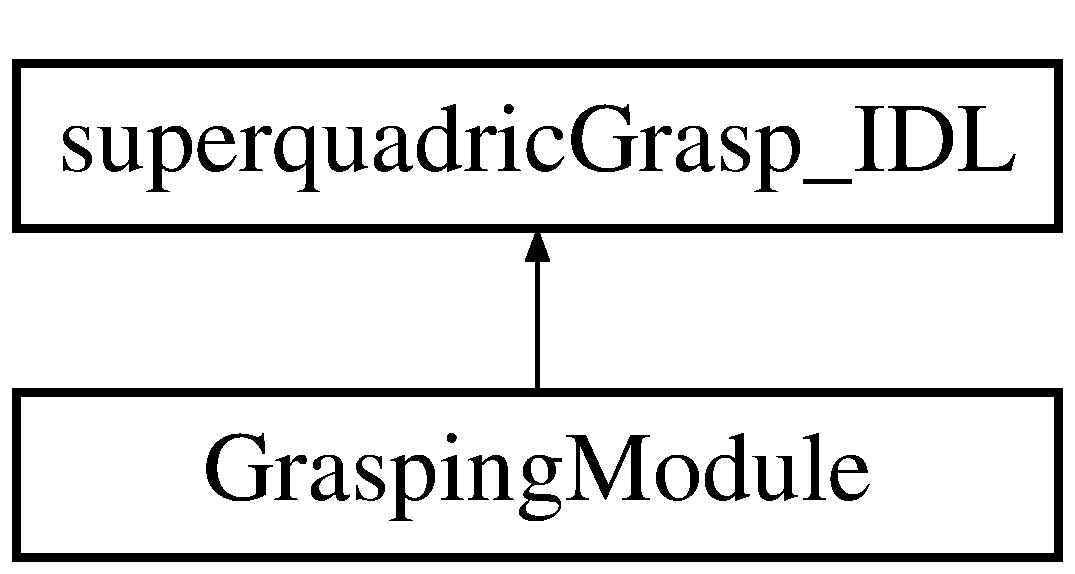
\includegraphics[height=2.000000cm]{classsuperquadricGrasp__IDL}
\end{center}
\end{figure}
\subsection*{Public Member Functions}
\begin{DoxyCompactItemize}
\item 
virtual bool \hyperlink{classsuperquadricGrasp__IDL_a6d1e4533ad8b34510ba9792f7cd72113}{clear\+\_\+poses} ()
\begin{DoxyCompactList}\small\item\em Remove computed poses. \end{DoxyCompactList}\item 
virtual bool \hyperlink{classsuperquadricGrasp__IDL_a6215b75f080a5837599b25826c142921}{set\+\_\+hand} (const std\+::string \&hand)
\begin{DoxyCompactList}\small\item\em Choose the hand to use to grasp the object. \end{DoxyCompactList}\item 
virtual std\+::string \hyperlink{classsuperquadricGrasp__IDL_ad1e5b402e403bc6765d7bf7e8fff0e91}{get\+\_\+hand} ()
\begin{DoxyCompactList}\small\item\em Get the chosen hand. \end{DoxyCompactList}\item 
virtual bool \hyperlink{classsuperquadricGrasp__IDL_ac01ec2012d2b12098a86f7f053068464}{set\+\_\+save\+\_\+poses} (const std\+::string \&entry)
\begin{DoxyCompactList}\small\item\em Set if to save or not the computed poses and trajectory. \end{DoxyCompactList}\item 
virtual std\+::string \hyperlink{classsuperquadricGrasp__IDL_aab45b0423b4e2d440b8a1256c1d6bdfc}{get\+\_\+save\+\_\+poses} ()
\begin{DoxyCompactList}\small\item\em Get if the saving process is on or off. \end{DoxyCompactList}\item 
virtual bool \hyperlink{classsuperquadricGrasp__IDL_a5320ef56cf3da687e7cf678b2a9397f5}{set\+\_\+options} (const yarp\+::os\+::\+Property \&options, const std\+::string \&field)
\begin{DoxyCompactList}\small\item\em Set the parameters of the module. \end{DoxyCompactList}\item 
virtual yarp\+::os\+::\+Property \hyperlink{classsuperquadricGrasp__IDL_a4799064cf16a52762787c0b245318d54}{get\+\_\+options} (const std\+::string \&field)
\begin{DoxyCompactList}\small\item\em Get the parameters of the module. \end{DoxyCompactList}\item 
virtual yarp\+::os\+::\+Property \hyperlink{classsuperquadricGrasp__IDL_a595e98ed2a8fca7ac707b71f97d626d1}{get\+\_\+grasping\+\_\+pose} (const yarp\+::os\+::\+Property \&estimated\+\_\+superq, const std\+::string \&hand)
\begin{DoxyCompactList}\small\item\em Return the estimated grasping poses given an estimated superquadric. \end{DoxyCompactList}\item 
virtual bool \hyperlink{classsuperquadricGrasp__IDL_a91d43de48ad97e35205010c7510e503c}{set\+\_\+visualization} (const std\+::string \&e)
\begin{DoxyCompactList}\small\item\em Set if the visualization has to be enabled. \end{DoxyCompactList}\item 
virtual std\+::string \hyperlink{classsuperquadricGrasp__IDL_ad108d67db8f389b630fa2b0caed87ca5}{get\+\_\+visualization} ()
\begin{DoxyCompactList}\small\item\em Get if visualization is enabled. \end{DoxyCompactList}\item 
virtual bool \hyperlink{classsuperquadricGrasp__IDL_aa996e476a845b484542c7a596cc1f02a}{move} (const std\+::string \&e)
\begin{DoxyCompactList}\small\item\em Move the right or the left arm (according to the string e). \end{DoxyCompactList}\item 
virtual bool {\bfseries look\+\_\+center} ()\label{classsuperquadricGrasp__IDL_a2f9efa6904f4e7240456a4968f3f6c07}

\item 
virtual bool {\bfseries look\+\_\+obj} ()\label{classsuperquadricGrasp__IDL_ad583966fde84372bad2b65214dcbe2bc}

\item 
virtual bool \hyperlink{classsuperquadricGrasp__IDL_a67b63b85635a02ab15f9447ad2b1b0dd}{go\+\_\+home} (const std\+::string \&e)
\begin{DoxyCompactList}\small\item\em Move the right or the left arm back to home position (according to the string e). \end{DoxyCompactList}\item 
virtual bool \hyperlink{classsuperquadricGrasp__IDL_abafbd89252eed10caf876ff1965491d0}{go\+\_\+to\+\_\+basket} (const std\+::string \&e)
\begin{DoxyCompactList}\small\item\em Move the right or the left arm to the basket (according to the string e). \end{DoxyCompactList}\item 
virtual std\+::string \hyperlink{classsuperquadricGrasp__IDL_afca9a01bade8e22262e5e70a96d671ae}{get\+\_\+best\+\_\+hand} ()
\begin{DoxyCompactList}\small\item\em Get the name of the best hand for grasping the object. \end{DoxyCompactList}\item 
virtual bool \hyperlink{classsuperquadricGrasp__IDL_afd0cc265ba84c844aee5654f1a713fbd}{check\+\_\+motion} ()
\begin{DoxyCompactList}\small\item\em Check if the motion has been completed. \end{DoxyCompactList}\item 
virtual bool \hyperlink{classsuperquadricGrasp__IDL_a9e11fd04a40c86987500c42f898508ea}{check\+\_\+home} ()
\begin{DoxyCompactList}\small\item\em Check if the motion back to home has been completed. \end{DoxyCompactList}\item 
virtual bool \hyperlink{classsuperquadricGrasp__IDL_ac40ef7c0dd4f0e3600db9aea5cc5c298}{calibrate} ()
\begin{DoxyCompactList}\small\item\em Calibrate plane height via superquadric computation. \end{DoxyCompactList}\item 
virtual bool {\bfseries read} (yarp\+::os\+::\+Connection\+Reader \&connection) Y\+A\+R\+P\+\_\+\+O\+V\+E\+R\+R\+I\+DE\label{classsuperquadricGrasp__IDL_a710271cfee0c9b1a31707d84f194b69b}

\item 
virtual std\+::vector$<$ std\+::string $>$ {\bfseries help} (const std\+::string \&function\+Name=\char`\"{}-\/-\/all\char`\"{})\label{classsuperquadricGrasp__IDL_a226f766d3a3a0ba87e7c1fa0aceb2cb8}

\end{DoxyCompactItemize}


\subsection{Detailed Description}
\hyperlink{classsuperquadricGrasp__IDL}{superquadric\+Grasp\+\_\+\+I\+DL} I\+DL Interface to superquadric-\/grasp services. 

Definition at line 18 of file superquadric\+Grasp\+\_\+\+I\+D\+L.\+h.



\subsection{Member Function Documentation}
\index{superquadric\+Grasp\+\_\+\+I\+DL@{superquadric\+Grasp\+\_\+\+I\+DL}!calibrate@{calibrate}}
\index{calibrate@{calibrate}!superquadric\+Grasp\+\_\+\+I\+DL@{superquadric\+Grasp\+\_\+\+I\+DL}}
\subsubsection[{\texorpdfstring{calibrate()}{calibrate()}}]{\setlength{\rightskip}{0pt plus 5cm}virtual bool superquadric\+Grasp\+\_\+\+I\+D\+L\+::calibrate (
\begin{DoxyParamCaption}
{}
\end{DoxyParamCaption}
)\hspace{0.3cm}{\ttfamily [virtual]}}\label{classsuperquadricGrasp__IDL_ac40ef7c0dd4f0e3600db9aea5cc5c298}


Calibrate plane height via superquadric computation. 

\begin{DoxyReturn}{Returns}
true/false on success/failure. 
\end{DoxyReturn}
\index{superquadric\+Grasp\+\_\+\+I\+DL@{superquadric\+Grasp\+\_\+\+I\+DL}!check\+\_\+home@{check\+\_\+home}}
\index{check\+\_\+home@{check\+\_\+home}!superquadric\+Grasp\+\_\+\+I\+DL@{superquadric\+Grasp\+\_\+\+I\+DL}}
\subsubsection[{\texorpdfstring{check\+\_\+home()}{check_home()}}]{\setlength{\rightskip}{0pt plus 5cm}virtual bool superquadric\+Grasp\+\_\+\+I\+D\+L\+::check\+\_\+home (
\begin{DoxyParamCaption}
{}
\end{DoxyParamCaption}
)\hspace{0.3cm}{\ttfamily [virtual]}}\label{classsuperquadricGrasp__IDL_a9e11fd04a40c86987500c42f898508ea}


Check if the motion back to home has been completed. 

\begin{DoxyReturn}{Returns}
true/false on success/failure 
\end{DoxyReturn}


Reimplemented in \hyperlink{classGraspingModule_a650c026153e3a7b0044f508cf9d4bf00}{Grasping\+Module}.

\index{superquadric\+Grasp\+\_\+\+I\+DL@{superquadric\+Grasp\+\_\+\+I\+DL}!check\+\_\+motion@{check\+\_\+motion}}
\index{check\+\_\+motion@{check\+\_\+motion}!superquadric\+Grasp\+\_\+\+I\+DL@{superquadric\+Grasp\+\_\+\+I\+DL}}
\subsubsection[{\texorpdfstring{check\+\_\+motion()}{check_motion()}}]{\setlength{\rightskip}{0pt plus 5cm}virtual bool superquadric\+Grasp\+\_\+\+I\+D\+L\+::check\+\_\+motion (
\begin{DoxyParamCaption}
{}
\end{DoxyParamCaption}
)\hspace{0.3cm}{\ttfamily [virtual]}}\label{classsuperquadricGrasp__IDL_afd0cc265ba84c844aee5654f1a713fbd}


Check if the motion has been completed. 

\begin{DoxyReturn}{Returns}
true/false on success/failure 
\end{DoxyReturn}


Reimplemented in \hyperlink{classGraspingModule_a91eac72e632f224442f34b907e479fa3}{Grasping\+Module}.

\index{superquadric\+Grasp\+\_\+\+I\+DL@{superquadric\+Grasp\+\_\+\+I\+DL}!clear\+\_\+poses@{clear\+\_\+poses}}
\index{clear\+\_\+poses@{clear\+\_\+poses}!superquadric\+Grasp\+\_\+\+I\+DL@{superquadric\+Grasp\+\_\+\+I\+DL}}
\subsubsection[{\texorpdfstring{clear\+\_\+poses()}{clear_poses()}}]{\setlength{\rightskip}{0pt plus 5cm}virtual bool superquadric\+Grasp\+\_\+\+I\+D\+L\+::clear\+\_\+poses (
\begin{DoxyParamCaption}
{}
\end{DoxyParamCaption}
)\hspace{0.3cm}{\ttfamily [virtual]}}\label{classsuperquadricGrasp__IDL_a6d1e4533ad8b34510ba9792f7cd72113}


Remove computed poses. 

\begin{DoxyReturn}{Returns}
true/false on success/failure. 
\end{DoxyReturn}


Reimplemented in \hyperlink{classGraspingModule_a834e972a2a1b7b92bf8dc1e83319b028}{Grasping\+Module}.

\index{superquadric\+Grasp\+\_\+\+I\+DL@{superquadric\+Grasp\+\_\+\+I\+DL}!get\+\_\+best\+\_\+hand@{get\+\_\+best\+\_\+hand}}
\index{get\+\_\+best\+\_\+hand@{get\+\_\+best\+\_\+hand}!superquadric\+Grasp\+\_\+\+I\+DL@{superquadric\+Grasp\+\_\+\+I\+DL}}
\subsubsection[{\texorpdfstring{get\+\_\+best\+\_\+hand()}{get_best_hand()}}]{\setlength{\rightskip}{0pt plus 5cm}virtual std\+::string superquadric\+Grasp\+\_\+\+I\+D\+L\+::get\+\_\+best\+\_\+hand (
\begin{DoxyParamCaption}
{}
\end{DoxyParamCaption}
)\hspace{0.3cm}{\ttfamily [virtual]}}\label{classsuperquadricGrasp__IDL_afca9a01bade8e22262e5e70a96d671ae}


Get the name of the best hand for grasping the object. 

\begin{DoxyReturn}{Returns}
right or left 
\end{DoxyReturn}


Reimplemented in \hyperlink{classGraspingModule_a5103f8bd6671a11a9bd1c7e29d290009}{Grasping\+Module}.

\index{superquadric\+Grasp\+\_\+\+I\+DL@{superquadric\+Grasp\+\_\+\+I\+DL}!get\+\_\+grasping\+\_\+pose@{get\+\_\+grasping\+\_\+pose}}
\index{get\+\_\+grasping\+\_\+pose@{get\+\_\+grasping\+\_\+pose}!superquadric\+Grasp\+\_\+\+I\+DL@{superquadric\+Grasp\+\_\+\+I\+DL}}
\subsubsection[{\texorpdfstring{get\+\_\+grasping\+\_\+pose(const yarp\+::os\+::\+Property \&estimated\+\_\+superq, const std\+::string \&hand)}{get_grasping_pose(const yarp::os::Property &estimated_superq, const std::string &hand)}}]{\setlength{\rightskip}{0pt plus 5cm}virtual yarp\+::os\+::\+Property superquadric\+Grasp\+\_\+\+I\+D\+L\+::get\+\_\+grasping\+\_\+pose (
\begin{DoxyParamCaption}
\item[{const yarp\+::os\+::\+Property \&}]{estimated\+\_\+superq, }
\item[{const std\+::string \&}]{hand}
\end{DoxyParamCaption}
)\hspace{0.3cm}{\ttfamily [virtual]}}\label{classsuperquadricGrasp__IDL_a595e98ed2a8fca7ac707b71f97d626d1}


Return the estimated grasping poses given an estimated superquadric. 


\begin{DoxyParams}{Parameters}
{\em estimated\+\_\+superq} & is a Property containing the superquadric. \\
\hline
{\em hand} & is the hand for which we want to solve the grasping problem (right, left or both). \\
\hline
\end{DoxyParams}
\begin{DoxyReturn}{Returns}
a property containing the solution. Note\+: the estimated superquadric must be provide in the following format\+: (dimensions (x0 x1 x2)) (exponents (x3 x4)) (center (x5 x6 x7)) (orientation (x8 x9 x10 x11)) where x0, x1,x2 are the semi axes of the superquadric, x3, x4 are the responsible for the shape, x5 x6 x7 are the coordinates of the superquadric center and x8 x9 x10 x11 are the axis-\/angle representation of the superquadric orientation. The solution is given in the form\+: (pose\+\_\+right (h0 h1 h2 h3 h4 h5 h6)) (trajectory\+\_\+right (t0 t1 t2 t3 t4 t5) ... ) for the right hand, and the same for the left hand (according to the value of the string hand are input parameter. The quantity \char`\"{}pose\+\_\+right\char`\"{} is the pose computed for the robot hand (x0,x1,x2, are the 3D coordinates of the end-\/effector and x3,x4,x5 are the Euler angles representing the end-\/effector orientation) The quantity \char`\"{}trajectory\+\_\+right\char`\"{} includes all the waypoint of the computed trajectory, in the form center of the end-\/effector (t0,t1,t2)+ orientation (Euler angles, t3,t4,t5). 
\end{DoxyReturn}


Reimplemented in \hyperlink{classGraspingModule_af1e057f767ab83be185cf486d3f5c46b}{Grasping\+Module}.

\index{superquadric\+Grasp\+\_\+\+I\+DL@{superquadric\+Grasp\+\_\+\+I\+DL}!get\+\_\+hand@{get\+\_\+hand}}
\index{get\+\_\+hand@{get\+\_\+hand}!superquadric\+Grasp\+\_\+\+I\+DL@{superquadric\+Grasp\+\_\+\+I\+DL}}
\subsubsection[{\texorpdfstring{get\+\_\+hand()}{get_hand()}}]{\setlength{\rightskip}{0pt plus 5cm}virtual std\+::string superquadric\+Grasp\+\_\+\+I\+D\+L\+::get\+\_\+hand (
\begin{DoxyParamCaption}
{}
\end{DoxyParamCaption}
)\hspace{0.3cm}{\ttfamily [virtual]}}\label{classsuperquadricGrasp__IDL_ad1e5b402e403bc6765d7bf7e8fff0e91}


Get the chosen hand. 

\begin{DoxyReturn}{Returns}
left or right. 
\end{DoxyReturn}


Reimplemented in \hyperlink{classGraspingModule_a557a87131c7396dd62c02eced7f4a937}{Grasping\+Module}.

\index{superquadric\+Grasp\+\_\+\+I\+DL@{superquadric\+Grasp\+\_\+\+I\+DL}!get\+\_\+options@{get\+\_\+options}}
\index{get\+\_\+options@{get\+\_\+options}!superquadric\+Grasp\+\_\+\+I\+DL@{superquadric\+Grasp\+\_\+\+I\+DL}}
\subsubsection[{\texorpdfstring{get\+\_\+options(const std\+::string \&field)}{get_options(const std::string &field)}}]{\setlength{\rightskip}{0pt plus 5cm}virtual yarp\+::os\+::\+Property superquadric\+Grasp\+\_\+\+I\+D\+L\+::get\+\_\+options (
\begin{DoxyParamCaption}
\item[{const std\+::string \&}]{field}
\end{DoxyParamCaption}
)\hspace{0.3cm}{\ttfamily [virtual]}}\label{classsuperquadricGrasp__IDL_a4799064cf16a52762787c0b245318d54}


Get the parameters of the module. 

The user must pay attention in changing them. 
\begin{DoxyParams}{Parameters}
{\em field} & can be \char`\"{}pose\char`\"{}, \char`\"{}trajectory\char`\"{}, \char`\"{}optimization\char`\"{}, \char`\"{}statistics\char`\"{}, \char`\"{}visualization\char`\"{} or \char`\"{}execution\char`\"{}. depending on which parameters we are interested in. \\
\hline
\end{DoxyParams}
\begin{DoxyReturn}{Returns}
the Property including all the parameter values. 
\end{DoxyReturn}


Reimplemented in \hyperlink{classGraspingModule_a375475691c644d8aa882db8d65ceda50}{Grasping\+Module}.

\index{superquadric\+Grasp\+\_\+\+I\+DL@{superquadric\+Grasp\+\_\+\+I\+DL}!get\+\_\+save\+\_\+poses@{get\+\_\+save\+\_\+poses}}
\index{get\+\_\+save\+\_\+poses@{get\+\_\+save\+\_\+poses}!superquadric\+Grasp\+\_\+\+I\+DL@{superquadric\+Grasp\+\_\+\+I\+DL}}
\subsubsection[{\texorpdfstring{get\+\_\+save\+\_\+poses()}{get_save_poses()}}]{\setlength{\rightskip}{0pt plus 5cm}virtual std\+::string superquadric\+Grasp\+\_\+\+I\+D\+L\+::get\+\_\+save\+\_\+poses (
\begin{DoxyParamCaption}
{}
\end{DoxyParamCaption}
)\hspace{0.3cm}{\ttfamily [virtual]}}\label{classsuperquadricGrasp__IDL_aab45b0423b4e2d440b8a1256c1d6bdfc}


Get if the saving process is on or off. 

\begin{DoxyReturn}{Returns}
\char`\"{}on\char`\"{} or \char`\"{}off\char`\"{}. 
\end{DoxyReturn}


Reimplemented in \hyperlink{classGraspingModule_a949e4297bdf26f564669ffc91068c4f3}{Grasping\+Module}.

\index{superquadric\+Grasp\+\_\+\+I\+DL@{superquadric\+Grasp\+\_\+\+I\+DL}!get\+\_\+visualization@{get\+\_\+visualization}}
\index{get\+\_\+visualization@{get\+\_\+visualization}!superquadric\+Grasp\+\_\+\+I\+DL@{superquadric\+Grasp\+\_\+\+I\+DL}}
\subsubsection[{\texorpdfstring{get\+\_\+visualization()}{get_visualization()}}]{\setlength{\rightskip}{0pt plus 5cm}virtual std\+::string superquadric\+Grasp\+\_\+\+I\+D\+L\+::get\+\_\+visualization (
\begin{DoxyParamCaption}
{}
\end{DoxyParamCaption}
)\hspace{0.3cm}{\ttfamily [virtual]}}\label{classsuperquadricGrasp__IDL_ad108d67db8f389b630fa2b0caed87ca5}


Get if visualization is enabled. 

\begin{DoxyReturn}{Returns}
\char`\"{}on\char`\"{} or \char`\"{}off\char`\"{}. 
\end{DoxyReturn}


Reimplemented in \hyperlink{classGraspingModule_aabedec650875263d27ecf20fa9dd8b39}{Grasping\+Module}.

\index{superquadric\+Grasp\+\_\+\+I\+DL@{superquadric\+Grasp\+\_\+\+I\+DL}!go\+\_\+home@{go\+\_\+home}}
\index{go\+\_\+home@{go\+\_\+home}!superquadric\+Grasp\+\_\+\+I\+DL@{superquadric\+Grasp\+\_\+\+I\+DL}}
\subsubsection[{\texorpdfstring{go\+\_\+home(const std\+::string \&e)}{go_home(const std::string &e)}}]{\setlength{\rightskip}{0pt plus 5cm}virtual bool superquadric\+Grasp\+\_\+\+I\+D\+L\+::go\+\_\+home (
\begin{DoxyParamCaption}
\item[{const std\+::string \&}]{e}
\end{DoxyParamCaption}
)\hspace{0.3cm}{\ttfamily [virtual]}}\label{classsuperquadricGrasp__IDL_a67b63b85635a02ab15f9447ad2b1b0dd}


Move the right or the left arm back to home position (according to the string e). 

\begin{DoxyReturn}{Returns}
\char`\"{}on\char`\"{} or \char`\"{}off\char`\"{} if e is right or left. 
\end{DoxyReturn}


Reimplemented in \hyperlink{classGraspingModule_a1455fc4c6a1ae5690fa691cc324fec4e}{Grasping\+Module}.

\index{superquadric\+Grasp\+\_\+\+I\+DL@{superquadric\+Grasp\+\_\+\+I\+DL}!go\+\_\+to\+\_\+basket@{go\+\_\+to\+\_\+basket}}
\index{go\+\_\+to\+\_\+basket@{go\+\_\+to\+\_\+basket}!superquadric\+Grasp\+\_\+\+I\+DL@{superquadric\+Grasp\+\_\+\+I\+DL}}
\subsubsection[{\texorpdfstring{go\+\_\+to\+\_\+basket(const std\+::string \&e)}{go_to_basket(const std::string &e)}}]{\setlength{\rightskip}{0pt plus 5cm}virtual bool superquadric\+Grasp\+\_\+\+I\+D\+L\+::go\+\_\+to\+\_\+basket (
\begin{DoxyParamCaption}
\item[{const std\+::string \&}]{e}
\end{DoxyParamCaption}
)\hspace{0.3cm}{\ttfamily [virtual]}}\label{classsuperquadricGrasp__IDL_abafbd89252eed10caf876ff1965491d0}


Move the right or the left arm to the basket (according to the string e). 

\begin{DoxyReturn}{Returns}
\char`\"{}on\char`\"{} or \char`\"{}off\char`\"{} if e is right or left. 
\end{DoxyReturn}


Reimplemented in \hyperlink{classGraspingModule_a75482819f7f289b3f456571628952122}{Grasping\+Module}.

\index{superquadric\+Grasp\+\_\+\+I\+DL@{superquadric\+Grasp\+\_\+\+I\+DL}!move@{move}}
\index{move@{move}!superquadric\+Grasp\+\_\+\+I\+DL@{superquadric\+Grasp\+\_\+\+I\+DL}}
\subsubsection[{\texorpdfstring{move(const std\+::string \&e)}{move(const std::string &e)}}]{\setlength{\rightskip}{0pt plus 5cm}virtual bool superquadric\+Grasp\+\_\+\+I\+D\+L\+::move (
\begin{DoxyParamCaption}
\item[{const std\+::string \&}]{e}
\end{DoxyParamCaption}
)\hspace{0.3cm}{\ttfamily [virtual]}}\label{classsuperquadricGrasp__IDL_aa996e476a845b484542c7a596cc1f02a}


Move the right or the left arm (according to the string e). 

\begin{DoxyReturn}{Returns}
\char`\"{}on\char`\"{} or \char`\"{}off\char`\"{} if e is right or left. 
\end{DoxyReturn}


Reimplemented in \hyperlink{classGraspingModule_a08bd9cdbb1d16da8616c9769510e2bf1}{Grasping\+Module}.

\index{superquadric\+Grasp\+\_\+\+I\+DL@{superquadric\+Grasp\+\_\+\+I\+DL}!set\+\_\+hand@{set\+\_\+hand}}
\index{set\+\_\+hand@{set\+\_\+hand}!superquadric\+Grasp\+\_\+\+I\+DL@{superquadric\+Grasp\+\_\+\+I\+DL}}
\subsubsection[{\texorpdfstring{set\+\_\+hand(const std\+::string \&hand)}{set_hand(const std::string &hand)}}]{\setlength{\rightskip}{0pt plus 5cm}virtual bool superquadric\+Grasp\+\_\+\+I\+D\+L\+::set\+\_\+hand (
\begin{DoxyParamCaption}
\item[{const std\+::string \&}]{hand}
\end{DoxyParamCaption}
)\hspace{0.3cm}{\ttfamily [virtual]}}\label{classsuperquadricGrasp__IDL_a6215b75f080a5837599b25826c142921}


Choose the hand to use to grasp the object. 


\begin{DoxyParams}{Parameters}
{\em hand} & name (left or right). \\
\hline
\end{DoxyParams}
\begin{DoxyReturn}{Returns}
true/false on success/failure. 
\end{DoxyReturn}


Reimplemented in \hyperlink{classGraspingModule_a9d34cb0521f86dd16648255e640eec90}{Grasping\+Module}.

\index{superquadric\+Grasp\+\_\+\+I\+DL@{superquadric\+Grasp\+\_\+\+I\+DL}!set\+\_\+options@{set\+\_\+options}}
\index{set\+\_\+options@{set\+\_\+options}!superquadric\+Grasp\+\_\+\+I\+DL@{superquadric\+Grasp\+\_\+\+I\+DL}}
\subsubsection[{\texorpdfstring{set\+\_\+options(const yarp\+::os\+::\+Property \&options, const std\+::string \&field)}{set_options(const yarp::os::Property &options, const std::string &field)}}]{\setlength{\rightskip}{0pt plus 5cm}virtual bool superquadric\+Grasp\+\_\+\+I\+D\+L\+::set\+\_\+options (
\begin{DoxyParamCaption}
\item[{const yarp\+::os\+::\+Property \&}]{options, }
\item[{const std\+::string \&}]{field}
\end{DoxyParamCaption}
)\hspace{0.3cm}{\ttfamily [virtual]}}\label{classsuperquadricGrasp__IDL_a5320ef56cf3da687e7cf678b2a9397f5}


Set the parameters of the module. 

The user must pay attention in changing them. 
\begin{DoxyParams}{Parameters}
{\em options} & is a Property containing the parameters the user want to change. \\
\hline
{\em field} & is a string specifying which can of parameter we are going to change. Field can be\+: \char`\"{}pose\char`\"{}, \char`\"{}trajectory\char`\"{}, \char`\"{}optimization\char`\"{}, \char`\"{}visualization\char`\"{} or \char`\"{}execution\char`\"{}. You can set the parameters typing, for instance\+: command\+: set\+\_\+options ((n\+\_\+pointshand $<$points-\/value$>$) (hand\+\_\+displacement\+\_\+x $<$displacement-\/value$>$)) pose. \\
\hline
\end{DoxyParams}
\begin{DoxyReturn}{Returns}
true/false on success/failure. 
\end{DoxyReturn}


Reimplemented in \hyperlink{classGraspingModule_a849c459ef9700c93b45ef6cff394f675}{Grasping\+Module}.

\index{superquadric\+Grasp\+\_\+\+I\+DL@{superquadric\+Grasp\+\_\+\+I\+DL}!set\+\_\+save\+\_\+poses@{set\+\_\+save\+\_\+poses}}
\index{set\+\_\+save\+\_\+poses@{set\+\_\+save\+\_\+poses}!superquadric\+Grasp\+\_\+\+I\+DL@{superquadric\+Grasp\+\_\+\+I\+DL}}
\subsubsection[{\texorpdfstring{set\+\_\+save\+\_\+poses(const std\+::string \&entry)}{set_save_poses(const std::string &entry)}}]{\setlength{\rightskip}{0pt plus 5cm}virtual bool superquadric\+Grasp\+\_\+\+I\+D\+L\+::set\+\_\+save\+\_\+poses (
\begin{DoxyParamCaption}
\item[{const std\+::string \&}]{entry}
\end{DoxyParamCaption}
)\hspace{0.3cm}{\ttfamily [virtual]}}\label{classsuperquadricGrasp__IDL_ac01ec2012d2b12098a86f7f053068464}


Set if to save or not the computed poses and trajectory. 


\begin{DoxyParams}{Parameters}
{\em entry} & can be \char`\"{}on\char`\"{} or \char`\"{}off\char`\"{}. \\
\hline
\end{DoxyParams}
\begin{DoxyReturn}{Returns}
true/false on success/failure. 
\end{DoxyReturn}


Reimplemented in \hyperlink{classGraspingModule_a618785dec349358760a05e6e4b097866}{Grasping\+Module}.

\index{superquadric\+Grasp\+\_\+\+I\+DL@{superquadric\+Grasp\+\_\+\+I\+DL}!set\+\_\+visualization@{set\+\_\+visualization}}
\index{set\+\_\+visualization@{set\+\_\+visualization}!superquadric\+Grasp\+\_\+\+I\+DL@{superquadric\+Grasp\+\_\+\+I\+DL}}
\subsubsection[{\texorpdfstring{set\+\_\+visualization(const std\+::string \&e)}{set_visualization(const std::string &e)}}]{\setlength{\rightskip}{0pt plus 5cm}virtual bool superquadric\+Grasp\+\_\+\+I\+D\+L\+::set\+\_\+visualization (
\begin{DoxyParamCaption}
\item[{const std\+::string \&}]{e}
\end{DoxyParamCaption}
)\hspace{0.3cm}{\ttfamily [virtual]}}\label{classsuperquadricGrasp__IDL_a91d43de48ad97e35205010c7510e503c}


Set if the visualization has to be enabled. 

\begin{DoxyReturn}{Returns}
true/false on success/failure. 
\end{DoxyReturn}


Reimplemented in \hyperlink{classGraspingModule_a801de4b63aba360a4b85e322c5947a4a}{Grasping\+Module}.



The documentation for this class was generated from the following file\+:\begin{DoxyCompactItemize}
\item 
/home/gvezzani/\+Desktop/\+Ph\+D/\+Anno\+\_\+1/super\+Quadratiche/superquadric-\/grasp/idl\+\_\+dox/superquadric\+Grasp\+\_\+\+I\+D\+L.\+h\end{DoxyCompactItemize}

%--- End generated contents ---

% Index
\backmatter
\newpage
\phantomsection
\clearemptydoublepage
\addcontentsline{toc}{chapter}{Index}
\printindex

\end{document}
